% =============================================================================
% GEODERMA MANUSCRIPT TEMPLATE
% Elsevier elsarticle class
% =============================================================================

\documentclass[preprint,12pt]{elsarticle}

% -----------------------------------------------------------------------------
% 1. PACKAGES
% -----------------------------------------------------------------------------

% Mathematics
\usepackage{amsmath}
\usepackage{amssymb}
\usepackage{mathtools}

% Figures
\usepackage{graphicx}
\usepackage{float}
\usepackage{subcaption}

% Tables
\usepackage{booktabs}
\usepackage{tabularx}
\usepackage{array}
\usepackage{multirow}
\usepackage{threeparttable}
\usepackage{makecell}
\usepackage{pdflscape}
\usepackage{array}
\usepackage{longtable}

% SI units
\usepackage{siunitx}
\sisetup{
    detect-all,
    separate-uncertainty = true
}

% Text formatting
\usepackage{lineno}
\usepackage{microtype}

% Hyperlinks and cross-referencing
\usepackage[colorlinks=true,
            linkcolor=blue,
            citecolor=blue,
            urlcolor=blue]{hyperref}

\usepackage[nameinlink,noabbrev]{cleveref}

% Supplementary
\usepackage{hyperref}
\usepackage{xr}
\usepackage[nameinlink,noabbrev]{cleveref}
% -----------------------------------------------------------------------------
% 2. JOURNAL AND BIBLIOGRAPHY SETTINGS
% -----------------------------------------------------------------------------

% Elsevier bibliography style
% Use numerical citations: [1], [2], [3]
\bibliographystyle{elsarticle-num}

% -----------------------------------------------------------------------------
% 3. JOURNAL METADATA
% -----------------------------------------------------------------------------

\journal{Geoderma}

% -----------------------------------------------------------------------------
% TITLE AND AUTHORS
% -----------------------------------------------------------------------------
\begin{document}
\begin{frontmatter}

\title{Mineralogy-dependent effects of silicate amendments on soil organic carbon allocation and persistence}

\author[aff1]{Teneille Nel\corref{cor1}}
\ead{first.author@email.com}

\author[aff1]{Lucilla Boito}
\ead{second.author@email.com}

\author[aff1]{Laura Steinwidder}

\author[aff2]{Carlos A. Sierra}

\author[aff1]{Sara Vicca}

\address[aff1]{
    Department of Soil Science,
    University Name,
    City,
    Country
}

\address[aff2]{
    Department of Environmental Science,
    University Name,
    City,
    Country
}

\cortext[cor1]{Corresponding author}

\begin{abstract}

Enhanced rock weathering (ERW) using crushed silicate rocks is increasingly investigated as a strategy for atmospheric $\text{CO}_2$ removal, but its effects on existing soil organic carbon (SOC) dynamics remain poorly understood. We examined how three silicate amendments with contrasting mineralogies –nepheline-rich Bolsdorfer basalt, 2:1-phyllosilicate- and forsterite-bearing H\"uhnerberg basalt, and plagioclase- and leucite-bearing Eifelgold tephrite – alongside agricultural lime, influenced soil geochemistry, SOC fractions and carbon turnover three years after application in a field experiment. Soil geochemical analyses, density fractionation, attenuated total reflectance Fourier-transform infrared (ATR-FTIR) spectroscopy and radiocarbon ($\Delta^{14}\text{C}$) measurements were combined with compartmental carbon turnover modelling (SoilR). Feedstock mineralogy governed distinct geochemical responses: Bolsdorfer increased pH, exchangeable Na$^{+}$/K$^{+}$, and oxalate-extractable Si; H\"uhnerberg enriched exchangeable Mg$^{2+}$ and reduced porewater Al; and Eifelgold produced more modest shifts in extractable and exchangeable cations, consistent with its lower proportion of rapidly weathering feldspathoids. While bulk SOC, occluded particulate organic matter (oPOM)-C and mineral-associated organic matter (MAOM)-C showed no clear treatment-related differences, free particulate organic matter (fPOM)-C increased under H\"uhnerberg and Bolsdorfer. Modelled carbon dynamics further revealed contrasting responses among amendments. Eifelgold and lime yielded the longest estimated system carbon transit times and higher carbon transfer from oPOM to MAOM. H\"uhnerberg increased fPOM-C and aggregate stability tendencies, but was associated with a higher modelled MAOM decomposition rate, consistent with weaker outer-sphere or Mg-bridged sorption onto exogenous 2:1 phyllosilicates. Conversely, Bolsdorfer showed little change in oPOM-to-MAOM transfer despite feldspathoid weathering, potentially reflecting monovalent Na$^{+}$-induced dispersion. Across treatments, modelled fPOM decomposition rates were higher and oPOM decomposition rates tended to be lower than in the control, while carbon transfer and turnover covaried with extractable cations, secondary mineral indicators and FTIR-derived carboxylate, carbonyl and polysaccharide shifts. Overall, silicate amendments influence soil carbon cycling through mineralogy-dependent weathering pathways and organo-mineral bonding environments, demonstrating that feedstock selection must account for both inorganic carbon removal and SOC persistence.

\end{abstract}


\begin{keyword}
Soil organic carbon
\sep Enhanced rock weathering
\sep Soil geochemistry
\sep Carbon persistence
\end{keyword}

\end{frontmatter}
% -----------------------------------------------------------------------------
% 7. MAIN TEXT
% -----------------------------------------------------------------------------

% Uncomment for line numbering during manuscript review
% \linenumbers

\section{Introduction}
\label{sec:introduction}

Significant increases in atmospheric CO$_2$ concentrations since the Industrial Revolution necessitate effective carbon dioxide removal (CDR) technologies. Enhanced rock weathering (ERW), which involves the application of crushed silicate rocks to soils, has the potential to contribute to long-term atmospheric CO$_2$ removal by accelerating natural silicate weathering \citep{Hartmann2008,manning2024soil}. During this process, atmospheric CO$_2$ is converted into dissolved bicarbonate, which can subsequently contribute to inorganic carbon storage through carbonate formation, as illustrated by the following reaction:

\begin{equation}
    \mathrm{CaSiO_3 + CO_2 + 2H_2O
    \rightarrow CaCO_3 + H_4SiO_4}
    \label{eq:carbonation}
\end{equation}

Agricultural soils are particularly suitable for ERW and soil carbon sequestration (SCS) due to the extensive land area available and the potential synergies with existing agricultural management practices. Although ERW research has traditionally focused on inorganic carbon (C) sequestration, recent studies have demonstrated that silicate rock amendments can also substantially influence soil organic matter (SOM) dynamics, potentially affecting organic C fluxes several orders of magnitude greater than those associated with soil inorganic carbon (SIC) fluxes. These effects may result in either increases or losses of SOM stocks \citep{Vicca2022, steinwidder2025beyond,sokol2024reduced}. Understanding the effects of ERW on SOM dynamics is therefore essential for accurate net C accounting \citep{Niron2024}, particularly because increases in soil organic carbon (SOC) stocks may generate additional carbon credits independently of those associated with ERW-driven SIC sequestration \citep{manning2024soil}.

The effects of ERW on SOM are governed by competing mechanisms that may either promote SOC stabilization or accelerate its mineralization. The release of divalent cations during silicate weathering can enhance organo-mineral associations through electrostatic cation bridging between organic matter and clay mineral surfaces. Furthermore, the formation of secondary minerals, including Al/Fe (oxy)(hydr)oxides, may provide additional sorption surfaces for SOM stabilization as mineral-associated organic matter (MAOM) \citep{Vienne2025}. Conversely, increases in soil pH and the release of micronutrients may stimulate microbial activity and SOM decomposition. Enhanced production of organic acids by plant roots and microorganisms during nutrient acquisition from rock amendments may also destabilize existing mineral-organic associations, promoting the desorption of previously protected organic C and exposing it to microbial decomposition \citep{Niron2024,sokol2024reduced}. Additionally, increases in plant productivity and organic matter inputs may stimulate decomposition losses through enhanced microbial activity \citep{stoner2021turnover}. Consequently, the net effect of ERW on SOC stocks depends not only on the magnitude of C inputs and losses but also on the mechanisms governing SOM formation and persistence.

\subsection{SOM persistence and carbon stability pools}

The persistence of SOC is fundamentally governed by its susceptibility to microbial decomposition and the environmental and physicochemical conditions that regulate its accessibility and stabilization. Six broad categories of controls on SOM persistence were recently summarized by \citep{rocci2024bridging}: physical inaccessibility, organo-mineral and -metal stabilization, biodegradability of plant inputs, abiotic environmental factors (climate and soil chemistry), biochemical reactivity and diversity (recalcitrance), and microbial physiology and morphology. Given the substantial heterogeneity of SOM, separating it into distinct components that differ in their formation, function, and persistence is necessary to accurately predict the vulnerability of bulk SOC to environmental change \citep{lavallee2019conceptualizing}.

In particular, particulate organic matter (POM) and MAOM represent functionally distinct SOC pools with different stabilization mechanisms. POM persistence is primarily associated with the biochemical characteristics of organic matter and its physical protection within soil aggregates, whereas MAOM generally comprises relatively simple molecular compounds stabilized through interactions with mineral surfaces. These interactions include van der Waals forces, hydrogen bonding, covalent bonding, complexation, cation bridging, and pore sorption. Distinguishing between these SOC fractions is therefore essential for identifying how ERW influences the formation and persistence of different organic C pools and for evaluating the mechanisms responsible for changes in bulk SOC stability.

\subsection{Assessing SOC persistence using radiocarbon}

Quantifying both net C inputs and the transit time of C in soils is essential for evaluating the effectiveness of soil C sequestration strategies in mitigating climate change \citep{sierra2021climate,xia2013traceable}. Although the effects of ERW on SOC accrual are increasingly being investigated \citep{Boito2025,steinwidder2025beyond}, the persistence of ERW-associated SOC remains poorly constrained. Assigning a precise stabilization time to SOC is particularly challenging and requires further research \citep{manning2024soil}. This uncertainty is especially relevant for topsoil SOM, which is in direct contact with the atmosphere and is consequently particularly vulnerable to decomposition \citep{mills2014longterm}.

While fast-cycling SOC pools can be investigated through relatively short-term experiments, the majority of soil C is stored in slower-cycling pools that are less amenable to experimental investigation \citep{mills2014longterm}. Radiocarbon ($^{14}$C) measurements, combined with observed SOC stocks, provide a means of constraining models of SOM dynamics over longer timescales, assuming steady-state conditions \citep{sierra2014radiocarbon}. Naturally occurring $^{14}$C decay can be used to estimate centennial-scale turnover, whereas the anthropogenic bomb-$^{14}$C spike associated with atmospheric nuclear testing during the mid-twentieth century provides information on SOC dynamics over decadal timescales \citep{mills2014longterm}. Integrating radiocarbon measurements with SOC fractionation and modelling approaches can therefore provide insights into the persistence of distinct SOC pools and their responses to ERW-induced changes in soil properties.

\subsection{Soil pH as a driver of SOC stabilization and destabilization}

Soil pH is a major determinant of the mechanisms governing SOC stabilization and decomposition. As pH increases, the dominant mechanisms of SOC stabilization may shift from organo-metal complexation, primarily involving carboxyl coordination and hydrogen bonding, towards associations with short-range-order (SRO) mineral phases and, subsequently, Ca complexation and cation bridging with phyllosilicates \citep{zhou2024global,Rasmussen2018,jiang2026molecular}. Increasing pH promotes the deprotonation of carboxyl groups, potentially enhancing electrostatic repulsion and destabilizing mineral-organic associations, thereby decreasing MAOM accumulation \citep{jiang2026molecular}. In addition, soil pH regulates microbial diversity and activity and is consequently an important driver of SOM decomposition \citep{Wang2024}.

Evidence from ERW experiments suggests that pH-induced changes in mineral-organic interactions may result in SOC destabilization. For example, \citep{steinwidder2025beyond} reported evidence of SOC release from MAOM following an increase in soil pH associated with silicate rock powder amendments. However, the consequences of increased rhizosphere respiration for SOC stocks are not necessarily negative, as enhanced respiration is often accompanied by increased photosynthesis and C inputs, potentially offsetting decomposition losses \citep{Kuzyakov2001}. Moreover, roots and rhizodeposits represent important precursors of MAOM and contribute to aggregate formation \citep{Leuthold2026, Sokol2022}. Organic matter may also facilitate mineral nucleation and transformation, further influencing the formation and persistence of organo-mineral associations \citep{kleber2021dynamic}. Thus, the net effect of ERW-induced pH changes on SOC persistence likely depends on the balance between destabilization of existing associations, enhanced microbial decomposition, and the formation of new mineral-organic associations.

\subsection{Secondary mineral formation and SOC stabilization}

ERW can accelerate mineral dissolution beyond natural weathering rates, increasing soil solution solute concentrations and potentially reducing primary mineral dissolution rates while stimulating the formation of secondary minerals \citep{Andrews2019,steinwidder2025beyond}. The subglacial grinding of bedrock has been shown to produce amorphous Si, Al, and Fe phases that may act as precursors to more crystalline phases, including phyllosilicates \citep{Behrens2015}. The formation of secondary clay minerals during ERW may subsequently influence weathering rates and reduce the efficacy of inorganic CDR \citep{manning2024soil}. However, the formation of reactive SRO metal oxides, such as allophane and ferrihydrite, and aluminosilicates, such as proto-imogolite, may provide additional mineral surfaces for SOM sorption and stabilization \citep{sokol2024reduced,steinwidder2025beyond}. These processes could therefore enhance MAOM formation and promote long-term SOM stabilization in young soils.

The interactions between SOM and secondary minerals may also influence mineral formation itself. Accumulation of SOM on mineral surfaces can facilitate the nucleation of new mineral particles, inhibit the growth of existing particles, and promote the formation and persistence of smaller SRO mineral phases. In this context, \citep{steinwidder2025beyond} observed that base cations released during enhanced silicate weathering were not recovered in sequentially extracted pools, suggesting their potential incorporation into more stable mineral pools, such as clays or other secondary phases. However, the extent to which ERW-induced secondary mineral formation contributes to SOC stabilization, and how these processes influence SOC persistence, remains uncertain.

The mineralogical characteristics of secondary phases are also likely to determine their effectiveness in stabilizing SOC. Chemisorption is considered a dominant control on C turnover in more weathered soils containing greater proportions of crystalline aluminosilicates and Fe and Al (oxy)hydroxides, such as goethite and hematite \citep{khomo2017timescales}. These minerals may stabilize SOC more effectively than non-crystalline phases due to stronger ligand-exchange bonds \citep{sun2026tradeoff}. In a subhumid region, bulk soil C turnover time was strongly correlated with smectite content, reflecting the high charge density and surface area of 2:1 clays and their consequently high affinity for C. In contrast, the overall C inventory was more closely related to crystalline Fe and Al oxyhydroxides \citep{khomo2017timescales}. Similarly, \citep{sun2026tradeoff} found that amorphous allophane exhibited greater C storage capacity due to its higher specific surface area (SSA), whereas crystalline kaolinite demonstrated stronger inner-sphere binding with SOM through direct coordination between organic matter hydroxyl groups and mineral surface siloxane groups \citep{sun2026tradeoff}. These findings highlight the importance of distinguishing between mineral phases and their respective stabilization mechanisms when assessing the potential effects of ERW on SOC persistence.

\subsection{Cation-mediated stabilization and soil aggregation}

Mineral surface charge is another important determinant of SOC stabilization and soil aggregation. Minerals exhibit both permanent structural charges and variable charges that depend on pH and adsorbed ions. These charge distributions regulate processes including coagulation, dispersion, colloidal stability, solubility, and adsorptive bonding \citep{kleber2021dynamic}. Through silicate weathering, ERW can release divalent cations, such as Ca$^{2+}$, which may enhance SOM stabilization through cation bridging, co-precipitation with carbonate minerals, and the production of microbial biofilms \citep{sokol2024reduced,Rowley2018,Buss2024}. Similarly, the addition of non-structural Fe ions to allophanes has been observed to increase SOC persistence through cation bridging effects \citep{sun2026tradeoff}.

Cation composition and electrolyte concentrations also influence clay flocculation and soil aggregation. The threshold electrolyte concentrations and pH required for clay flocculation vary according to soil mineralogy, with the ratio of divalent to monovalent cations and the net charge of clay minerals playing important roles. Clay dispersion in response to adsorbed cations is dependent on the net charge available for clay-water interactions \citep{marchuk2013influence}. Consequently, ERW-induced changes in cation concentrations, soil pH, and mineral surface properties may alter aggregate formation and stability, potentially influencing the physical protection and persistence of SOC. However, the relative contributions of cation-mediated organo-mineral interactions, secondary mineral formation, and aggregate stabilization to ERW-induced changes in SOC persistence remain insufficiently understood.

\subsection{Relevance of the Westmalle field trial}

Despite growing interest in ERW and increasing efforts to evaluate the CDR potential and associated co-benefits of different silicate feedstocks, field-based comparisons of materials with contrasting mineralogical compositions remain scarce \citep{steinwidder2025beyond, tePas2023}. Furthermore, relatively few studies have investigated silicate amendments alongside conventional agricultural practices, such as liming \citep{Araujo2024,Buckingham2024,Dietzen2018}. Evidence for ERW-induced agronomic benefits has predominantly been obtained from acidic, highly weathered, or nutrient-limited soils, whereas relatively fertile agricultural soils, which may be targeted for ERW deployment primarily for CDR rather than agronomic improvement, have received comparatively less attention and generally exhibit weaker responses \citep{Swoboda2022,VanStraaten2002}. These knowledge gaps are also relevant to SOC persistence, as the effects of silicate amendments on organo-mineral interactions, secondary mineral formation, and aggregate stabilization may differ depending on initial soil conditions and feedstock mineralogy.

The Westmalle agricultural field trial in Belgium provides an opportunity to investigate these mechanisms under field conditions in a relatively fertile agricultural soil. The experimental site is characterized by a loamy sand Gleyic Podzol with near-neutral pH, relatively high SOC content, and moderate CEC. The trial compares two basalts (Hühnerberg and Bolsdorfer), a tephrite (Eifelgold), agricultural lime, and an unamended control, allowing the effects of silicate feedstocks with contrasting mineralogical compositions to be evaluated alongside conventional liming. While previous investigations at this site have focused on soil water dynamics, chemical fertility, and crop performance, the effects of these amendments on SOC persistence and the mechanisms governing the stabilization of distinct SOM fractions remain insufficiently constrained. In particular, it is unclear whether differences in feedstock weathering potential and mineralogical composition translate into contrasting effects on SOC persistence through changes in soil geochemistry, secondary mineral formation, cation-mediated organo-mineral associations, and aggregate stability.

\subsection{Knowledge gaps, hypotheses, and objectives}

Despite growing evidence that ERW influences SOC dynamics, the mechanisms governing the stabilization and destabilization of SOM under ERW remain poorly constrained. In particular, the extent to which ERW-induced changes in soil pH, secondary mineral formation, cation release, and soil aggregation affect the persistence of distinct SOC fractions is uncertain. Furthermore, the relative importance of these abiotic drivers in controlling SOC persistence across different stability pools remains insufficiently quantified. Addressing these knowledge gaps is necessary to determine whether ERW-induced changes in soil properties promote long-term SOC stabilization or increase the vulnerability of existing SOC to mineralization.

This study investigates ERW-induced mechanisms of SOM stabilization and destabilization, including organo-mineral associations and physical occlusion, and provides a suite of SOC persistence metrics for an ongoing Belgian ERW field trial. We hypothesize that ERW-induced secondary mineral formation and cation release promote soil aggregation and SOC binding, thereby enhancing SOC stabilization. Conversely, we hypothesize that increases in soil pH associated with silicate weathering may promote SOC mineralization and SOM desorption, decreasing the stability of both labile fPOM and MAOM.

The objectives of this study are to (i) quantify the persistence of distinct SOM stability fractions and (ii) identify the abiotic drivers governing SOC stability. By integrating SOC persistence metrics with geochemical and mineralogical indicators, this study aims to improve understanding of the mechanisms controlling SOC stabilization and destabilization under ERW and to provide insights into the potential implications for long-term soil C sequestration.

  
\section{Materials and methods}
\label{sec:methods}

\subsection{Study site}
\label{subsec:study_site}

The field experimental site (property of Mintjens Group NV) is located in Westmalle, Belgium (52 $\deg$ 17' 50.3" N, 4 $\deg$ 39' 54.6" E). The region experiences a temperature maritime climate with a mean annual temperature of 11 $\deg$C and mean annual precipitation of 850 mm \citep(Meteovista). The soil of the field site is classified as a loamy sand (sand: 79.58\%, silt: 19.18 \%, clay: 1.24\%) Gleyic Podzol \citep(WorldReferenceBaseforSoilResources2014) with pH of 6.66, SOC content of 2.7\% and CEC of 7.6 cmol$_c$ kg$^{-1}$. The field covers approximately 4.9 ha and is used for cultivation of fodder crops (e.g. maize, ryegrass) with winter cover crops (triticale, mustard) and an occasional fallow season with retention of maize plant residues. The field is fertilized annually with both manure (170 kg nitrogen ha$^{-1}$) and calcium ammonium nitrate (150 kg ha$^{-1}$; nitrate = 13.5\%, ammonium = 13.5\%, calcium = 6\%) (ref) and all agricultural operations are performed using machinery. Maize is generally planted between April and June and harvested between September and November. 

\subsection{Experimental design}
\label{subsec:experimental_design}

Four treatments were randomly applied to the field in May 2023, after ploughing and before maize (\textit{Zea Mays}, 1753) sowing. Three treatments were silicates provided by Rheinische Provinzial- Basalt- und Lavawerke (Bolsdorfer basalt, Hühnerberg basalt, Eifelgold tephrite) and the frouth was lime (CaCO$_3$, AVEVE). The mining locations and dominant mineralogy of treatments are given in \ref{tab:amendment_origins}; elemental composition of silicates are given in (ref). Each treatment, as well as an unamended control, was established in triplicate, resulting in a total of 15 plots (each covering 10 x 10 m). 
  
Silicates were applied at 50 t ha$^{-1}$, while lime was applied at 2 t ha$^{-1}$ to reflect common ERW and agricultural practices \citep{steinwidder2025beyond}. Amendments were manually distributed on the soil surface and subsequently incorporated into the soil with sowing of maize in May 2023. Topsoils (0-10 cm) were sampled in triplicate from the centre of each plot (5 x 5 m) in April 2023 (before amendment) using an auger for baseline geochemical characterization (carbon, pH, EC and CEC measurements) and five months after amendment (October 2023) for inital geochemical response measurements. In February 2026, topsoils were sampled again for extensive endpoint physicochemical analyses. Triplicate soil samples from each plot were composited, dried at 50 $\deg$ C and sieved (2 mm mesh diameter). 
  
\subsection{Soil analyses}
\label{subsec:soil_analyses}

\subsubsection{General soil characterization}
  
Soil pH and EC were measured in distilled water (1: 2.5) using a 914 pH/Conductometer (Metrohm, CH) and soil CEC and base saturation were determined by ammonium acetate (pH = 7) extraction followed by quantitative analysis of cations using an iCAP6300 Duo inductively coupled plasma optical emission spectrometer (ICP-OES, Thermo Fisher Scientific, UK) and determination of titratable acidity; further analytical details are specified in ref. Soil porewater chemistry data from 2023-2025 (ref) was examined to infer the continuity of weathering in the treatments. 

\subsubsection{Sequential cation extractions}

Sequential chemical extractions were performed on soil samples in triplicate following the modified Tessier procedure \citep{Tessier1979}, as described by Steinwidder et al. (2025). The procedure sequentially targeted exchangeable, carbonate-bound, reducible (Fe/Mn (hydr)oxides), and oxidizable (organic matter-associated) elemental fractions using increasingly aggressive extractants. Following each extraction step, samples were centrifuged (8 min at 4500 rpm) and the supernatant was filtered (0.45 $\mu$m) for quantitative analysis. The remaining soil residues were washed with distilled water before proceeding to the next extraction step. To account for residual water entrained in the soil pellets following washing, each centrifuge tube was weighed manually after discarding the supernatant. The mass difference was used to estimate the volume of entrained water, assuming a water density of 1 g mL\(^{-1}\), to correct for dilution of the extractant in the following extraction step. 

\subsubsection{Metal oxide phases}

Dithionite-citrate-bicarbonate (DCB) and acid oxalate extractions were performed on  soil samples in triplicate to quantify pedogenic Fe, Al, Mn and Si associated with crystalline and non-crystalline soil oxide phases, respectively.
Crystalline (DCB-extractable) oxide-associated elements were extracted following the Mehra and Jackson procedure \citet{Mehra1958}  at the Laboratory for Mineralogy and Petrology, Ghent University. Briefly, soil was treated with a sodium citrate-bicarbonate buffer and sodium dithionite as a reducing agent. The extraction was performed at 75 $\deg$ C, with repeated additions of sodium dithionite to promote the dissolution of free iron oxides and associated compounds. Following the addition of saturated potassium chloride, the suspension was centrifuged and the supernatant collected. The extraction was repeated, and the combined supernatants were brought to a known final volume for elemental analysis. 
Non-crystalline (oxalate-extractable) oxide-associated elements in soil samples were measured in triplicate using an acid oxalate extraction. For this procedure, 0.7 g of soil was combined with 35 mL of 0.2 M oxalate extractant (pH 3) and shaken for 2 h in the dark to minimise light-induced reactions. Samples were subsequently centrifuged, and the supernatants filtered through 0.45 $\mu$m filters. Concentrations of Fe, Al, Mn and Si in the oxalate extracts were determined by ICP-OES.

\subsubsection{Aggregate stability}

Aggregate stability was assessed using wet sieving to investigate the contributions of mineral-associated cementing agents to soil aggregation. Aggregate stability was determined by wet sieving, following established procedures \citep{KemperRosenau2018}. To distinguish the contribution of poorly crystalline Fe and Al phases from the combined effects of water-soluble and readily dispersible constituents, a subset of samples was subjected to an oxalate extraction prior to wet sieving. Oxalate-extractable Fe and Al phases were operationally targeted using 0.2 M ammonium oxalate at pH 3 in the dark, which preferentially dissolves short-range-order and poorly crystalline Fe and Al oxides. Aggregate stability following this treatment was compared with that of untreated water-sieved samples to evaluate the contribution of oxalate-soluble cementing agents to aggregate stability.

Bulk soil samples were collected using Kopecky rings to minimise disturbance to the soil structure. A subsample of air-dried soil was weighed before and after oven-drying at (105 $\deg$ C) to determine gravimetric moisture content and correct subsequent measurements to an oven-dry soil mass basis. A separate 150-g subsample of air-dried soil was divided into five 30-g subsamples using a soil splitter to obtain representative and comparable aggregate-size distributions among replicate measurements. The subsamples were subjected to identical wet-sieving procedures, differing only in the pretreatment applied. For the oxalate treatment, soil was soaked overnight in 0.2 M ammonium oxalate solution (pH 3) at a soil-to-solution ratio of 1:10, in the dark and without shaking. The corresponding untreated samples were soaked in distilled water under otherwise identical conditions.

Following pretreatment, the extractant was decanted, and the soil was centrifuged before the supernatant was removed. The remaining material was subsequently subjected to wet sieving using distilled water. Aggregates were separated into four size fractions: (>2) mm, 0.25--2 mm, 0.063--0.25 mm and (<0.063) mm. The fractions were rinsed with distilled water until the wash water ran clear, oven-dried at 105 $\deg$ C and weighed to determine the mass distribution among aggregate-size classes.

Aggregate stability was quantified using the mean weight diameter (MWD) of water-stable aggregates, calculated as the sum of the representative diameter of each aggregate-size fraction weighted by its proportion of the total recovered sample mass \citep{Abiven2009,KemperRosenau2018,Franzluebbers2022,Jimenez2025}:

\begin{equation}
    \mathrm{MWD} =
    \sum_{i=1}^{n} x_i w_i
    \label{eq:mwd}
\end{equation}
  
where ($x_i$) represents the representative diameter (mm) of aggregate-size fraction (i), ($w_i$) represents the proportion of the total recovered sample mass in that fraction, and (n) is the number of aggregate-size fractions. The mass proportion of each fraction was calculated as:
  
\begin{equation}
    w_i =
    \frac{M_i}{\sum_{i=1}^{n} M_i}
    \label{eq:mass_proportion}
\end{equation}

where ($M_i$) is the oven-dry mass (g) of fraction (i). Representative aggregate diameters were assigned using the midpoint of the corresponding sieve interval. The representative diameters used were 3 mm for the (>2) mm fraction (assuming an upper aggregate-size boundary of 8 mm), 1.125 mm for the 0.25--2 mm fraction, 0.1565 mm for the 0.063--0.25 mm fraction and 0.0315 mm for the (<0.063) mm fraction. This midpoint-based approach allowed the calculation of MWD across the full range of measured aggregate sizes, including the open-ended largest and smallest fractions \citep{Franzluebbers2022,Jimenez2025}.

\subsubsection{ATR-FTIR analyses}

Attenuated total reflectance Fourier-transform infrared (ATR-FTIR) spectroscopy was used to investigate changes in SOM functional groups following the removal of exchangeable base cations, providing insight into potential cation-mediated organo-mineral associations. For each soil sample, three replicate aliquots of approximately 3 g ($\pm 0.05$ g) were weighed into separate 50 mL centrifuge tubes. Exchangeable cations were extracted using 1 M ammonium acetate (pH = 7). A volume of 18 mL of extractant was added to each soil aliquot, followed by shaking at 450 rpm for 2 h. Samples were subsequently centrifuged at 4500 rpm for 15 min, after which the supernatant was discarded while retaining the soil residue. The residues were washed with 30 mL of distilled water, shaken at 450 rpm for 30 min and centrifuged again at 4500 rpm for 15 min to remove residual extractant. The resulting supernatants were discarded, and the soil residues were frozen overnight before being freeze-dried.

ATR-FTIR spectra were acquired from the untreated soils and corresponding NH$_4$OAc-extracted residues to evaluate changes in organic functional groups following cation extraction. Spectra were recorded in absorbance mode over a wavenumber range of 400--4000 cm$^{-1}$, using 64 scans per measurement and a spectral resolution of 4 cm$^{-1}$. Spectral measurements were exported as individual data files for subsequent processing and comparison of the untreated soils and extracted residues.  

\subsubsection{Density fractionation and radiocarbon analysis}
Soil organic matter was physically separated into three distinct density fractions - fPOM, oPOM and MAOM - using sequential density fractionation with sodium polytungstate (SPT; $\text{Na}_6[\text{H}_2\text{W}_{12}\text{O}_{40}]$, TC-Tungsten) adapted from established protocols \citep{Gaudinski2000, Crow2007}. To prevent modern carbon contamination prior to subsequent radiocarbon analysis, all glassware was pre-baked at 500 $\deg$ C, non-bakeable equipment was rinsed with acetone, and double-deionized water was used throughout the procedure.

Approximately 10 g of sieved soil (<)2 mm was gently added without stirring to $128\,\text{g}$ ($80\,\text{mL}$) of freshly prepared SPT solution adjusted to a target density of $1.60\text{--}1.62\,\text{g}\,\text{cm}^{-3}$ in a $250\,\text{mL}$ glass centrifuge tube. Samples were agitated on a horizontal shaker for $10\,\text{min}$ and centrifuged at $2889 \times g$ ($3500\,\text{rpm}$) for $30\,\text{min}$. The floating fPOM fraction was aspirated using a glass pipette – keeping the tip at least $0.5\text{--}1.0\,\text{cm}$ above the settled mineral pellet – and collected via vacuum filtration onto pre-weighed glass microfiber filters ($1.6\,\mu\text{m}$ pore size, Sartorius MGA). Reclaimed SPT solution was used to resuspend the pellet, and the shaking, centrifugation, and aspiration steps were repeated two to three times until no floating organic material remained.

Following fPOM removal, the remaining soil pellet was resuspended in fresh SPT solution ($1.60\text{--}1.62\,\text{g}\,\text{cm}^{-3}$) to the initial volume mark. To disrupt soil aggregates and release occluded organic matter, samples were dispersed using a calibrated ultrasonic disruptor horn immersed $1.0\text{--}1.5\,\text{cm}$ into the suspension at an energy input of $450\,\text{J}\,\text{mL}^{-1}$ \citep{Crow2007, Guggenberger2013}. During sonication, centrifuge tubes were kept in an ice-water cooling bath to prevent thermal alteration of organic matter. After rinsing particles adhering to the ultrasonic probe back into the tube with SPT, samples were centrifuged at $2889 \times g$ for $30\,\text{min}$, and the released oPOM was collected onto a fresh glass microfiber filter via vacuum filtration, repeating the extraction two to three times as described for fPOM.

Both the isolated fPOM and oPOM fractions were thoroughly rinsed on their respective filters with DDI water to remove residual SPT, transferred into pre-weighed round-bottom flasks and freeze-dried for at least 24 h. The remaining mineral-associated heavy fraction (HF) pellet was resuspended in DDI water and washed via repeated centrifugation ($2889 \times g$, $20\,\text{min}$) until the supernatant was clear. When clay dispersion occurred during washing, a few drops of MgCl$_2$ were added to induce flocculation and prevent clay loss. Finally, the washed HF was transferred to a pre-weighed round-bottom flask and freeze-dried for at least 24 h prior to gravimetric mass balance determination and subsequent carbon and isotopic analyses.

Freeze-dried density fractions (fPOM, oPOM, and MAOM) and corresponding bulk soil samples were prepared for radiocarbon ($^{14}\text{C}$) analysis following the standard protocols of the radiocarbon laboratory at the Max Planck Institute for Biogeochemistry (Jena, Germany) \citep{Steinhof2017}. Prior to combustion and graphitization, samples were acidified with $1\,\text{M}\,\text{HCl}$ to remove inorganic carbonates, agitated on a shaker (MixMate, Eppendorf, Wesseling-Berzdorf, Germany), and dried at $60\,^{\circ}\text{C}$ using a rotational vacuum concentrator (Martin Christ GmbH, Osterode, Germany) \citep{Steinhof2017}. Subsequently, decalcified samples were weighed into tin capsules, combusted to $\text{CO}_2$ in an elemental analyzer, and graphitized via catalytic reduction with $\text{H}_2$ over an iron ($\text{Fe}$) catalyst \citep{Steinhof2017}. The $^{14}\text{C}$ abundance of the resulting graphite targets was measured using a Mini Carbon Dating System accelerator mass spectrometer (MICADAS, Ionplus, Dietikon, Switzerland) \citep{Steinhof2017}. Procedural backgrounds arising from combustion, graphitization, and AMS measurement were corrected using appropriate $^{14}\text{C}$-free and modern reference standards \citep{Steinhof2017}.

Radiocarbon data are expressed as Fraction Modern ($\text{F}^{14}\text{C}$), representing the $^{14}\text{C}/^{12}\text{C}$ ratio of the sample ($A_{\text{s}}$) normalized to $0.95$ times the measured ratio of the Oxalic Acid I standard ($A_{\text{OX1}}$) and corrected for mass-dependent isotopic fractionation to a common $\delta^{13}\text{C}$ value of $-25\,\text{\textperthousand}$ \citep{Stuiver1977, Trumbore2009}:

\begin{equation}
\text{F}^{14}\text{C} = \left( \frac{A_{\text{s}}}{0.95 \cdot A_{\text{OX1}}} \right) \times \left( \frac{0.975}{0.981} \right) \times \left( \frac{1 + \frac{\delta^{13}\text{C}_{\text{OX1}}}{1000}}{1 + \frac{\delta^{13}\text{C}_{\text{s}}}{1000}} \right)
\end{equation}

where $\delta^{13}\text{C}$ denotes the relative deviation of the $^{13}\text{C}/^{12}\text{C}$ ratio from the Vienna Pee Dee Belemnite (VPDB) standard in per mil ($\text{\textperthousand}$) \citep{Stuiver1977}:

\begin{equation}
\delta^{13}\text{C} = \left( \frac{\left(^{13}\text{C}/^{12}\text{C}\right)_{\text{s}}}{\left(^{13}\text{C}/^{12}\text{C}\right)_{\text{ref}}} - 1 \right) \times 1000
\end{equation}

To account for radioactive decay of the Oxalic Acid I standard between $1950$ and the year of sample measurement ($y$), radiocarbon values are further reported as $\Delta^{14}\text{C}$ ($\text{\textperthousand}$) \citep{Trumbore2016}:

\begin{equation}
\Delta^{14}\text{C} = \left( \frac{\text{F}^{14}\text{C}}{e^{(y - 1950)/8267}} - 1 \right) \times 1000
\end{equation}

where $1/8267\,\text{yr}^{-1}$ is the true decay constant of $^{14}\text{C}$ \citep{Trumbore2016}.

\subsection{Data processing and statistical analyses}
\label{subsec:statistics}
All data processing and calculations were performed in R version 4.5.1.
  
\subsubsection{Metal oxide phase ratios}
The FeDCB/Fe total ratio relates total pedogenetically transformed Fe phases extracted with DCB, to total Fe, a value which increases with soil development as more crystalline oxide forms \citep{maier2025parent}.

\subsubsection{Aggregate stability indices}

The mean weight diameter (MWD) was calculated by multiplying the proportion of aggregates in each size class by the midpoint diameter of that class and summing across size classes. The geometric mean diameter (GMD) was calculated using a logarithmic weighting of the aggregate size classes. The fractal dimension (D) was calculated from the slope of the relationship between log cumulative aggregate mass and log normalized sieve diameter. The H$_2$O extract represents the baseline aggregate stability measurement. Comparisons of MWD, GMD and D between treatments under H$_2$O extraction were used to assess treatment effects on aggregate stability. Oxalate:H$_2$O ratios were calculated for MWD, GMD and D to express the aggregate stability index following oxalate extraction relative to the H$_2$O baseline.

\subsubsection{ATR-FTIR spectral data processing}
ATR-FTIR spectra were processed in R. Individual spectra were imported and associated with their respective soil sample identifiers and replicate measurements. Baseline correction was performed using the asymmetric least squares (ALS) algorithm implemented in the \texttt{baseline} package. Following baseline correction, spectra were restricted to the 800--3000 cm$^{-1}$ region to focus on the principal organic functional group absorption bands and relevant mineral-associated vibrations. Each spectrum was subsequently vector-normalised using its Euclidean (L2) norm to account for differences in overall spectral intensity and facilitate comparison of relative band contributions between samples. Normalisation was performed as:

\begin{equation}
A_{\mathrm{norm},i} =
\frac{A_{\mathrm{corr},i}}
{\sqrt{\displaystyle\sum_{j=1}^{n} A_{\mathrm{corr},j}^{2}}}
\label{eq:ftir_vector_normalisation}
\end{equation}

where $A_{\mathrm{norm},i}$ and $A_{\mathrm{corr},i}$ represent the normalised and baseline-corrected absorbance at wavenumber $i$, respectively, and $n$ represents the total number of spectral observations within the selected wavenumber range.

Integrated spectral band areas were calculated for predefined wavenumber intervals associated with SOM functional groups and mineral components (Table~\ref{tab:ftir_bands}). Integration was performed using the trapezoidal numerical integration method, implemented in the \texttt{pracma} package in R. The integrated area for each spectral interval was calculated as:

\begin{equation}
A_{\mathrm{band}} =
\int_{\nu_1}^{\nu_2}
A_{\mathrm{norm}}(\nu),d\nu
\label{eq:ftir_band_integration}
\end{equation}

where $A_{\mathrm{norm}}(\nu)$ represents the vector-normalised absorbance at wavenumber $\nu$, and $\nu_1$ and $\nu_2$ represent the lower and upper boundaries of the respective spectral interval. The integration intervals included symmetric and asymmetric carboxylate stretching (1380--1425 and 1580--1650 cm$^{-1}$, respectively), aliphatic C--H stretching (2839--2870 and 2898--2976 cm$^{-1}$), aromatic C=C stretching (1500--1550 cm$^{-1}$), and the broader carbonyl-associated region (1570--1710 cm$^{-1}$). Additional integrations were performed for silicate (1000--1120 cm$^{-1}$), poorly crystalline silicate (950--1050 cm$^{-1}$), carbonate bending (870--880 cm$^{-1}$), carbonate stretching (1415--1480 cm$^{-1}$) and polysaccharide-associated vibrations (1030--1080 cm$^{-1}$).

For each soil sample, integrated band areas were averaged across the three replicate measurements. Combined indicators were calculated by summing the integrated areas of the two aliphatic C--H intervals to obtain total aliphatic absorbance, and the symmetric and asymmetric carboxylate intervals to obtain total carboxylate absorbance. Changes in four principal functional-group indicators (total carboxylate, carbonyl-associated, aromatic and total aliphatic absorbance) were subsequently evaluated between untreated soils and NH$_4$OAc-extracted residues.

Extraction-induced changes were expressed as percentage differences relative to the corresponding untreated soil:

\begin{equation}
\Delta A_{\mathrm{band}} (%) =
\frac{
A_{\mathrm{band,after}} -
A_{\mathrm{band,before}}
}{
A_{\mathrm{band,before}}
}
\times 100
\label{eq:ftir_percentage_change}
\end{equation}

where $A_{\mathrm{band,before}}$ and $A_{\mathrm{band,after}}$ represent the mean integrated band areas of the untreated soil and NH$_4$OAc-extracted residue, respectively. Negative values indicated a decrease in the relative contribution of a functional-group-associated spectral region following extraction, whereas positive values indicated an increase. 

\subsubsection{Soil organic matter compartmental modelling}

To quantify carbon turnover rates, transfer efficiencies, and age distributions across SOM pools for each treatment (Control, Bolsdorfer, Lime, H\"{u}hnerberg, and Eifelgold), we fitted a three-pool sequential compartmental model with first-order linear kinetics using the \texttt{SoilR} package \citep{Sierra2012, Sierra2014} in \texttt{R} \citep{RCoreTeam2025}. The three modeled pools corresponded directly to the isolated physical fractions: fPOM, oPOM and MAOM.

The temporal evolution of carbon stocks $\mathbf{C}(t) = [C_{\text{fPOM}}(t),\, C_{\text{oPOM}}(t),\, C_{\text{MAOM}}(t)]^{\top}$ ($\text{g\,C\,m}^{-2}$) and their radiocarbon signatures from $2023$ to $2026$ (evaluated at monthly time steps, $\Delta t = 1/12\,\text{yr}$) was governed by the linear autonomous system:

\begin{equation}
\frac{d\mathbf{C}(t)}{dt} = \mathbf{I} + \mathbf{A}\mathbf{C}(t)
\end{equation}

where $\mathbf{I} = [I_0,\, 0,\, 0]^{\top}$ represents annual plant carbon inputs entering exclusively into the $\text{fPOM}$ pool ($I_0 = 100\,\text{g\,C\,m}^{-2}\,\text{yr}^{-1}$), and $\mathbf{A}$ is the compartmental transfer matrix:

\begin{equation}
\mathbf{A} = \begin{pmatrix}
-k_{\text{f}} & 0 & 0 \\
\alpha_{21} k_{\text{f}} & -k_{\text{i}} & 0 \\
0 & \alpha_{32} k_{\text{i}} & -k_{\text{s}}
\end{pmatrix}
\end{equation}

Here, $k_{\text{f}}$, $k_{\text{i}}$, and $k_{\text{s}}$ ($\text{yr}^{-1}$) denote the decomposition rate constants of the $\text{fPOM}$, $\text{oPOM}$, and $\text{MAOM}$ pools, respectively, while $\alpha_{21}$ and $\alpha_{32}$ represent the dimensionless transfer coefficients governing carbon fluxes from $\text{fPOM}$ to $\text{oPOM}$ and from $\text{oPOM}$ to $\text{MAOM}$, respectively.

Initial pool sizes $\mathbf{C}(2023)$ and initial radiocarbon signatures $\Delta^{14}\text{C}(2023)$ were parameterized using the shared $2023$ baseline observations across all plots, paired with treatment-specific bulk densities for subsequent sampling years. Atmospheric $\Delta^{14}\text{C}$ forcing for Northern Hemisphere Zone 1 was constructed by combining the empirical compilation of Hua et al. (2022) \citet{Hua2022} with projected atmospheric $\Delta^{14}\text{C}$ values for $2020\text{--}2026$.

Model parameter estimation was performed independently for each treatment using the \texttt{FME} package \citep{Soetaert2010}. First, optimal starting parameters were obtained via Nelder--Mead simplex optimization (\texttt{modFit}) by minimizing the weighted sum of squared residuals across eight observational data streams: carbon stocks ($\text{g\,C\,m}^{-2}$) and $\Delta^{14}\text{C}$ ($\text{\textperthousand}$) for bulk soil, $\text{fPOM}$, $\text{oPOM}$, and $\text{MAOM}$, each weighted by its respective empirical standard deviation (with missing or zero standard deviations imputed using the median observed standard deviation for that variable). Parameter bounds were constrained to $k_{\text{f}} \in [0.05, 1.5]\,\text{yr}^{-1}$, $k_{\text{i}} \in [0.005, 0.5]\,\text{yr}^{-1}$, $k_{\text{s}} \in [0.0001, 0.05]\,\text{yr}^{-1}$, $\alpha_{21} \in [0, 0.5]$, and $\alpha_{32} \in [0, 0.1]$.

To quantify parameter and predictive uncertainty, Markov Chain Monte Carlo (MCMC) sampling was conducted using the adaptive Metropolis algorithm (\texttt{modMCMC}) initialized at the Nelder--Mead optimum, running for $50{,}000$ iterations with covariance matrix adaptation every $1{,}000$ iterations \citep{Soetaert2010}. Posterior predictive $95\%$ credible intervals for pool carbon stocks and $\Delta^{14}\text{C}$ trajectories were derived from $500$ random draws from the posterior parameter chains.

Following parameter calibration, probability density functions of system age (the age of carbon stored within individual pools and the bulk soil) and transit time (the time elapsed between carbon entry into $\text{fPOM}$ and its respiratory loss from the soil system) were computed over a $0\text{--}500\,\text{yr}$ horizon using the \texttt{systemAge} and \texttt{transitTime} functions in \texttt{SoilR} \citep{Sierra2017, Sierra2018}. Uncertainty envelopes ($95\%$ credible intervals) and summary metrics (mean and median ages and transit times) were derived from $700$ posterior parameter sets sampled after discarding the initial $20{,}000$ MCMC iterations as burn-in.

\subsubsection{Integrated statistical models}
Bayesian treatment effects on soil geochemical properties (aggregate stability indices, extractable cation ratios, physicochemical properties, and FTIR spectral shifts) were evaluated using separate regression models fitted in Stan via \texttt{cmdstanr}. Standardized response variables were modelled as a function of treatment using a Student-$t$ likelihood (4 degrees of freedom), regularizing normal priors ($\mu \sim \mathcal{N}(0,1)$) for treatment-specific parameters, and a half-Student-$t$ prior for the residual standard deviation. Models were fitted using four MCMC chains, each with 2000 warm-up and 2000 sampling iterations. Treatment effects were quantified as posterior contrasts against the untreated Control for Lime, Hühnerberg, Eifelgold, and Bolsdorfer (the latter three at 50 t ha$^{-1}$). For carbon decomposition rates, transfer coefficients, and persistence metrics, posterior samples were obtained from the previously fitted three-pool SoilR models, retaining 1000 draws per treatment after excluding the first 20,000 iterations as burn-in. Evaluated parameters included pool-specific decomposition rates ($k_f$, $k_i$, and $k_s$), transfer coefficients ($\alpha_{fi}$ and $\alpha_{is}$), and the mean ages of fPOM, oPOM, and MAOM and whole-system transit time, derived using \texttt{systemAge()} and \texttt{transitTime()}, respectively, with a mean carbon input of 100 and an age grid of 0--500 years. For all responses, treatment--Control contrasts were calculated from independently sampled posterior distributions, using 10,000 differences per comparison. Posterior medians, 95\% credible intervals (CrI; 2.5th and 97.5th percentiles), and probabilities of positive and negative effects were calculated. For soil geochemical properties, contrasts were reported in both standardized and original measurement units. Effects were considered supported when the 95\% CrI excluded zero, and results were visualized using forest plots of treatment--Control differences.

Associations between soil geochemical parameters and SoilR-derived decomposition rates, transfer coefficients, pool ages, and system transit time were investigated by performing correlation analyses across the treatment-level observations. Correlations were calculated using posterior draws to propagate uncertainty in the fitted SoilR parameters and derived persistence metrics. Spearman correlation coefficients were summarised using their posterior means, medians, standard deviations, and 95\% uncertainty intervals. 

To identify the primary geochemical and spectroscopic drivers of soil organic carbon concentrations and $\Delta^{14}\text{C}$ across bulk soil and isolated density fractions ($\text{MAOM}$, $\text{oPOM}$, and $\text{fPOM}$), we fitted eight separate regularized Bayesian Gaussian multiple linear regression models using \texttt{cmdstanr} \citep{Carpenter2017, Gabry2025}. Candidate predictors were filtered to retain variables with $\ge 70\%$ completeness, median-imputed, and pruned to reduce severe multicollinearity ($|r| > 0.95$). Both predictors and response variables were standardized ($z$-scored) prior to fitting.

Each reference model was specified in Stan with weakly informative priors ($\alpha \sim \mathcal{N}(0, 1)$, $\beta_j \sim \mathcal{N}(0, 0.5)$, and $\sigma \sim \text{Exponential}(1)$) and sampled using four Hamiltonian Monte Carlo chains ($1{,}500$ warmup and $2{,}000$ sampling iterations per chain). Parsimonious submodels were then selected via Bayesian projection predictive variable selection in the \texttt{projpred} package \citep{Piironen2020, Catalina2022}, applying forward selection (up to $10$ terms) evaluated by Pareto-smoothed importance sampling leave-one-out cross-validation (PSIS-LOO) \citep{Vehtari2017}. Using the one-standard-error parsimony criterion ($\alpha = 0.32$), we retained the smallest submodel whose expected log predictive density (ELPD) remained within one standard error of the full reference model, and refitted each selected model in Stan to obtain final posterior parameter estimates and relative predictor importance. Posterior mean residuals and their 95\% credible intervals were plotted against each predictor to assess potential non-linear relationships.

\section{Results}
\label{sec:results}

\subsection{Feedstock and soil physicochemical properties}
\label{subsec:geochemistry}
Bolsdorfer basalt was dominated by the clinopyroxene diopside (45\%) and the rapidly weathering feldspathoid nepheline (31\%), alongside minor amounts of magnetite (7.5\%), melilite-group \aa kermanite (6.5\%), and fluorapatite (4.5\%) Table \ref{tab:amendment_origins}. Eifelgold tephrite also contained substantial diopside (41.5\%) but featured a mixed framework- and sheet-silicate matrix comprising plagioclase (14.5\%), the feldspathoids leucite (12\%) and nepheline (10.5\%), and muscovite (6.5\%). In contrast, H\"uhnerberg basalt was characterized by a high proportion of 2:1 layer silicates (27.5\%) and plagioclase (26.5\%), accompanied by diopside (23\%), rapidly dissolving olivine (forsterite, 6.5\%), and magnetite (5.5\%), whereas the agricultural lime consisted of pure CaCO$_3$ Table \ref{tab:amendment_origins}. 
Temporal porewater measurements indicated continued alkalinity and Fe release under Bolsdorfer, whereas porewater Al concentrations decreased under H\"uhnerberg.

The mean values of all soil physicochemical properties for each treatment are given in Table \ref{tab:geochem_means_sub}, while the mean differences in soil physicochemical proprties between treatments versus control plots, are given in Table \ref{tab:geochem_tmt_sub}. The most relevant trends are reported in the following sections.
    
\textbf{Soil pH, EC and CEC}
  Three years after amendment, the control soil pH had a mean value of 5.99 (95\% CI 5.88-6.12). Bolsdorfer treatment showed the greatest change in pH relative to the control (mean increase of 0.21, 95\% CI 0.05-0.37, Pr = 0.99), followed by lime (mean increase of 0.19, 95\% CI 0.02-0.34, Pr = 0.98), Hühnerberg (mean increase of 0.16, 95\% CI 0.00-0.33, Pr = 0.98) and Eifelgold (mean increase of 0.10, 95\% CI -0.07 - 0.27, Pr = 0.88) (Fig. \ref{pHECCEC_comparison}A). 
  The soil EC of the treatments did not differ a great amount from that of the control, with Bolsdorfer showing the largest difference (mean increase of 5.7 $\mu$S cm$^(-1)$, 95\% CI -1.64-12.35 $\mu$S cm$^(-1)$, Pr = 0.94 (Fig. \ref{pHECCEC_comparison}A).
  While the CEC of the treatments did not differ greatly from that of the control (mean of 5.61 cmol$_c$ kg$^{-1}$, 95\% CI 4.69-6.57) three years after amendment, we observed  differences in base saturation with Bolsdorfer (mean increase of 5.20\%, 95\% CI -0.54-10.4\%, Pr = 0.96) and lime (mean increase of 4.05\%, 95\% CI -1.67-9.25, Pr = 0.93) treatments (Fig. \ref{pHECCEC_comparison}B).
  Relative to the control, Bolsdorfer showed the greatest changes in titratable acidity (mean decrease of 0.17 cmol$_c$ kg$^{-1}$, 95\% CI -0.57-0.25 cmol$_c$ kg$^{-1}$, Pr = 0.80) as well as exchangeable Ca (mean increase of 0.50 cmol$_c$ kg$^{-1}$, 95\% CI -0.34-1.27 cmol$_c$ kg$^{-1}$, Pr = 0.89), K (mean increase of 0.08 cmol$_c$ kg$^{-1}$, 95\% CI 0.0-0.15 cmol$_c$ kg$^{-1}$, Pr = 0.98), Na (mean increase of 0.03 cmol$_c$ kg$^{-1}$, 95\% CI 0.01-0.05 cmol$_c$ kg$^{-1}$, Pr = 1.0) Mn (mean decrease of 0.001, 95\% CI -0.004-0.002 cmol$_c$ kg$^{-1}$, Pr = 0.82) and Al (mean decrease of 0.003 cmol$_c$ kg$^{-1}$, 95\% CI -0.01-0.006 cmol$_c$ kg$^{-1}$, Pr = 0.73) content. The Eifelgold treatment also affected exchangeable Na content (mean increase of 0.01 cmol$_c$ kg$^{-1}$, 95\% CI -0.003-0.03 cmol$_c$ kg$^{-1}$, Pr = 0.96) while lime, Hühnerberg and Eifelgold treatments also increased exchangeable Ca content relative to the control by a mean of 0.50, 0.39 and 0.34 cmol$_c$ kg$^{-1}$, respectively (Pr $>$ 0.79) (Fig. \ref{pHECCEC_comparison}B).
  We observed the greatest difference in exchangeable Mg content relative to the control, in the Hühnerberg treatment (mean increase of 0.27 cmol$_c$ kg$^{-1}$, 95\% CI 0.03-0.48 cmol$_c$ kg$^{-1}$, Pr = 0.98), followed by Bolsdorfer, Eifelgold and lime treatments (mean increases of 0.13, 0.09 and 0.06 cmol$_c$ kg$^{-1}$, respectively; Pr $\geq$ 0.72). There were no clear effects of the treatments on exchangeable Fe content three years after amendment (Fig. \ref{pHECCEC_comparison}B.

\textbf{Sequential cation extractions:}
  Tessier sequential extractions indicated treatment-related differences in the distribution of several elements among the extracted fractions (Fig. \ref{fig:tessier_comparisons}). In the acetic-acid-extractable fraction, Bolsdorfer showed the greatest increase in K relative to the control (mean increase of 0.077 mg g\(^{-1}\), 95\% CI 0.047–0.106, Pr = 1.0), followed by smaller differences in Eifelgold (mean increase of 0.012 mg g\(^{-1}\), 95\% CI approximately -0.0003–0.025, Pr = 0.97) (Fig. \ref{fig:tessier_comparisons}A). Acetic-acid-extractable Na also increased under Bolsdorfer (mean increase of 0.138 mg g\(^{-1}\), 95\% CI 0.072–0.223, Pr = 1.0) and Eifelgold (mean increase of 0.058 mg g\(^{-1}\), 95\% CI 0.002–0.114, Pr = 0.98). The greatest increase in acetic-acid-extractable Mg was observed under Hühnerberg (mean increase of 0.016 mg g\(^{-1}\), 95\% CI 0.008–0.023, Pr = 1.0), followed by Bolsdorfer (mean increase of 0.011 mg g\(^{-1}\), 95\% CI 0.003–0.017, Pr = 0.99). Acetic-acid-extractable Ca showed a tendency to increase across all treatments, with the greatest difference under Bolsdorfer (mean increase of 0.114 mg g\(^{-1}\), 95\% CI -0.016–0.230, Pr = 0.96) (Fig. \ref{fig:tessier_comparisons}A).
  In the hydroxylamine-extractable fraction, Hühnerberg showed the greatest increase in Fe relative to the control (mean increase of 0.426 mg g\(^{-1}\), 95\% CI 0.012–0.803, Pr = 0.98) (Fig. \ref{fig:tessier_comparisons}B). Hühnerberg and Bolsdorfer also increased hydroxylamine-extractable Si (mean increases of 0.361 and 0.307 mg g\(^{-1}\), respectively; 95\% CI 0.062–0.634 and 0.016–0.579, respectively; Pr = 0.99 and 0.98). The treatments showed no clear differences in hydroxylamine-extractable Mn or Al relative to the control (Fig. \ref{fig:tessier_comparisons}B).
  In the H$_2$O$_2$-extractable fraction, lime showed an increase in Fe (mean increase of 0.040 mg g\(^{-1}\), 95\% CI 0.004–0.074, Pr = 0.98) and Al (mean increase of 0.027 mg g\(^{-1}\), 95\% CI 0.001–0.052, Pr = 0.98) relative to the control. Eifelgold also increased H$_2$O$_2$-extractable Al (mean increase of 0.026 mg g\(^{-1}\), 95\% CI 0.001–0.050, Pr = 0.98). H$_2$O$_2$-extractable Si increased under both lime and Bolsdorfer, with mean increases of 0.035 and 0.036 mg g\(^{-1}\), respectively (95\% CI 0.004–0.063 and 0.003–0.065, respectively; Pr = 0.98 for both) (Fig. \ref{fig:tessier_comparisons}C).

\textbf{Oxalate and DCB extractions:}
    Three year after amendment, we observed a lower ratio of oxalate:DCB-extractable Fe content in Bolsdorfer treatment, relative to the control (mean difference of -0.05,  95\% CI -0.21-0.11, Pr = 0.76) (Fig. \ref{fig:Oxalate_DCB_comparisons}). The greatest difference in the ratio of oxalate:DCB-extractable Al content relative to the control was observed in Bolsdorfer (mean increase of 0.19, 95\% CI -0.05-0.42, Pr = 0.94) followed by Eifelgold and lime treatments (mean increases of 0.18 and 0.11, respectively, Pr $\geq$ 0.93). The treatments did not show large differences in the ratio of oxalate:DCB-extractable Mn content relative to the control. Silicate treatments showed an increase in the ratio of oxalate:DCB-extractable Si content, with the greatest differences observed in Bolsdorfer (mean increase of 0.78, 95\% CI 0.34-1.16, Pr = 1.0) and Eifelgold treatments (mean increase of 0.78; 95\% CI 0.02-0.75, Pr = 0.98) (Fig. \ref{fig:Oxalate_DCB_comparisons}). 
  The ratios of oxalate-extractable Fe:Si decreased in all treatments relative to the control, with the largest changes observed in Bolsdorfer (mean decrease of 6.35, 95\% CI  -9.68--2.61, Pr = 1.0) followed by Eifelgold (mean decreases of 5.44, 95\% CI -8.78--1.74, Pr = 1.0) (Fig. \ref{fig:Oxalate_DCB_comparisons}). 
  Similarly to the trends observed in oxalate-extractable Fe:Si, the ratios of oxalate-extractable Al:Si decreased in all treatments relative to the control, with the largest changes observed in Bolsdorfer (mean decrease of 13.2, 95\% CI -16.65--9.26, Pr = 1.0) followed by Eifelgold (mean decrease of 10.66, 95\% CI -14.08--6.83, Pr = 1.0) (Fig. \ref{fig:Oxalate_DCB_comparisons}).

\textbf{Aggregate stability:}
  Three years after amendment, the Hühnerberg and Bolsdorfer treatments showed tendencies towards increased GMD-H$_2$O (mean increases of 0.059 and 0.048, respectively; Pr = 0.87 and 0.78) and MWD-H$_2$O (mean increases of 0.058 and 0.071, respectively; Pr = 0.88 and 0.91) relative to the control (Fig. \ref{fig:aggstab_comparison}). D-H$_2$O showed a tendency to decrease across all treatments relative to the control, with the greatest difference observed under Hühnerberg (mean decrease of 0.086, 95\% CI -0.220–0.057, Pr = 0.89).
  The ratio of GMD-ox:GMD-H$_2$O and MWD-ox:MWD-H$_2$O did not differ clearly between treatments and the control. In contrast, the D-ox:D-H$_2$O ratio increased under lime (mean increase of 0.027, 95\% CI 0.007–0.045, Pr = 0.99), with a similar but less pronounced tendency under Hühnerberg (mean increase of 0.019, 95\% CI -0.001–0.037, Pr = 0.97). No clear differences in D-ox:D-H$_2$O were observed under Eifelgold or Bolsdorfer (Fig. \ref{fig:aggstab_comparison}).

\textbf{FTIR-derived SOM characteristics:}
  Hühnerberg and Bolsdorfer showed tendencies towards increased carbonyl signal areas relative to the control (mean increases of 0.30 and 0.30, respectively; Pr = 0.93 for both) after cation extraction, for soils sampled three years after amendment (Fig. \ref{fig:FTIR_comparison}). A similar pattern was observed for total carboxylate (COO) signal areas, with mean increases of 0.32 under Hühnerberg (Pr = 0.93) and 0.25 under Bolsdorfer (Pr = 0.88). Bolsdorfer also showed a tendency towards increased total aliphatic signal area (mean increase of 0.056, 95\% CI -0.028–0.124, Pr = 0.92) (Fig. \ref{fig:FTIR_comparison}).
  In contrast, polysaccharide signal areas tended to decrease across all treatments relative to the control, with the greatest decrease observed under lime (mean decrease of 0.17, 95\% CI -0.47–0.16, Pr = 0.86). Changes in aromatic, carbonate bending and stretching, poorly crystalline mineral-associated, silicate and total spectral signal areas showed no clear treatment-related differences (Fig. \ref{fig:FTIR_comparison}). Overall, the observed differences in FTIR signal areas were characterised by relatively high uncertainty, with all 95\% credible intervals overlapping zero.

\textbf{Carbon and radiocarbon content}
  Three years after amendment, SOC concentrations in bulk soil, MAOM and oPOM did not differ clearly between the amended treatments and the control. However, fPOM-C increased under Hühnerberg (mean increase of 10.54, 95\% CI 0.49–19.65, Pr = 0.98) and Bolsdorfer (mean increase of 9.11, 95\% CI -0.79–18.67, Pr = 0.97) relative to the control (Fig. \ref{fig:C14C_comparison}). Lime and Eifelgold also showed tendencies towards increased fPOM-C (mean increases of 4.62 and 4.08, respectively; Pr = 0.83 and 0.81).
  Radiocarbon signatures of bulk SOC, MAOM and oPOM showed no clear differences between treatments and the control. Bulk SOC $\Delta^{14}$C tended to decrease under Bolsdorfer (mean decrease of 22.49‰, 95\% CI -59.11–14.14, Pr = 0.89), although the credible interval overlapped zero. In contrast, fPOM $\Delta^{14}$C tended to increase under Hühnerberg (mean increase of 22.20‰, 95\% CI -0.54–42.72, Pr = 0.97) and lime (mean increase of 16.71‰, 95\% CI -6.25–37.52, Pr = 0.93). Eifelgold showed a smaller tendency towards increased fPOM $\Delta^{14}$C (mean increase of 11.68‰, Pr = 0.85), while Bolsdorfer showed little difference relative to the control (mean increase of 1.47‰, Pr = 0.55) (Fig. \ref{fig:C14C_comparison}).

\textbf{Modeled carbon persistence parameters:}
  The mean values of all SoilR-derived persistence parameters for each treatment are given in Table \ref{tab:soilr_means}, while the mean differences in SoilR-derived persistence parameters between treatments versus control plots, are given in Table \ref{tab:soilr_tmt}.
  Posterior distributions of decomposition rates exhibited sharper peaks than those of the inter-pool transfer coefficients, indicating comparatively greater precision in the estimation of decomposition parameters. Transfer coefficients had broader posterior distributions and less tendency toward convergence, reflecting greater parameter uncertainty (Fig. \ref{fig:pairs_plot_control}-\ref{fig:convergence_plot_Lime}).
  All amendment treatments had lower posterior mean oPOM-C decomposition rates (\(k_i\)) than the control (0.0557 y$^{-1}$). The corresponding treatment–control differences ranged from -0.0283 y$^{-1}$ under Eifelgold to -0.0022 y$^{-1}$ under Bolsdorfer; however, posterior probabilities of lower rates were modest (Pr = 0.52–0.77) (Fig. \ref{fig:SoilRpars_comparison}A). In contrast, the estimated fPOM-C decomposition rate (\(k_f\)) was higher under all amendments than under the control (0.278 y$^{-1}$), particularly under Eifelgold (0.437 y$^{-1}$, Pr = 0.76) and lime (0.377 y$^{-1}$, Pr = 0.94). The estimated MAOM-C decomposition rate (\(k_s\)) was notably higher under Hühnerberg (0.0396 y$^{-1}$) than under the control (0.0149 y$^{-1}$; mean difference = +0.0243; 95\% CI: -0.0102 to 0.0461; Pr = 0.92) (Fig. \ref{fig:SoilRpars_comparison}A). Estimates under the other treatments were similar to the control.
  The transfer coefficients showed contrasting treatment responses (Fig. \ref{fig:SoilRpars_comparison}B). The estimated transfer coefficient from fPOM to oPOM (\(\alpha_{fi}\)) was higher under all amendments (0.248–0.338) than under the control (0.239), with the largest posterior mean under Eifelgold (0.338; difference = +0.0986; 95\% CI: -0.2749 to 0.4171; Pr = 0.70). The estimated transfer coefficient from oPOM to MAOM (\(\alpha_{is}\)) was higher under lime (0.283), Hühnerberg (0.224) and Eifelgold (0.256) than under the control (0.0515), with the largest differences under lime (+0.231; 95\% CI: -0.0343 to 0.4558; Pr = 0.94) and Eifelgold (+0.205; 95\% CI: -0.0494 to 0.4457; Pr = 0.90). In contrast, Bolsdorfer had an estimated \(\alpha_{is}\) of 0.0513, almost identical to the control (Fig. \ref{fig:SoilRpars_comparison}B). 
  Estimated fPOM pool age was relatively similar across treatments, ranging from 2.65 y under lime to 3.62 y under the control (Fig. \ref{fig:plot_log_age_tt_control}, \ref{fig:plot_log_age_tt_Bolsdorfer}, \ref{fig:plot_log_age_tt_Huhnerberg}, \ref{fig:plot_log_age_tt_Eifelgold}, \ref{fig:plot_log_age_tt_Lime}). Lime showed the strongest tendency towards a younger fPOM pool (mean difference = -0.97 y; 95\% CI: -2.31 to 0.23; Pr = 0.94). Estimated oPOM pool ages were higher under lime (55.3 y), Hühnerberg (53.7 y) and Eifelgold (61.4 y) than under the control (33.7 y), whereas Bolsdorfer (34.2 y) was similar, but these estimates were  uncertain. Estimated MAOM pool age was highest under lime (168.8 y) and Eifelgold (149.0 y), compared with 130.6 y under the control and 131.8 y under Bolsdorfer. Hühnerberg had the lowest estimated MAOM pool age (81.5 y), although the contrast with the control remained uncertain (mean difference = -48.2 y; 95\% CI: -188.0 to 77.9; Pr = 0.76) (Fig. \ref{fig:SoilRpars_comparison}C).
  The mean system C transit time increased in the order Control (11.2 y), Bolsdorfer (13.4 y), Hühnerberg (15.6 y), lime (23.7 y) and Eifelgold (27.4 y) (Fig. \ref{fig:SoilRpars_comparison}). Relative to the control, posterior mean transit times were higher under all amendment treatments, with the largest differences under Eifelgold (+16.2; 95\% CI: -13.6 to 52.8; Pr = 0.88) and lime (+12.3; 95\% CI: -17.2 to 45.3; Pr = 0.84). The differences were smaller under Hühnerberg (+4.3; 95\% CI: -22.0 to 28.5; Pr = 0.70) and Bolsdorfer (+2.1; 95\% CI: -23.3 to 33.3; Pr = 0.58).

\subsection{Relationships between soil carbon stocks, radiocarbon and soil properties}
\label{subsec:carbon_fractions}
  Diagnostics and coefficients of predictors for models predicting C and $\Delta^{14}$C are given in Table \ref{tab:cd14c_mod_perf} and \ref{tab:coeffs_cd14c}.
  The selected models performed reasonably well in describing variation in both C concentrations and $\Delta^{14}$C, with squared correlations between observed and fitted values ranging from 0.54 to 0.85 (Fig. \ref{fig:observed_vs_predicted_panel_C_pools} and \ref{fig:observed_vs_predicted_panel_d14C_pools}). The strongest fit was obtained for fPOM-$\Delta^{14}$C ($R^2=0.85$), followed by MAOM-$\Delta^{14}$C ($R^2=0.83$), oPOM-$\Delta^{14}$C ($R^2=0.82$), and MAOM-C ($R^2=0.84$). The fPOM-C model had the lowest squared correlation ($R^2=0.54$). RMSE values ranged from 0.075 for bulk C to 4.878 for fPOM-C, and from 6.87 to 11.54 for the $\Delta^{14}$C responses. All models achieved 100\% coverage of observed values by their 95\% predictive intervals, while coverage by the 95\% intervals around fitted means ranged from 53 to 80\%. The selected models were parsimonious, retaining between one and four predictors from the candidate set. These performance metrics were calculated from the 15 observations used to fit each model and therefore describe in-sample performance rather than independent predictive validation. Residual plots showed no strong trends across the selected predictors; residuals were generally distributed around zero, with no obvious evidence of substantial departures from the assumed linear predictor structure (Fig. \ref{fig:posterior_residuals_faceted_C_Bulk} to \ref{fig:posterior_residuals_faceted_d14C_2026_MAOM}).
  The parsimonious bulk C model retained exchangeable Ca and hydroxylamine-extractable Fe (Fig. \ref{fig:observed_vs_predicted_panel_C_pools}). Exchangeable Ca was positively associated with bulk C, with a one-standard-deviation increase corresponding to an estimated increase of 0.178 percentage points in C (95\% CI: 0.108–0.234; relative predictor importance: 67.3\%). Hydroxylamine-extractable Fe showed a negative association (-0.087 percentage points; 95\% CI: -0.142 to -0.019), accounting for the remaining 32.7\% of relative predictor importance.
  MAOM-C was positively associated with the water-stable aggregate fractal dimension (D-H$_2$O), which was the sole retained predictor. A one-standard-deviation increase in D-H$_2$O corresponded to an estimated increase of 0.216 percentage points in MAOM-C (95\% CI: 0.152–0.275).
  The oPOM-C model retained initial exchangeable Al and hydroxylamine-extractable Si (Fig. \ref{fig:observed_vs_predicted_panel_C_pools}). Both predictors were positively associated with oPOM-C, with Al accounting for 57.6\% of relative predictor importance (estimated increase of 4.37 percentage points per predictor standard deviation; 95\% CI: 2.23–6.33) and Si accounting for 42.4\% (increase of 3.21 percentage points; 95\% CI: 1.09–5.16). The fPOM-C model retained initial soil pH as its sole predictor, with a positive association corresponding to an estimated increase of 4.65 percentage points in fPOM-C per standard-deviation increase in pH (95\% CI: 1.55–7.37).
  Bulk $\Delta^{14}$C was negatively associated with acetic-acid-extractable Na and the Fe-oxalate:Fe-DCB ratio (Fig. \ref{fig:observed_vs_predicted_panel_d14C_pools}). Acetic-acid-extractable Na accounted for 63.0\% of relative predictor importance, with an estimated decrease of 19.03\textperthousand{} per predictor standard deviation (95\% CI: -26.06 to -11.27). The Fe-oxalate:Fe-DCB ratio accounted for the remaining 37.0\% and was associated with a decrease of 11.19\textperthousand{} (95\% CI: -18.14 to -3.69).
  MAOM $\Delta^{14}$C was positively associated with hydroxylamine-extractable Si and D-H$_2$O  (Fig. \ref{fig:observed_vs_predicted_panel_d14C_pools}). Their relative importance was similar, accounting for 51.4\% and 48.6\% of the total, respectively. A one-standard-deviation increase in hydroxylamine-extractable Si corresponded to an estimated increase of 16.14\textperthousand{} in MAOM $\Delta^{14}$C (95\% CI: 9.17–22.86), while the corresponding increase associated with D-H$_2$O was 15.26\textperthousand{} (95\% CI: 7.94–21.93).
  oPOM $\Delta^{14}$C was negatively associated with initial exchangeable Al, the Fe-oxalate:Fe-DCB ratio and soil EC  (Fig. \ref{fig:observed_vs_predicted_panel_d14C_pools}). Initial Al was the most important predictor (45.4\%), followed by the Fe ratio (31.7\%) and EC (22.9\%). Their respective estimated associations were -11.21\textperthousand{} (95\% CI: -15.59 to -6.18), -7.83\textperthousand{} (-12.50 to -2.68) and -5.67\textperthousand{} (-10.43 to -0.62) per predictor standard deviation.
  The fPOM $\Delta^{14}$C model retained four predictors  (Fig. \ref{fig:observed_vs_predicted_panel_d14C_pools}). Initial exchangeable Mn was the most important (33.9\%) and was positively associated with fPOM $\Delta^{14}$C (+14.58\textperthousand{}; 95\% CI: 5.91–21.00). FTIR-derived aromatic signal change also showed a positive association (+11.27\textperthousand{}; 95\% CI: 3.97–16.99), accounting for 26.2\% of relative predictor importance. In contrast, exchangeable Mn measured at the later sampling date was negatively associated with fPOM $\Delta^{14}$C (-10.28\textperthousand{}; 95\% CI: -16.88 to -1.81), accounting for 23.9\% of predictor importance. The FTIR carbonate-bending signal accounted for the remaining 16.0\%, with a negative posterior mean association (-6.88\textperthousand{}; 95\% CI: -12.97 to 1.28), although its credible interval overlapped zero.

\subsection{Relationships between soil properties and modeled decomposition parameters}
\label{subsec:relationships}
  Full correlation analyses for relationships between modeled decomposition parameterers and soil properties are given in \texttt{SoilRpars\_\_geochem\_correlation.csv}. The strongest correlations (Spearman $|rho|$ $\geq$ 0.5) are given in Fig. \ref{fig:soilR_spearmancorr}.
  The fast-pool decomposition rate ($k_f$) tended to increase with H$\_2$O$\_2$-extractable Al, Fe and K (mean posterior Spearman correlations of 0.46, 0.45 and 0.42, respectively; $\Pr(\rho>0)=0.87$, 0.87 and 0.76). In contrast, $k_f$ tended to decrease with the change in FTIR-derived polysaccharide signal following cation extraction ($\rho=-0.44$; $\Pr(\rho<0)=0.89$). The MAOM decomposition rate ($k_s$) was negatively associated with exchangeable Al ($\rho=-0.54$; $\Pr(\rho<0)=0.94$), whereas positive associations were indicated with exchangeable Mg and changes in FTIR-derived COO and carbonyl signals ($\rho=0.47$--0.48; $\Pr(\rho>0)\approx0.90$) Fig. \ref{fig:soilR_spearmancorr}.
  The transfer coefficient from oPOM to MAOM ($\alpha\_{is}$) showed the strongest directional associations with soil properties. It was positively associated with hydroxylamine-extractable Mn ($\rho=0.63$; $\Pr(\rho>0)=0.95$), initial exchangeable Mn ($\rho=0.55$; $\Pr(\rho>0)=0.90$) and H$*2$O$2$-extractable Na ($\rho=0.55$; $\Pr(\rho>0)=0.91$). Conversely, $\alpha{is}$ was negatively associated with the change in FTIR-derived polysaccharide signal following cation extraction ($\rho=-0.65$; $\Pr(\rho<0)=0.95$). Associations with the fPOM-to-oPOM transfer coefficient ($\alpha*{fi}$) were generally weaker and more uncertain Fig. \ref{fig:soilR_spearmancorr}.
  System C transit time tended to increase with H$\_2$O$\_2$-extractable K, Al and Fe ($\rho=0.50$, 0.48 and 0.48; $\Pr(\rho>0)=0.88$, 0.85 and 0.86, respectively), and decrease with the change in FTIR-derived polysaccharide signal ($\rho=-0.53$; $\Pr(\rho<0)=0.87$). Overall, these relationships suggest that extractable cations and changes in SOM spectral characteristics were associated with variation in modeled decomposition, inter-pool transfer and system-level C persistence. However, the credible intervals for these correlations generally overlapped zero, and the associations should therefore be interpreted as indicative rather than conclusive evidence of geochemical controls on modeled C dynamics Fig. \ref{fig:soilR_spearmancorr}.

\section{Discussion}
\label{sec:discussion}

\subsection{Mineralogy-dependent weathering pathways as controls on SOC stabilization}
\label{subsec:treatment_effects}

The central finding of this study is that ERW altered several geochemical properties that are relevant to SOC stabilization, but these changes did not translate uniformly into greater C accumulation or persistence. Rather than acting through a single pathway, the amendments generated distinct combinations of alkalinity, cation release, element redistribution and changes in extractable mineral pools. These differences provide a mechanistic context for interpreting the fraction-specific C responses and modeled turnover dynamics discussed below. In particular, the results provide partial support for the hypothesis that weathering-derived secondary minerals and cations promote SOC binding and physical protection, while also showing that the consequences depend on feedstock mineralogy and cannot be inferred from alkalinity generation alone.

Both Bolsdorfer and Hühnerberg increased soil pH relative to the control three years after amendment application, with responses comparable to that of agricultural lime. However, their associated geochemical changes differed. Bolsdorfer exhibited the greatest increase in pH and base saturation, alongside sustained alkalinity and Fe release in porewater and increases in exchangeable Na and K. Hühnerberg, in contrast, was associated with the greatest increase in exchangeable Mg and a decrease in porewater Al. These contrasting responses suggest differences in the release and subsequent fate of weathering products. The decrease in porewater Al under Hühnerberg may reflect its redistribution into more strongly retained soil pools or incorporation into secondary mineral phases, although changes in solution chemistry and mineral equilibria may also contribute. Importantly, the observed changes in soil chemistry indicate that the effects of silicate weathering extended beyond alkalinity generation to the redistribution of several elements relevant to organo-mineral interactions.

These geochemical divergences align directly with the primary mineralogy of the feedstocks (Table~\ref{tab:amendment_origins}). The pronounced increases in pH, base saturation, and exchangeable and acetic-acid-extractable Na and K under Bolsdorfer reflect the rapid incongruent dissolution of nepheline (31\%) and \aa kermanite (6.5\%), while its magnetite (7.5\%) and Fe-bearing diopside (45\%) fractions likely contributed to sustained porewater Fe release. Conversely, the strong enrichment in exchangeable and carbonate-associated Mg under H\"uhnerberg is consistent with the rapid weathering of Mg-rich forsterite (6.5\%) and diopside (23\%). Furthermore, the substantial presence of pre-existing 2:1 layer silicates (27.5\%) in H\"uhnerberg may have provided immediate cation-exchange and sorption sites, potentially accounting for the observed reduction in porewater Al concentrations via Al-hydroxy interlayering or surface adsorption. Meanwhile, the more moderate pH and cation shifts under Eifelgold reflect its lower abundance of rapidly weathering feldspathoids (22.5\% combined leucite and nepheline) and higher proportion of slower-weathering plagioclase (14.5\%) and muscovite (6.5\%).

The Tessier sequential extractions provided further evidence of amendment-dependent differences in element partitioning. Bolsdorfer increased acetic-acid-extractable K and Na, whereas Hühnerberg showed the greatest increase in acetic-acid-extractable Mg. Smaller increases in acetic-acid-extractable Ca were also observed across treatments. In addition, hydroxylamine-extractable Fe and Si increased under Hühnerberg, while hydroxylamine-extractable Si also increased under Bolsdorfer. These changes suggest that the amendments influenced not only the availability of exchangeable elements but also the distribution of elements among more strongly bound or reducible pools. The increases in H$_2$O$_2$-extractable Fe and Al under lime, and Al under Eifelgold, further indicate that amendment effects were not restricted to the silicate treatments. Nevertheless, these operationally defined extraction fractions do not identify specific mineral phases or establish the mechanisms through which the extracted elements interact with SOM.

The fate of base cations released during ERW is particularly relevant to SOC stabilization, as their interactions with soil exchange sites and secondary minerals may influence organo-mineral associations. \citet{steinwidder2025beyond} found that the majority of base cations released during ERW were either sorbed to the exchangeable complex or incorporated into secondary minerals, such as (hydr)oxides and aluminosilicate clays, whereas only negligible amounts were recovered in pedogenic carbonates. This suggests that the effects of ERW on soil C dynamics may extend beyond inorganic C sequestration through carbonate formation, with potentially important implications for organo-mineral associations and SOC stabilization.

Differences in oxalate- and DCB-extractable elements provide additional evidence of contrasting mineralogical responses. The increased oxalate:DCB-extractable Si ratios under the silicate amendments, particularly Bolsdorfer and Eifelgold, indicate a relative shift towards a greater contribution of oxalate-extractable Si compared with the DCB-extractable pool. This may reflect the accumulation of poorly crystalline or short-range-order Si-bearing phases, although the extraction ratios alone cannot establish their mineralogical identity. The oxalate:DCB-extractable Fe ratio tended to decrease under Bolsdorfer, whereas the corresponding Al ratio tended to increase, suggesting that the relative distribution of these elements among operationally defined mineral pools also differed between amendments. More pronounced decreases in oxalate-extractable Fe:Si and Al:Si ratios under Bolsdorfer and Eifelgold further indicate that the relative abundance of extractable Si increased compared with Fe and Al. Al$_{\mathrm{ox}}$:Si$_{\mathrm{ox}}$ molar ratios of 2--2.3 have been associated with short-range-order aluminosilicates, such as allophane and imogolite \citep{Watanabe2023}. However, the ratios observed here should not be interpreted as direct evidence of the formation of these specific minerals without complementary mineralogical characterization. 
  
The pronounced enrichment of oxalate-extractable Si relative to crystalline DCB-extractable phases under Bolsdorfer and Eifelgold is consistent with the preferential dissolution of silica-undersaturated feldspathoids (nepheline and leucite) and \aa kermanite, which rapidly release monomeric silicic acid into soil solution without a proportional release of crystalline Fe oxides. In contrast, the high abundance of 2:1 phyllosilicates in H\"uhnerberg (27.5\%) likely buffered solution Si activity or promoted direct silicate re-precipitation, resulting in smaller shifts in oxalate:DCB-extractable Si ratios despite measurable increases in hydroxylamine-extractable Fe and Si. Complementary information from ATR-FTIR spectroscopy provides an additional lens on how mineral weathering and exchangeable cations interact with organic functional groups, though spectral overlap with silicate Si--O and carbonate vibrations requires cautious interpretation. In particular, vibrations associated with silicate structures (1000--1120~cm$^{-1}$), poorly crystalline silicates (950--1050~cm$^{-1}$), and carbonates (870--880 and 1415--1480~cm$^{-1}$) can co-occur with organic carbohydrate and carboxylate absorptions, meaning that post-extraction spectral changes ($\Delta A_{\mathrm{band}}$) reflect shifts in the relative prominence of organic functional groups after removing labile or exchangeable cations rather than direct quantification of mineral phase transformation alone.

The potential importance of secondary mineral formation for SOC stabilization is supported by evidence from other ERW systems. \citep{steinwidder2025beyond} found that SOC was stabilized within the amorphous mineral pool following steel slag application. Similarly, concentrations of pedogenic Fe, Al and Mn oxides were positively correlated with SOC stocks and radiocarbon content in alpine soils \citep{maier2025parent}. An ERW study by \citep{matsuoka2025formation} further demonstrated the co-localization of C, Fe and Al within stable microaggregates, which was interpreted as evidence of a basalt-induced organo-metal glue effect. The authors suggested that these associations could arise through co-precipitation of SOM with Fe-rich secondary minerals or through complexes involving released metal(loid) cations \citep{matsuoka2025formation}. Together, these studies highlight the potential for weathering-derived mineral phases to contribute to SOC stabilization through the formation of new mineral-organic associations, rather than solely through sorption onto pre-existing mineral surfaces.

However, the quantity of extractable Fe or Al does not necessarily reflect the abundance of mineral surfaces capable of stabilizing SOM. The negative association between bulk C and hydroxylamine-extractable Fe in the present study illustrates this distinction. Reducible or otherwise operationally defined Fe pools may comprise phases with different crystallinities, surface properties and reactivities, and their relationship with SOC may depend on the extent to which they are accessible for organo-mineral interactions. Similarly, the relatively high oxalate:DCB-extractable Si ratios under Bolsdorfer and Eifelgold do not independently demonstrate that these treatments formed more effective mineral stabilization surfaces. The mineralogical identity, surface reactivity and persistence of the resulting phases are likely to be as important as their abundance.

Traditionally, sesquioxides have been considered important stabilising agents at the microaggregate scale (<0.53 $\mu$m), primarily through cation bridging and organo-mineral complexation, whereas SOM, including polysaccharides, fungal hyphae and plant roots, contributes to aggregate stabilisation across a broader range of aggregate sizes \citep{TisdallOades1982}. However, sesquioxides have also been shown to contribute to macroaggregate stabilisation, particularly in highly weathered soils such as Ultisols \citep{Barthes2008,Peng2015}. In the present study, Hühnerberg and Bolsdorfer exhibited tendencies towards increased water-stable aggregate GMD and MWD, accompanied by a tendency towards lower aggregate fractal dimension. However, these treatment differences were uncertain, and the ratios comparing oxalate- and water-stable aggregation did not indicate consistent increases in aggregate stability across treatments. Consequently, although the observed trends are compatible with a potential influence of weathering-derived cations and mineral surfaces on aggregation, they do not establish a treatment-induced increase in physical protection of SOM.

The relationship between soil fertility and SOC may nevertheless provide insights into the mechanisms governing C accumulation. \citep{maier2025parent} reported positive correlations between SOC content and soil fertility indicators, including CEC and exchangeable bases, whereas exchangeable K and soil pH were negatively correlated with SOC. Soil metal oxides were also positively correlated with SOC content, while poorly crystalline oxides exhibited negative correlations \citep{maier2025parent}. These contrasting relationships suggest that the effects of soil chemical properties on SOC are not uniform, but depend on the specific mineral phases and cations involved, as well as their influence on organo-mineral interactions and microbial activity.

\subsection{Mechanisms linking weathering products, aggregation and SOM turnover}
\label{subsec:stabilization}

\subsubsection{Secondary mineral formation and organo-mineral associations}

The formation and transformation of secondary minerals may provide an important mechanism for SOC stabilization following ERW. In particular, the mineralogical composition and degree of crystallinity of newly formed phases may determine their capacity to associate with organic matter. The observed increases in oxalate:DCB-extractable Si ratios under the silicate amendments, together with the decreases in oxalate-extractable Fe:Si and Al:Si ratios, suggest that weathering altered the relative distribution of extractable elements. These changes may be relevant to the formation of Si-bearing secondary minerals and their potential interactions with SOM, although the extraction results alone cannot confirm the formation of specific short-range-order mineral phases.

The positive association between oPOM-C and initial exchangeable Al, together with the negative relationship between exchangeable Al and the modeled MAOM decomposition rate, suggests that Al availability may contribute to SOM retention through interactions with mineral surfaces and aggregate formation. Such interactions may involve complexation, sorption onto reactive Al-bearing phases, or incorporation into short-range-order aluminosilicates. The relationship between Al and C stabilization is also consistent with the observed decrease in porewater Al under Hühnerberg, although the changes in porewater concentrations cannot independently establish the fate of the displaced Al.

Importantly, exchangeable Al, oxalate-extractable Al and more strongly bound mineral-associated Al represent operationally distinct pools and should not be interpreted as equivalent measures of reactive Al availability. The relatively high oxalate:DCB-extractable Al ratio under Bolsdorfer, for example, does not necessarily indicate a greater abundance of reactive Al surfaces. Likewise, a decrease in oxalate-extractable Al may reflect redistribution into other soil pools, crystallization or transformation into phases with lower oxalate solubility, rather than a reduction in total Al-bearing mineral abundance. The relationship between Al speciation and C stabilization therefore requires consideration of both the quantity and mineralogical form of Al-bearing phases.

Si-bearing secondary minerals may provide an additional stabilization pathway. The positive association between hydroxylamine-extractable Si and MAOM $\Delta^{14}$C suggests that the geochemical conditions associated with this Si pool were related to a greater relative contribution of recent C to MAOM. This interpretation is consistent with the higher modeled transfer coefficients from oPOM to MAOM under Hühnerberg and Eifelgold, although the correlation and treatment-level responses do not establish a direct causal relationship. Rather than necessarily preserving only pre-existing, older SOM, the formation of new mineral surfaces may facilitate the incorporation and subsequent protection of recently processed organic matter.

The contrasting Fe responses further emphasize the importance of mineralogical speciation. Although Bolsdorfer exhibited sustained porewater Fe release and changes in oxalate:DCB-extractable Fe and Si ratios, bulk C was negatively associated with hydroxylamine-extractable Fe. This indicates that a greater concentration of Fe in an operationally defined mineral pool does not necessarily correspond to greater C accumulation. The effectiveness of Fe-bearing phases may depend on their crystallinity, surface reactivity, accessibility and interactions with other elements. Consequently, the abundance of extractable Fe alone may be insufficient to predict the capacity of weathering-derived mineral phases to stabilize SOC.

Nevertheless, the persistence of organo-mineral associations may depend on the stability of the mineral phases themselves. In soils experiencing strong wet-dry cycling, metastable minerals may be comparatively transient and rapidly transform into kaolinite. Consequently, the strength of C association with mineral phases alone may not adequately predict SOC persistence; the timescale over which these mineral phases remain stable within a given pedogenetic environment must also be considered \citep{khomo2017timescales}. This distinction is particularly relevant to ERW, where the formation of reactive secondary minerals may initially enhance SOC stabilization, but subsequent mineral transformation could alter their C storage capacity over longer timescales.

\subsubsection{Soil aggregation and cation-mediated stabilization}

In addition to direct mineral-organic associations, ERW may influence SOC dynamics through changes in soil aggregation and the physical occlusion of organic matter. \citep{steinwidder2025beyond} found that silicate amendment stimulated macroaggregate formation and the occlusion of SOC within these aggregates, suggesting that ERW may enhance physical protection of organic C. The formation and stabilization of aggregates are closely linked to the nature of organic matter inputs and their interactions with mineral particles. \citep{verchot2011organic} found evidence that macro-aggregates form around relatively fresh plant-derived organic matter particles characterized by carboxylic and aromatic functional groups produced through lignin oxidation. In contrast, micro-aggregates are formed through interactions between minerals and organic ligands, including microbially derived polysaccharides and aliphatic C associated with carbohydrate decomposition \citep{verchot2011organic}. These differences suggest that aggregate formation may contribute to SOC stabilization through distinct mechanisms operating at different spatial and temporal scales.

Calcium-mediated aggregation is particularly relevant in the context of ERW, given the release of Ca$^{2+}$ during silicate weathering. Higher Ca contents can increase soil aggregation and the amount of SOC occluded within aggregates. In humid environments, this is generally attributed to the flocculation of soil particles by exchangeable Ca$^{2+}$, whereas in arid regions, aggregation may occur through cementation associated with the evaporative precipitation of CaCO$_3$ \citep{muneer1989calcium,fernandezugalde2014mechanisms}. Furthermore, \citep{rowley2021calcium} proposed that Ca increased MAOM-C to a greater extent than POM-C in Swiss rangeland soils, suggesting that Ca-mediated stabilization may extend beyond physical aggregation to include direct mineral-organic interactions.

The positive association between bulk C and exchangeable Ca in the present study is consistent with a potential role for Ca-mediated C retention. However, this relationship may reflect several interacting processes, including flocculation, aggregate formation, cation bridging and the formation of ternary mineral-Ca-SOM associations. The observed increases in exchangeable Ca and base saturation under the amendments further suggest that weathering-derived cations may alter the chemical environment in which organo-mineral interactions occur. Nevertheless, the absence of clear treatment differences in CEC and the uncertainty associated with the aggregate stability responses indicate that these mechanisms cannot be attributed directly to the observed treatment effects.

The effects of Ca on SOM stabilization may also depend on soil pH and mineral surface charge. At higher pH, the negative variable surface charge of poorly crystalline metal oxide minerals increases, potentially promoting their interactions with cations. Accordingly, Ca$^{2+}$ addition may enhance SOM sorption through the formation of mineral-Ca-OM ternary complexes \citep{rowley2021calcium,jiang2026molecular}. Similar mechanisms have been proposed for Fe, with the addition of Fe in an experiment by \citep{sun2026tradeoff} suggested to enhance SOM stabilization through mineral-Fe-SOM ternary complexes. These findings indicate that the effects of ERW-induced cation release on SOC dynamics may involve both aggregate-mediated physical protection and enhanced organo-mineral binding. Evaluating FTIR carboxylate ($\mathrm{COO}^{-}$ symmetric at 1380--1425~cm$^{-1}$ and asymmetric at 1580--1650~cm$^{-1}$) and carbonyl-associated (1570--1710~cm$^{-1}$) bands alongside $\mathrm{NH}_{4}\mathrm{OAc}$ extraction offers further mechanistic context for cation-mediated binding. Carboxylate groups can form outer-sphere electrostatic associations or cation bridges with divalent and trivalent cations (such as $\mathrm{Ca}^{2+}$ and $\mathrm{Mg}^{2+}$ derived from carbonates, pyroxenes, or olivine, or $\mathrm{Al}^{3+}$/$\mathrm{Fe}^{3+}$ associated with phyllosilicates and secondary oxides), whereas stronger inner-sphere ligand exchange or metal complexation involves direct coordination with reactive metal centers and hydroxylated mineral surfaces. Tendencies toward higher relative carboxylate and carbonyl areas after cation removal under H\"uhnerberg and Bolsdorfer may therefore reflect differences in how strongly organic ligands are anchored to mineral surfaces versus held via exchangeable cation bridges, although high spectral variability warrants caution.

The negative relationship between SOM sensitivity to cation extraction and the modeled transfer coefficient from oPOM to MAOM ($\alpha_{is}$) provides further insight into the potential role of cation-mediated associations. This relationship suggests that SOM associated with extractable cations may not necessarily be more readily transferred from oPOM into MAOM. One possible explanation is that cation bridging contributes to the retention of occluded particulate material within aggregates without necessarily facilitating its subsequent microbial transformation or mineral association. However, FTIR band-area changes following cation extraction represent relative spectral responses rather than direct measurements of SOM removal or bond strength. The observed association should therefore be interpreted as an indication of a relationship between SOM extractability and modeled C transfer, rather than direct evidence of a specific cation-bridging mechanism.

The FTIR results provide additional, although uncertain, evidence of changes in SOM functional group composition following amendment application. Hühnerberg and Bolsdorfer showed tendencies towards increased carbonyl and total carboxylate signal areas following cation extraction, whereas polysaccharide signal areas tended to decrease across treatments. However, all treatment-related differences in spectral signal areas were associated with substantial uncertainty. The negative relationships between changes in polysaccharide signal area and both $\alpha_{is}$ and system C transit time suggest that differences in SOM spectral characteristics may be associated with variation in C transfer and persistence. This may reflect differences in the chemical composition or accessibility of SOM, but does not establish that changes in polysaccharide abundance directly control C transfer or decomposition.

\subsubsection{The role of Mn in SOC dynamics}

Mn may influence SOC dynamics through both mineral-organic interactions and its effects on microbial activity and SOM decomposition. Transition metal ions, including Mn, Fe, Ni, Cu and Zn, can influence the electronic states of organic functional groups in solution or at mineral-water interfaces, potentially facilitating direct covalent bonding through electron transfer \citep{kleber2021dynamic}. In particular, Mn-(oxy)hydroxides may contribute to SOM stabilization through the formation of inner-sphere complexes, including ligand-exchange interactions. However, Mn may also influence SOC persistence indirectly through its effects on microbial nutrient availability and decomposition processes.

Metal oxide minerals can adsorb phosphates \citep{franks2021role}, potentially reducing the availability of P for microbial growth. Such mineral sorption-induced P limitation has been shown to inhibit microbial decomposition activity, thereby increasing C persistence \citep{bramble2025landuse}. This suggests that metal oxide formation may contribute to SOC stabilization not only through direct sorption of organic matter but also through changes in microbial nutrient availability.

In contrast, Mn can also promote SOM decomposition through its redox activity. Mn$^{2+}$ is the bioavailable form of Mn that can be oxidized by fungal enzymes, whereas Mn$^{4+}$ is a strong oxidant that has been shown to oxidize SOM \citep{paulus2024manganese}. Several studies have reported negative correlations between Mn availability and SOC storage, attributed to increased SOC decomposition \citep{Berg2003,Keiluweit2015}. Consequently, the role of Mn in SOC dynamics is potentially dual, depending on its mineralogical form, oxidation state and interactions with microbial processes.

In the present study, the transfer coefficient from oPOM to MAOM ($\alpha_{is}$) was positively associated with hydroxylamine-extractable Mn and initial exchangeable Mn. These relationships suggest that Mn availability may be associated with the transfer of particulate C into the mineral-associated pool, potentially through its influence on mineral-organic interactions or microbial processing. However, the relationship between Mn and C dynamics was not uniformly positive. Initial exchangeable Mn was positively associated with fPOM $\Delta^{14}$C, whereas exchangeable Mn measured at the later sampling date was negatively associated with this response. These contrasting relationships may reflect differences between initial geochemical conditions and subsequent changes in Mn availability, redistribution or speciation. They do not, however, establish whether Mn depletion increased or decreased SOM decomposition. The possibility that Mn influences both microbial processing and the formation of Mn-bearing mineral associations warrants further investigation.

\subsection{Contrasting effects on particulate C accumulation and transfer into protected fractions}
\label{subsec:carbon_allocation}

Despite the measurable changes in soil geochemistry, SOC concentrations in bulk soil, oPOM and MAOM did not differ clearly between the amended treatments and the control three years after amendment application. In contrast, fPOM-C increased under Hühnerberg and Bolsdorfer, with smaller and more uncertain increases under lime and Eifelgold. These results indicate that the clearest treatment-related response in measured C concentrations occurred in the relatively unprotected particulate fraction, rather than in the mineral-associated or occluded particulate pools. However, the absence of clear differences in bulk SOC, oPOM-C and MAOM-C does not necessarily indicate that the amendments had no effect on SOM dynamics. Changes in C inputs, decomposition and transfer among fractions may occur before detectable differences in total C stocks emerge.

In a 15-month mesocosm experiment, \citep{steinwidder2025beyond} similarly found that SOC stocks remained unaffected by silicate amendment despite measurable changes in soil geochemistry. The authors attributed this response, at least partly, to increased plant C inputs that offset initial SOC losses through mineralization. This highlights the importance of considering the balance between C inputs and losses when interpreting changes in SOC following ERW. Moreover, bulk SOC changes can be difficult to detect, particularly at relatively low sampling densities, due to spatial soil heterogeneity \citep{Poeplau2022,steinwidder2025beyond}. The relatively short period since amendment application and the uncertainty associated with treatment comparisons therefore need to be considered when interpreting the absence of clear differences in measured SOC fractions.

The positive association between fPOM-C and initial soil pH suggests that the initial alkalinity response may have influenced the accumulation of particulate C. Potential mechanisms include changes in plant productivity and C inputs, microbial processing of fresh organic matter, or differences in the decomposition and retention of particulate material. Since fPOM represents relatively unprotected particulate material, its accumulation cannot be interpreted solely as evidence of mineral-mediated stabilization. Rather, it may reflect changes in the balance between organic matter inputs and decomposition, which could be influenced by both soil fertility and microbial activity.

In contrast, oPOM-C was positively associated with initial exchangeable Al and hydroxylamine-extractable Si. These relationships suggest that the geochemical conditions associated with Al availability and Si-bearing mineral pools may influence the retention or formation of occluded particulate C. Although oPOM is generally considered physically protected through occlusion within aggregates, its stabilization may also involve chemical interactions with mineral surfaces and polyvalent cations. The relationships between oPOM-C and these geochemical indicators therefore suggest that the distinction between physical and chemical stabilization mechanisms may be less clear-cut than implied by the operational fractionation scheme. Nevertheless, the observed associations do not establish whether Al and Si directly promote oPOM formation or whether they reflect other differences in soil properties and organic matter processing.

MAOM-C was positively associated with water-stable aggregate fractal dimension (D-H$_2$O), indicating that soil structural characteristics were associated with the distribution of C in the mineral-associated fraction. Aggregate structure can influence the accessibility of organic matter to microbial decomposers, potentially creating microsites with different substrate availability and decomposition conditions. However, the relationship between MAOM accumulation and persistence needs to be considered separately, as an increase in MAOM content does not necessarily indicate a reduction in its decomposition rate.

The contrasting treatment responses in the modeled transfer coefficients further highlight the importance of distinguishing between C accumulation and C allocation. The estimated transfer coefficient from fPOM to oPOM ($\alpha_{fi}$) was higher under all amendments than under the control, although the treatment differences were uncertain. In contrast, the estimated transfer coefficient from oPOM to MAOM ($\alpha_{is}$) was higher under lime, Hühnerberg and Eifelgold, but remained almost identical to the control under Bolsdorfer. This suggests that the amendments may have influenced different stages of C incorporation into progressively more protected fractions. In particular, the contrasting responses under Bolsdorfer and the other silicate amendments indicate that increased fPOM accumulation does not necessarily translate into increased transfer towards MAOM.

The importance of distinguishing between particulate C accumulation and mineral-associated C formation is also illustrated by the MAOM saturation framework. A global dataset analyzed by \citet{zhou2024global} supported the concept of MAOM saturation, whereby the capacity for further direct organic matter association with mineral surfaces becomes limited as available binding sites are occupied. The degree of mineral saturation may therefore influence the efficiency with which newly added organic matter is transferred into MAOM. A greater C deficit, reflecting a larger difference between the existing MAOM content and its potential stabilization capacity, has been associated with increased MAOM transfer efficiency from POM to MAOM and enhanced MAOM stabilization \citep{stewart2008saturation}.

However, the relationship between mineral saturation and SOC stabilization is not necessarily linear. \citep{sun2026tradeoff} proposed that organic matter loading beyond mineral saturation increases the proportion of dynamic, outer-sphere-associated OM within MAOM, potentially making this fraction more vulnerable to mineralization. Thus, the quantity of organic matter associated with mineral surfaces does not necessarily reflect its long-term persistence, as the nature and strength of mineral-organic interactions may change with increasing C loading. Similarly, \citep{sokol2024reduced} observed reduced MAOM stocks and POM accrual in the topsoil of irrigated cropland fields following two years of crushed rock additions, partly attributing these changes to reduced microbial biomass and decreased transformation of POM into MAOM. These findings suggest that ERW-induced changes in soil properties may influence both the availability of mineral stabilization sites and the microbial processes responsible for MAOM formation.

\subsection{Why C accumulation, radiocarbon composition and persistence did not respond uniformly}
\label{subsec:carbon_persistence}

An important distinction in interpreting the effects of ERW on SOC is that C accumulation, radiocarbon composition and C persistence represent different aspects of soil C dynamics. SOC concentrations and stocks describe the quantity of C present at a given time, whereas $\Delta^{14}$C provides information about the relative contribution of C with different atmospheric input histories. Neither measurement independently quantifies the rate at which C is decomposed or the timescale over which it remains within the soil system. Consequently, changes in SOC content and $\Delta^{14}$C must be interpreted alongside estimates of decomposition, pool transfers and system transit time.

In particular, a lower $\Delta^{14}$C value does not necessarily indicate greater persistence of older C. It may also reflect preferential loss of recently incorporated C, reduced incorporation of recent plant-derived C, or a greater relative contribution of pre-existing SOM. Conversely, higher $\Delta^{14}$C may indicate increased incorporation of recent C without necessarily demonstrating slower decomposition. These distinctions are particularly important in the present experiment, where the amendments were applied to an existing agricultural soil and the measured isotopic signatures reflect the combined effects of recent C inputs, legacy SOM turnover and redistribution among SOM fractions.

Bulk $\Delta^{14}$C tended to decrease under Bolsdorfer, although the treatment difference was uncertain. Across plots, bulk $\Delta^{14}$C was negatively associated with acetic-acid-extractable Na and the oxalate:DCB-extractable Fe ratio. One possible explanation is that these geochemical conditions influence the retention or incorporation of recent C. For example, high Na availability could potentially influence soil structural stability through competition with polyvalent cations, thereby altering the accessibility of previously occluded SOM. Similarly, Fe-bearing mineral phases may contribute to the retention of organic matter with different input histories. However, neither mechanism can be established from the observed associations. The negative relationships should therefore be interpreted as evidence of differences in the relative contributions of C pools with different input histories, rather than direct evidence of either enhanced decomposition or greater persistence.

The fraction-specific isotopic relationships provide additional insight into these processes. The positive relationship between fPOM $\Delta^{14}$C and initial exchangeable Mn suggests that initial Mn availability may be associated with a greater relative contribution of recent C to particulate SOM. This could reflect differences in microbial processing of fresh organic matter or the incorporation of recent plant inputs into fPOM. Furthermore, fPOM $\Delta^{14}$C was positively associated with changes in FTIR-derived aromatic signal area following cation extraction, whereas its relationship with carbonate-bending signal area was negative but uncertain. These spectral relationships suggest that the isotopic composition of fPOM may be associated with differences in SOM composition and extractability. Nevertheless, they do not establish that aromatic functional groups themselves are responsible for increased C persistence. The positive association between fPOM $\Delta^{14}\text{C}$ and shifts in the FTIR aromatic region (1500--1550~cm$^{-1}$), alongside aliphatic C--H bands (2839--2976~cm$^{-1}$) linked to plant waxes, lipids, and microbial biomass, underscores how functional-group composition tracks the incorporation of recent plant- and microbe-derived organic matter. Aromatic structures derived from plant residues (such as lignin-rich crop inputs) and aliphatic moieties interact differently with mineral surfaces and cation bridges than oxidized carboxylate/carbonyl functional groups, reinforcing that shifts in radiocarbon signatures reflect changes in organic matter source and chemical makeup rather than bulk carbon persistence alone.

For oPOM, $\Delta^{14}$C decreased with increasing initial exchangeable Al, the oxalate:DCB-extractable Fe ratio and soil EC. This may indicate a greater relative contribution of older C to the occluded particulate fraction under these geochemical conditions. One possible explanation is that Al-mediated interactions and Fe-bearing mineral phases contribute to aggregate formation and the physical protection of organic matter. However, the lower $\Delta^{14}$C signature does not independently demonstrate that these treatments preserved older C more effectively. Differences in recent C incorporation into oPOM could produce a similar isotopic response.

In contrast, MAOM $\Delta^{14}$C increased with hydroxylamine-extractable Si and water-stable aggregate fractal dimension. This suggests that the geochemical and physical characteristics associated with these variables were related to a greater relative contribution of recently incorporated C to MAOM. This interpretation is consistent with the higher modeled transfer coefficients from oPOM to MAOM under Hühnerberg, Eifelgold and lime, although the transfer estimates were uncertain. The combined results suggest that the incorporation of recent C into mineral-associated pools may be influenced by both mineralogical and physical soil properties, rather than simply reflecting the retention of pre-existing, older SOM.

These fraction-specific relationships emphasize that the isotopic composition of soil C reflects the combined effects of C inputs, losses and redistribution. A greater proportion of recent C in MAOM, for example, may occur alongside the decomposition of older MAOM, provided that the transfer and incorporation of new C are sufficiently rapid. Similarly, a lower $\Delta^{14}$C signature in oPOM may result from preferential retention of older particulate material or reduced incorporation of recent plant inputs. Therefore, radiocarbon measurements are most informative when interpreted together with independent estimates of C turnover and transfer dynamics.

\subsection{Integrating radiocarbon and modeled C dynamics to evaluate persistence}
\label{subsec:modeled_persistence}

The SoilR modeling provides an additional perspective on the mechanisms underlying the observed differences in SOC accumulation and radiocarbon composition. Whereas measurements of C content and $\Delta^{14}$C represent snapshots of the soil system, the modeled decomposition rates, transfer coefficients, pool ages and system transit times provide information about the underlying dynamics responsible for these observed patterns. This distinction is important because differences in C accumulation do not necessarily correspond to differences in decomposition rates, and greater C content within a particular fraction does not necessarily indicate that the fraction is more persistent.

The modeled system C transit times increased in the order Control, Bolsdorfer, Hühnerberg, lime and Eifelgold, with posterior means of 11.2, 13.4, 15.6, 23.7 and 27.4 years, respectively. Although the posterior means were higher under all amendment treatments than under the control, the treatment differences were uncertain, with credible intervals overlapping zero. The largest estimated differences occurred under Eifelgold and lime, whereas the differences under Hühnerberg and Bolsdorfer were smaller. These results suggest potentially divergent effects of amendment mineralogy on system-level C dynamics, but do not provide conclusive evidence that all amendments increased overall C persistence.

An important common response across treatments was the lower modeled oPOM-C decomposition rate ($k_i$) relative to the control, although the corresponding treatment differences were uncertain. This pattern is consistent with the potential for physical occlusion and mineral-organic interactions to restrict the accessibility of particulate organic matter to microbial decomposers. However, the modeled fPOM-C decomposition rate ($k_f$) was higher under all amendments, particularly Eifelgold and lime. This contrasting response suggests that the amendments may have influenced the turnover of particulate C differently depending on its degree of physical protection. Whereas fPOM remains relatively accessible to microbial decomposition, oPOM may be protected through occlusion within aggregates and interactions with mineral surfaces.

The particularly long estimated system transit time under Eifelgold was accompanied by a relatively low modeled oPOM decomposition rate and higher estimated transfer coefficients from fPOM to oPOM and from oPOM to MAOM. Together, these parameter estimates suggest that Eifelgold may promote the incorporation of C into progressively more protected fractions while limiting the decomposition of occluded particulate material. However, the posterior uncertainty associated with the transfer coefficients was substantial, and the estimated differences should therefore be regarded as indicative of a potential stabilization pathway rather than definitive evidence of enhanced C transfer.

Lime also exhibited a relatively long estimated system transit time and higher modeled transfer from oPOM to MAOM. This suggests that pH modification and Ca-mediated processes may contribute to C retention independently of the broader range of mineralogical transformations associated with silicate amendments. Nevertheless, the higher modeled fPOM decomposition rate under lime indicates that its effects on C dynamics were not uniformly associated with slower decomposition across all fractions.

In contrast, Hühnerberg exhibited a higher estimated MAOM decomposition rate ($k_s$) than the control, despite tendencies towards increased aggregate stability and greater fPOM-C. This suggests that the amendment may have influenced particulate C accumulation and mineral-associated C turnover through different mechanisms. One possible explanation is that changes in soil pH, mineral surface properties or secondary mineral formation altered the accessibility or chemical stability of existing MAOM. Alternatively, changes in microbial activity or substrate availability may have accelerated the decomposition of some MAOM components. These mechanisms cannot be distinguished from the modeled decomposition rate alone, but the result demonstrates that greater aggregate stability or particulate C accumulation does not necessarily imply greater persistence of all SOC fractions. The contrasting MAOM dynamics under H\"uhnerberg may be linked to its distinct mineralogical composition, particularly its high content of 2:1 layer silicates (27.5\%) and rapidly weathering forsterite (6.5\%). Unlike Bolsdorfer and Eifelgold, which rely on neoformed secondary phases derived from feldspathoid dissolution, H\"uhnerberg introduced substantial pre-existing phyllosilicate surfaces alongside high Mg$^{2+}$ release. While 2:1 clays and divalent Mg$^{2+}$ can promote microaggregate flocculation and initial organic matter sorption – consistent with the elevated $\alpha_{is}$ and aggregate stability tendencies – newly sorbed organic compounds on exogenous phyllosilicate surfaces may be held via weaker outer-sphere or Mg-bridged complexes compared with inner-sphere ligand exchange on pedogenic Al/Fe (oxy)hydroxides, rendering this newly transferred MAOM more accessible to microbial turnover.

The estimated MAOM pool age was also lowest under Hühnerberg, whereas lime and Eifelgold had the highest estimated MAOM pool ages. However, these estimates were associated with substantial uncertainty. This reinforces the distinction between the quantity of C allocated to MAOM and the turnover characteristics of the fraction. In particular, the combination of increased fPOM-C, a higher estimated MAOM decomposition rate and a relatively short estimated MAOM pool age under Hühnerberg suggests that the accumulation and persistence of C in different fractions need not respond in the same direction.

The comparatively short estimated system transit time under Bolsdorfer similarly suggests that sustained weathering and the release of Fe, Na and other elements do not necessarily translate into greater C persistence. Although Bolsdorfer was associated with changes in secondary mineral indicators and relatively high oxalate:DCB-extractable Si, its estimated transfer coefficient from oPOM to MAOM was almost identical to that of the control. This contrasts with the higher estimates under Hühnerberg, Eifelgold and lime, and suggests that the effects of Bolsdorfer on C allocation may have been more strongly associated with particulate C accumulation than with transfer into MAOM. The potential influence of Na on soil structural stability and the accessibility of previously protected SOM warrants further consideration. However, the observed relationships do not establish Na-mediated destabilization as the dominant mechanism. This divergence between the two feldspathoid-bearing feedstocks highlights how differences in mineral dissolution kinetics and cation stoichiometry govern C allocation. In Bolsdorfer, the high abundance of rapidly dissolving nepheline (31\%) and \aa kermanite (6.5\%) generated rapid alkalinity and high monovalent Na$^{+}$ and K$^{+}$ release. Elevated monovalent Na$^{+}$ concentrations can promote clay dispersion and compete with polyvalent cations for negatively charged organic functional groups, potentially inhibiting the physical and chemical stabilization of oPOM into MAOM despite abundant Si and Fe release. Conversely, Eifelgold's slower-weathering matrix of diopside (41.5\%), plagioclase (14.5\%), and muscovite (6.5\%), paired with lower nepheline content (10.5\%) and slower K-bearing leucite (12\%), likely produced a more gradual release of divalent Ca$^{2+}$ and Al without inducing Na-driven dispersion, thereby facilitating sustained oPOM-to-MAOM transfer and longer system transit times.

The relationships between geochemical indicators and modeled persistence parameters provide further insight into these mechanisms. The fast-pool decomposition rate ($k_f$) and system C transit time were positively associated with H$_2$O$_2$-extractable Al, Fe and K, whereas the change in FTIR-derived polysaccharide signal following cation extraction was negatively associated with both parameters. These relationships suggest that differences in extractable elements and SOM spectral characteristics may be associated with variation in C turnover and system-level dynamics. However, the correlations do not establish whether the observed geochemical properties directly influenced microbial decomposition or instead reflect other treatment-related differences in soil properties.

Exchangeable Al was negatively associated with the modeled MAOM decomposition rate ($k_s$), supporting a potential role for Al-mediated mineral-organic interactions in protecting MAOM. This relationship is consistent with the observed associations between initial exchangeable Al and oPOM-C, as well as the proposed role of Al-bearing secondary mineral phases in SOM stabilization. However, the distinction between exchangeable Al, oxalate-extractable Al and more strongly bound mineral-associated Al remains important, as these operationally defined pools do not necessarily represent equivalent stabilization mechanisms. Together, the associations of modeled MAOM turnover ($k_s$) and oPOM-to-MAOM transfer ($\alpha_{is}$) with FTIR carboxylate, carbonyl, and polysaccharide indicators suggest that changes in the chemical functionality and bonding environment of SOM – ranging from outer-sphere cation-bridged carboxylates to labile polysaccharides – co-vary with how carbon moves through and turns over within mineral-associated pools.

The transfer coefficient from oPOM to MAOM ($\alpha_{is}$) showed positive associations with hydroxylamine-extractable Mn, initial exchangeable Mn and H$_2$O$_2$-extractable Na, whereas it was negatively associated with the change in FTIR-derived polysaccharide signal following cation extraction. These relationships suggest that both extractable elements and SOM chemical characteristics may be associated with the transfer of C into MAOM. In particular, the negative association with polysaccharide signal change is consistent with the relationship between SOM sensitivity to cation extraction and modeled C transfer. Similarly, the tendency toward lower relative polysaccharide C--O band areas (1030--1080~cm$^{-1}$) across amendments – and its negative association with $\alpha_{is}$ and system transit time – may point to shifts in the balance between labile, microbially processed carbohydrates and more persistent or hydrophobic organic moieties. Because polysaccharides typically interact with mineral surfaces (including 2:1 layer silicates and Fe/Al oxides) via relatively weak hydrogen bonding or outer-sphere associations and serve as readily available microbial substrates, accelerated microbial turnover under altered pH and nutrient regimes could reduce their relative spectral contribution while feeding downstream carbon transfer pathways. However, the mechanistic interpretation of these relationships remains uncertain, particularly given the substantial uncertainty associated with the transfer coefficients themselves.

The uncertainty associated with the modeled parameters also needs to be considered. Decomposition rates exhibited comparatively sharper posterior distributions than transfer coefficients, suggesting that the estimated decomposition parameters were more precisely constrained by the available data. Transfer coefficients were more uncertain, which is relevant when interpreting treatment differences in the movement of C between fractions. Furthermore, the correlations between geochemical properties and modeled parameters were generally associated with credible intervals overlapping zero. Consequently, these relationships should be interpreted as indicative associations rather than conclusive evidence of geochemical controls on modeled C dynamics.

Overall, the SoilR results reinforce the importance of distinguishing between C accumulation, fraction-specific stabilization and system-level persistence. Eifelgold and lime exhibited the longest estimated system transit times, whereas Hühnerberg illustrates that greater particulate C accumulation and tendencies towards improved aggregation may coexist with a higher modeled MAOM decomposition rate. Bolsdorfer, in turn, demonstrates that changes in weathering products and extractable mineral pools do not necessarily correspond to greater transfer into MAOM or longer system transit times. These differences demonstrate that the mechanisms controlling C storage capacity and C persistence are related but not interchangeable.

\subsection{Evaluation of the hypotheses}
\label{subsec:hypothesis_evaluation}

Taken together, the findings provide partial support for both hypotheses, but do not demonstrate a general increase or decrease in SOC persistence following ERW. The first hypothesis proposed that secondary mineral formation and cation release would promote aggregation and SOC binding, thereby enhancing stabilization. This was partly supported by the amendment-related changes in exchangeable and extractable cations, the shifts in oxalate- and DCB-extractable element ratios, and the associations of Al, Si, Ca and Mn indicators with C fractions and modeled C dynamics. The higher estimated oPOM-to-MAOM transfer coefficients under Hühnerberg and Eifelgold, and the longer estimated system transit times under Eifelgold and lime, were also consistent with potential pathways towards greater C retention. However, these modeled differences were uncertain, aggregate stability did not increase consistently, and neither oPOM-C nor MAOM-C showed clear treatment-related increases. The hypothesis was therefore supported at the level of plausible geochemical mechanisms and some modeled trends, but not conclusively at the level of increased SOC stocks or persistence.

The second hypothesis proposed that increases in soil pH associated with silicate weathering would promote SOM desorption and mineralization, reducing the stability of fPOM and MAOM. The higher modeled fPOM decomposition rates under all amendments, together with the higher estimated MAOM decomposition rate and lower estimated MAOM pool age under Hühnerberg, provide partial support for a destabilization pathway. Nevertheless, fPOM-C increased under Hühnerberg and Bolsdorfer, oPOM decomposition rates tended to be lower under all amendments, and the modeled MAOM response was not consistent across treatments. In addition, bulk SOC, oPOM-C and MAOM-C did not show clear declines. Thus, the results do not support a uniform pH-driven destabilization of both particulate and mineral-associated C. Instead, pH-related effects appear to have interacted with feedstock-specific cation release, mineral surfaces, aggregation and C transfer, producing contrasting responses among fractions and amendments.

The two hypotheses are therefore not mutually exclusive in the context of these results. Weathering-derived cations and secondary mineral phases may promote the retention or transfer of some organic matter while changes in pH, substrate accessibility and microbial activity increase the turnover of other fractions. The balance between these simultaneous processes, rather than any single geochemical indicator, appears to determine the net response of SOC. This interpretation also explains why greater C accumulation in fPOM, a tendency towards greater transfer into MAOM, and longer modeled system transit times did not necessarily occur together. Importantly, the evidence is strongest for mineralogy-dependent changes in the conditions governing C allocation and turnover; evidence for a net increase in long-term SOC persistence remains tentative because treatment contrasts and several modeled parameters were associated with substantial uncertainty.

\subsection{Implications for enhanced rock weathering}
\label{subsec:erw_implications}

The combined results show that the potential for ERW to influence SOC sequestration cannot be evaluated from changes in soil pH, cation concentrations or SOC stocks in isolation. The implications depend on how feedstock mineralogy shapes weathering products, how those products alter mineral-organic interactions and soil structure, and whether these changes affect the allocation and turnover of C among fractions. The results have important implications for understanding the potential of ERW to influence soil C sequestration. Although ERW is primarily investigated as a carbon dioxide removal strategy through silicate weathering and subsequent inorganic C storage, its effects on SOC may represent an additional component of its overall climate mitigation potential. However, the results indicate that these effects depend strongly on amendment mineralogy and the resulting weathering pathways, and that changes in soil geochemistry do not necessarily translate into detectable increases in SOC concentrations over relatively short timescales.

The contrasting responses observed among amendments suggest that there is no single geochemical mechanism through which silicate weathering influences SOC. Instead, the effects of ERW appear to emerge from interactions between cation release, secondary mineral formation, aggregate properties and microbial processing. These mechanisms can operate simultaneously but may influence different SOC fractions and timescales. The increase in fPOM-C under Hühnerberg and Bolsdorfer, for example, was not accompanied by clear increases in oPOM-C or MAOM-C, whereas the modeled transfer coefficients suggested potentially different pathways of C allocation among treatments.

Eifelgold exhibited the longest estimated system C transit time, together with relatively high estimated transfer coefficients into oPOM and MAOM. This suggests that amendments characterized by relatively accessible mineral constituents and nutrient release may promote the incorporation of C into protected fractions and potentially increase system-level C persistence. However, the uncertainty associated with the modeled parameters means that this response requires further validation. Hühnerberg demonstrated that tendencies towards improved aggregate stability and increased fPOM-C do not necessarily translate into increased MAOM persistence. Bolsdorfer further illustrates that sustained weathering and changes in secondary mineral indicators do not automatically result in greater transfer into MAOM or longer system transit times. Lime, meanwhile, indicates that pH modification and Ca-mediated interactions may contribute to C retention independently of the full range of mineralogical transformations associated with silicate amendments.

These findings highlight the importance of considering both the quantity and quality of weathering products when selecting silicate amendments for ERW. Total elemental composition or theoretical alkalinity generation may not adequately predict their effects on SOC. Instead, the rate and extent of element release, the formation and transformation of secondary minerals, and the interactions between released cations and existing soil mineral surfaces may be more relevant for determining the resulting C stabilization pathways.

Importantly, the results also suggest that SOC accumulation should not be used as a direct proxy for SOC persistence. An amendment may increase the quantity of C in a particular fraction without necessarily reducing its decomposition rate. Conversely, an amendment may increase the transfer of recent C into protected fractions without producing a large detectable change in bulk SOC concentrations over the experimental period. This distinction has implications for evaluating the additional CDR potential of ERW, particularly where SOC changes are relatively small compared with background spatial variability and the timescales of soil C turnover.

The decoupling of C accumulation and persistence also has implications for carbon accounting and MRV. Measurements of bulk SOC stocks provide information about net C accumulation but cannot independently identify the underlying changes in C inputs, losses or turnover. Similarly, radiocarbon signatures provide information about the relative contribution of C with different input histories but do not independently quantify decomposition rates. Combining fraction-specific C measurements, radiocarbon analysis, geochemical characterization and dynamic modeling therefore provides a more comprehensive framework for assessing the effects of ERW on SOC.

Nevertheless, the interpretation of radiocarbon changes requires particular caution. A lower $\Delta^{14}$C signature cannot automatically be interpreted as greater C persistence, as it may also reflect reduced incorporation of recent C or preferential loss of recent organic matter. Likewise, higher $\Delta^{14}$C may indicate the incorporation of recent C into a fraction without necessarily demonstrating its long-term stabilization. The combination of radiocarbon measurements with modeled decomposition rates, transfer coefficients and system transit times is therefore particularly valuable for distinguishing changes in C input and allocation from changes in C persistence.

Finally, the longer-term implications of these findings remain dependent on the persistence of the mineral-organic associations formed during weathering. Secondary minerals may undergo further transformation, cation bridges may be displaced, and aggregate structures may change under different soil moisture and management conditions. Consequently, the long-term CDR potential of ERW through SOC stabilization will depend not only on the initial formation of potentially protected C pools, but also on the stability of the geochemical and physical mechanisms responsible for their protection.

Overall, this study demonstrates the importance of considering mineralogy-dependent weathering pathways when evaluating the effects of ERW on SOC dynamics. By influencing the release and redistribution of base cations and metal(loid)s, secondary mineral formation and soil structural properties, different silicate amendments can promote distinct pathways of C accumulation, allocation and turnover. Integrating geochemical measurements, SOM fractionation, radiocarbon analysis and dynamic modeling provides a more mechanistic understanding of these responses and highlights the need to distinguish between the capacity of ERW to accumulate additional SOC and its capacity to increase the long-term persistence of that C.

\section{Conclusions}
\label{sec:conclusions}

\section{Conclusions}
\label{sec:conclusions}

Our results demonstrate that silicate amendments with contrasting primary mineralogies produce distinct geochemical, spectroscopic and soil organic carbon (SOC) cycling responses, highlighting the importance of feedstock composition in determining the soil carbon consequences of enhanced rock weathering (ERW). Three years after application, treatment effects were more evident in carbon allocation and modelled turnover dynamics than in bulk SOC concentrations. Rapidly weathering, nepheline-rich Bolsdorfer basalt and 2:1-phyllosilicate- and forsterite-bearing H\"uhnerberg basalt both increased free particulate organic matter (fPOM)-C, whereas modelled carbon transfer from occluded particulate organic matter (oPOM) to mineral-associated organic matter (MAOM) increased under slower-weathering Eifelgold tephrite, H\"uhnerberg and lime, but remained unchanged under Bolsdorfer. Modelled decomposition dynamics also diverged across fractions and feedstocks: oPOM decomposition rates tended to be lower across treatments, fPOM decomposition rates were higher, and H\"uhnerberg exhibited a higher modelled MAOM decomposition rate.

The modelled system carbon transit times were longest under Eifelgold and lime, followed by H\"uhnerberg and Bolsdorfer, illustrating how mineral dissolution kinetics, cation stoichiometry and organo-mineral bonding mechanisms govern system-level carbon persistence. Specifically, the H\"uhnerberg response indicates that organic matter sorbed onto exogenous 2:1 layer silicates or retained via divalent Mg$^{2+}$ bridges may remain more susceptible to microbial turnover than inner-sphere complexes on pedogenic Al/Fe oxides, whereas Bolsdorfer demonstrates that rapid feldspathoid dissolution and elevated monovalent Na$^{+}$ can decouple geochemical weathering from oPOM-to-MAOM transfer. Associations between modelled carbon dynamics, extractable cations, secondary mineral indicators and ATR-FTIR carboxylate, carbonyl and polysaccharide shifts further underscore the interplay between mineral surfaces, cation bridging and microbial substrate processing.

Taken together, these findings show that the effects of ERW on existing SOC cannot be inferred from bulk carbon concentrations, elemental composition or theoretical weathering rates alone. Evaluating the net climate mitigation potential of ERW requires accounting for how feedstock-specific mineralogy and bonding environments regulate carbon allocation, transfer and persistence across SOM fractions.

% -----------------------------------------------------------------------------
% 8. ACKNOWLEDGEMENTS
% -----------------------------------------------------------------------------

\section*{Acknowledgements}

Acknowledge funding, technical assistance, and collaborators.

% -----------------------------------------------------------------------------
% 9. DECLARATIONS
% -----------------------------------------------------------------------------

\section*{Declaration of competing interest}

The authors declare that they have no known competing
financial interests or personal relationships that could
have appeared to influence the work reported in this paper.

\section*{Data availability}

The scripts used for statistical analyses and generating plots are available online at ref.

\clearpage
\section*{Tables}

\begin{landscape}
\begin{table}[p]
\centering
\caption{Rock type, mining locations, application rates (50 t ha$^{-1}$ for silicates; 2 t ha$^{-1}$ for lime), and dominant mineralogical components (top five phases, wt\% by XRD analysis) of soil amendments applied in May 2023 at the Westmalle, Belgium field trial (n = 3 replicate plots per treatment).}
\label{tab:amendment_origins}
\small

\begin{tabular}{
>{\raggedright\arraybackslash}p{4.0cm}
>{\raggedright\arraybackslash}p{4.5cm}
>{\raggedright\arraybackslash}p{4.5cm}
>{\raggedright\arraybackslash}p{4.5cm}
>{\raggedright\arraybackslash}p{3.0cm}
}
\hline
\textbf{Characteristic}
& \textbf{Bolsdorfer}
& \textbf{Eifelgold}
& \textbf{H\"uhnerberg}
& \textbf{Lime} \\
\hline

Rock type
& Basalt
& Tephrite
& Basalt
& Agricultural lime \\

Application rate (t ha$^{-1}$)
& 50
& 50
& 50
& 2 \\

Mining location (GPS)
& \makecell[l]{50$^{\circ}$16$^{\prime}$34.4$^{\prime\prime}$N\\
6$^{\circ}$40$^{\prime}$28.7$^{\prime\prime}$E}
& \makecell[l]{50$^{\circ}$26$^{\prime}$23.7$^{\prime\prime}$N\\
7$^{\circ}$16$^{\prime}$44.7$^{\prime\prime}$E}
& \makecell[l]{50$^{\circ}$42$^{\prime}$28.1$^{\prime\prime}$N\\
7$^{\circ}$20$^{\prime}$13.2$^{\prime\prime}$E}
& -- \\

\hline
\textbf{Dominant minerals (top five; wt\%)}
&
Diopside (45\%) \par
Nepheline (31\%) \par
Magnetite (7.5\%) \par
\AA kermanite (6.5\%) \par
Fluorapatite (4.5\%)
&
Diopside (41.5\%) \par
Plagioclase (14.5\%) \par
Leucite (12\%) \par
Nepheline (10.5\%) \par
Muscovite (6.5\%)
&
2:1 layer silicates (27.5\%) \par
Plagioclase (26.5\%) \par
Diopside (23\%) \par
Forsterite (6.5\%) \par
Magnetite (5.5\%)
&
CaCO$_3$ \\

\hline
\end{tabular}
\end{table}
\end{landscape}

\newpage

\begin{table}[htbp]
\centering
\caption{Spectral wavenumber intervals (cm$^{-1}$) integrated via trapezoidal numerical integration on asymmetric least squares (ALS) baseline-corrected, Euclidean (L2) vector-normalised ATR-FTIR spectra (800--3000 cm$^{-1}$) and their functional-group or mineral assignments.}
\label{tab:ftir_bands}
\small
\renewcommand{\arraystretch}{1.25}
\begin{tabularx}{\textwidth}{p{3.1cm}p{2.4cm}X}
\hline
\textbf{Spectral indicator} &
\textbf{Wavenumber (cm$^{-1}$)} &
\textbf{Interpretation} \\
\hline

COO$^{-}$ symmetric stretch &
1380--1425 &
Carboxylate functional groups potentially involved in polyvalent cation bridging and organo-mineral interactions. \\

COO$^{-}$ asymmetric stretch &
1580--1650 &
Carboxylate groups associated with metal complexation and interactions with mineral surfaces. \\

Silicate Si--O stretching &
1000--1120 &
Silicate mineral structures, including primary and secondary silicate phases. \\

Poorly crystalline silicate &
950--1050 &
Spectral contributions potentially associated with poorly ordered silicate phases and secondary weathering products. \\

Carbonate bending &
870--880 &
Carbonate-associated vibrations, particularly from calcite and dolomite. \\

Carbonate stretching &
1415--1480 &
Carbonate mineral-associated vibrations relevant to mineral carbonation and inorganic carbon storage. \\

Aliphatic C--H asymmetric stretch &
2898--2976 &
Aliphatic organic structures associated with lipids, waxes and relatively fresh plant-derived organic matter (S-POM). \\

Aliphatic C--H symmetric stretch &
2839--2870 &
Aliphatic organic structures associated with lipid- and wax-derived compounds. \\

Aromatic C=C stretching &
1500--1550 &
Aromatic structures associated with lignin-derived and more complex plant-derived organic matter (C-POM). \\

Carbonyl-associated region &
1570--1710 &
Overlapping contributions from carbonyl, quinone, ketone, amide and carboxylate-associated vibrations, potentially including microbially processed organic matter (MOM). \\

Polysaccharide-associated C--O stretching &
1030--1080 &
Carbohydrate-associated vibrations, including contributions from plant- and microbial-derived polysaccharides. \\

\hline
\end{tabularx}
\end{table}

\newpage

\section{Figures}

\begin{figure}[htbp]
    \centering
    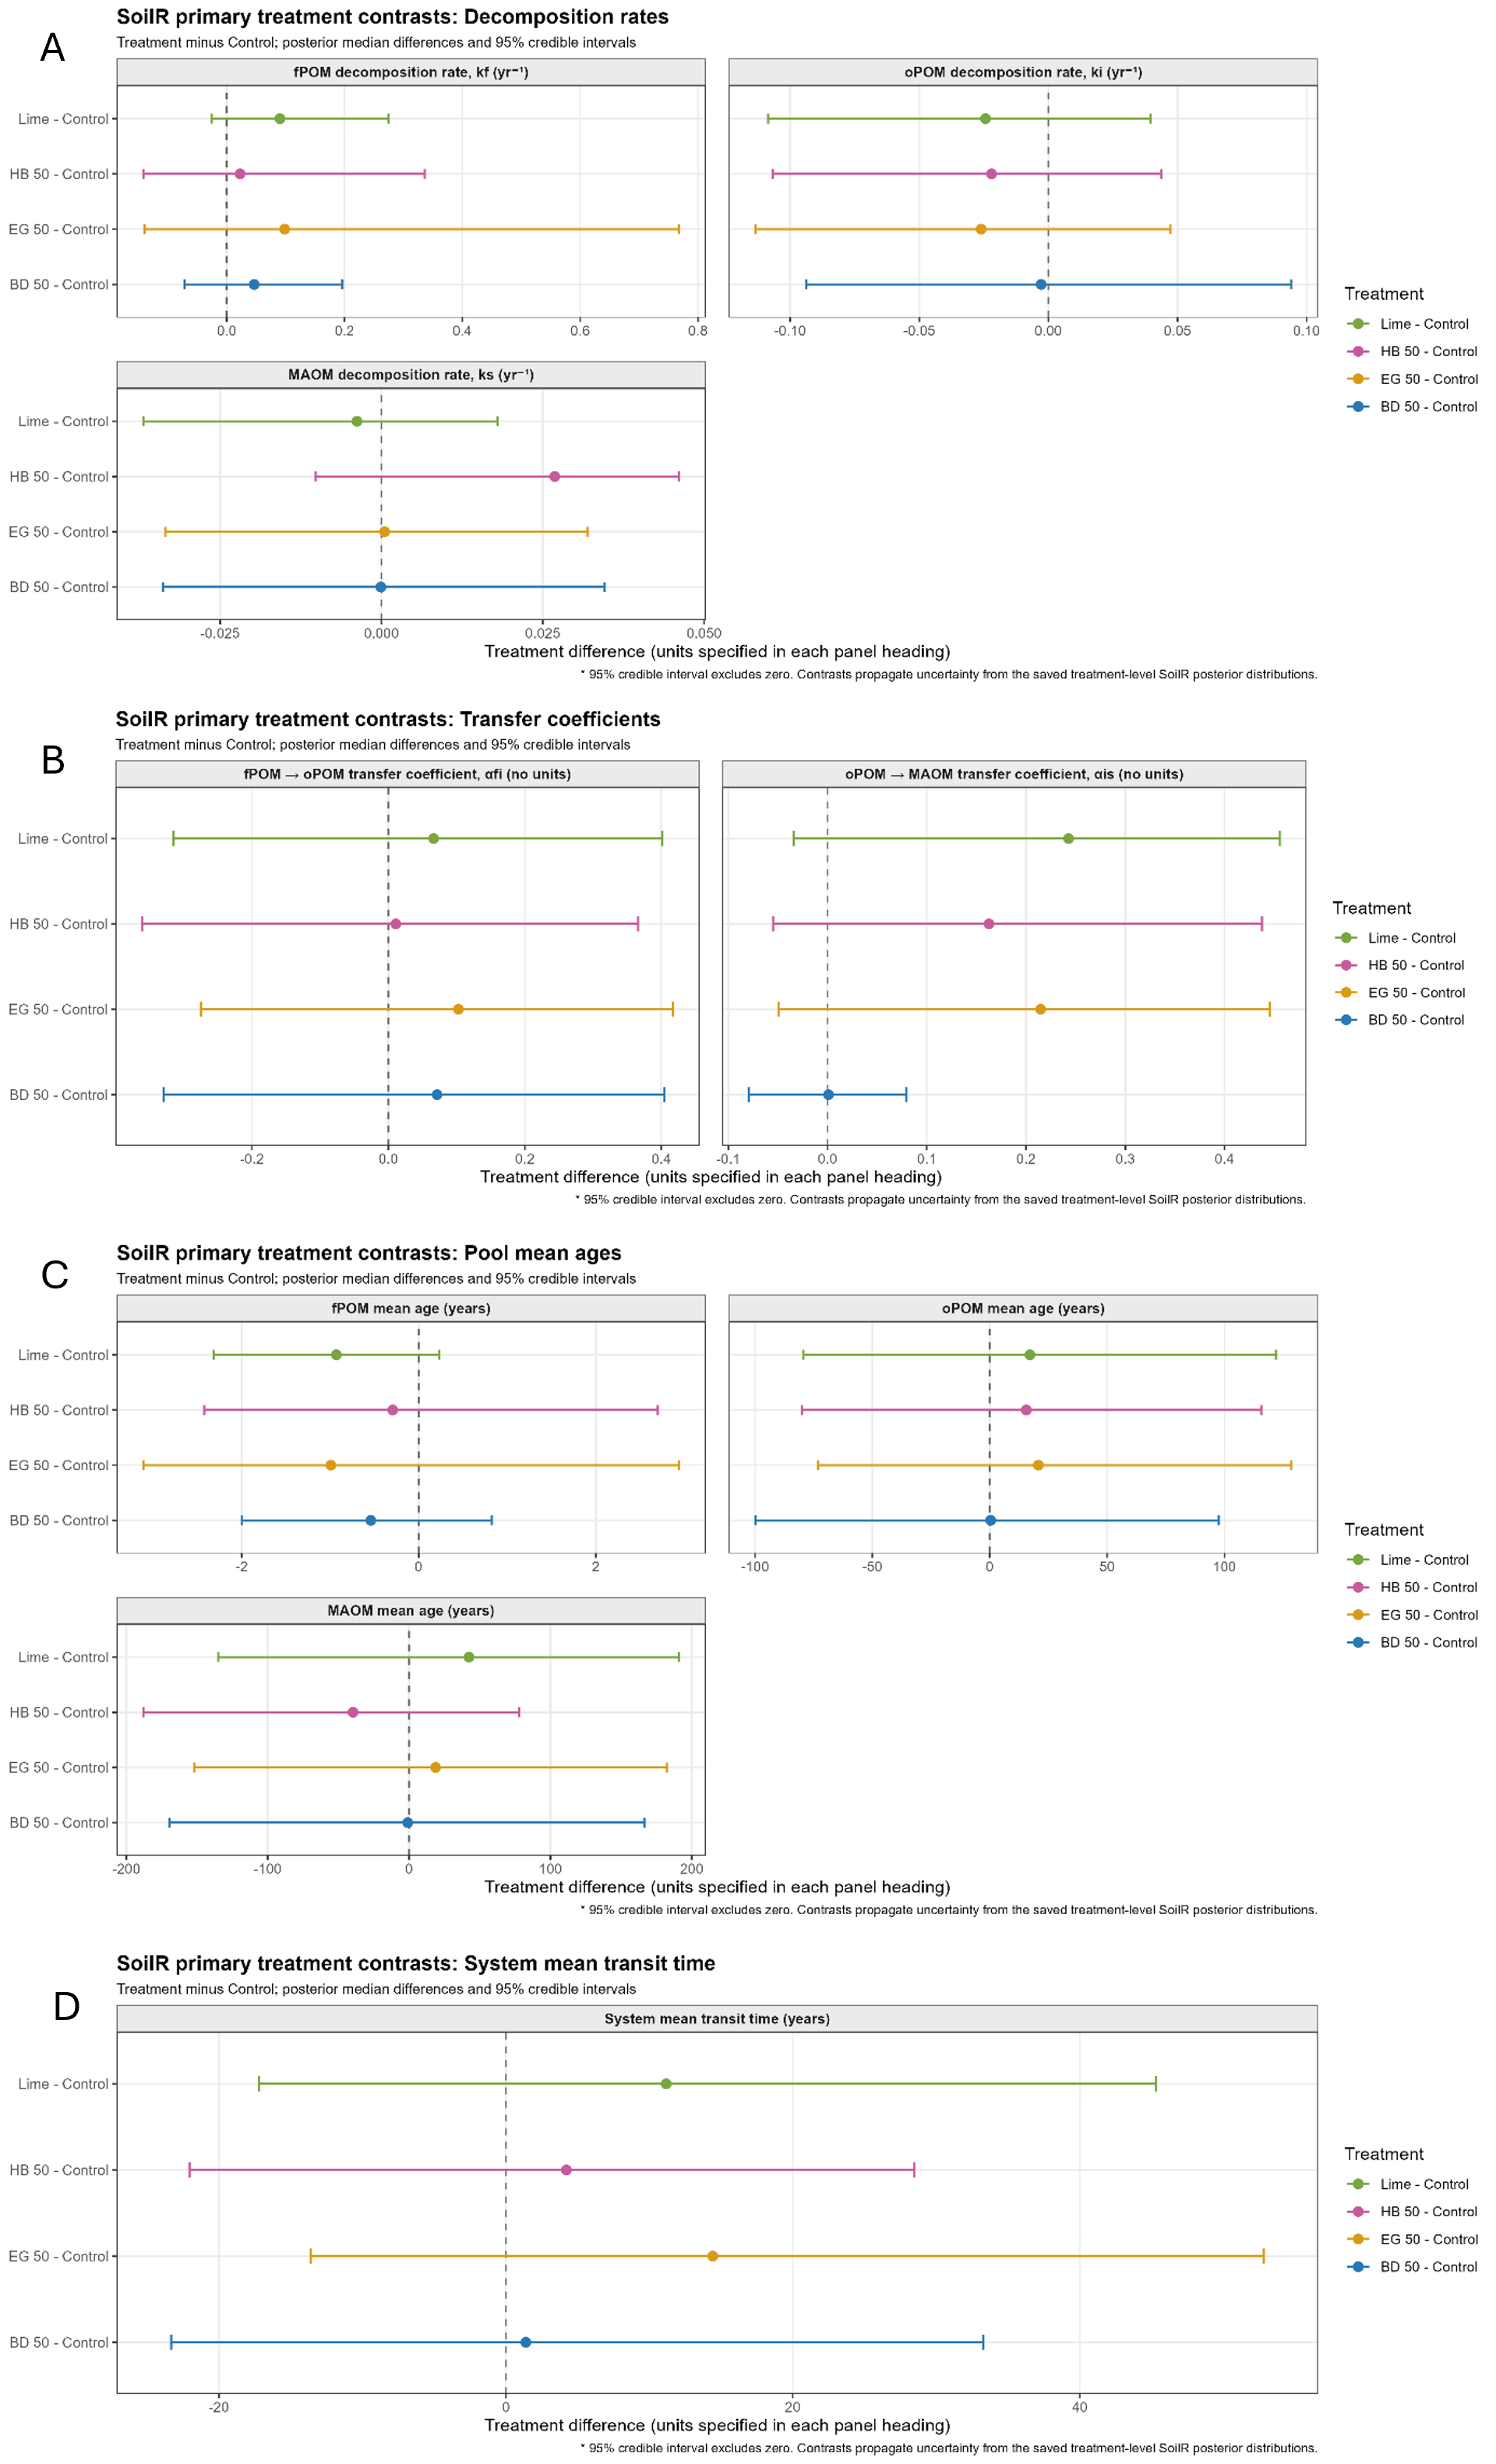
\includegraphics[width=0.8\textwidth]{figures/SoilRpars_comparison.png} 
    \caption{Posterior comparisons of three-pool SoilR compartmental model parameters—decomposition rate constants for free particulate ($k_f$), occluded particulate ($k_i$), and mineral-associated ($k_s$) organic matter (yr$^{-1}$), transfer coefficients from fPOM to oPOM ($\alpha_{fi}$) and oPOM to MAOM ($\alpha_{is}$), pool ages (yr), and whole-system carbon transit time (yr, time from fPOM input to respiratory loss)—between amended treatments and the unamended control (1,000 posterior draws per treatment after 20,000 burn-in iterations from 50,000 adaptive Metropolis MCMC steps).}
    \label{fig:SoilRpars_comparison}
\end{figure}

\newpage

\begin{figure}[htbp]
    \centering
    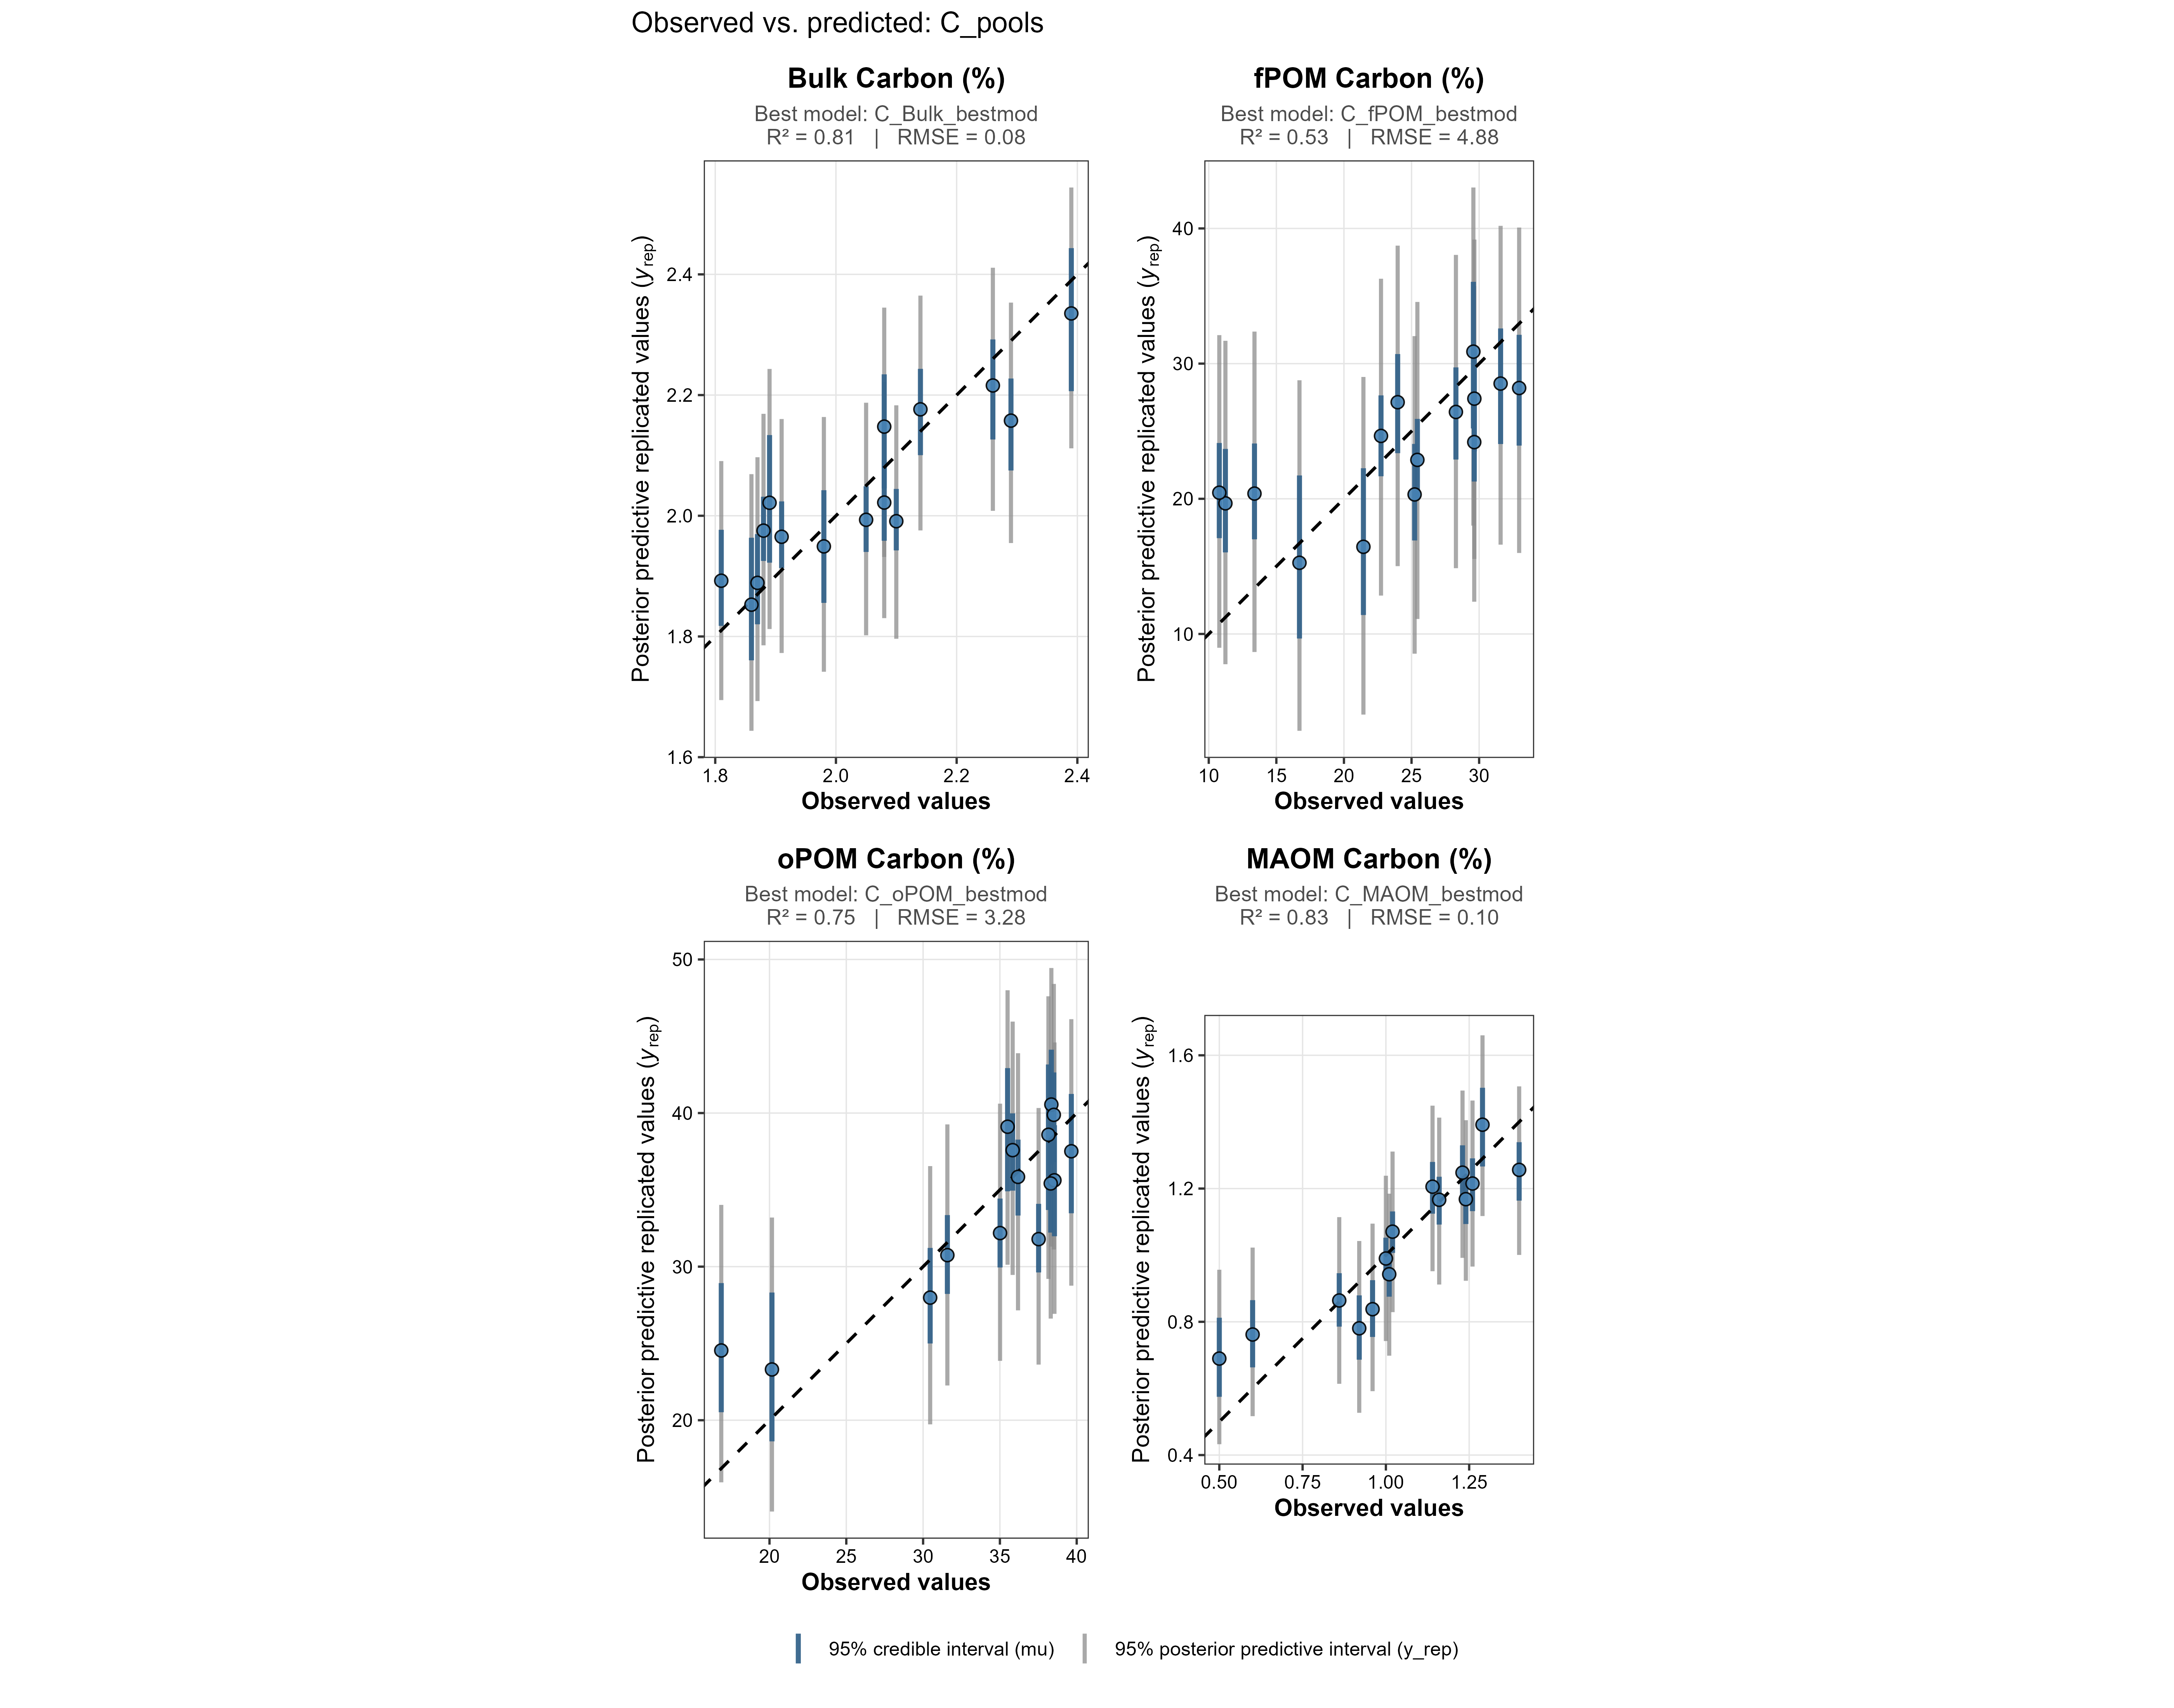
\includegraphics[width=1.2\textwidth]{figures/observed_vs_predicted_panel_C_pools.png} 
    \caption{Observed versus posterior predictive organic carbon concentrations across bulk soil and physical density fractions (fPOM, oPOM, and MAOM) from one-standard-error parsimonious Bayesian Gaussian models selected via projection predictive variable selection (projpred) and PSIS-LOO cross-validation on standardized ($z$-scored) geochemical and spectroscopic predictors (n = 15 plots).  }
\end{figure}

\newpage

\begin{figure}[htbp]
    \centering
    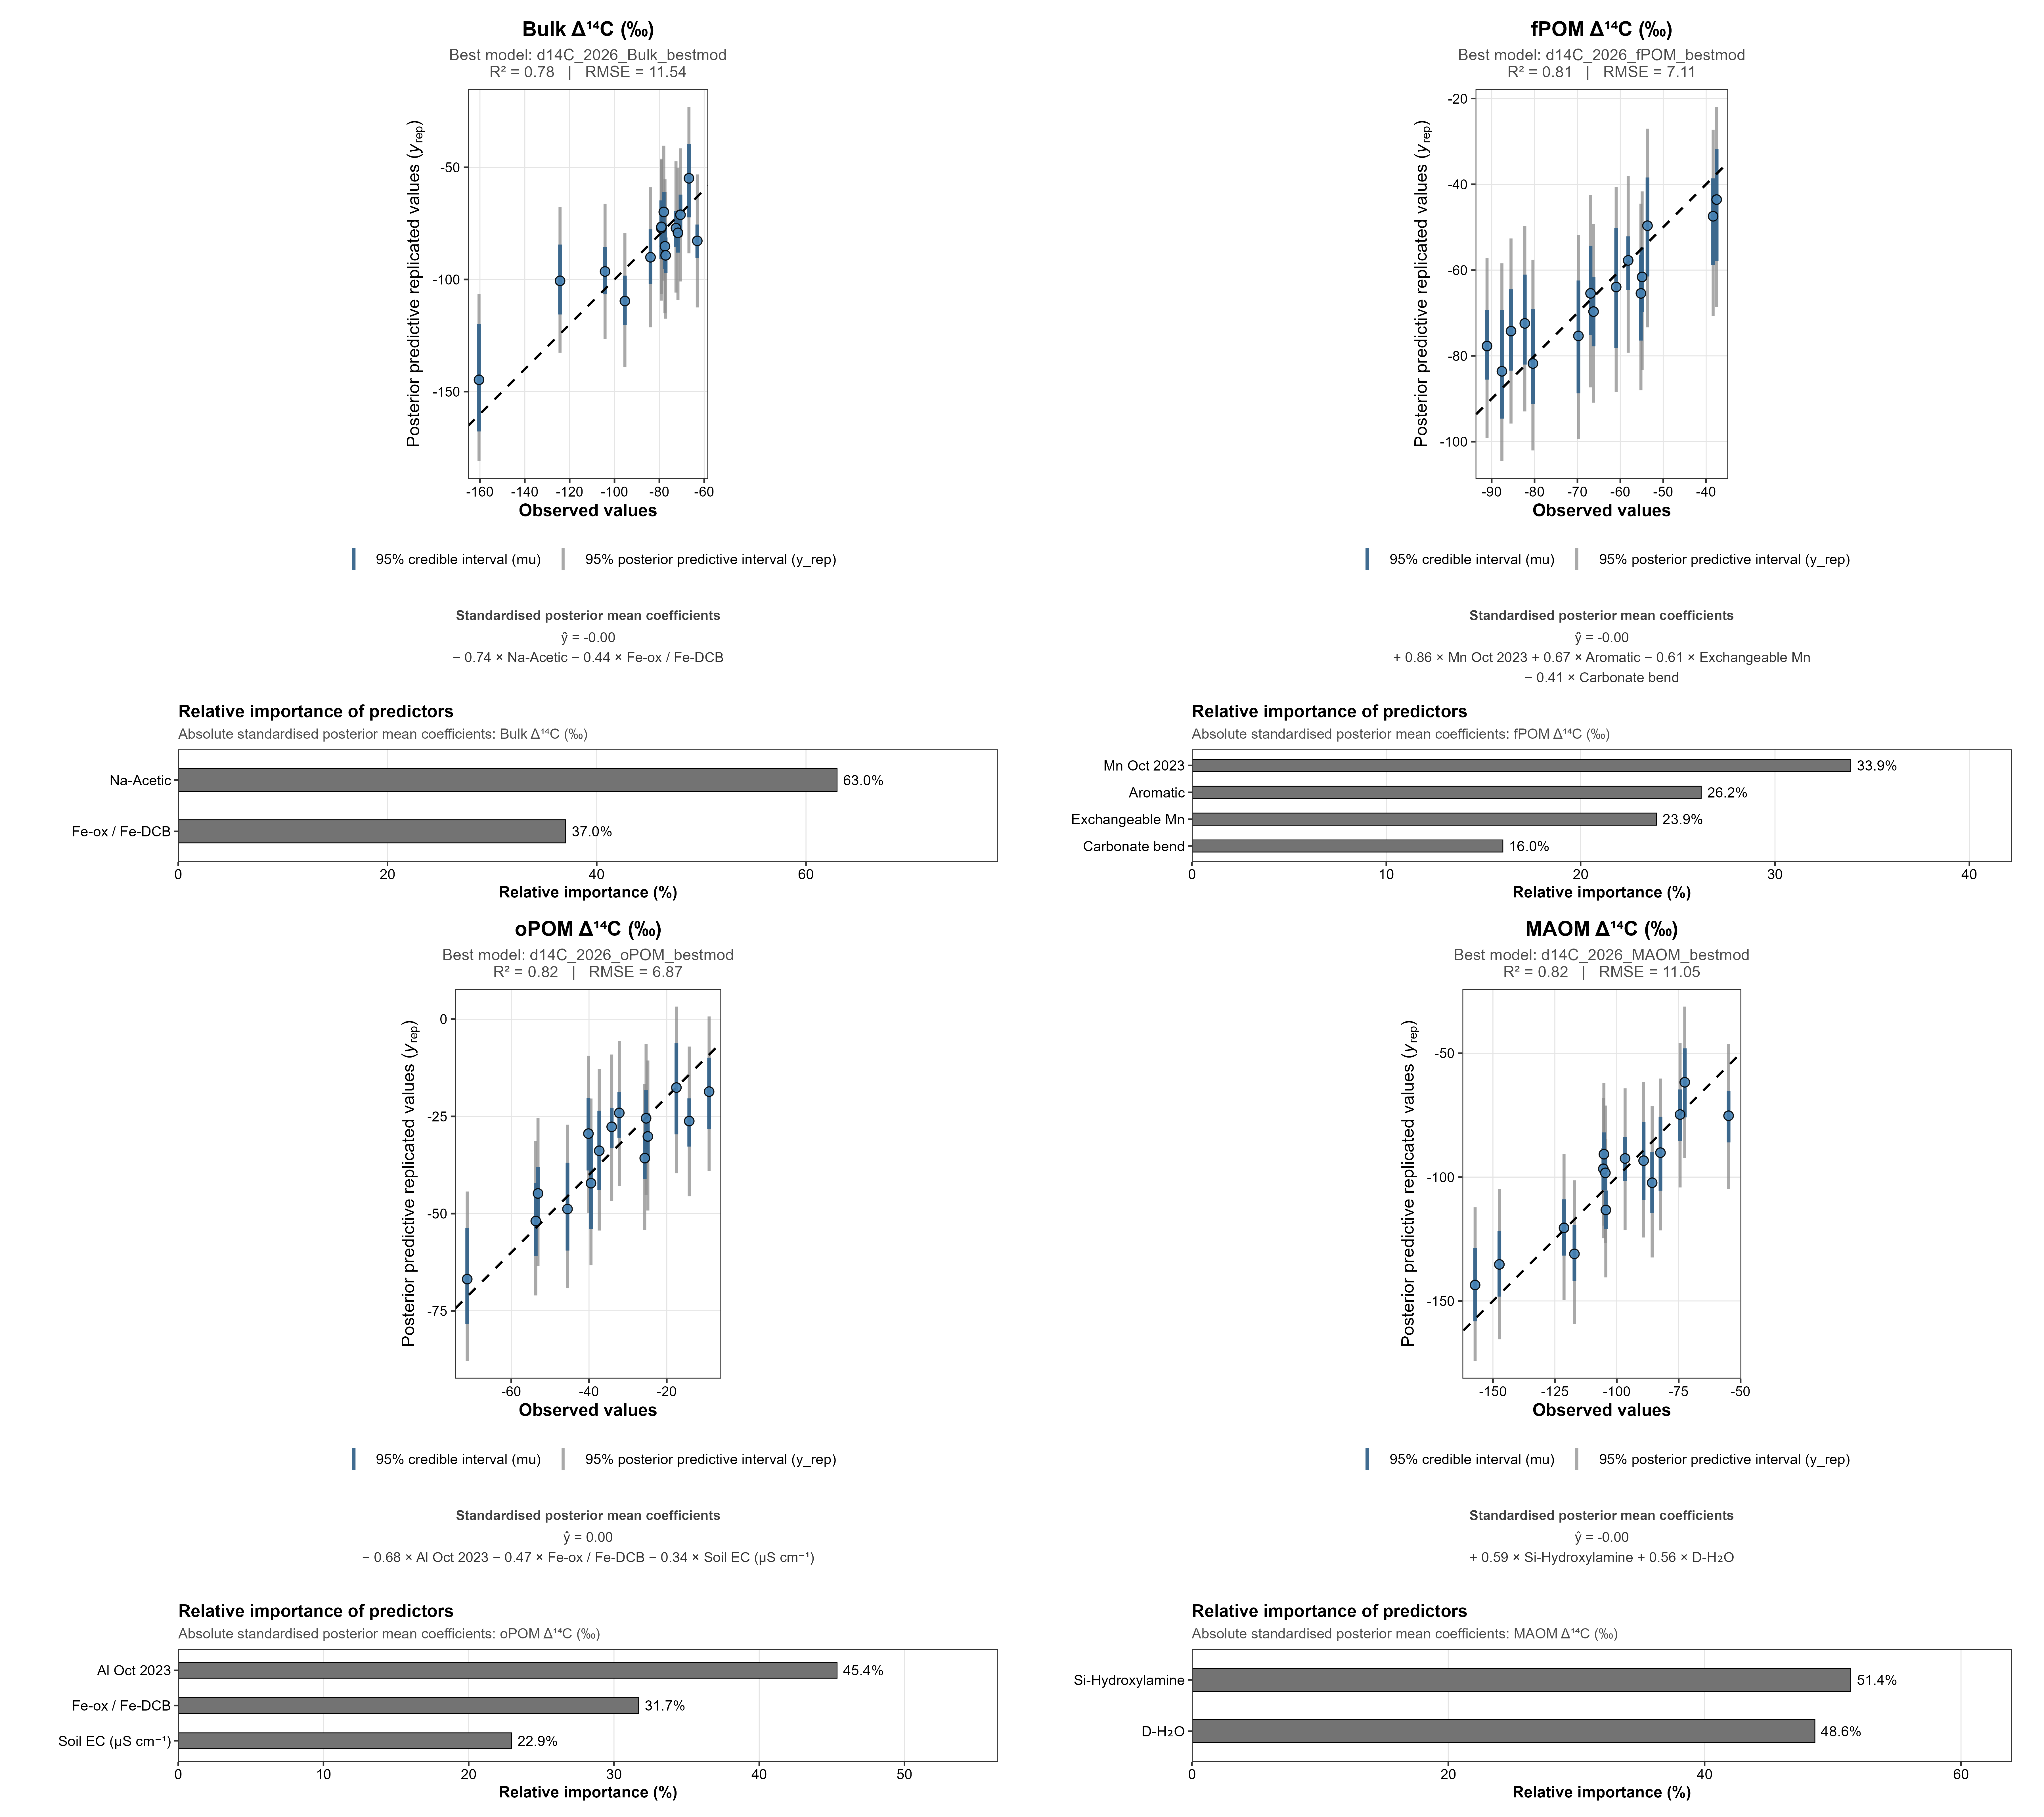
\includegraphics[width=1.2\textwidth]{figures/observed_vs_predicted_panel_d14C_pools.png} 
    \caption{Posterior Spearman rank correlations ($r$) between SoilR compartmental turnover/persistence parameters and soil geochemical or ATR-FTIR predictors, propagating parameter uncertainty across posterior draws. Predictors are shown where absolute median $\vert{}r\vert{} \ge 0.5$ for at least one parameter.}
\end{figure}

\newpage


  \begin{figure}[htbp]
    \centering
    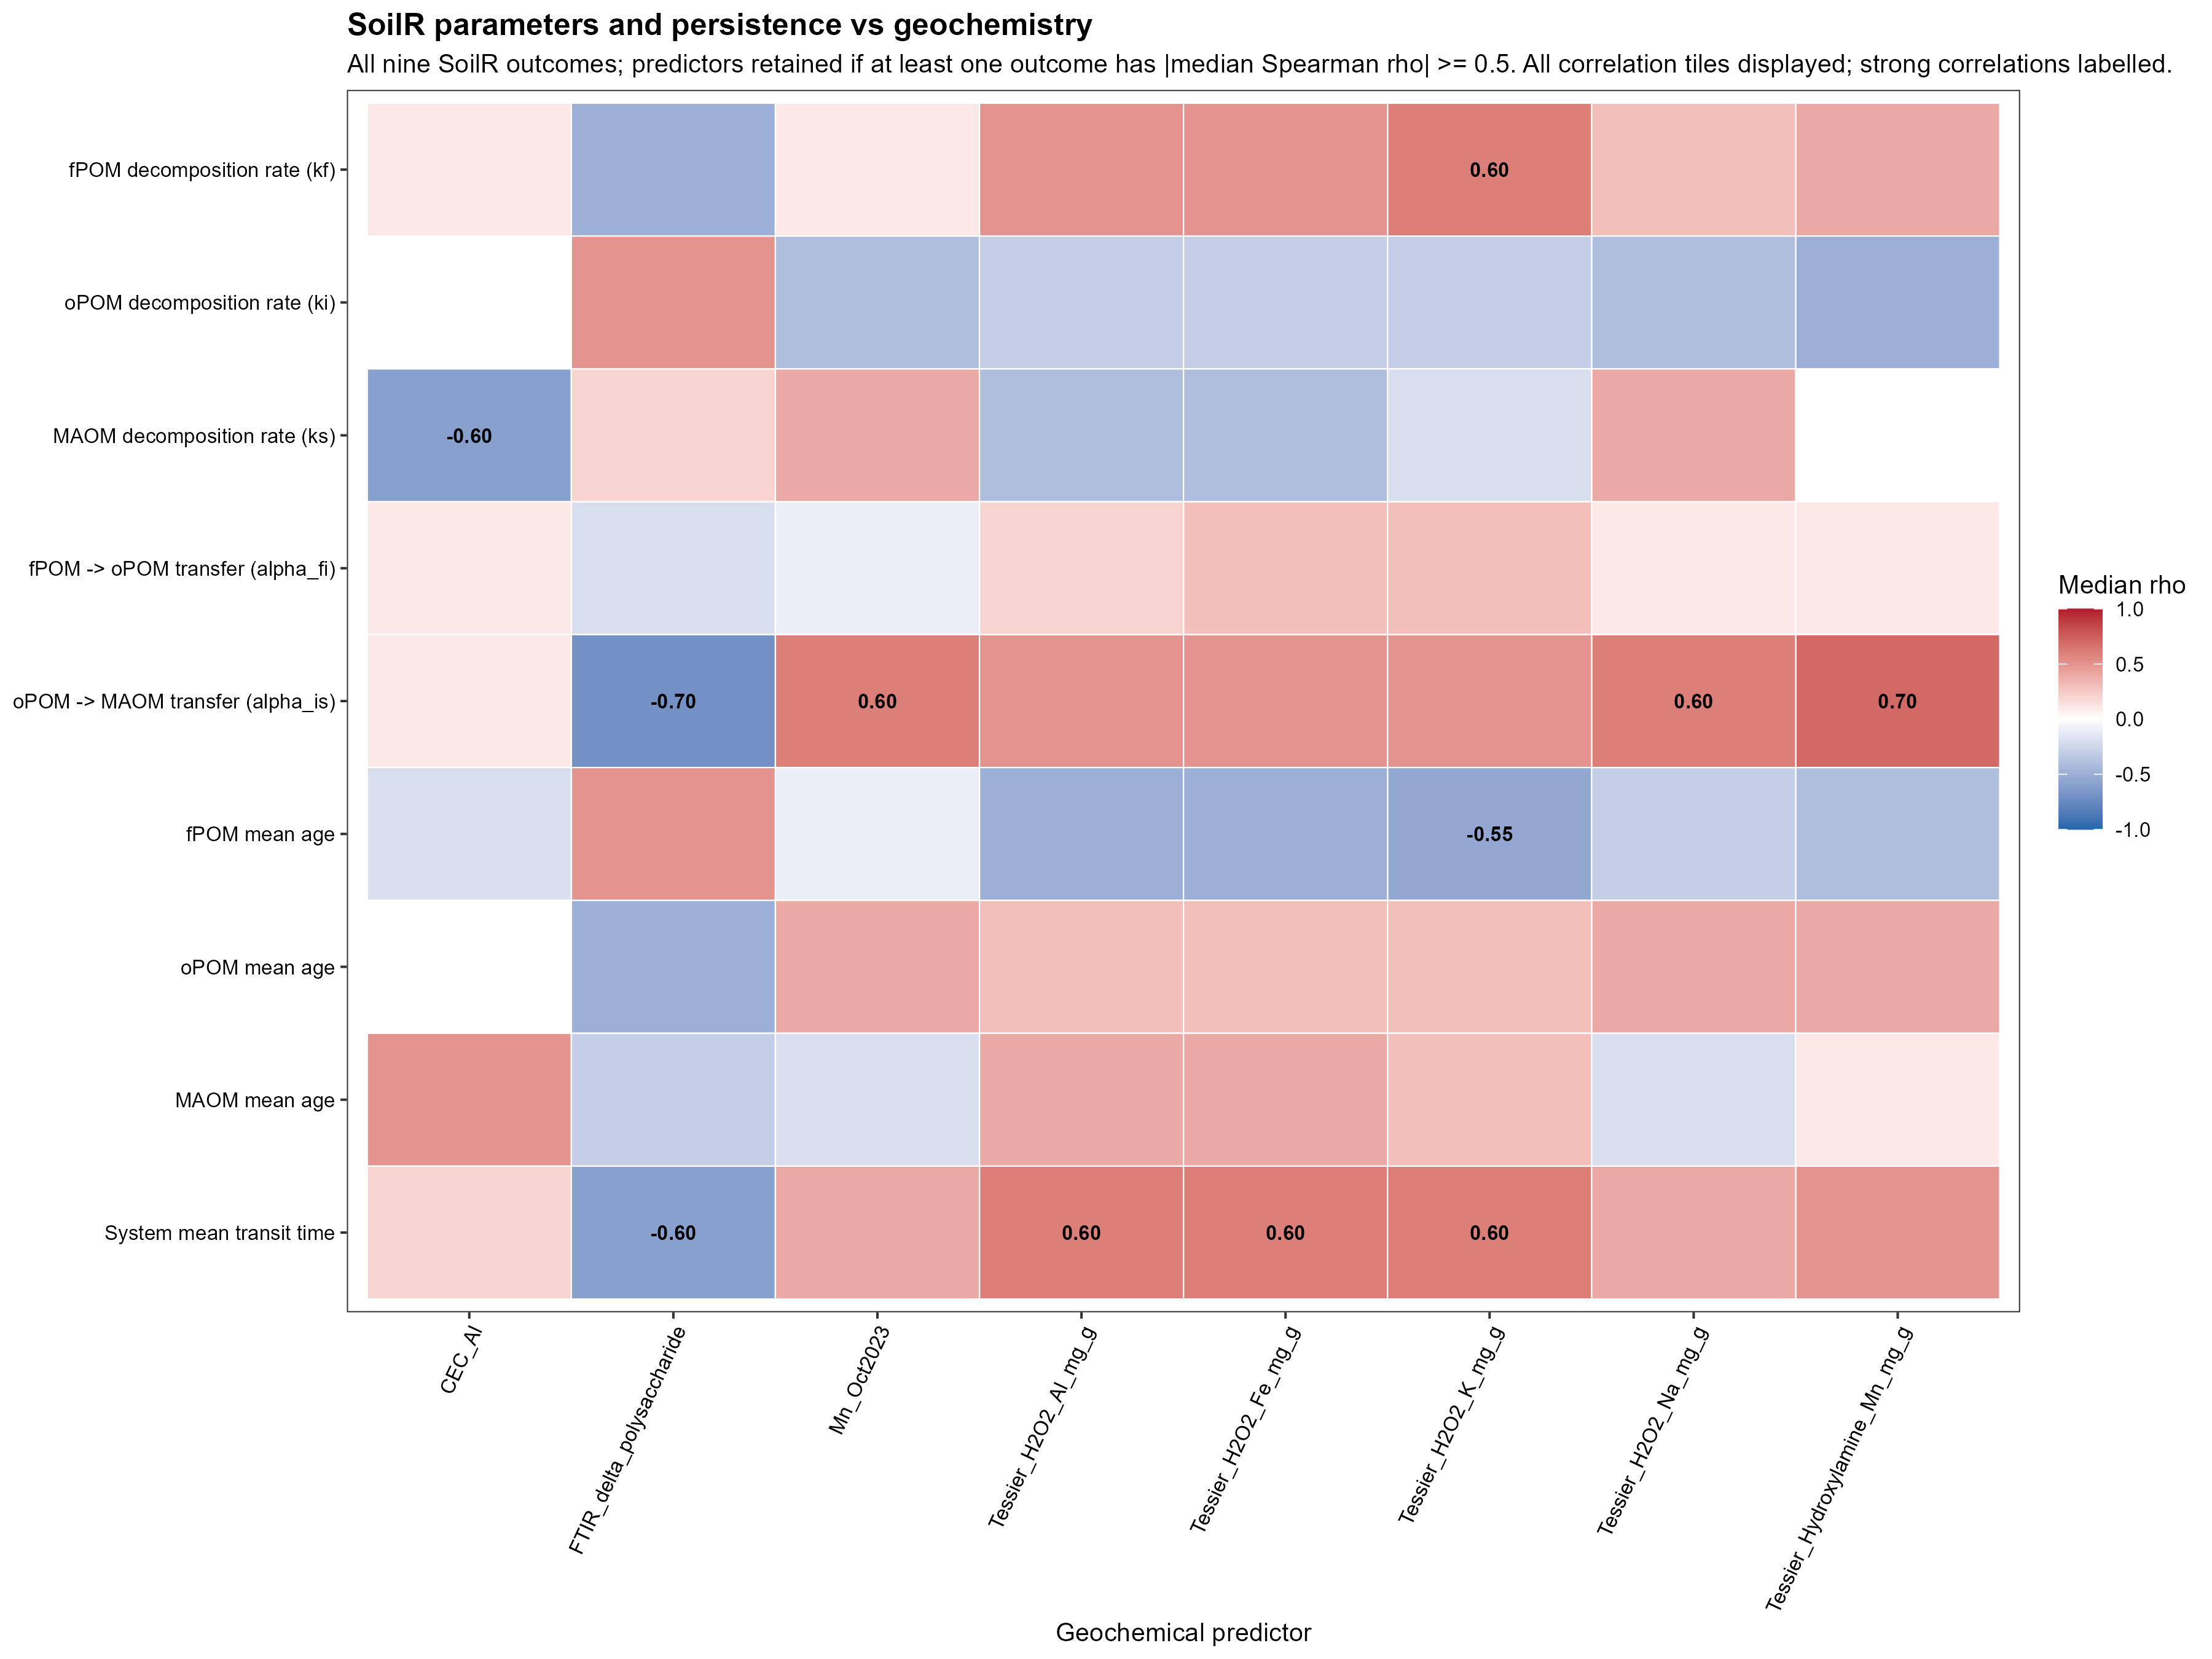
\includegraphics[width=1.0\textwidth]{figures/soilR_spearmancorr.png} 
    \caption{Spearman correlation between compartmental model-derived parameters (soil organic matter decomposition rates, transfer coefficients, soil organic matter pool ages and system transit time) and geochemical properties. Geochemical predictors are displayed only where the absolute median Spearman rho $\geq$ 0.5 for at least one parameter}
    \label{fig:soilR_spearmancorr}
\end{figure}

\newpage


% -----------------------------------------------------------------------------
% 10. REFERENCES
% -----------------------------------------------------------------------------

\bibliography{references}

% -----------------------------------------------------------------------------
% 11. SUPPLEMENTARY MATERIAL
% -----------------------------------------------------------------------------
\section{Supplementary Information}
\label{sec:si}

% Reset counters so numbering restarts at 1 (S1, S2, ...)
\setcounter{figure}{0}
\setcounter{table}{0}
\setcounter{equation}{0}

% Prepend 'S' to all counters globally
\renewcommand{\thesection}{S\arabic{section}}
\renewcommand{\thefigure}{S\arabic{figure}}
\renewcommand{\thetable}{S\arabic{table}}
\renewcommand{\theequation}{S\arabic{equation}}

% Configure cleveref labels
\crefname{section}{Section}{Sections}
\crefname{figure}{Fig.}{Figs.}
\crefname{table}{Table}{Tables}
\crefname{equation}{Eq.}{Eqs.}

\subsection{Supplementary Methods}
\label{sec:si_methods}
Add method descriptions if methods section in main text gets too long.

\subsection{Supplementary Tables}
\label{sec:si_tables}

\begin{landscape}
\begin{longtable}{lllrrrrr}
\caption{Posterior means, medians, and 95\% credible intervals (in standardized $z$-score and original measurement units) for soil physicochemical, cation, oxide, aggregate, and carbon/radiocarbon variables across treatments (17 responses $\times$ 5 treatments; filtered from geochem_means.csv, fitted in cmdstanr using a Student-t likelihood with $\nu = 4$.}\\
\label{tab:geochem_means_sub}\\
\toprule
Response & Treatment & Mean$_{\text{std}}$ & Med.$_{\text{std}}$ & CI95$_{\text{std}}$ & Mean$_{\text{orig}}$ & Med.$_{\text{orig}}$ & CI95$_{\text{orig}}$ \\
\midrule
\endfirsthead
\multicolumn{8}{c}{{\tablename\ \thetable{} -- continued from previous page}} \\
\toprule
Response & Treatment & Mean$_{\text{std}}$ & Med.$_{\text{std}}$ & CI95$_{\text{std}}$ & Mean$_{\text{orig}}$ & Med.$_{\text{orig}}$ & CI95$_{\text{orig}}$ \\
\midrule
\endhead
\midrule \multicolumn{8}{r}{{Continued on next page}} \\ \endfoot
\bottomrule \endlastfoot
soil\_pH & Control & -0.989 & -1.000 & [-1.84, -0.07] & 5.993 & 5.991 & [5.879, 6.115] \\
soil\_pH & Lime & 0.413 & 0.422 & [-0.45, 1.25] & 6.180 & 6.181 & [6.064, 6.291] \\
soil\_pH & HB 50 & 0.272 & 0.279 & [-0.61, 1.11] & 6.161 & 6.162 & [6.044, 6.273] \\
soil\_pH & EG 50 & -0.230 & -0.238 & [-1.17, 0.74] & 6.094 & 6.093 & [5.969, 6.223] \\
soil\_pH & BD 50 & 0.620 & 0.632 & [-0.22, 1.40] & 6.207 & 6.209 & [6.095, 6.312] \\
CEC\_K & Control & -0.305 & -0.306 & [-1.17, 0.58] & 0.173 & 0.172 & [0.123, 0.223] \\
CEC\_K & Lime & -0.267 & -0.283 & [-1.15, 0.69] & 0.175 & 0.174 & [0.124, 0.229] \\
CEC\_K & HB 50 & -0.470 & -0.473 & [-1.34, 0.44] & 0.163 & 0.163 & [0.113, 0.215] \\
CEC\_K & EG 50 & -0.071 & -0.075 & [-0.95, 0.80] & 0.186 & 0.186 & [0.136, 0.236] \\
CEC\_K & BD 50 & 1.082 & 1.110 & [0.05, 1.96] & 0.252 & 0.253 & [0.193, 0.302] \\
CEC\_Mg & Control & -0.664 & -0.677 & [-1.53, 0.31] & 0.744 & 0.742 & [0.599, 0.908] \\
CEC\_Mg & Lime & -0.310 & -0.316 & [-1.22, 0.63] & 0.804 & 0.803 & [0.652, 0.961] \\
CEC\_Mg & HB 50 & 0.947 & 0.963 & [-0.01, 1.81] & 1.015 & 1.017 & [0.855, 1.159] \\
CEC\_Mg & EG 50 & -0.118 & -0.124 & [-1.05, 0.85] & 0.836 & 0.835 & [0.680, 0.998] \\
CEC\_Mg & BD 50 & 0.128 & 0.135 & [-0.80, 1.03] & 0.877 & 0.879 & [0.722, 1.028] \\
CEC\_Na & Control & -0.486 & -0.492 & [-1.01, 0.06] & 0.030 & 0.030 & [0.019, 0.041] \\
CEC\_Na & Lime & -0.711 & -0.728 & [-1.17, -0.15] & 0.025 & 0.025 & [0.016, 0.037] \\
CEC\_Na & HB 50 & -0.409 & -0.417 & [-0.88, 0.12] & 0.032 & 0.031 & [0.022, 0.043] \\
CEC\_Na & EG 50 & 0.140 & 0.142 & [-0.36, 0.62] & 0.043 & 0.043 & [0.033, 0.053] \\
CEC\_Na & BD 50 & 0.982 & 0.924 & [0.42, 1.75] & 0.061 & 0.060 & [0.049, 0.077] \\
Si\_ox\_over\_DCB & Control & -0.717 & -0.725 & [-1.33, -0.06] & 0.233 & 0.230 & [-0.004, 0.486] \\
Si\_ox\_over\_DCB & Lime & -0.516 & -0.524 & [-1.14, 0.15] & 0.311 & 0.308 & [0.072, 0.568] \\
Si\_ox\_over\_DCB & HB 50 & -0.436 & -0.441 & [-1.06, 0.20] & 0.342 & 0.339 & [0.102, 0.586] \\
Si\_ox\_over\_DCB & EG 50 & 0.322 & 0.319 & [-0.36, 1.00] & 0.633 & 0.631 & [0.372, 0.893] \\
Si\_ox\_over\_DCB & BD 50 & 1.315 & 1.335 & [0.43, 2.08] & 1.014 & 1.022 & [0.674, 1.306] \\
Fe\_ox\_over\_Si\_ox & Control & 1.041 & 1.059 & [0.19, 1.81] & 8.479 & 8.537 & [5.673, 11.007] \\
Fe\_ox\_over\_Si\_ox & Lime & 0.430 & 0.436 & [-0.34, 1.17] & 6.465 & 6.485 & [3.922, 8.914] \\
Fe\_ox\_over\_Si\_ox & HB 50 & -0.059 & -0.063 & [-0.73, 0.65] & 4.850 & 4.840 & [2.638, 7.176] \\
Fe\_ox\_over\_Si\_ox & EG 50 & -0.609 & -0.618 & [-1.26, 0.11] & 3.040 & 3.008 & [0.888, 5.420] \\
Fe\_ox\_over\_Si\_ox & BD 50 & -0.885 & -0.896 & [-1.54, -0.16] & 2.131 & 2.092 & [-0.030, 4.533] \\
Al\_ox\_over\_Si\_ox & Control & 1.340 & 1.351 & [0.80, 1.81] & 17.106 & 17.167 & [14.204, 19.641] \\
Al\_ox\_over\_Si\_ox & Lime & 0.623 & 0.626 & [0.16, 1.07] & 13.268 & 13.287 & [10.814, 15.645] \\
Al\_ox\_over\_Si\_ox & HB 50 & -0.173 & -0.174 & [-0.63, 0.26] & 9.011 & 9.005 & [6.580, 11.309] \\
Al\_ox\_over\_Si\_ox & EG 50 & -0.653 & -0.658 & [-1.10, -0.18] & 6.443 & 6.416 & [4.060, 8.981] \\
Al\_ox\_over\_Si\_ox & BD 50 & -1.128 & -1.133 & [-1.56, -0.67] & 3.902 & 3.874 & [1.611, 6.361] \\
Tessier\_Acetic\_K\_mg\_g & Control & -0.476 & -0.479 & [-0.61, -0.31] & 0.003 & 0.003 & [-0.005, 0.013] \\
Tessier\_Acetic\_K\_mg\_g & Lime & -0.445 & -0.447 & [-0.59, -0.29] & 0.005 & 0.005 & [-0.003, 0.015] \\
Tessier\_Acetic\_K\_mg\_g & HB 50 & -0.389 & -0.389 & [-0.54, -0.23] & 0.009 & 0.009 & [-0.000, 0.018] \\
Tessier\_Acetic\_K\_mg\_g & EG 50 & -0.276 & -0.281 & [-0.42, -0.11] & 0.015 & 0.015 & [0.007, 0.025] \\
Tessier\_Acetic\_K\_mg\_g & BD 50 & 0.817 & 0.895 & [0.32, 1.27] & 0.081 & 0.085 & [0.051, 0.108] \\
Tessier\_Acetic\_Na\_mg\_g & Control & -0.582 & -0.592 & [-0.95, -0.14] & 0.005 & 0.004 & [-0.031, 0.046] \\
Tessier\_Acetic\_Na\_mg\_g & Lime & -0.579 & -0.590 & [-0.94, -0.15] & 0.005 & 0.004 & [-0.030, 0.046] \\
Tessier\_Acetic\_Na\_mg\_g & HB 50 & -0.378 & -0.386 & [-0.75, 0.05] & 0.024 & 0.023 & [-0.012, 0.064] \\
Tessier\_Acetic\_Na\_mg\_g & EG 50 & 0.023 & -0.000 & [-0.37, 0.48] & 0.062 & 0.060 & [0.024, 0.106] \\
Tessier\_Acetic\_Na\_mg\_g & BD 50 & 0.865 & 0.872 & [0.26, 1.64] & 0.143 & 0.143 & [0.085, 0.217] \\
Tessier\_Acetic\_Mg\_mg\_g & Control & -1.006 & -1.026 & [-1.64, -0.29] & 0.011 & 0.011 & [0.007, 0.017] \\
Tessier\_Acetic\_Mg\_mg\_g & Lime & -0.288 & -0.293 & [-0.94, 0.39] & 0.017 & 0.017 & [0.012, 0.022] \\
Tessier\_Acetic\_Mg\_mg\_g & HB 50 & 1.175 & 1.185 & [0.44, 1.87] & 0.028 & 0.028 & [0.022, 0.033] \\
Tessier\_Acetic\_Mg\_mg\_g & EG 50 & -0.354 & -0.356 & [-1.05, 0.35] & 0.016 & 0.016 & [0.011, 0.022] \\
Tessier\_Acetic\_Mg\_mg\_g & BD 50 & 0.421 & 0.423 & [-0.24, 1.06] & 0.022 & 0.022 & [0.017, 0.027] \\
Tessier\_H2O2\_Fe\_mg\_g & Control & -1.002 & -1.023 & [-1.86, -0.07] & 0.061 & 0.061 & [0.038, 0.087] \\
Tessier\_H2O2\_Fe\_mg\_g & Lime & 0.469 & 0.479 & [-0.46, 1.37] & 0.102 & 0.102 & [0.076, 0.127] \\
Tessier\_H2O2\_Fe\_mg\_g & HB 50 & -0.017 & -0.017 & [-0.90, 0.84] & 0.089 & 0.089 & [0.064, 0.112] \\
Tessier\_H2O2\_Fe\_mg\_g & EG 50 & 0.309 & 0.312 & [-0.62, 1.23] & 0.098 & 0.098 & [0.072, 0.123] \\
Tessier\_H2O2\_Fe\_mg\_g & BD 50 & 0.330 & 0.339 & [-0.71, 1.31] & 0.098 & 0.098 & [0.069, 0.125] \\
Tessier\_H2O2\_Al\_mg\_g & Control & -0.991 & -1.003 & [-1.86, -0.02] & 0.035 & 0.035 & [0.019, 0.054] \\
Tessier\_H2O2\_Al\_mg\_g & Lime & 0.433 & 0.438 & [-0.54, 1.37] & 0.062 & 0.062 & [0.044, 0.080] \\
Tessier\_H2O2\_Al\_mg\_g & HB 50 & 0.056 & 0.053 & [-0.89, 0.96] & 0.055 & 0.055 & [0.037, 0.072] \\
Tessier\_H2O2\_Al\_mg\_g & EG 50 & 0.392 & 0.401 & [-0.56, 1.33] & 0.062 & 0.062 & [0.044, 0.079] \\
Tessier\_H2O2\_Al\_mg\_g & BD 50 & 0.061 & 0.064 & [-0.85, 0.96] & 0.055 & 0.055 & [0.038, 0.072] \\
Tessier\_H2O2\_Si\_mg\_g & Control & -1.075 & -1.092 & [-1.91, -0.15] & 0.057 & 0.057 & [0.038, 0.079] \\
Tessier\_H2O2\_Si\_mg\_g & Lime & 0.423 & 0.440 & [-0.51, 1.27] & 0.093 & 0.093 & [0.071, 0.113] \\
Tessier\_H2O2\_Si\_mg\_g & HB 50 & 0.129 & 0.129 & [-0.78, 1.04] & 0.086 & 0.086 & [0.064, 0.107] \\
Tessier\_H2O2\_Si\_mg\_g & EG 50 & 0.100 & 0.101 & [-0.78, 0.97] & 0.085 & 0.085 & [0.064, 0.105] \\
Tessier\_H2O2\_Si\_mg\_g & BD 50 & 0.450 & 0.464 & [-0.55, 1.37] & 0.093 & 0.094 & [0.070, 0.115] \\
Tessier\_Hydroxylamine\_Fe\_mg\_g & Control & -0.971 & -0.991 & [-1.83, -0.00] & 1.000 & 0.994 & [0.739, 1.295] \\
Tessier\_Hydroxylamine\_Fe\_mg\_g & Lime & 0.282 & 0.288 & [-0.66, 1.16] & 1.382 & 1.384 & [1.096, 1.649] \\
Tessier\_Hydroxylamine\_Fe\_mg\_g & HB 50 & 0.427 & 0.433 & [-0.51, 1.31] & 1.426 & 1.428 & [1.141, 1.696] \\
Tessier\_Hydroxylamine\_Fe\_mg\_g & EG 50 & -0.080 & -0.080 & [-0.98, 0.85] & 1.272 & 1.272 & [0.996, 1.554] \\
Tessier\_Hydroxylamine\_Fe\_mg\_g & BD 50 & 0.276 & 0.276 & [-0.75, 1.30] & 1.380 & 1.380 & [1.068, 1.691] \\
Tessier\_Hydroxylamine\_Si\_mg\_g & Control & -1.044 & -1.060 & [-1.90, -0.08] & 0.558 & 0.554 & [0.367, 0.773] \\
Tessier\_Hydroxylamine\_Si\_mg\_g & Lime & 0.216 & 0.217 & [-0.68, 1.10] & 0.838 & 0.839 & [0.640, 1.036] \\
Tessier\_Hydroxylamine\_Si\_mg\_g & HB 50 & 0.574 & 0.583 & [-0.38, 1.48] & 0.918 & 0.920 & [0.707, 1.120] \\
Tessier\_Hydroxylamine\_Si\_mg\_g & EG 50 & -0.098 & -0.100 & [-0.94, 0.75] & 0.768 & 0.768 & [0.581, 0.957] \\
Tessier\_Hydroxylamine\_Si\_mg\_g & BD 50 & 0.335 & 0.332 & [-0.58, 1.25] & 0.865 & 0.864 & [0.661, 1.068] \\
D\_oxalate\_over\_h2o & Control & -0.789 & -0.805 & [-1.60, 0.07] & 1.046 & 1.046 & [1.033, 1.060] \\
D\_oxalate\_over\_h2o & Lime & 0.905 & 0.913 & [-0.00, 1.77] & 1.073 & 1.073 & [1.059, 1.087] \\
D\_oxalate\_over\_h2o & HB 50 & 0.411 & 0.408 & [-0.43, 1.25] & 1.065 & 1.065 & [1.052, 1.079] \\
D\_oxalate\_over\_h2o & EG 50 & -0.444 & -0.451 & [-1.28, 0.43] & 1.052 & 1.051 & [1.038, 1.065] \\
D\_oxalate\_over\_h2o & BD 50 & -0.154 & -0.157 & [-0.99, 0.70] & 1.056 & 1.056 & [1.043, 1.070] \\
C\_fPOM & Control & -0.752 & -0.763 & [-1.66, 0.21] & 17.954 & 17.873 & [11.270, 25.034] \\
C\_fPOM & Lime & -0.126 & -0.134 & [-1.10, 0.87] & 22.577 & 22.518 & [15.382, 29.928] \\
C\_fPOM & HB 50 & 0.676 & 0.692 & [-0.24, 1.52] & 28.498 & 28.614 & [21.740, 34.750] \\
C\_fPOM & EG 50 & -0.199 & -0.198 & [-1.11, 0.69] & 22.036 & 22.047 & [15.290, 28.631] \\
C\_fPOM & BD 50 & 0.482 & 0.498 & [-0.44, 1.38] & 27.066 & 27.184 & [20.259, 33.669] \\
\end{longtable}

\newpage

\begin{longtable}{llrrrrrl}
\caption{Supported Bayesian treatment-minus-control contrasts (Sig_Flag = *; 30 contrasts filtered from geochem_tmt_comparison.csv) in standardized and original units, with 95\% credible intervals and posterior exceedance probabilities $P(T_1 > T_2)$ computed from 10,000 posterior difference draws.}\\
\toprule
Response & Comparison & Diff.$_{\text{std}}$ & CI95$_{\text{std}}$ & Diff.$_{\text{orig}}$ & CI95$_{\text{orig}}$ & $P(T_1 > T_2)$ & Sig \\
\midrule
\endfirsthead
\multicolumn{8}{c}{{\tablename\ \thetable{} -- continued from previous page}} \\
\toprule
Response & Comparison & Diff.$_{\text{std}}$ & CI95$_{\text{std}}$ & Diff.$_{\text{orig}}$ & CI95$_{\text{orig}}$ & $P(T_1 > T_2)$ & Sig \\
\midrule
\endhead
\midrule \multicolumn{8}{r}{{Continued on next page}} \\ \endfoot
\bottomrule \endlastfoot
soil\_pH & Lime minus Control & 1.401 & [0.14, 2.57] & 0.187 & [0.018, 0.343] & 0.982 & * \\
soil\_pH & HB 50 minus Control & 1.261 & [0.00, 2.44] & 0.168 & [0.000, 0.326] & 0.975 & * \\
soil\_pH & BD 50 minus Control & 1.608 & [0.36, 2.75] & 0.215 & [0.047, 0.368] & 0.992 & * \\
CEC\_K & BD 50 minus Control & 1.388 & [0.05, 2.61] & 0.079 & [0.003, 0.149] & 0.978 & * \\
CEC\_Mg & HB 50 minus Control & 1.611 & [0.20, 2.84] & 0.270 & [0.033, 0.476] & 0.985 & * \\
CEC\_Na & BD 50 minus Control & 1.468 & [0.69, 2.42] & 0.031 & [0.014, 0.051] & 0.999 & * \\
Si\_ox\_over\_DCB & EG 50 minus Control & 1.039 & [0.05, 1.94] & 0.399 & [0.020, 0.746] & 0.980 & * \\
Si\_ox\_over\_DCB & BD 50 minus Control & 2.033 & [0.88, 3.03] & 0.781 & [0.339, 1.162] & 0.998 & * \\
Fe\_ox\_over\_Si\_ox & HB 50 minus Control & -1.101 & [-2.11, -0.01] & -3.628 & [-6.970, -0.048] & 0.024 & * \\
Fe\_ox\_over\_Si\_ox & EG 50 minus Control & -1.650 & [-2.66, -0.53] & -5.439 & [-8.776, -1.744] & 0.004 & * \\
Fe\_ox\_over\_Si\_ox & BD 50 minus Control & -1.926 & [-2.94, -0.79] & -6.348 & [-9.681, -2.606] & 0.002 & * \\
Al\_ox\_over\_Si\_ox & Lime minus Control & -0.717 & [-1.36, -0.01] & -3.838 & [-7.296, -0.071] & 0.023 & * \\
Al\_ox\_over\_Si\_ox & HB 50 minus Control & -1.513 & [-2.14, -0.79] & -8.096 & [-11.475, -4.244] & 0.000 & * \\
Al\_ox\_over\_Si\_ox & EG 50 minus Control & -1.993 & [-2.63, -1.28] & -10.663 & [-14.081, -6.831] & 0.000 & * \\
Al\_ox\_over\_Si\_ox & BD 50 minus Control & -2.468 & [-3.11, -1.73] & -13.205 & [-16.655, -9.257] & 0.000 & * \\
Tessier\_Acetic\_K\_mg\_g & BD 50 minus Control & 1.293 & [0.78, 1.78] & 0.077 & [0.047, 0.106] & 1.000 & * \\
Tessier\_Acetic\_Na\_mg\_g & EG 50 minus Control & 0.604 & [0.02, 1.19] & 0.058 & [0.002, 0.114] & 0.977 & * \\
Tessier\_Acetic\_Na\_mg\_g & BD 50 minus Control & 1.447 & [0.76, 2.33] & 0.138 & [0.072, 0.223] & 1.000 & * \\
Tessier\_Acetic\_Mg\_mg\_g & HB 50 minus Control & 2.181 & [1.10, 3.12] & 0.016 & [0.008, 0.023] & 0.999 & * \\
Tessier\_Acetic\_Mg\_mg\_g & BD 50 minus Control & 1.426 & [0.41, 2.31] & 0.011 & [0.003, 0.017] & 0.995 & * \\
Tessier\_H2O2\_Fe\_mg\_g & Lime minus Control & 1.471 & [0.13, 2.68] & 0.040 & [0.004, 0.074] & 0.984 & * \\
Tessier\_H2O2\_Al\_mg\_g & Lime minus Control & 1.424 & [0.06, 2.72] & 0.027 & [0.001, 0.052] & 0.978 & * \\
Tessier\_H2O2\_Al\_mg\_g & EG 50 minus Control & 1.383 & [0.04, 2.62] & 0.026 & [0.001, 0.050] & 0.978 & * \\
Tessier\_H2O2\_Si\_mg\_g & Lime minus Control & 1.498 & [0.16, 2.67] & 0.035 & [0.004, 0.063] & 0.984 & * \\
Tessier\_H2O2\_Si\_mg\_g & BD 50 minus Control & 1.526 & [0.12, 2.78] & 0.036 & [0.003, 0.065] & 0.984 & * \\
Tessier\_Hydroxylamine\_Fe\_mg\_g & HB 50 minus Control & 1.399 & [0.04, 2.63] & 0.426 & [0.012, 0.803] & 0.978 & * \\
Tessier\_Hydroxylamine\_Si\_mg\_g & HB 50 minus Control & 1.618 & [0.28, 2.85] & 0.361 & [0.062, 0.634] & 0.988 & * \\
Tessier\_Hydroxylamine\_Si\_mg\_g & BD 50 minus Control & 1.379 & [0.07, 2.60] & 0.307 & [0.016, 0.579] & 0.979 & * \\
D\_oxalate\_over\_h2o & Lime minus Control & 1.694 & [0.41, 2.84] & 0.027 & [0.007, 0.045] & 0.994 & * \\
C\_fPOM & HB 50 minus Control & 1.428 & [0.07, 2.66] & 10.543 & [0.492, 19.655] & 0.979 & * \\
\end{longtable}

\newpage

\begin{longtable}{llrrrrrr}
\caption{Posterior summary statistics (mean, median, SD, and 95\% credible interval) of SoilR three-pool compartmental parameters—decomposition rates ($k_f, k_i, k_s$), transfer coefficients ($\alpha_{fi}, \alpha_{is}$), pool ages, and whole-system transit time—from SoilRpars_means.csv ($n_{\text{draws}} = 1,000$ post-burn-in draws per treatment).}\\
\label{tab:soilr_means}\\
\toprule
Treatment & Response & Mean & Median & SD & 95\% CI Low & 95\% CI High \\
\midrule
\endfirsthead
\multicolumn{7}{c}{{\tablename\ \thetable{} -- continued from previous page}} \\
\toprule
Treatment & Response & Mean & Median & SD & 95\% CI Low & 95\% CI High \\
\midrule
\endhead
\midrule \multicolumn{7}{r}{{Continued on next page}} \\ \endfoot
\bottomrule \endlastfoot
Control & MAOM\_age & 130.635 & 116.200 & 59.267 & 50.990 & 251.466 \\
Control & alpha\_fi & 0.239 & 0.232 & 0.137 & 0.018 & 0.483 \\
Control & alpha\_is & 0.051 & 0.052 & 0.029 & 0.002 & 0.098 \\
Control & fPOM\_age & 3.622 & 3.587 & 0.502 & 2.679 & 4.705 \\
Control & kf & 0.278 & 0.275 & 0.038 & 0.211 & 0.365 \\
Control & ki & 0.056 & 0.050 & 0.034 & 0.007 & 0.133 \\
Control & ks & 0.015 & 0.012 & 0.012 & 0.001 & 0.043 \\
Control & oPOM\_age & 33.697 & 23.518 & 28.059 & 11.298 & 128.177 \\
Control & system\_transit\_time & 11.216 & 8.960 & 8.005 & 3.954 & 35.736 \\
Lime & MAOM\_age & 168.819 & 168.305 & 61.319 & 62.477 & 278.782 \\
Lime & alpha\_fi & 0.299 & 0.318 & 0.131 & 0.034 & 0.487 \\
Lime & alpha\_is & 0.283 & 0.297 & 0.140 & 0.022 & 0.489 \\
Lime & fPOM\_age & 2.654 & 2.720 & 0.405 & 1.739 & 3.384 \\
Lime & kf & 0.377 & 0.360 & 0.062 & 0.291 & 0.547 \\
Lime & ki & 0.028 & 0.025 & 0.018 & 0.006 & 0.068 \\
Lime & ks & 0.009 & 0.008 & 0.007 & 0.001 & 0.026 \\
Lime & oPOM\_age & 55.257 & 42.392 & 35.491 & 17.206 & 145.881 \\
Lime & system\_transit\_time & 23.748 & 21.182 & 12.781 & 4.812 & 57.662 \\
HB 50 & MAOM\_age & 81.459 & 70.092 & 34.640 & 43.710 & 168.119 \\
HB 50 & alpha\_fi & 0.248 & 0.250 & 0.133 & 0.018 & 0.477 \\
HB 50 & alpha\_is & 0.224 & 0.212 & 0.140 & 0.009 & 0.480 \\
HB 50 & fPOM\_age & 3.411 & 3.325 & 1.215 & 1.550 & 6.090 \\
HB 50 & kf & 0.325 & 0.296 & 0.117 & 0.163 & 0.607 \\
HB 50 & ki & 0.030 & 0.026 & 0.019 & 0.006 & 0.077 \\
HB 50 & ks & 0.040 & 0.042 & 0.009 & 0.016 & 0.050 \\
HB 50 & oPOM\_age & 53.725 & 42.888 & 33.598 & 17.649 & 139.231 \\
HB 50 & system\_transit\_time & 15.643 & 13.353 & 8.517 & 4.649 & 38.438 \\
EG 50 & MAOM\_age & 148.993 & 140.875 & 62.102 & 56.644 & 276.120 \\
EG 50 & alpha\_fi & 0.338 & 0.361 & 0.118 & 0.078 & 0.492 \\
EG 50 & alpha\_is & 0.256 & 0.257 & 0.146 & 0.017 & 0.486 \\
EG 50 & fPOM\_age & 2.912 & 2.711 & 1.076 & 1.333 & 5.502 \\
EG 50 & kf & 0.440 & 0.371 & 0.207 & 0.149 & 1.045 \\
EG 50 & ki & 0.027 & 0.023 & 0.018 & 0.006 & 0.074 \\
EG 50 & ks & 0.015 & 0.012 & 0.011 & 0.001 & 0.042 \\
EG 50 & oPOM\_age & 60.875 & 44.504 & 40.297 & 18.034 & 158.097 \\
EG 50 & system\_transit\_time & 22.976 & 18.887 & 13.550 & 6.238 & 58.149 \\
BD 50 & MAOM\_age & 129.066 & 115.635 & 56.103 & 51.842 & 242.193 \\
BD 50 & alpha\_fi & 0.302 & 0.303 & 0.137 & 0.024 & 0.488 \\
BD 50 & alpha\_is & 0.052 & 0.053 & 0.030 & 0.002 & 0.100 \\
BD 50 & fPOM\_age & 3.069 & 3.046 & 0.453 & 2.264 & 4.027 \\
BD 50 & kf & 0.327 & 0.322 & 0.050 & 0.241 & 0.450 \\
BD 50 & ki & 0.053 & 0.047 & 0.032 & 0.007 & 0.125 \\
BD 50 & ks & 0.015 & 0.012 & 0.012 & 0.001 & 0.043 \\
BD 50 & oPOM\_age & 33.757 & 24.307 & 25.351 & 12.142 & 117.163 \\
BD 50 & system\_transit\_time & 11.711 & 9.485 & 7.752 & 4.354 & 33.914 \\
\end{longtable}

\newpage

\begin{longtable}{llrrrrrl}
\caption{Bayesian treatment-minus-control contrasts for SoilR compartmental parameters from SoilRpars_tmt_comparison.csv (posterior mean, median, 95\% credible interval, and exceedance probability $P(T_1 > T_2)$ across 10,000 posterior contrast draws).}\\
\label{tab:soilr_tmt}\\
\toprule
Response & Comparison & Diff. Mean & Diff. Med. & 95\% Low & 95\% High & $P(T_1 > T_2)$ & Flag \\
\midrule
\endfirsthead
\multicolumn{8}{c}{{\tablename\ \thetable{} -- continued from previous page}} \\
\toprule
Response & Comparison & Diff. Mean & Diff. Med. & 95\% Low & 95\% High & $P(T_1 > T_2)$ & Flag \\
\midrule
\endhead
\midrule \multicolumn{8}{r}{{Continued on next page}} \\ \endfoot
\bottomrule \endlastfoot
kf & Lime minus Control & 0.0998 & 0.0901 & -0.0253 & 0.2744 & 0.947 & -- \\
kf & HB 50 minus Control & 0.0482 & 0.0227 & -0.1416 & 0.3362 & 0.588 & -- \\
kf & EG 50 minus Control & 0.1619 & 0.0983 & -0.1400 & 0.7679 & 0.759 & -- \\
kf & BD 50 minus Control & 0.0498 & 0.0466 & -0.0716 & 0.1965 & 0.798 & -- \\
ki & Lime minus Control & -0.0274 & -0.0244 & -0.1086 & 0.0396 & 0.241 & -- \\
ki & HB 50 minus Control & -0.0249 & -0.0220 & -0.1067 & 0.0438 & 0.260 & -- \\
ki & EG 50 minus Control & -0.0283 & -0.0261 & -0.1134 & 0.0473 & 0.231 & -- \\
ki & BD 50 minus Control & -0.0022 & -0.0028 & -0.0938 & 0.0941 & 0.476 & -- \\
ks & Lime minus Control & -0.0057 & -0.0038 & -0.0369 & 0.0180 & 0.367 & -- \\
ks & HB 50 minus Control & 0.0243 & 0.0269 & -0.0102 & 0.0461 & 0.925 & -- \\
ks & EG 50 minus Control & 0.0001 & 0.0005 & -0.0334 & 0.0320 & 0.515 & -- \\
ks & BD 50 minus Control & 0.0002 & -0.0001 & -0.0338 & 0.0346 & 0.497 & -- \\
alpha\_fi & Lime minus Control & 0.0631 & 0.0663 & -0.3146 & 0.4011 & 0.628 & -- \\
alpha\_fi & HB 50 minus Control & 0.0094 & 0.0109 & -0.3609 & 0.3659 & 0.524 & -- \\
alpha\_fi & EG 50 minus Control & 0.0986 & 0.1027 & -0.2749 & 0.4171 & 0.703 & -- \\
alpha\_fi & BD 50 minus Control & 0.0653 & 0.0713 & -0.3293 & 0.4047 & 0.639 & -- \\
alpha\_is & Lime minus Control & 0.2311 & 0.2429 & -0.0343 & 0.4558 & 0.936 & -- \\
alpha\_is & HB 50 minus Control & 0.1741 & 0.1627 & -0.0549 & 0.4377 & 0.873 & -- \\
alpha\_is & EG 50 minus Control & 0.2052 & 0.2148 & -0.0494 & 0.4457 & 0.900 & -- \\
alpha\_is & BD 50 minus Control & 0.0006 & 0.0009 & -0.0792 & 0.0796 & 0.508 & -- \\
fPOM\_age & Lime minus Control & -0.9710 & -0.9295 & -2.3148 & 0.2296 & 0.060 & -- \\
fPOM\_age & HB 50 minus Control & -0.2161 & -0.2937 & -2.4193 & 2.6983 & 0.408 & -- \\
fPOM\_age & EG 50 minus Control & -0.7974 & -0.9920 & -3.1090 & 2.9388 & 0.240 & -- \\
fPOM\_age & BD 50 minus Control & -0.5535 & -0.5412 & -1.9943 & 0.8233 & 0.195 & -- \\
oPOM\_age & Lime minus Control & 22.2215 & 17.1071 & -79.3579 & 122.0530 & 0.744 & -- \\
oPOM\_age & HB 50 minus Control & 20.3016 & 15.5881 & -80.0195 & 115.7082 & 0.747 & -- \\
oPOM\_age & EG 50 minus Control & 27.6214 & 20.7071 & -73.2391 & 128.4969 & 0.761 & -- \\
oPOM\_age & BD 50 minus Control & 0.0599 & 0.4030 & -99.7258 & 97.6285 & 0.508 & -- \\
MAOM\_age & Lime minus Control & 39.2255 & 42.3880 & -134.8645 & 191.0185 & 0.680 & -- \\
MAOM\_age & HB 50 minus Control & -48.1614 & -39.6520 & -187.9831 & 77.9461 & 0.239 & -- \\
MAOM\_age & EG 50 minus Control & 18.8825 & 24.4995 & -154.0510 & 176.6476 & 0.588 & -- \\
MAOM\_age & BD 50 minus Control & -1.6134 & -0.4535 & -163.9433 & 155.3446 & 0.491 & -- \\
system\_transit\_time & Lime minus Control & 12.6908 & 11.4660 & -14.7498 & 43.3627 & 0.822 & -- \\
system\_transit\_time & HB 50 minus Control & 4.5396 & 3.6334 & -18.5554 & 29.7449 & 0.653 & -- \\
system\_transit\_time & EG 50 minus Control & 11.8810 & 9.4864 & -14.8726 & 44.3652 & 0.808 & -- \\
system\_transit\_time & BD 50 minus Control & 0.5171 & 0.5076 & -19.8390 & 22.8453 & 0.520 & -- \\
\end{longtable}

\newpage

\begin{table}[htbp]
\centering
\caption{In-sample predictive performance metrics (RMSE, MAE, squared correlation $R^2_{\text{in}}$, and 95\% credible interval coverage for fitted means and posterior predictions) for one-standard-error parsimonious Bayesian Gaussian models (projpred + PSIS-LOO) predicting carbon and $\Delta^{14}\text{C}$ across bulk soil and density fractions ($n = 15$ plots; $k$ = number of retained predictors). }
\label{tab:cd14c_mod_perf}
\resizebox{\textwidth}{!}{%
\begin{tabular}{llrlrrrrr}
\toprule
Response & Model & $n$ & $k$ & RMSE & MAE & $R^2_{\text{in}}$ & Cov$_{95,\text{mean}}$ & Cov$_{95,\text{pred}}$ \\
\midrule
C\_Bulk & projpred one-SE best model & 15 & 2 & 0.075 & 0.065 & 0.820 & 0.533 & 1 \\
C\_MAOM & projpred one-SE best model & 15 & 1 & 0.099 & 0.080 & 0.837 & 0.600 & 1 \\
C\_oPOM & projpred one-SE best model & 15 & 2 & 3.278 & 2.690 & 0.759 & 0.800 & 1 \\
C\_fPOM & projpred one-SE best model & 15 & 1 & 4.878 & 4.185 & 0.544 & 0.600 & 1 \\
d14C\_2026\_Bulk & projpred one-SE best model & 15 & 2 & 11.536 & 9.612 & 0.790 & 0.733 & 1 \\
d14C\_2026\_MAOM & projpred one-SE best model & 15 & 2 & 11.053 & 9.538 & 0.827 & 0.600 & 1 \\
d14C\_2026\_oPOM & projpred one-SE best model & 15 & 3 & 6.875 & 5.765 & 0.824 & 0.533 & 1 \\
d14C\_2026\_fPOM & projpred one-SE best model & 15 & 4 & 7.113 & 5.990 & 0.849 & 0.667 & 1 \\
\bottomrule
\end{tabular}}
\end{table}

\newpage

\begin{longtable}{llrrrrrrr}
\caption{Posterior coefficient estimates (standardized and original-unit slopes per predictor SD) for predictors retained in the parsimonious projpred models of carbon and $\Delta^{14}\text{C}$ across bulk soil, MAOM, oPOM, and fPOM from coeffs_Cd14C_geochem_predictors.csv}\\
\label{tab:coeffs_cd14c}\\
\toprule
Response & Term & Est. & SD & Q2.5 & Q50 & Q97.5 & $P(>0)$ & Orig. Est./SD \\
\midrule
\endfirsthead
\multicolumn{9}{c}{{\tablename\ \thetable{} -- continued from previous page}} \\
\toprule
Response & Term & Est. & SD & Q2.5 & Q50 & Q97.5 & $P(>0)$ & Orig. Est./SD \\
\midrule
\endhead
\midrule \multicolumn{9}{r}{{Continued on next page}} \\ \endfoot
\bottomrule \endlastfoot
C\_Bulk & Intercept & -0.002 & 0.136 & -0.271 & -0.001 & 0.267 & 0.496 & 0.000 \\
C\_Bulk & CEC\_Ca & 1.012 & 0.182 & 0.617 & 1.025 & 1.333 & 1.000 & 0.178 \\
C\_Bulk & Tessier\_Hydroxylamine\_Fe\_mg\_g & -0.493 & 0.176 & -0.805 & -0.502 & -0.109 & 0.010 & -0.087 \\
C\_MAOM & Intercept & -0.001 & 0.124 & -0.247 & -0.001 & 0.242 & 0.498 & 0.000 \\
C\_MAOM & D\_h2o & 0.862 & 0.125 & 0.604 & 0.866 & 1.094 & 1.000 & 0.216 \\
C\_oPOM & Intercept & 0.000 & 0.150 & -0.304 & 0.000 & 0.299 & 0.499 & 0.002 \\
C\_oPOM & Al\_Oct2023 & 0.638 & 0.149 & 0.326 & 0.643 & 0.925 & 1.000 & 4.367 \\
C\_oPOM & Tessier\_Hydroxylamine\_Si\_mg\_g & 0.469 & 0.149 & 0.160 & 0.472 & 0.754 & 0.996 & 3.208 \\
C\_fPOM & Intercept & 0.002 & 0.199 & -0.390 & 0.001 & 0.405 & 0.503 & 0.014 \\
C\_fPOM & pH\_Oct2023 & 0.630 & 0.196 & 0.210 & 0.639 & 0.999 & 0.995 & 4.648 \\
d14C\_2026\_Bulk & Intercept & -0.002 & 0.140 & -0.281 & -0.003 & 0.271 & 0.492 & -0.048 \\
d14C\_2026\_Bulk & Tessier\_Acetic\_Na\_mg\_g & -0.741 & 0.146 & -1.014 & -0.746 & -0.439 & 0.000 & -19.035 \\
d14C\_2026\_Bulk & Fe\_ox\_over\_DCB & -0.436 & 0.141 & -0.706 & -0.441 & -0.144 & 0.006 & -11.194 \\
d14C\_2026\_MAOM & Intercept & -0.002 & 0.127 & -0.259 & -0.002 & 0.254 & 0.493 & -0.054 \\
d14C\_2026\_MAOM & Tessier\_Hydroxylamine\_Si\_mg\_g & 0.591 & 0.126 & 0.336 & 0.594 & 0.838 & 1.000 & 16.140 \\
d14C\_2026\_MAOM & D\_h2o & 0.559 & 0.129 & 0.291 & 0.562 & 0.804 & 1.000 & 15.261 \\
d14C\_2026\_oPOM & Intercept & 0.001 & 0.139 & -0.275 & 0.001 & 0.279 & 0.502 & 0.020 \\
d14C\_2026\_oPOM & Al\_Oct2023 & -0.675 & 0.141 & -0.939 & -0.680 & -0.372 & 0.000 & -11.210 \\
d14C\_2026\_oPOM & Fe\_ox\_over\_DCB & -0.472 & 0.149 & -0.753 & -0.475 & -0.161 & 0.003 & -7.835 \\
d14C\_2026\_oPOM & soil\_EC & -0.341 & 0.150 & -0.628 & -0.346 & -0.037 & 0.013 & -5.670 \\
d14C\_2026\_fPOM & Intercept & -0.004 & 0.149 & -0.298 & -0.002 & 0.290 & 0.492 & -0.061 \\
d14C\_2026\_fPOM & Mn\_Oct2023 & 0.861 & 0.222 & 0.349 & 0.885 & 1.241 & 0.999 & 14.585 \\
d14C\_2026\_fPOM & FTIR\_delta\_aromatic & 0.666 & 0.194 & 0.234 & 0.683 & 1.003 & 0.997 & 11.273 \\
d14C\_2026\_fPOM & CEC\_Mn & -0.607 & 0.228 & -0.997 & -0.626 & -0.107 & 0.012 & -10.283 \\
d14C\_2026\_fPOM & FTIR\_delta\_Carbonate\_bend & -0.407 & 0.213 & -0.766 & -0.427 & 0.076 & 0.044 & -6.883 \\
\end{longtable}

\newpage

\begin{longtable}{llrrrrrr}
\caption{Posterior Spearman rank correlations ($r$) between SoilR parameters and geochemical/FTIR predictors where $P(\vert{}r\vert{} > 0.5) \ge 0.45$, accounting for posterior uncertainty in modelled turnover and persistence metrics.}\\
\label{tab:soilr_corr_sub}\\
\toprule
Outcome & Predictor & Mean $r$ & Med. $r$ & SD & 95\% CI & $P(r>0)$ & $P(|r|>0.5)$ \\
\midrule
\endfirsthead
\multicolumn{8}{c}{{\tablename\ \thetable{} -- continued from previous page}} \\
\toprule
Outcome & Predictor & Mean $r$ & Med. $r$ & SD & 95\% CI & $P(r>0)$ & $P(|r|>0.5)$ \\
\midrule
\endhead
\midrule \multicolumn{8}{r}{{Continued on next page}} \\ \endfoot
\bottomrule \endlastfoot
MAOM\_age & CEC\_Al & 0.409 & 0.50 & 0.392 & [-0.60, 1.00] & 0.842 & 0.453 \\
alpha\_is & Tessier\_Hydroxylamine\_Mn\_mg\_g & 0.633 & 0.70 & 0.288 & [-0.10, 1.00] & 0.954 & 0.743 \\
alpha\_is & Tessier\_H2O2\_Na\_mg\_g & 0.552 & 0.60 & 0.317 & [-0.20, 1.00] & 0.906 & 0.658 \\
alpha\_is & Mn\_Oct2023 & 0.550 & 0.60 & 0.324 & [-0.20, 1.00] & 0.900 & 0.653 \\
alpha\_is & Mn\_ox\_over\_DCB & 0.490 & 0.50 & 0.335 & [-0.30, 0.90] & 0.909 & 0.498 \\
alpha\_is & Tessier\_H2O2\_Al\_mg\_g & 0.488 & 0.50 & 0.330 & [-0.30, 0.90] & 0.912 & 0.502 \\
alpha\_is & Tessier\_H2O2\_Fe\_mg\_g & 0.477 & 0.50 & 0.334 & [-0.30, 0.90] & 0.910 & 0.488 \\
alpha\_is & Tessier\_H2O2\_K\_mg\_g & 0.449 & 0.50 & 0.350 & [-0.30, 0.90] & 0.878 & 0.467 \\
alpha\_is & FTIR\_delta\_total\_area & -0.455 & -0.50 & 0.351 & [-0.90, 0.30] & 0.105 & 0.468 \\
alpha\_is & FTIR\_delta\_poorly\_crystalline & -0.459 & -0.50 & 0.350 & [-0.90, 0.30] & 0.106 & 0.476 \\
alpha\_is & FTIR\_delta\_polysaccharide & -0.652 & -0.70 & 0.284 & [-1.00, 0.10] & 0.036 & 0.753 \\
fPOM\_age & Tessier\_H2O2\_K\_mg\_g & -0.416 & -0.55 & 0.448 & [-1.00, 0.50] & 0.199 & 0.514 \\
fPOM\_age & Tessier\_H2O2\_Fe\_mg\_g & -0.455 & -0.50 & 0.346 & [-0.90, 0.30] & 0.080 & 0.453 \\
kf & Tessier\_H2O2\_Al\_mg\_g & 0.465 & 0.50 & 0.342 & [-0.20, 0.90] & 0.875 & 0.464 \\
kf & Tessier\_H2O2\_K\_mg\_g & 0.419 & 0.60 & 0.447 & [-0.50, 1.00] & 0.762 & 0.521 \\
kf & FTIR\_delta\_polysaccharide & -0.435 & -0.50 & 0.322 & [-0.90, 0.20] & 0.087 & 0.450 \\
ki & FTIR\_delta\_polysaccharide & 0.379 & 0.50 & 0.435 & [-0.60, 1.00] & 0.775 & 0.478 \\
ki & Mn\_Oct2023 & -0.317 & -0.40 & 0.455 & [-0.90, 0.70] & 0.231 & 0.451 \\
ki & Tessier\_H2O2\_Na\_mg\_g & -0.338 & -0.40 & 0.449 & [-1.00, 0.70] & 0.210 & 0.456 \\
ki & Tessier\_Hydroxylamine\_Mn\_mg\_g & -0.347 & -0.50 & 0.439 & [-0.90, 0.70] & 0.200 & 0.462 \\
ks & FTIR\_delta\_COO\_total & 0.481 & 0.50 & 0.341 & [-0.30, 1.00] & 0.896 & 0.468 \\
ks & Fe\_ox\_over\_DCB & 0.476 & 0.50 & 0.341 & [-0.30, 1.00] & 0.899 & 0.461 \\
ks & CEC\_Mg & 0.474 & 0.50 & 0.346 & [-0.30, 1.00] & 0.894 & 0.459 \\
ks & FTIR\_delta\_carbonyl & 0.470 & 0.50 & 0.344 & [-0.30, 1.00] & 0.902 & 0.459 \\
ks & CEC\_Al & -0.539 & -0.60 & 0.310 & [-1.00, 0.10] & 0.031 & 0.545 \\
oPOM\_age & Tessier\_H2O2\_Na\_mg\_g & 0.345 & 0.40 & 0.440 & [-0.70, 1.00] & 0.753 & 0.451 \\
oPOM\_age & Mn\_Oct2023 & 0.324 & 0.40 & 0.457 & [-0.70, 1.00] & 0.722 & 0.452 \\
oPOM\_age & FTIR\_delta\_polysaccharide & -0.371 & -0.50 & 0.439 & [-1.00, 0.60] & 0.188 & 0.475 \\
system\_transit\_time & Tessier\_H2O2\_K\_mg\_g & 0.496 & 0.60 & 0.380 & [-0.50, 1.00] & 0.876 & 0.575 \\
system\_transit\_time & Tessier\_H2O2\_Al\_mg\_g & 0.483 & 0.60 & 0.391 & [-0.50, 1.00] & 0.852 & 0.567 \\
system\_transit\_time & Tessier\_H2O2\_Fe\_mg\_g & 0.478 & 0.60 & 0.387 & [-0.40, 1.00] & 0.857 & 0.552 \\
system\_transit\_time & Tessier\_Hydroxylamine\_Mn\_mg\_g & 0.418 & 0.50 & 0.404 & [-0.60, 1.00] & 0.833 & 0.492 \\
system\_transit\_time & Mn\_ox\_over\_DCB & 0.387 & 0.50 & 0.416 & [-0.60, 0.90] & 0.791 & 0.490 \\
system\_transit\_time & FTIR\_delta\_poorly\_crystalline & -0.400 & -0.50 & 0.415 & [-1.00, 0.60] & 0.168 & 0.494 \\
system\_transit\_time & FTIR\_delta\_total\_area & -0.421 & -0.50 & 0.406 & [-0.90, 0.60] & 0.152 & 0.515 \\
system\_transit\_time & FTIR\_delta\_polysaccharide & -0.527 & -0.60 & 0.388 & [-1.00, 0.40] & 0.105 & 0.614 \\
\end{longtable}

\end{landscape}
  
\subsection{Supplementary Figures}
\label{sec:si_figures}

\begin{figure}[htbp]
    \centering
    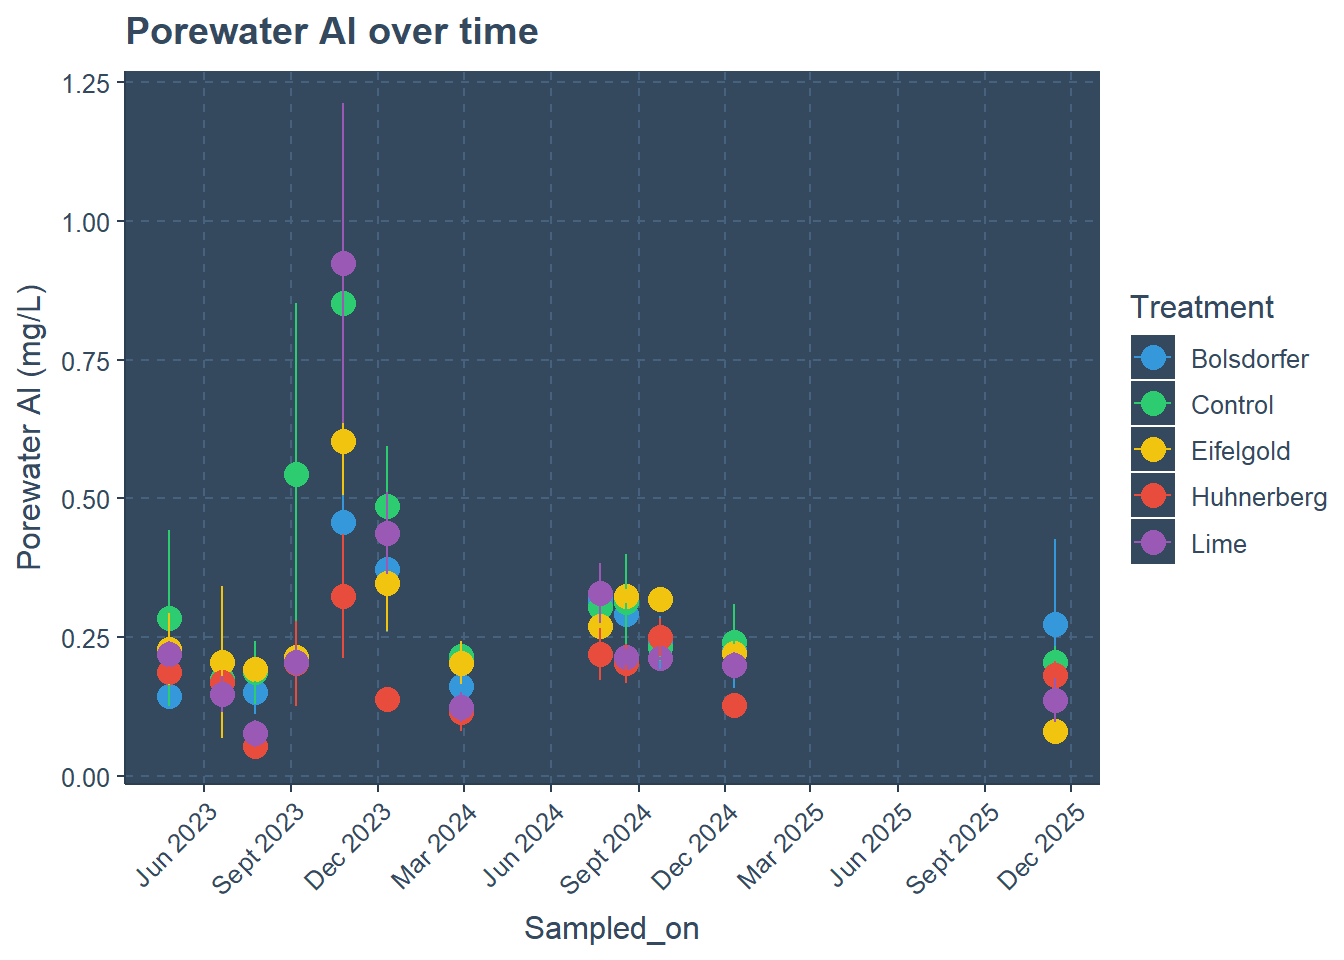
\includegraphics[width=1.0\textwidth]{figures/temporal_porewater_Al.png} 
    \caption{Temporal dynamics of soil porewater dissolved aluminium concentrations (2023--2025) across silicate, lime, and unamended control treatments at the Westmalle field trial.}
    \label{fig:temporal_porewater_Al}
\end{figure}

\newpage

\begin{figure}[htbp]
    \centering
    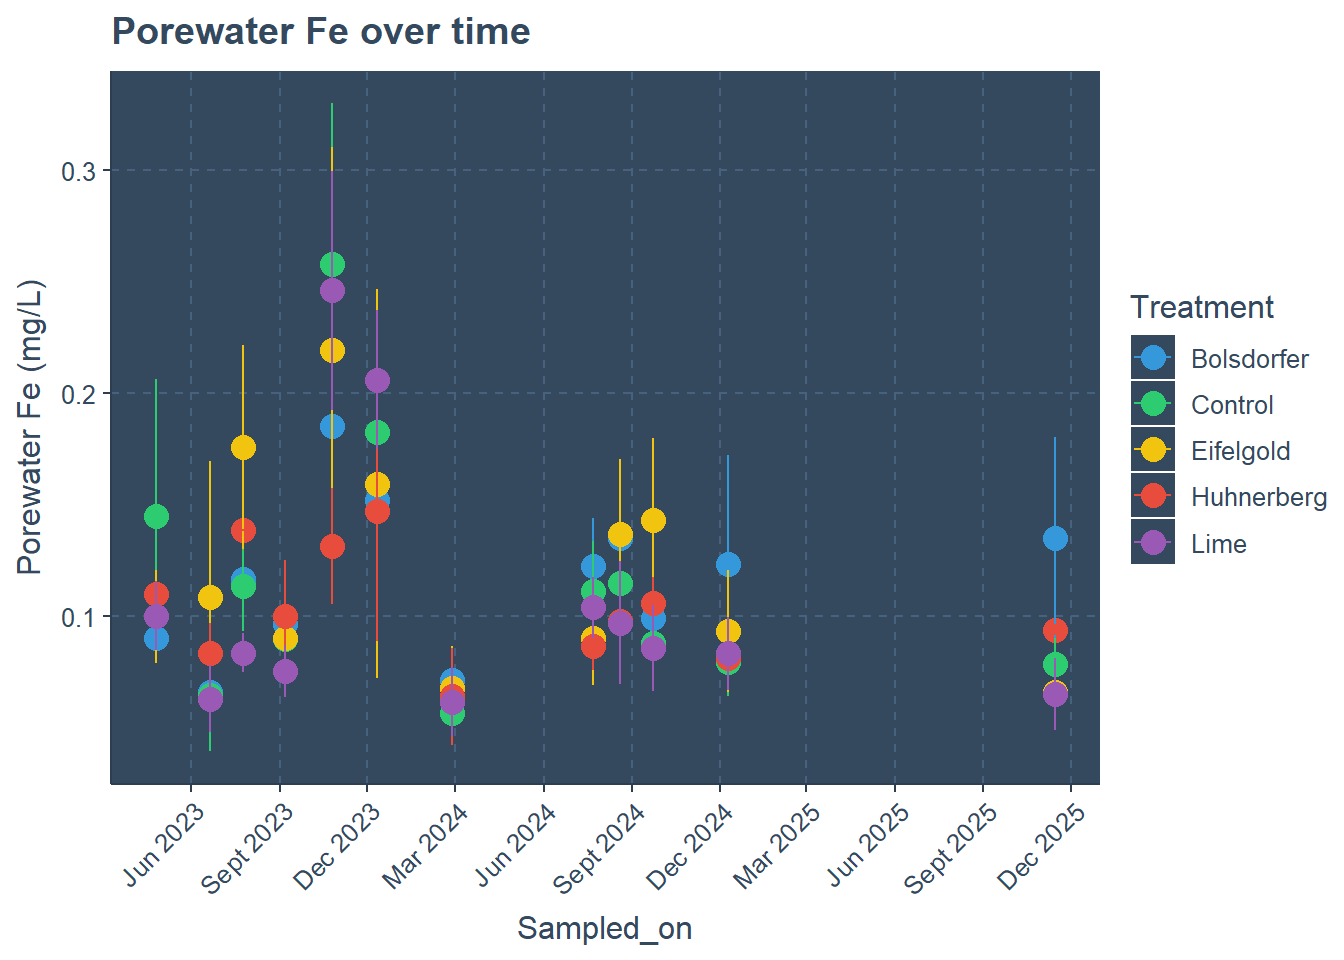
\includegraphics[width=1.0\textwidth]{figures/temporal_porewater_Fe.png} 
    \caption{Temporal dynamics of soil porewater dissolved iron concentrations (2023--2025) across silicate, lime, and unamended control treatments at the Westmalle field trial.}
    \label{fig:temporal_porewater_Fe}
\end{figure}

\newpage

\begin{figure}[htbp]
    \centering
    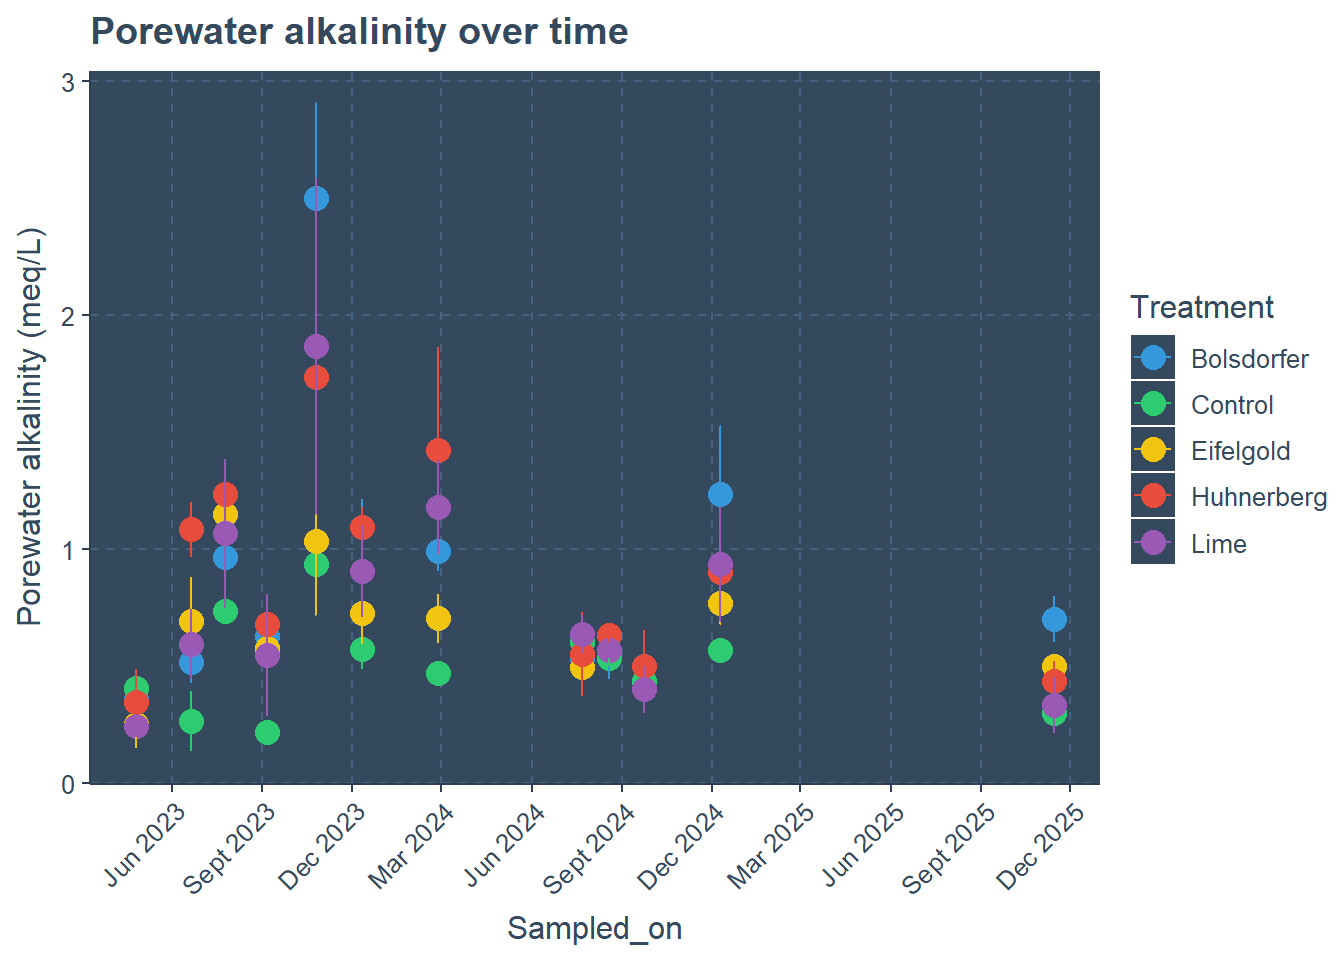
\includegraphics[width=1.0\textwidth]{figures/temporal_porewater_alkalinity.png} 
    \caption{Temporal dynamics of soil porewater carbonate alkalinity (2023-2025) across silicate, lime, and unamended control treatments at the Westmalle field trial.}
    \label{fig:temporal_porewater_alkalinity}
\end{figure}

\newpage
  
\begin{figure}[htbp]
    \centering
    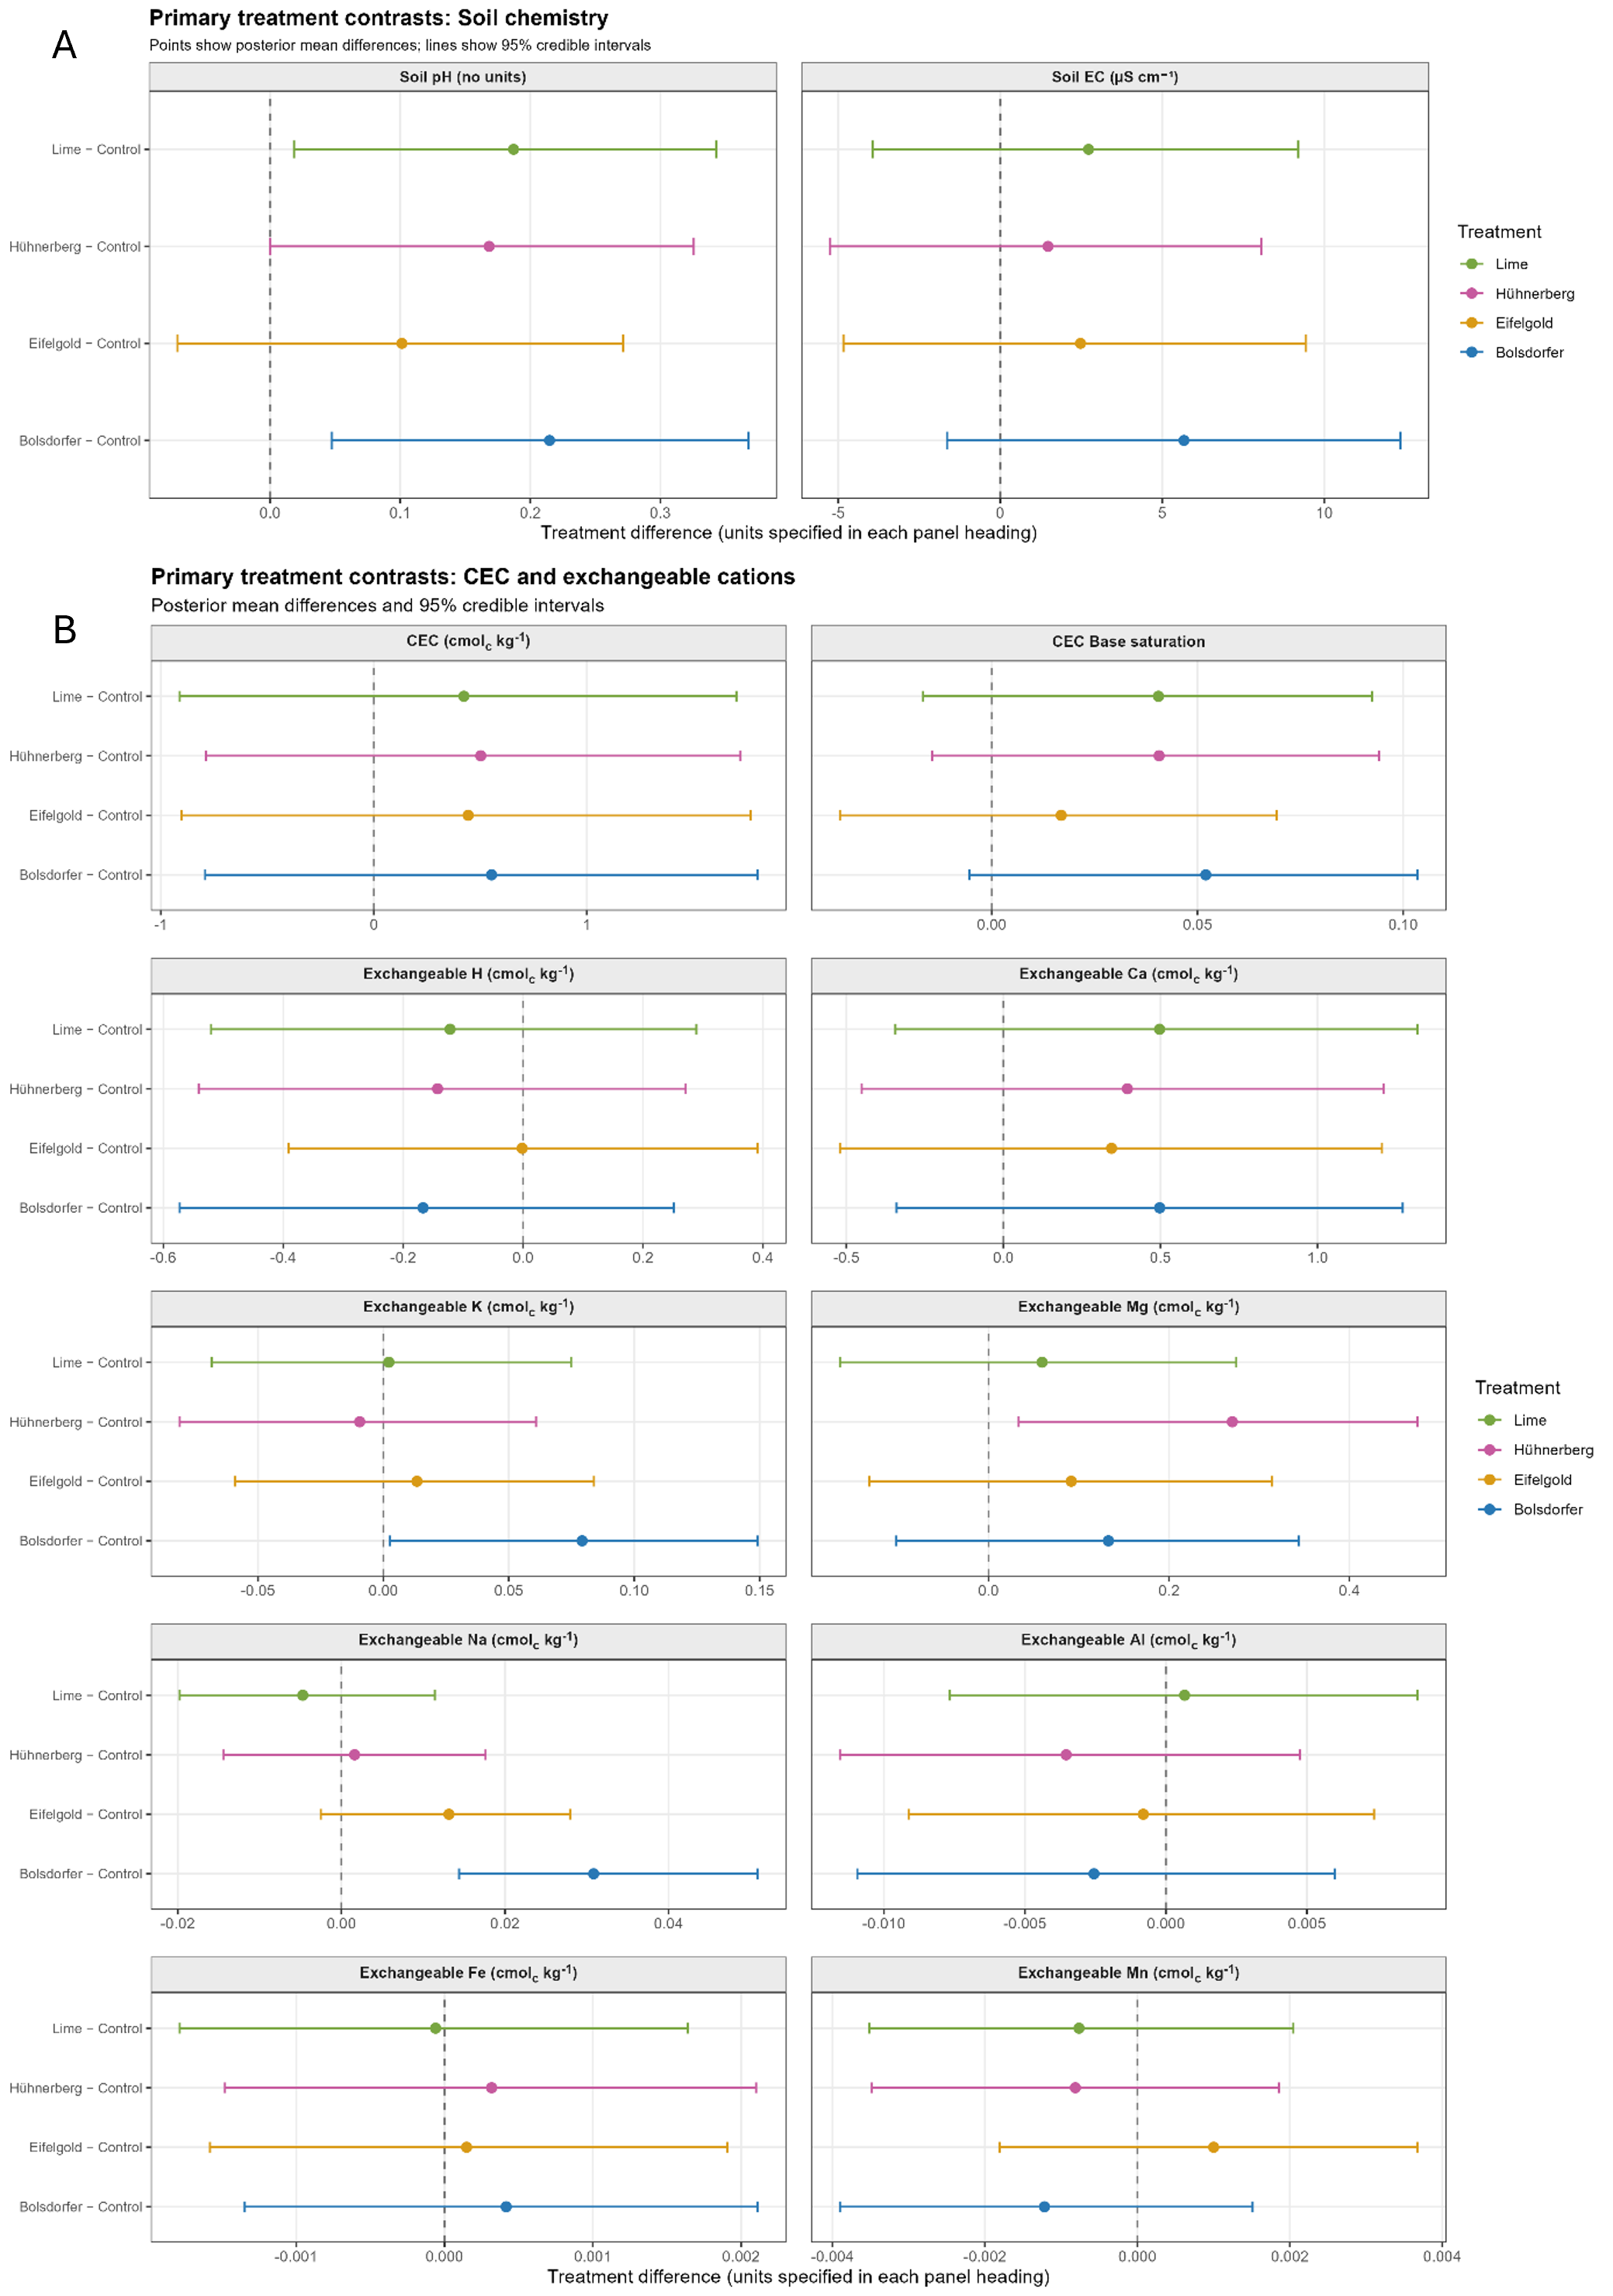
\includegraphics[width=1.0\textwidth]{figures/pHECCEC_comparison.png} 
    \caption{Bayesian treatment-versus-control comparisons for soil pH, electrical conductivity (EC), cation exchange capacity (CEC), titratable acidity, base saturation, and $\text{NH}_4\text{OAc}$-extractable exchangeable cations ($\text{Ca}, \text{Mg}, \text{K}, \text{Na}, \text{Mn}, \text{Al}, \text{Fe}$) three years after amendment application (February 2026).}
    \label{fig:pHECCEC_comparison}
\end{figure}

\newpage

\begin{figure}[htbp]
    \centering
    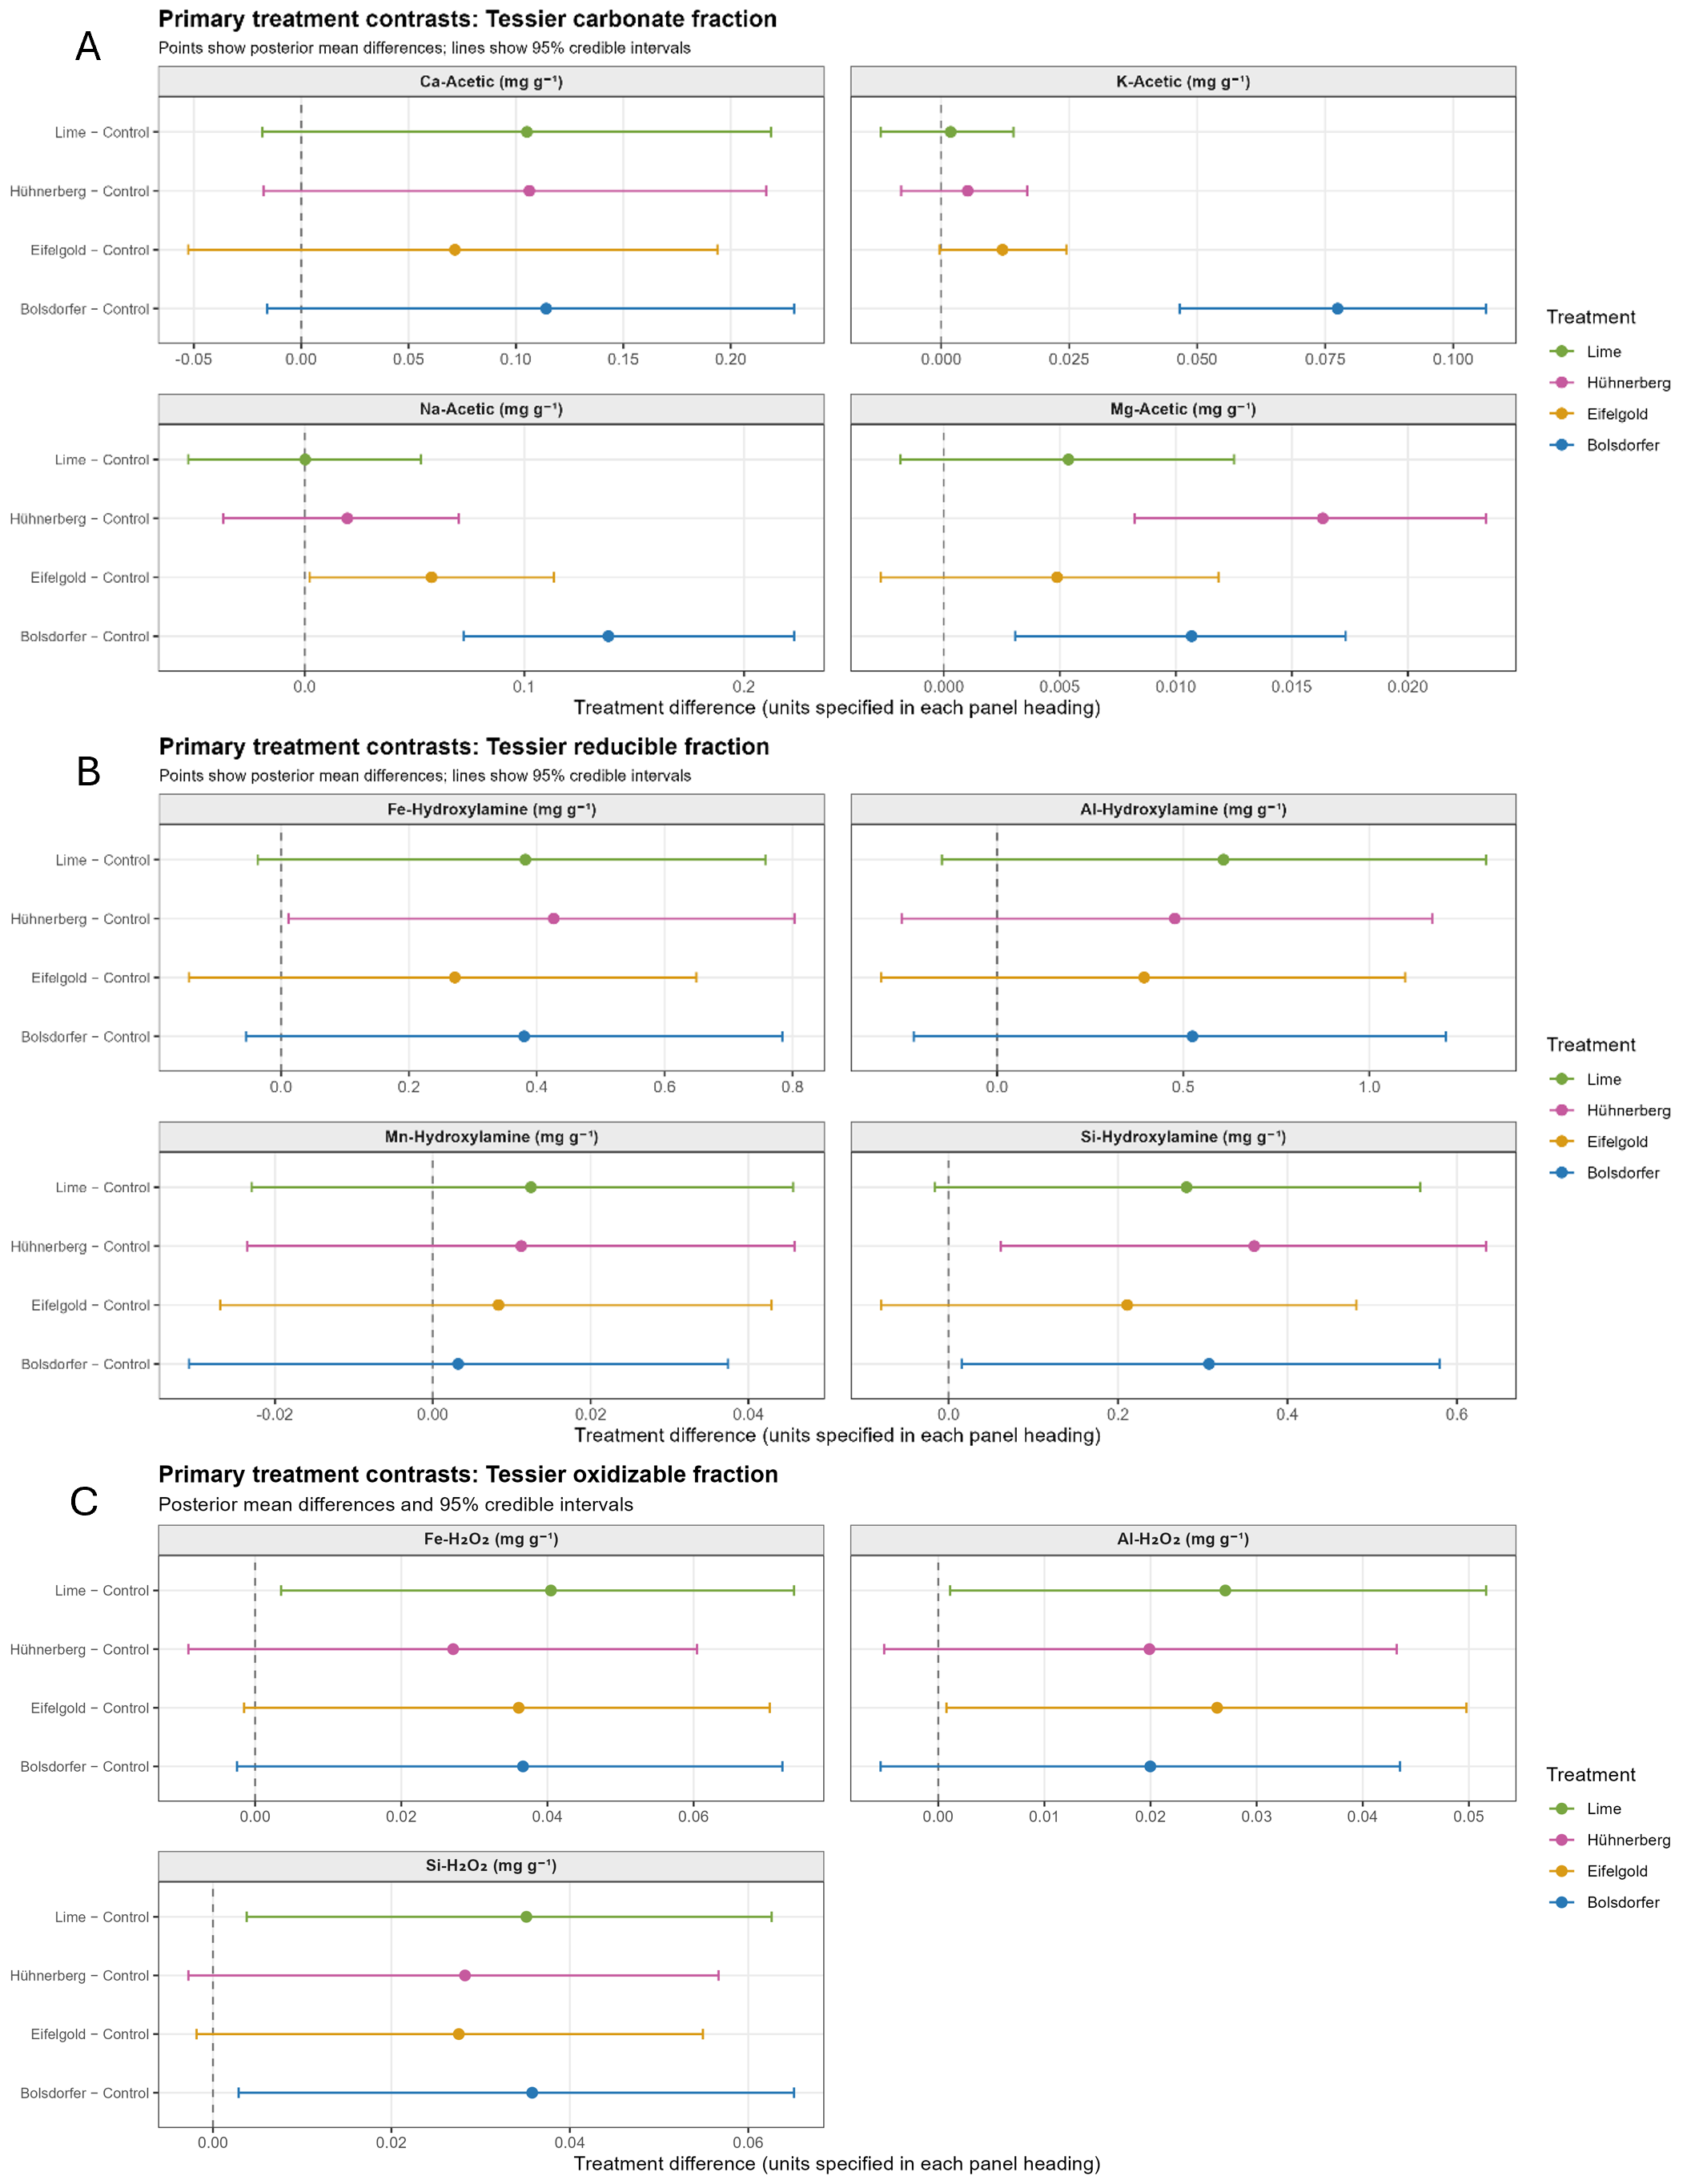
\includegraphics[width=1.0\textwidth]{figures/tessier_comparisons.png} 
    \caption{Bayesian treatment-versus-control comparisons for elements sequentially extracted via the modified Tessier procedure: 1 M acetic acid (exchangeable/carbonate-associated), hydroxylamine (reducible $\text{Fe/Mn}$ oxide-associated), and $\text{H}_2\text{O}_2$ (oxidizable/organic-matter-associated) fractions.}
\end{figure}

\newpage

\begin{figure}[htbp]
    \centering
    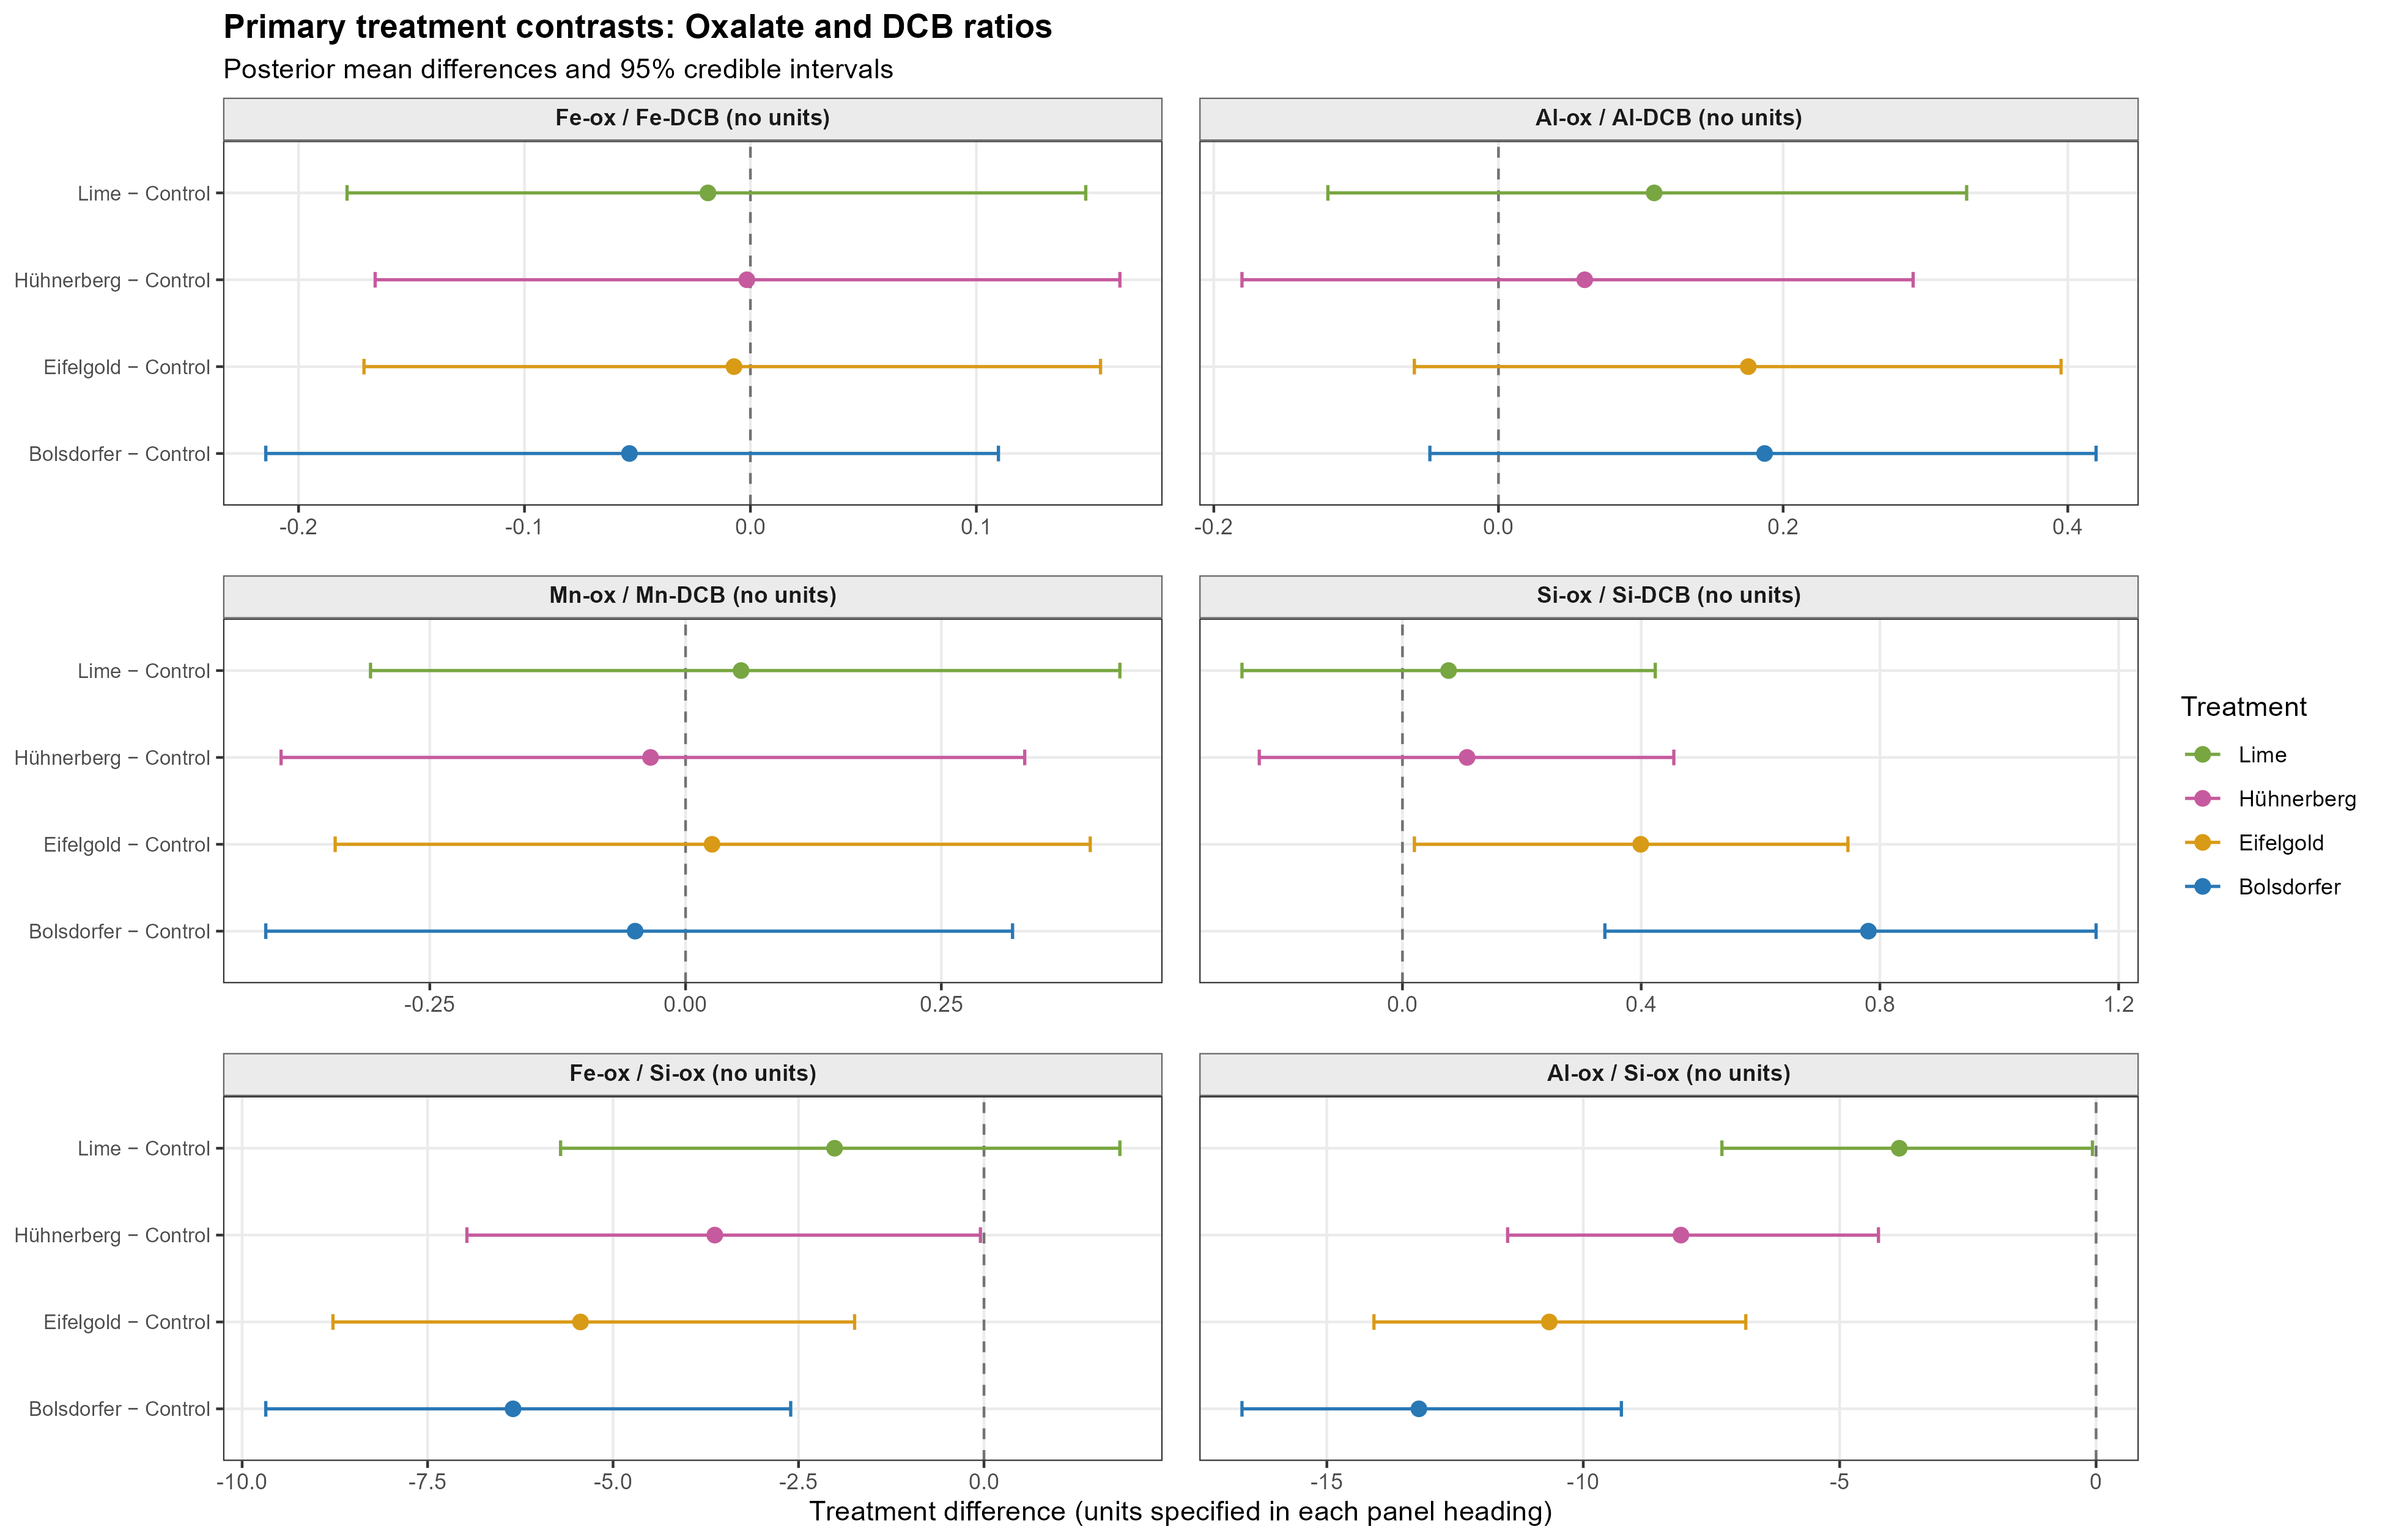
\includegraphics[width=1.0\textwidth]{figures/Oxalate_DCB_comparisons.png} 
    \caption{Bayesian treatment-versus-control comparisons for ratios of poorly crystalline/short-range-order oxide-associated elements (0.2 M acid ammonium oxalate, pH 3, dark) relative to crystalline plus poorly crystalline oxides (dithionite-citrate-bicarbonate, DCB) and elemental $\text{Fe:Si}$ and $\text{Al:Si}$ oxalate ratios.}
    \label{fig:Oxalate_DCB_comparisons}
\end{figure}

\newpage

\begin{figure}[htbp]
    \centering
    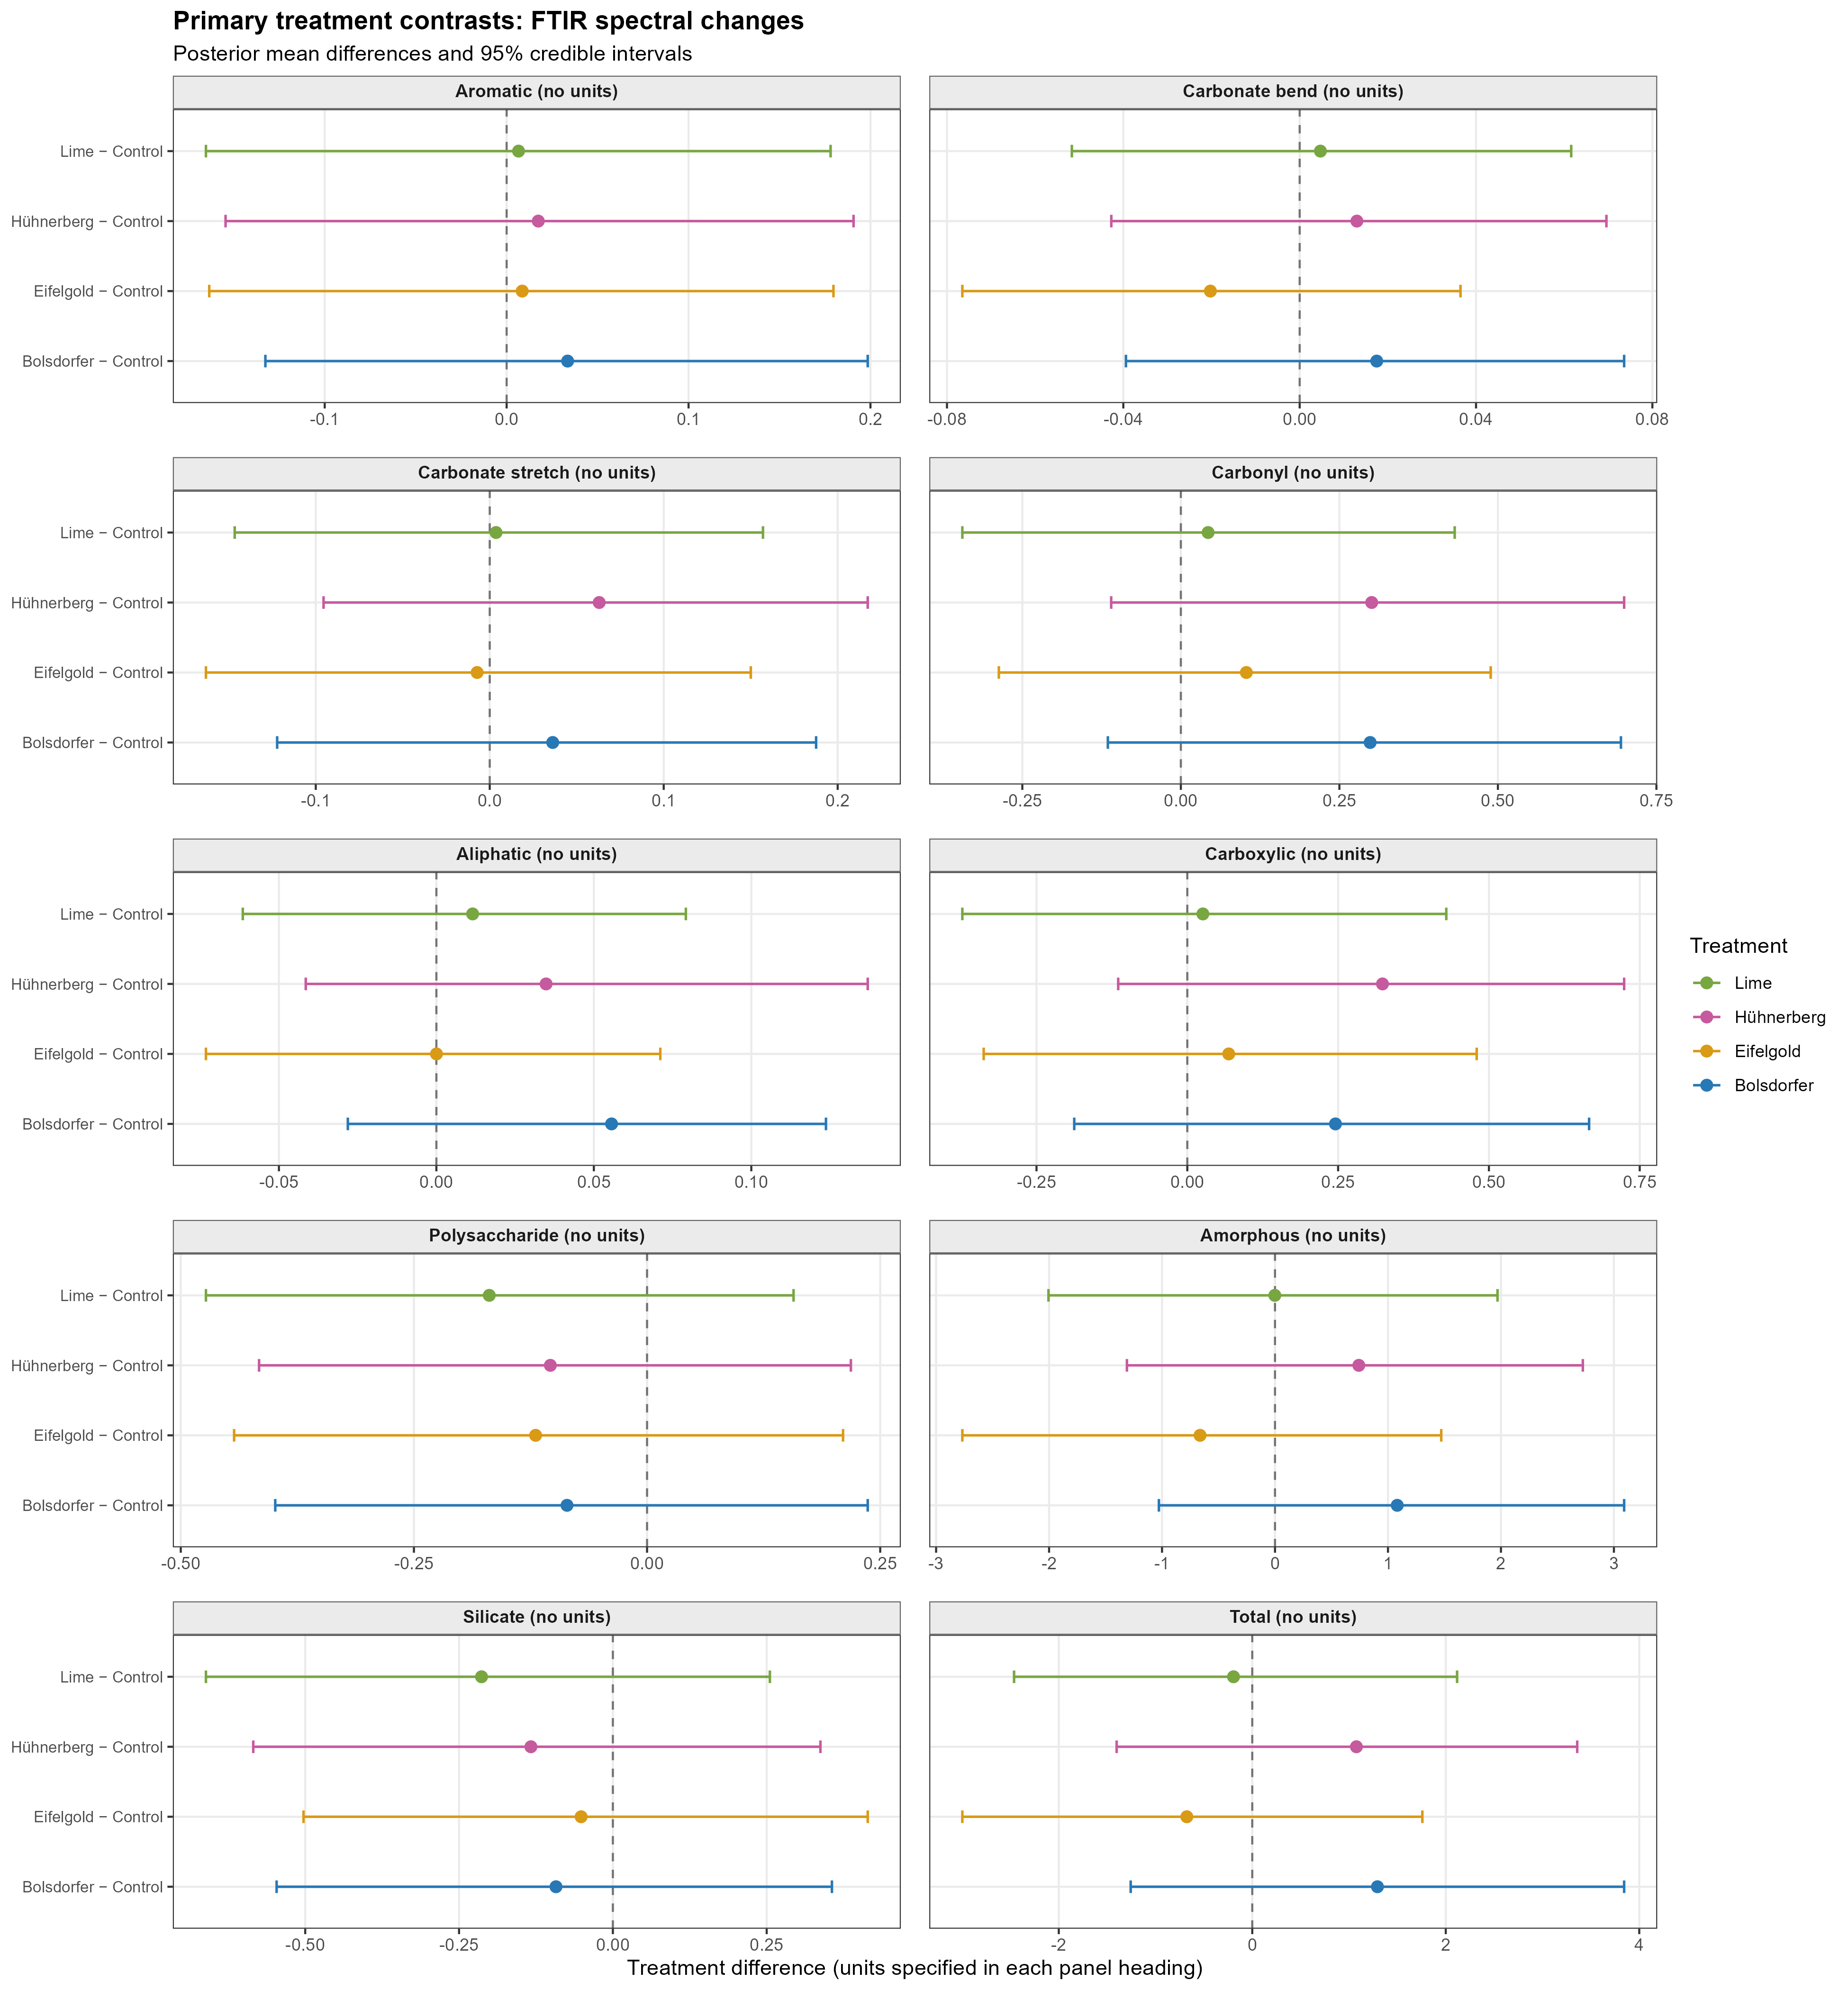
\includegraphics[width=1.0\textwidth]{figures/FTIR_comparison.png} 
    \caption{Bayesian treatment-versus-control comparisons of relative changes ($\Delta A_{\text{band}}$, \%) in integrated ATR-FTIR band areas following 1 M $\text{NH}_4\text{OAc}$ (pH 7) cation extraction on ALS baseline-corrected, L2 vector-normalised spectra (800--3000 cm$^{-1}$). 
    \label{fig:FTIR_comparison}
\end{figure}


\newpage

\begin{figure}[htbp]
    \centering
    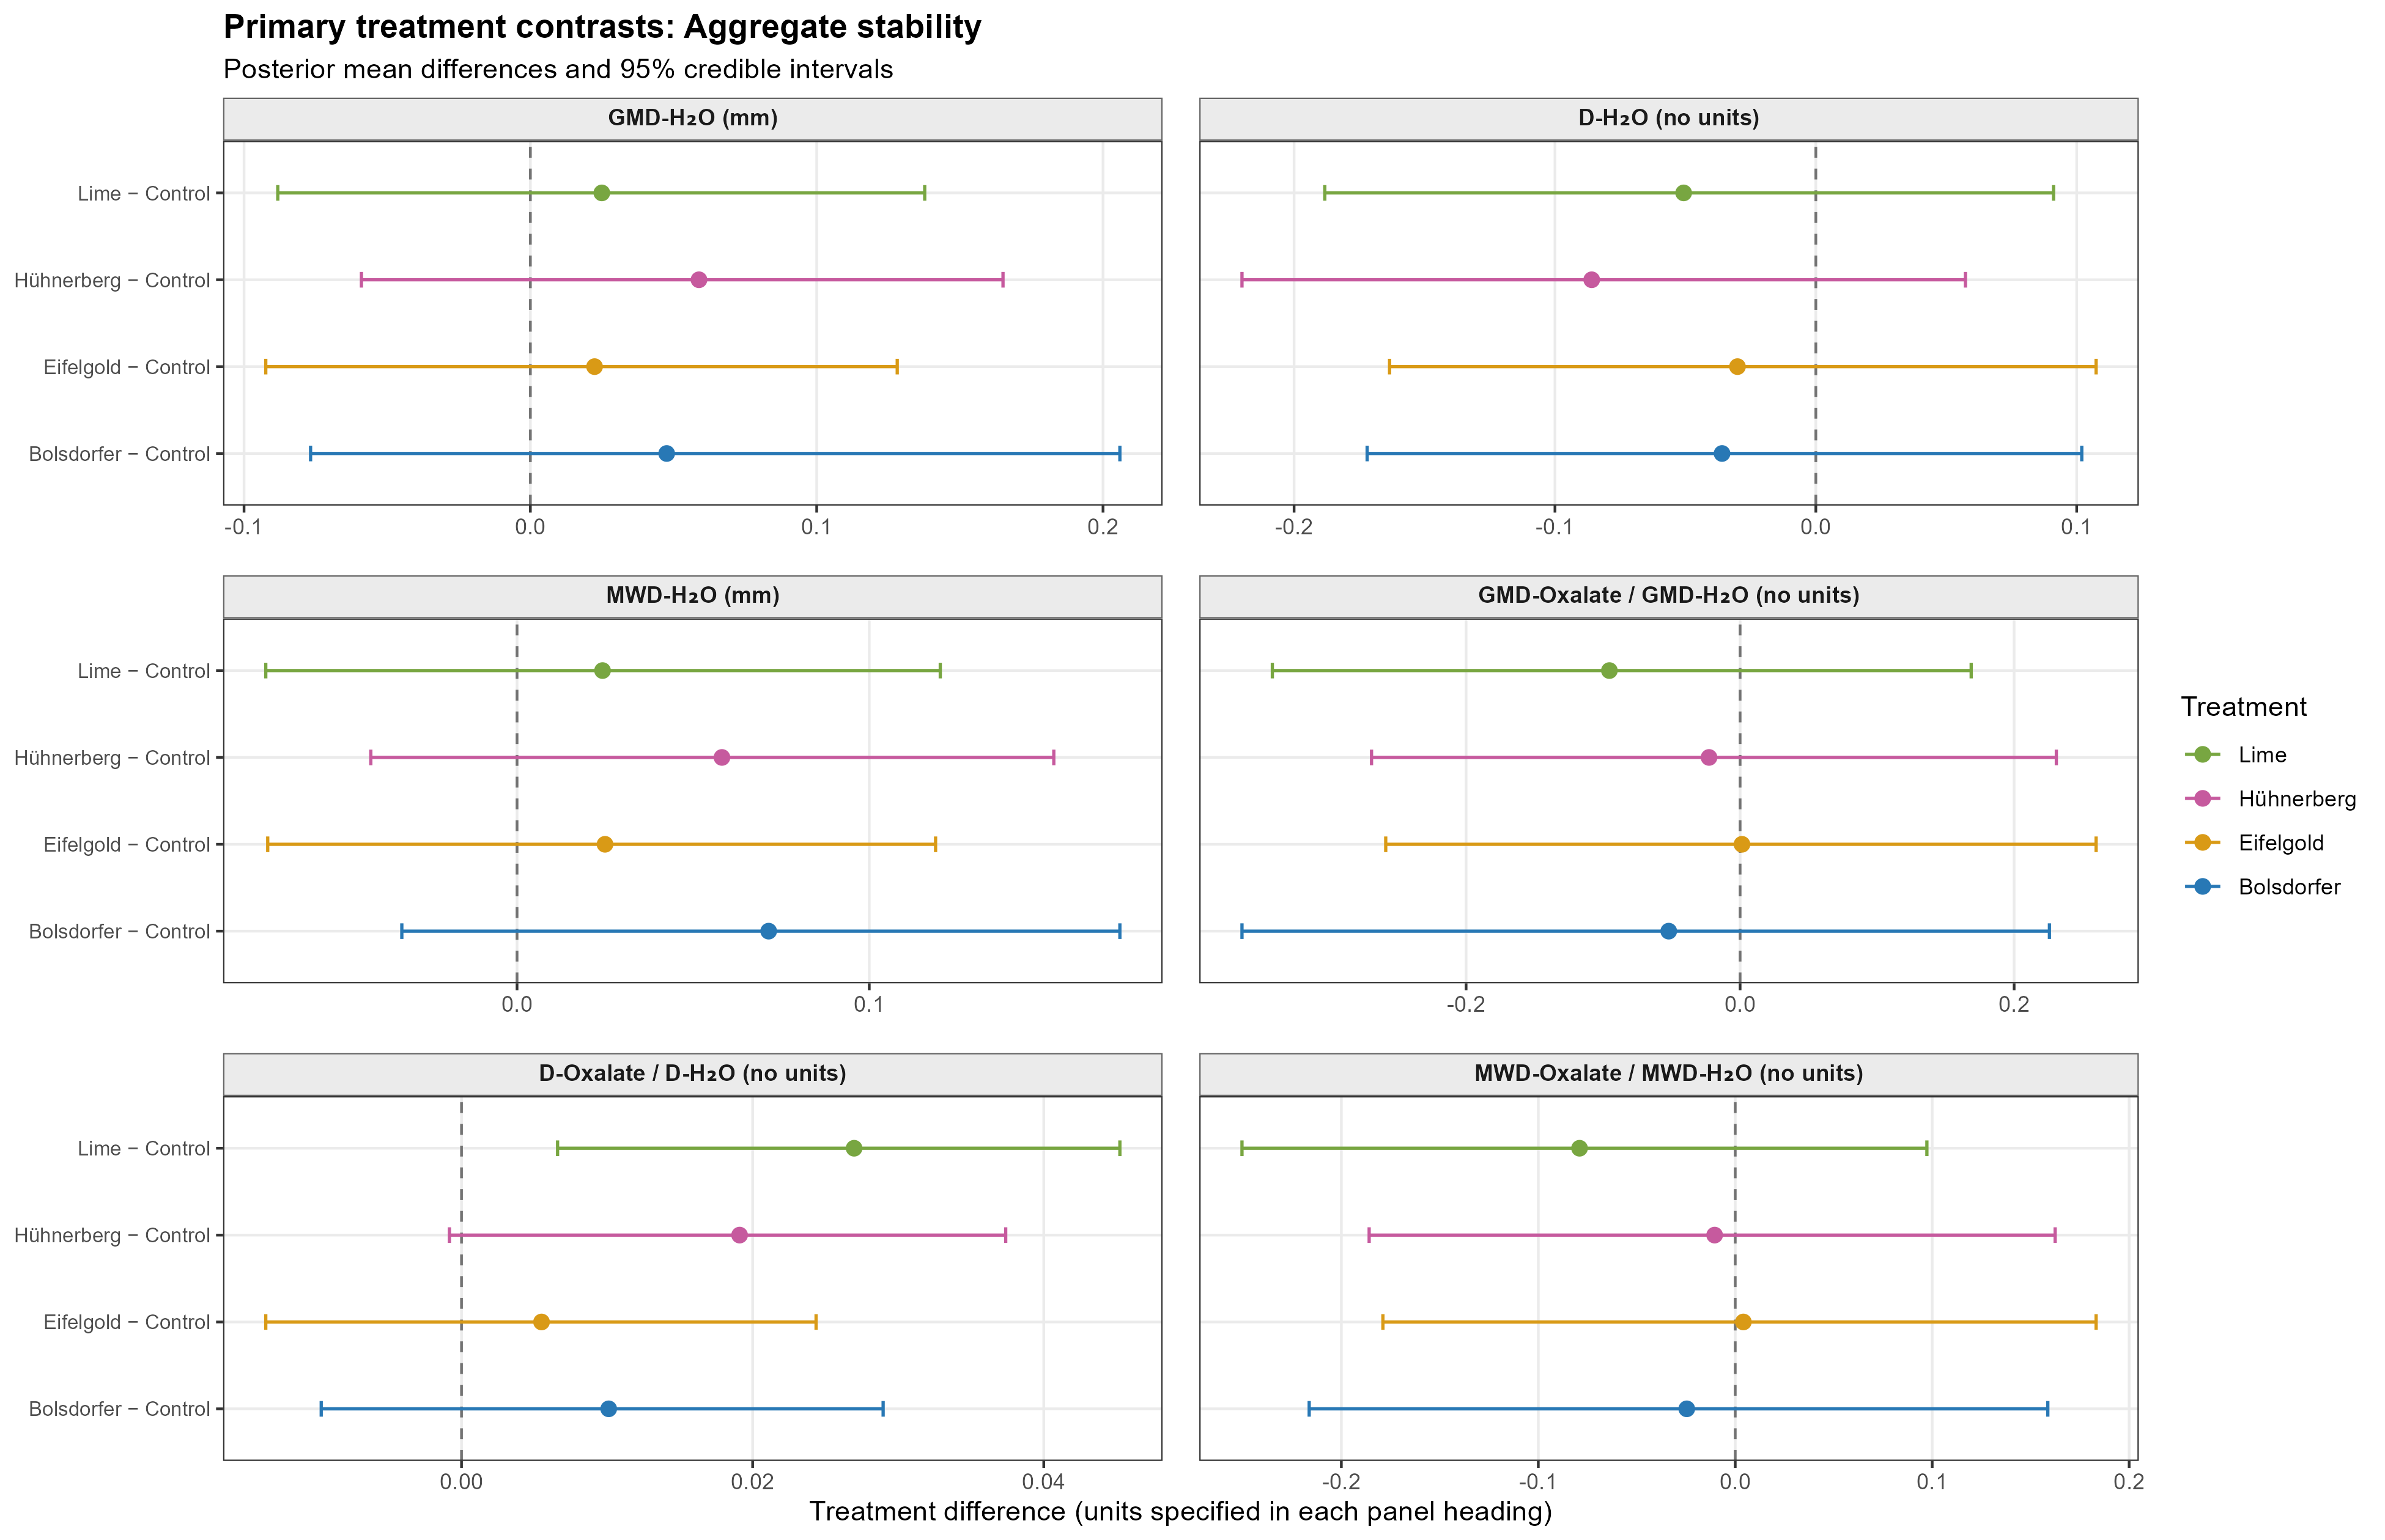
\includegraphics[width=1.0\textwidth]{figures/aggstab_comparison.png} 
    \caption{Bayesian treatment-versus-control comparisons for wet-sieving aggregate stability indices—mean weight diameter (MWD), geometric mean diameter (GMD), and fractal dimension ($D$)—under baseline $\text{H}_2\text{O}$ soaking and as $\text{Oxalate}:\text{H}_2\text{O}$ ratios isolating oxalate-extractable cementing phases.}
    \label{fig:aggstab_comparison}
\end{figure}

\newpage

\begin{figure}[htbp]
    \centering
    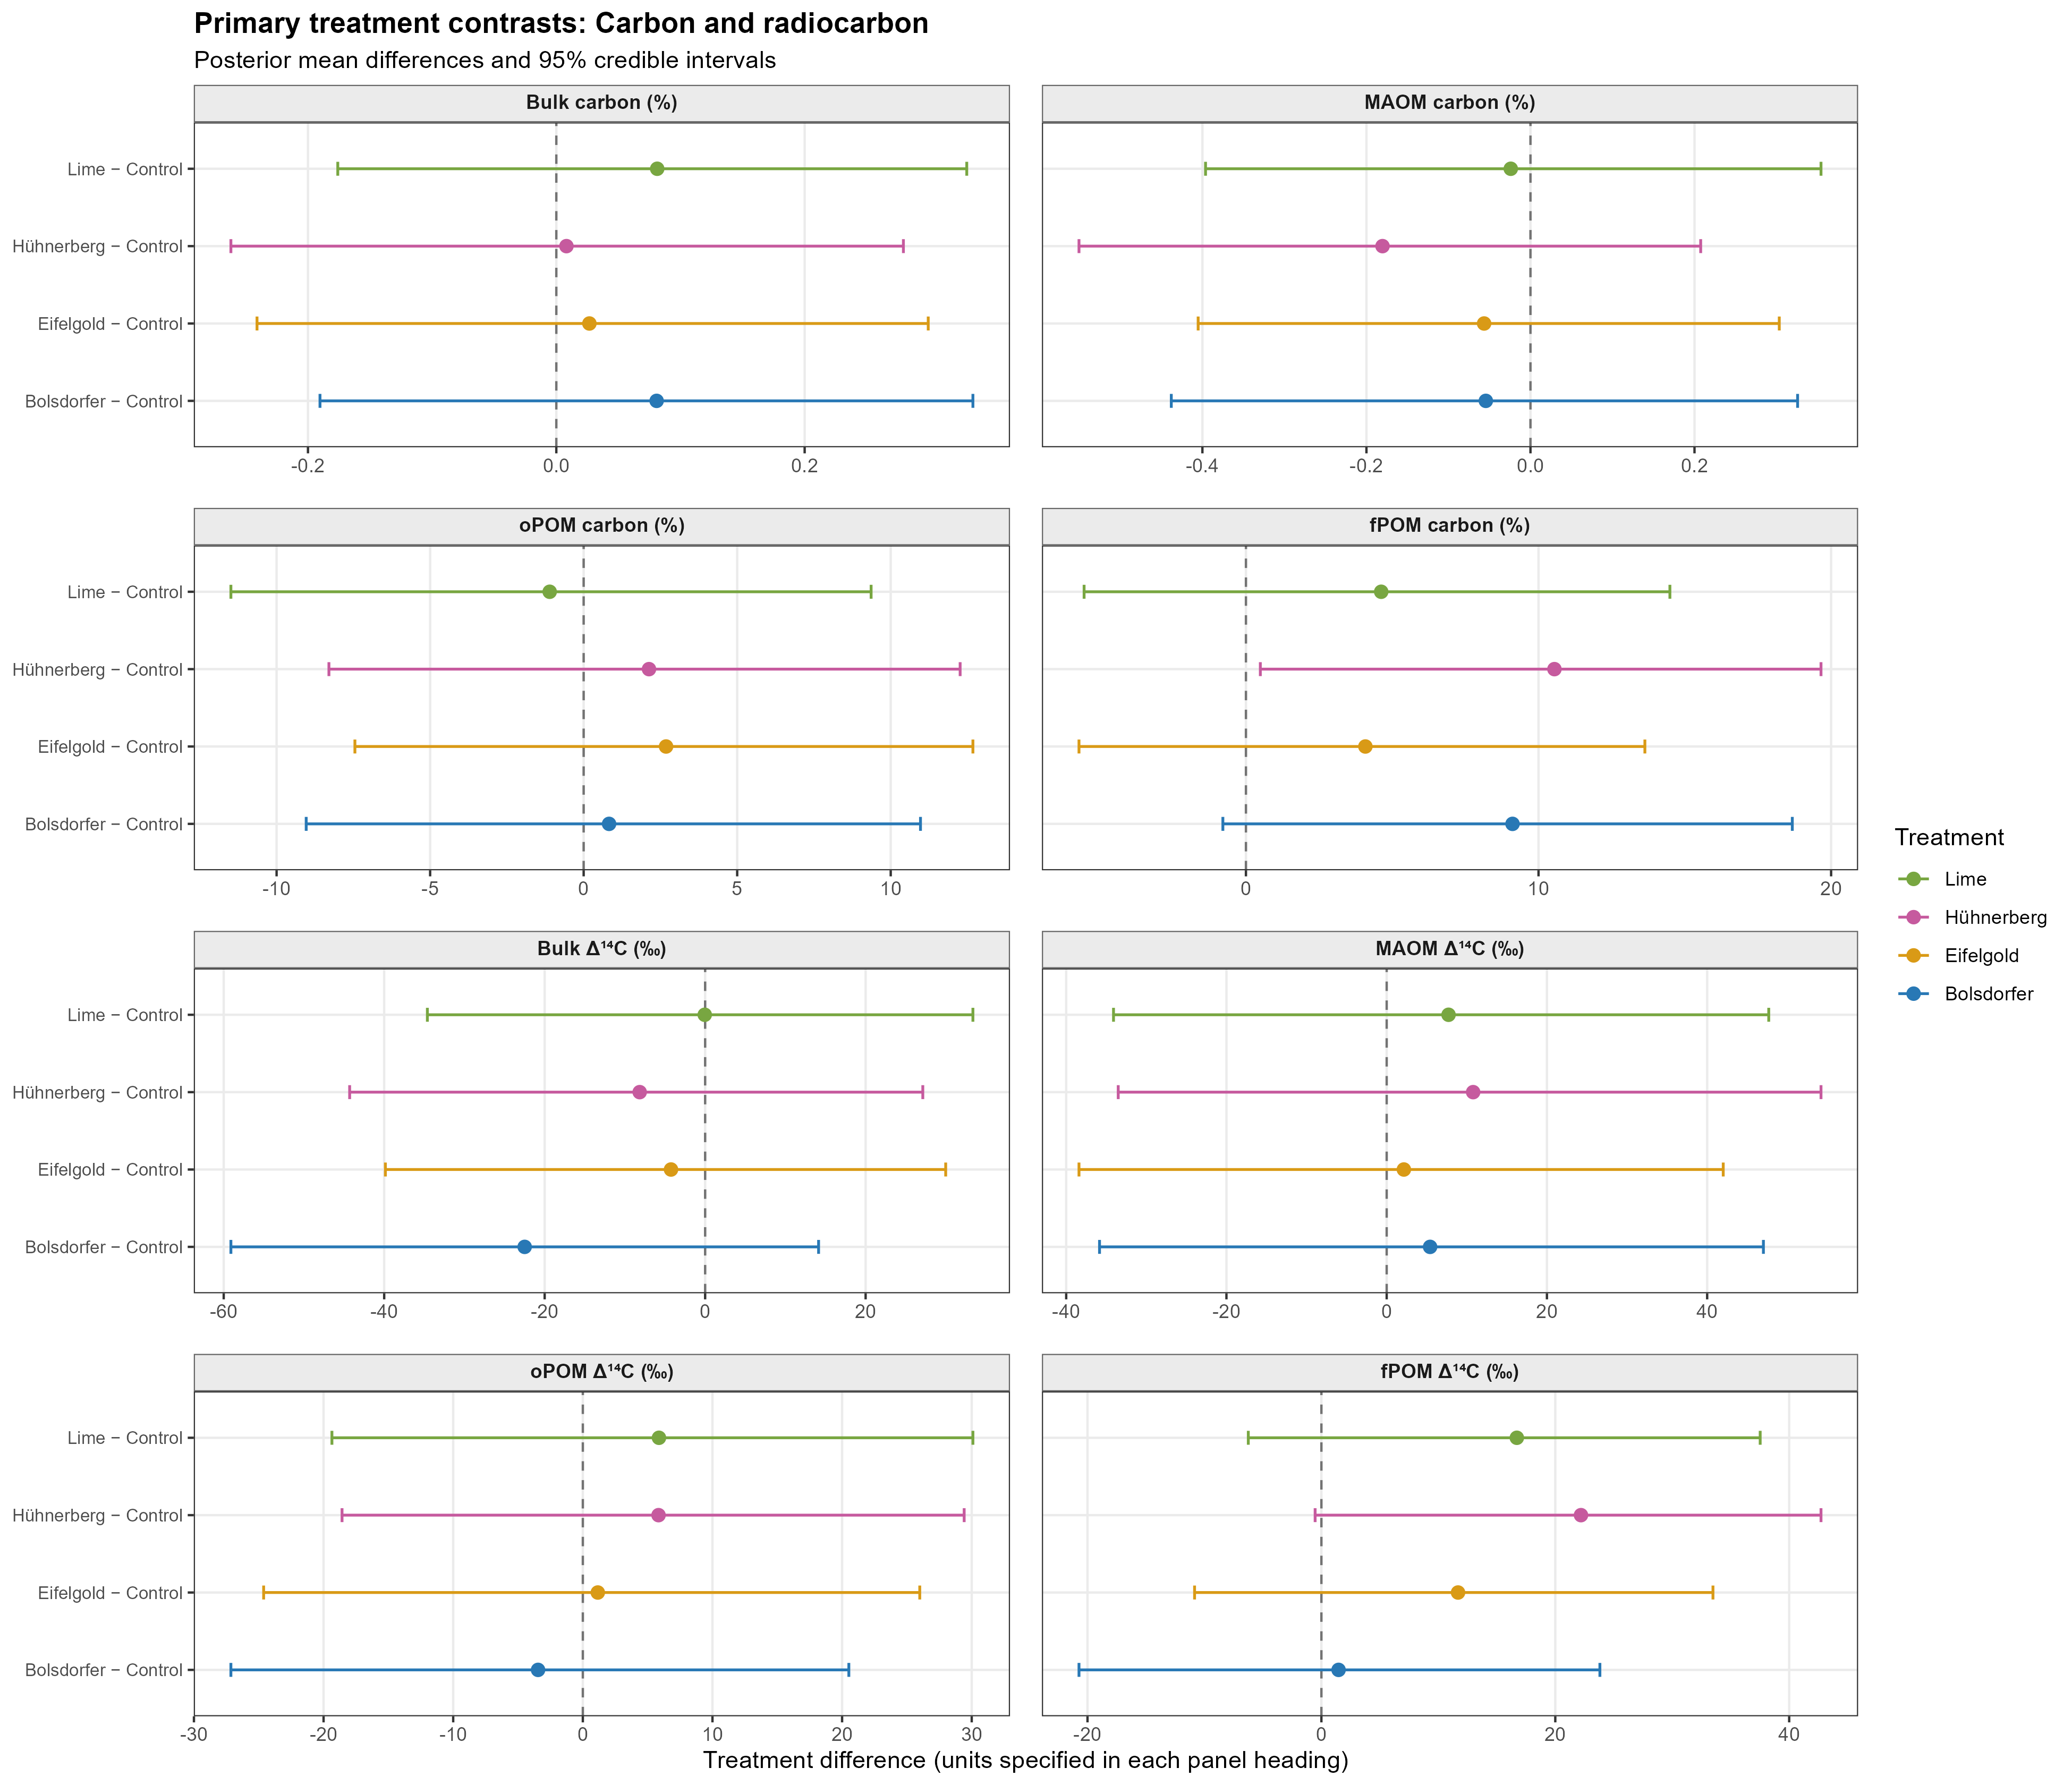
\includegraphics[width=1.0\textwidth]{figures/C14C_comparison.png} 
    \caption{Bayesian treatment-versus-control comparisons of organic carbon concentrations and radiocarbon signatures ($\Delta^{14}\text{C}$, \textperthousand{}) in bulk soil and sodium polytungstate (SPT, $1.60\text{--}1.62\text{ g cm}^{-3}$) density fractions: free particulate (fPOM), occluded particulate (oPOM, dispersed at $450\text{ J mL}^{-1}$), and mineral-associated organic matter (MAOM).}
    \label{fig:C14C_comparison}
\end{figure}

\newpage

% density and pair plots SoilR modeled pars 
\begin{figure}[htbp]
    \centering
    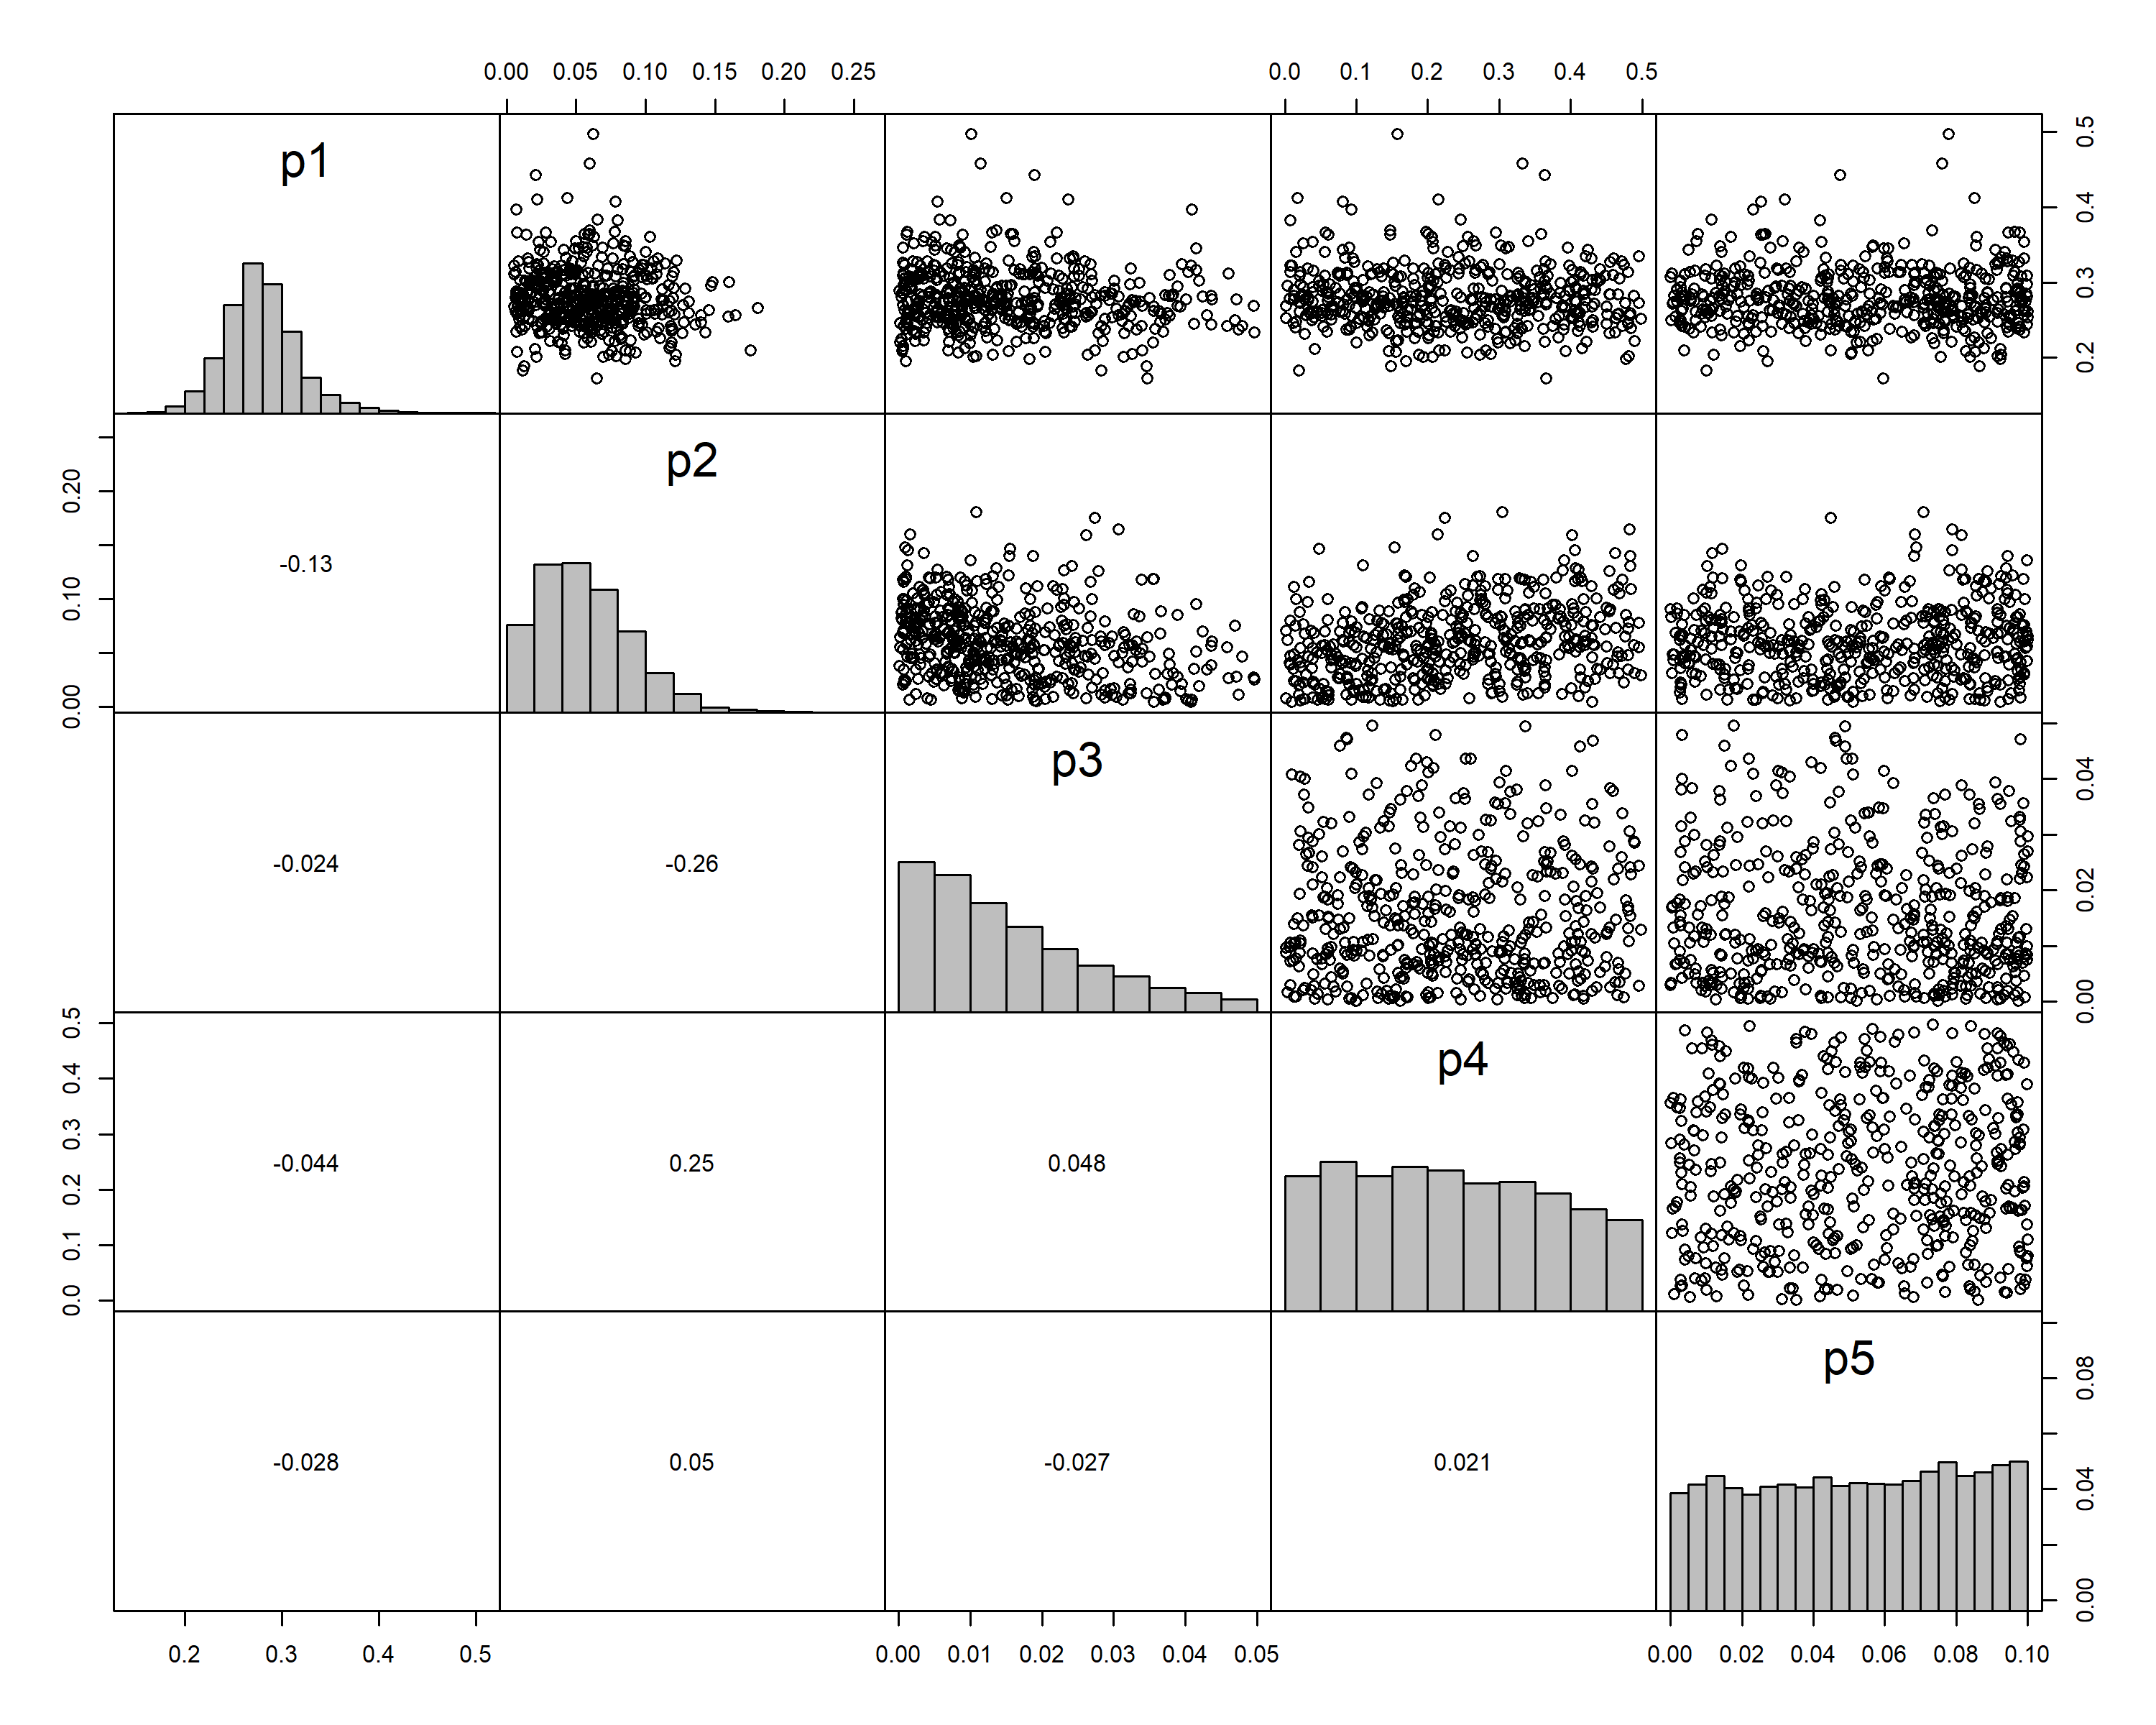
\includegraphics[width=1.0\textwidth]{figures/pairs_plot_control.png} 
    \caption{Marginal posterior density and bivariate pairs plots for SoilR three-pool compartmental parameters ($k_f, k_i, k_s$, $\alpha_{fi}, \alpha_{is}$) from adaptive Metropolis MCMC sampling in Control plots.}
    \label{fig:pairs_plot_control}
\end{figure}

\newpage

\begin{figure}[htbp]
    \centering
    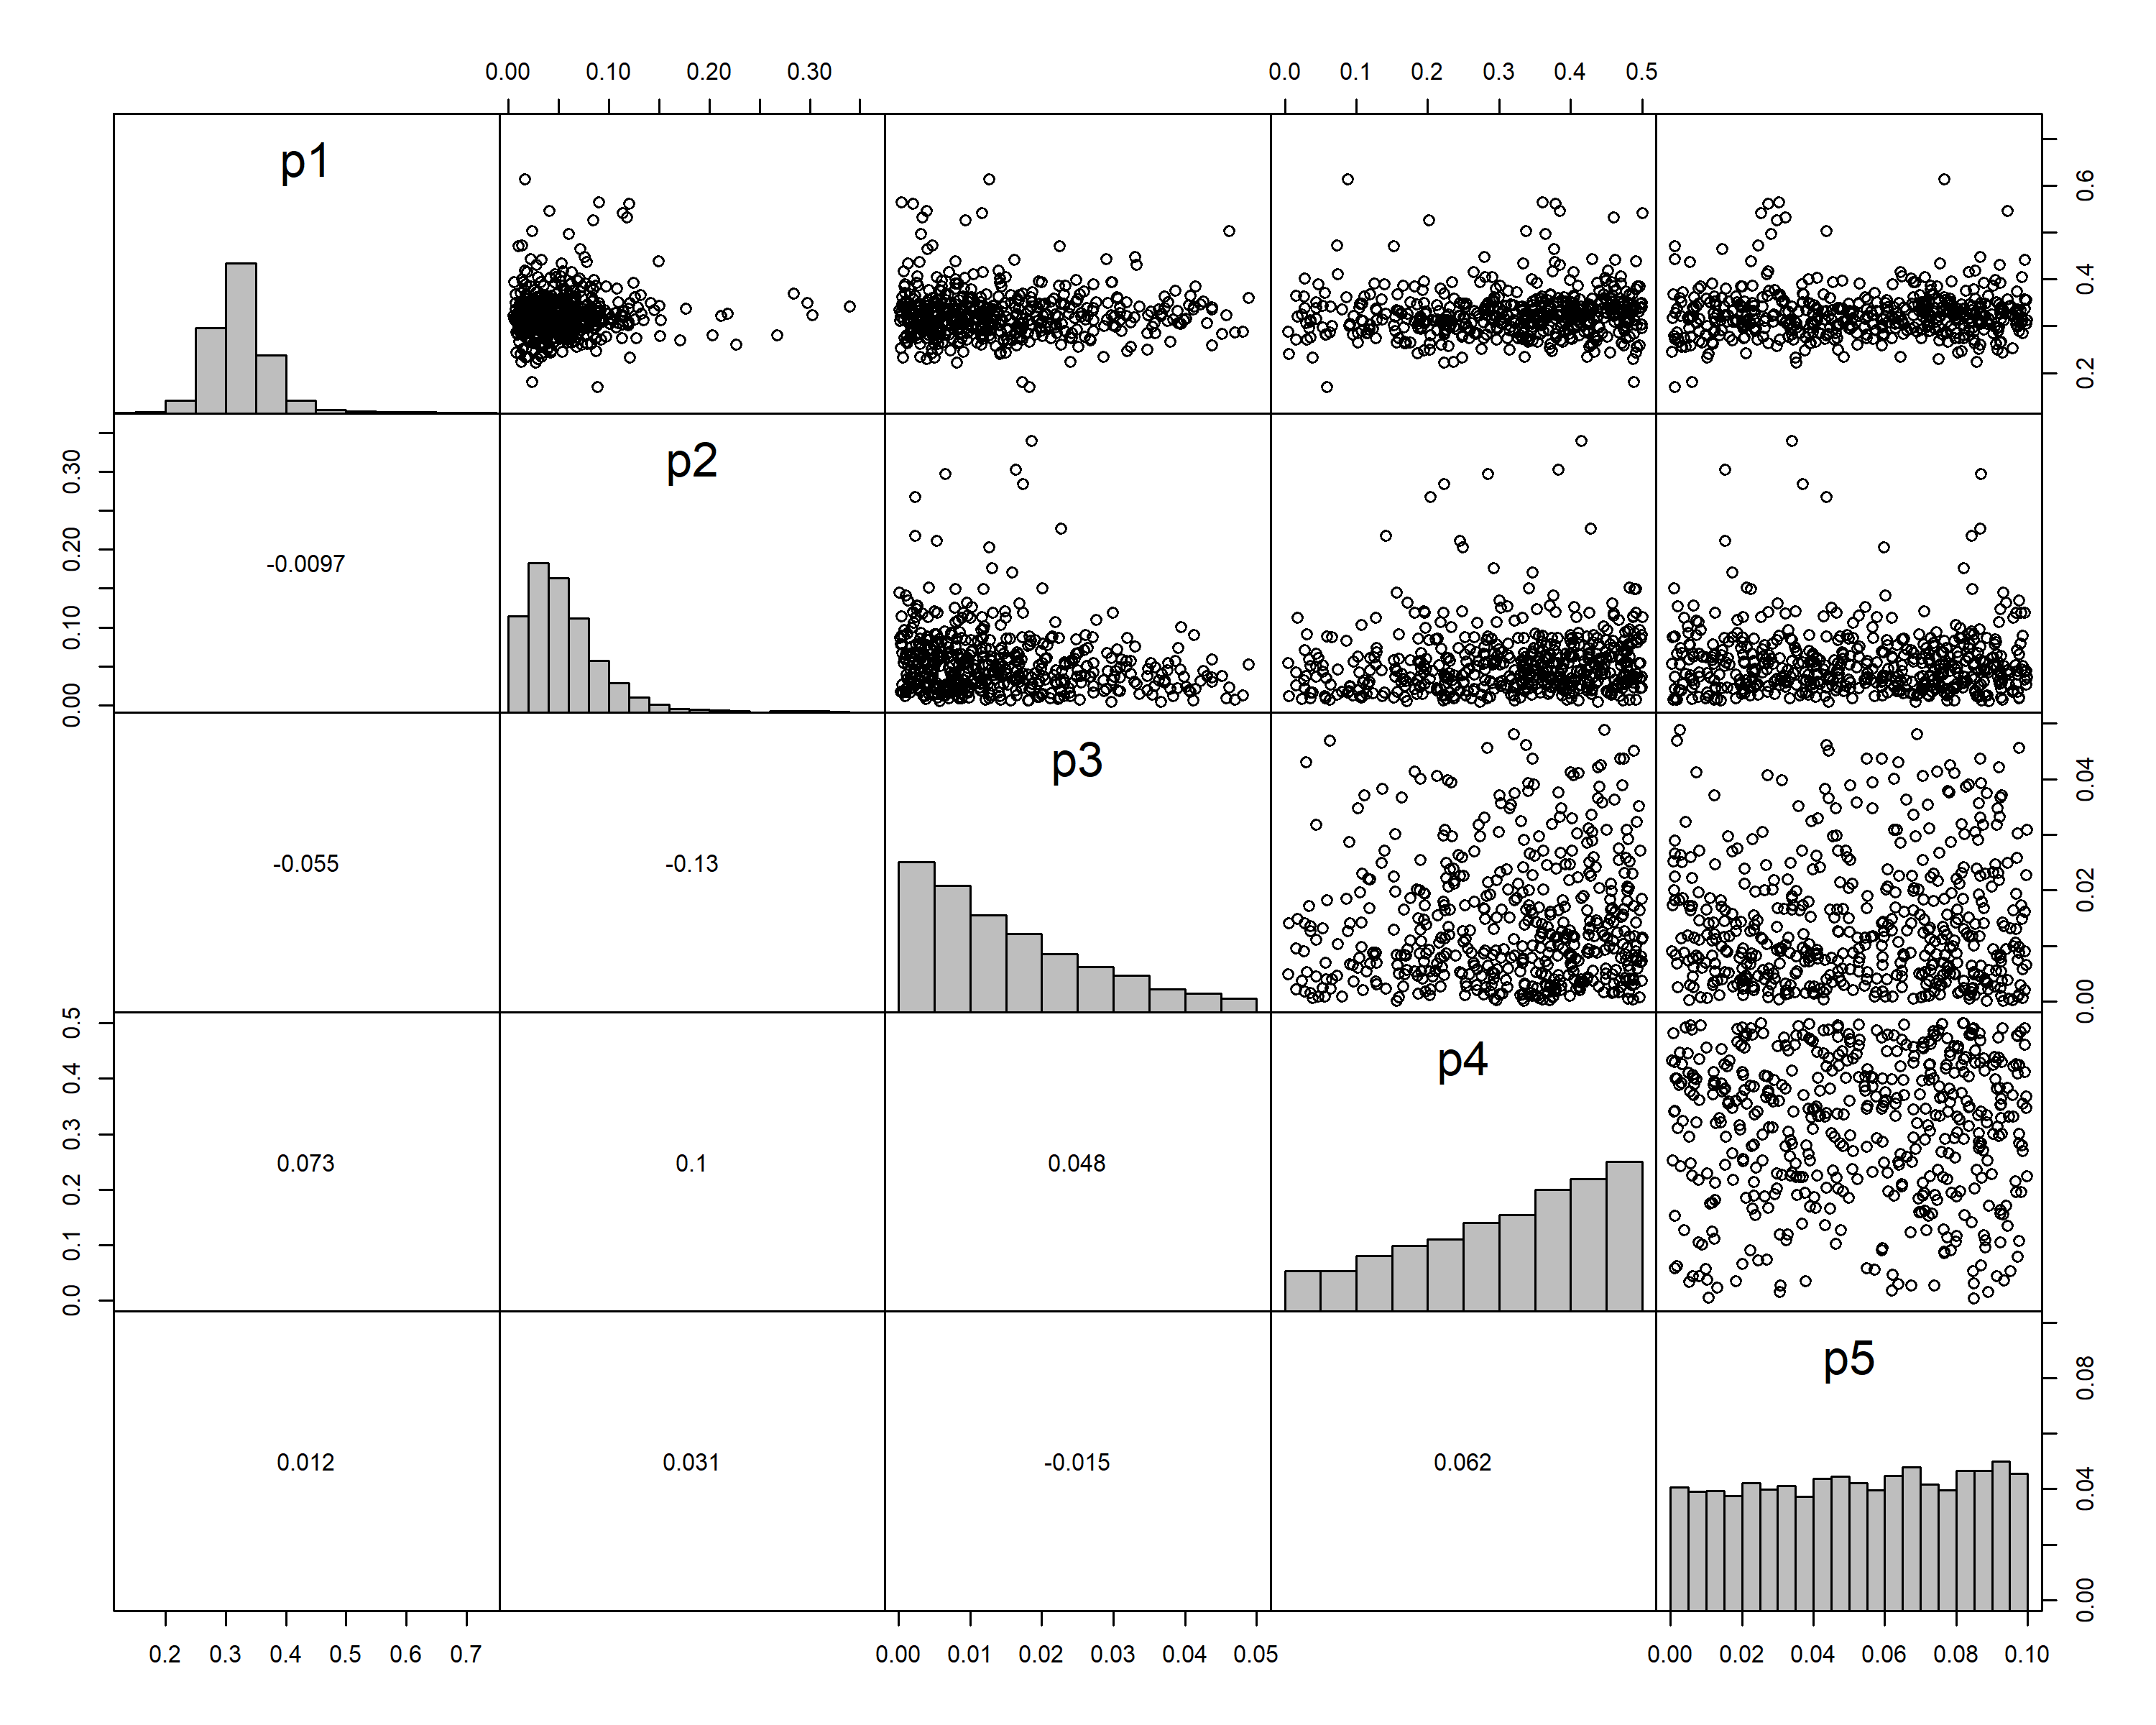
\includegraphics[width=1.0\textwidth]{figures/pairs_plot_Bolsdorfer.png} 
    \caption{Marginal posterior density and bivariate pairs plots for SoilR three-pool compartmental parameters ($k_f, k_i, k_s$, $\alpha_{fi}, \alpha_{is}$) from adaptive Metropolis MCMC sampling in Bolsdorfer basalt plots.}
    \label{fig:pairs_plot_Bolsdorfer}
\end{figure}

\newpage

\begin{figure}[htbp]
    \centering
    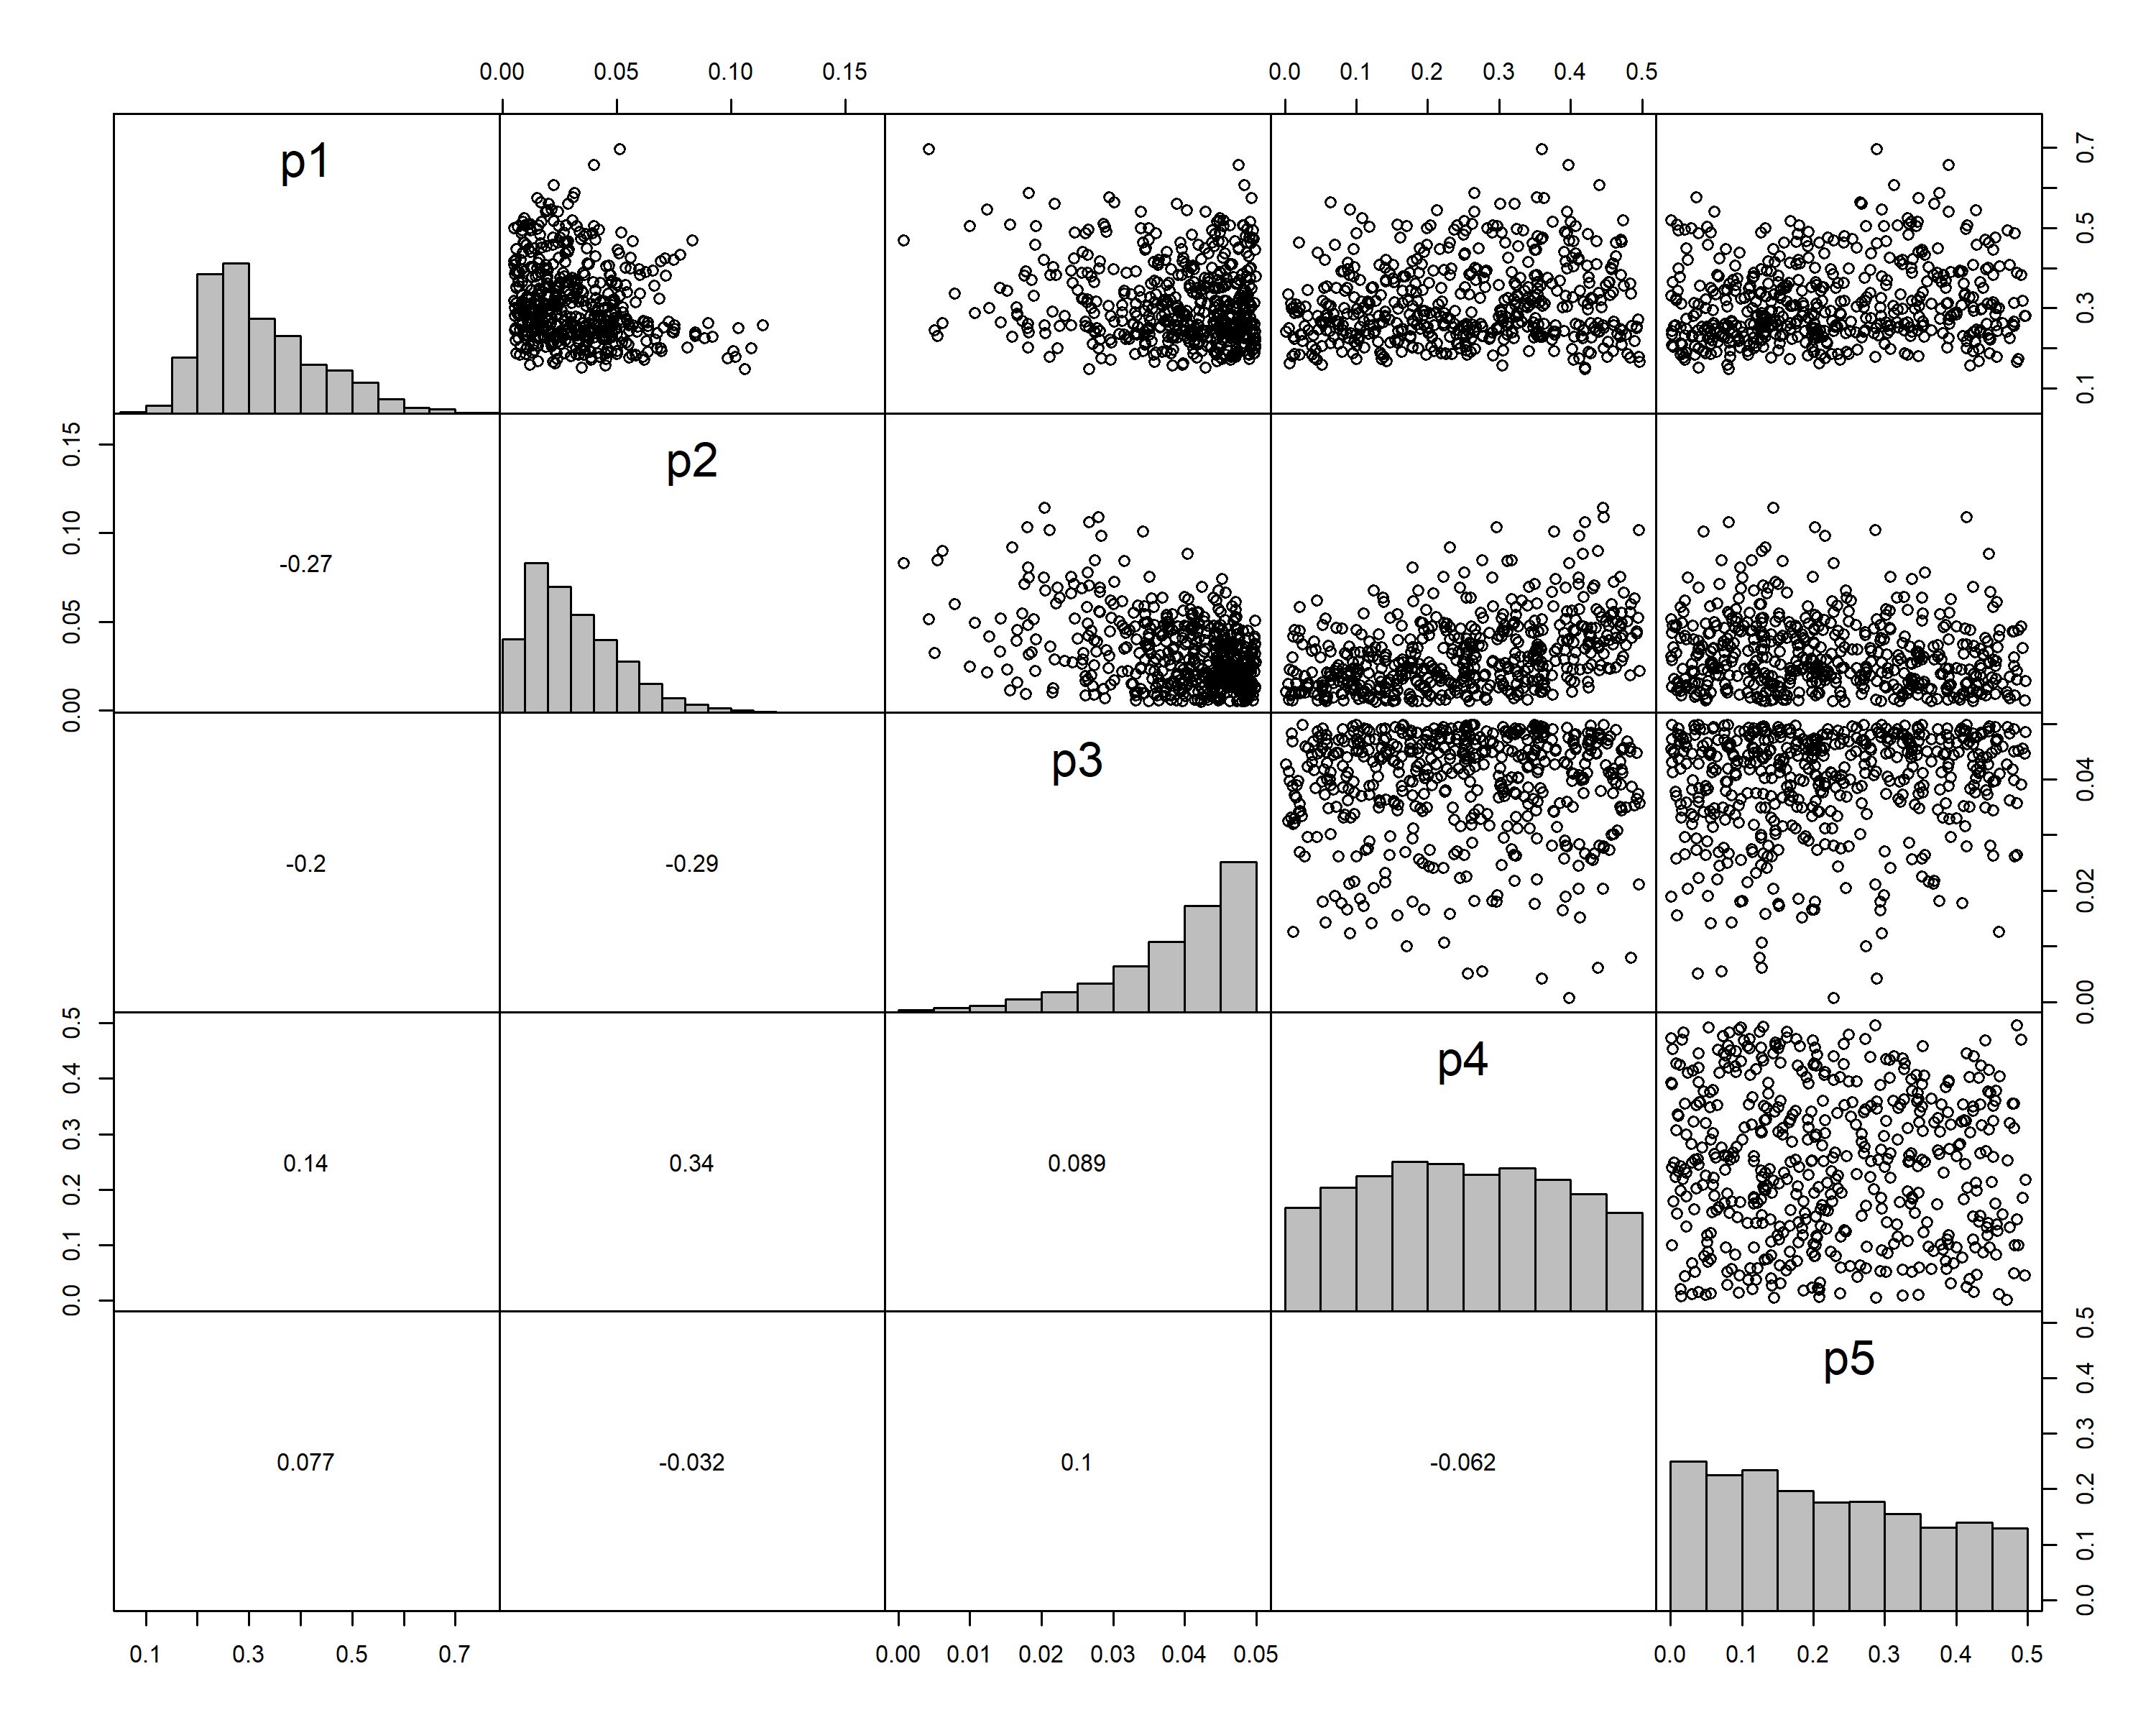
\includegraphics[width=1.0\textwidth]{figures/pairs_plot_Huhnerberg.png} 
    \caption{Marginal posterior density and bivariate pairs plots for SoilR three-pool compartmental parameters ($k_f, k_i, k_s$, $\alpha_{fi}, \alpha_{is}$) from adaptive Metropolis MCMC sampling in Hühnerberg basalt plots.}
    \label{fig:pairs_plot_Huhnerberg}
\end{figure}

\newpage

\begin{figure}[htbp]
    \centering
    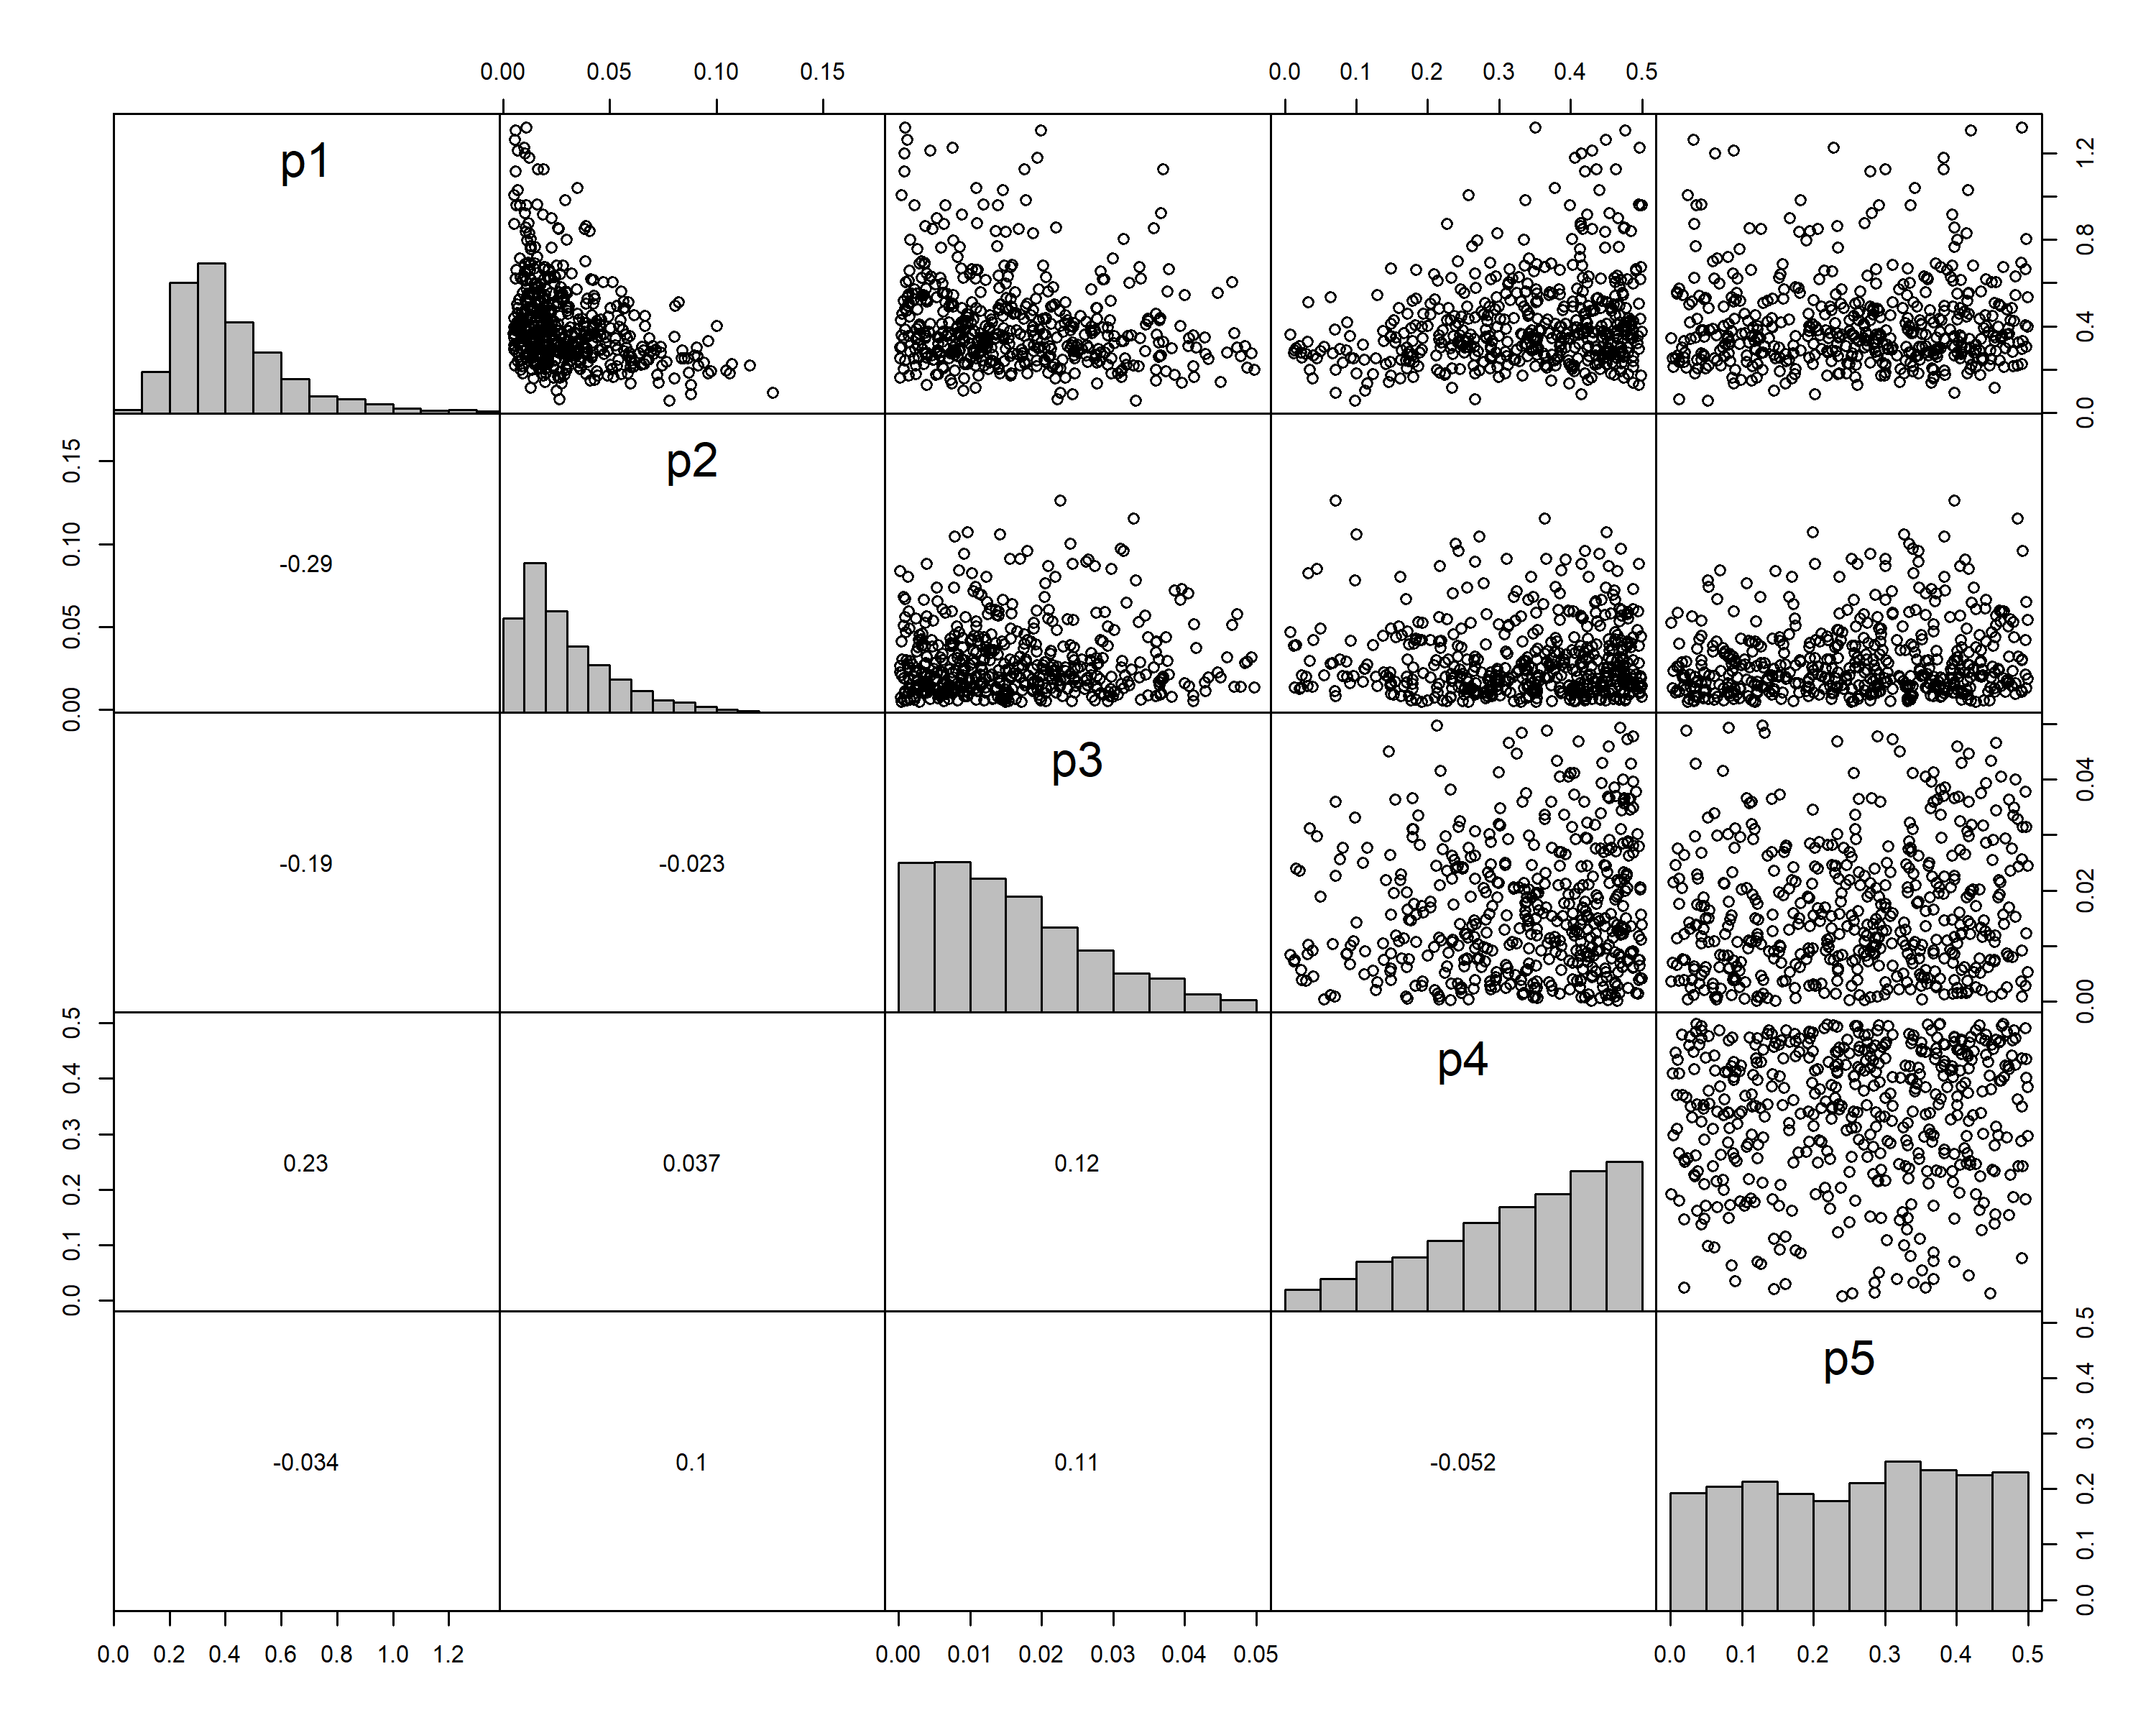
\includegraphics[width=1.0\textwidth]{figures/pairs_plot_Eifelgold.png} 
    \caption{Marginal posterior density and bivariate pairs plots for SoilR three-pool compartmental parameters ($k_f, k_i, k_s$, $\alpha_{fi}, \alpha_{is}$) from adaptive Metropolis MCMC sampling in Eifelgold plots.}
    \label{fig:pairs_plot_Eifelgold}
\end{figure}

\newpage

\begin{figure}[htbp]
    \centering
    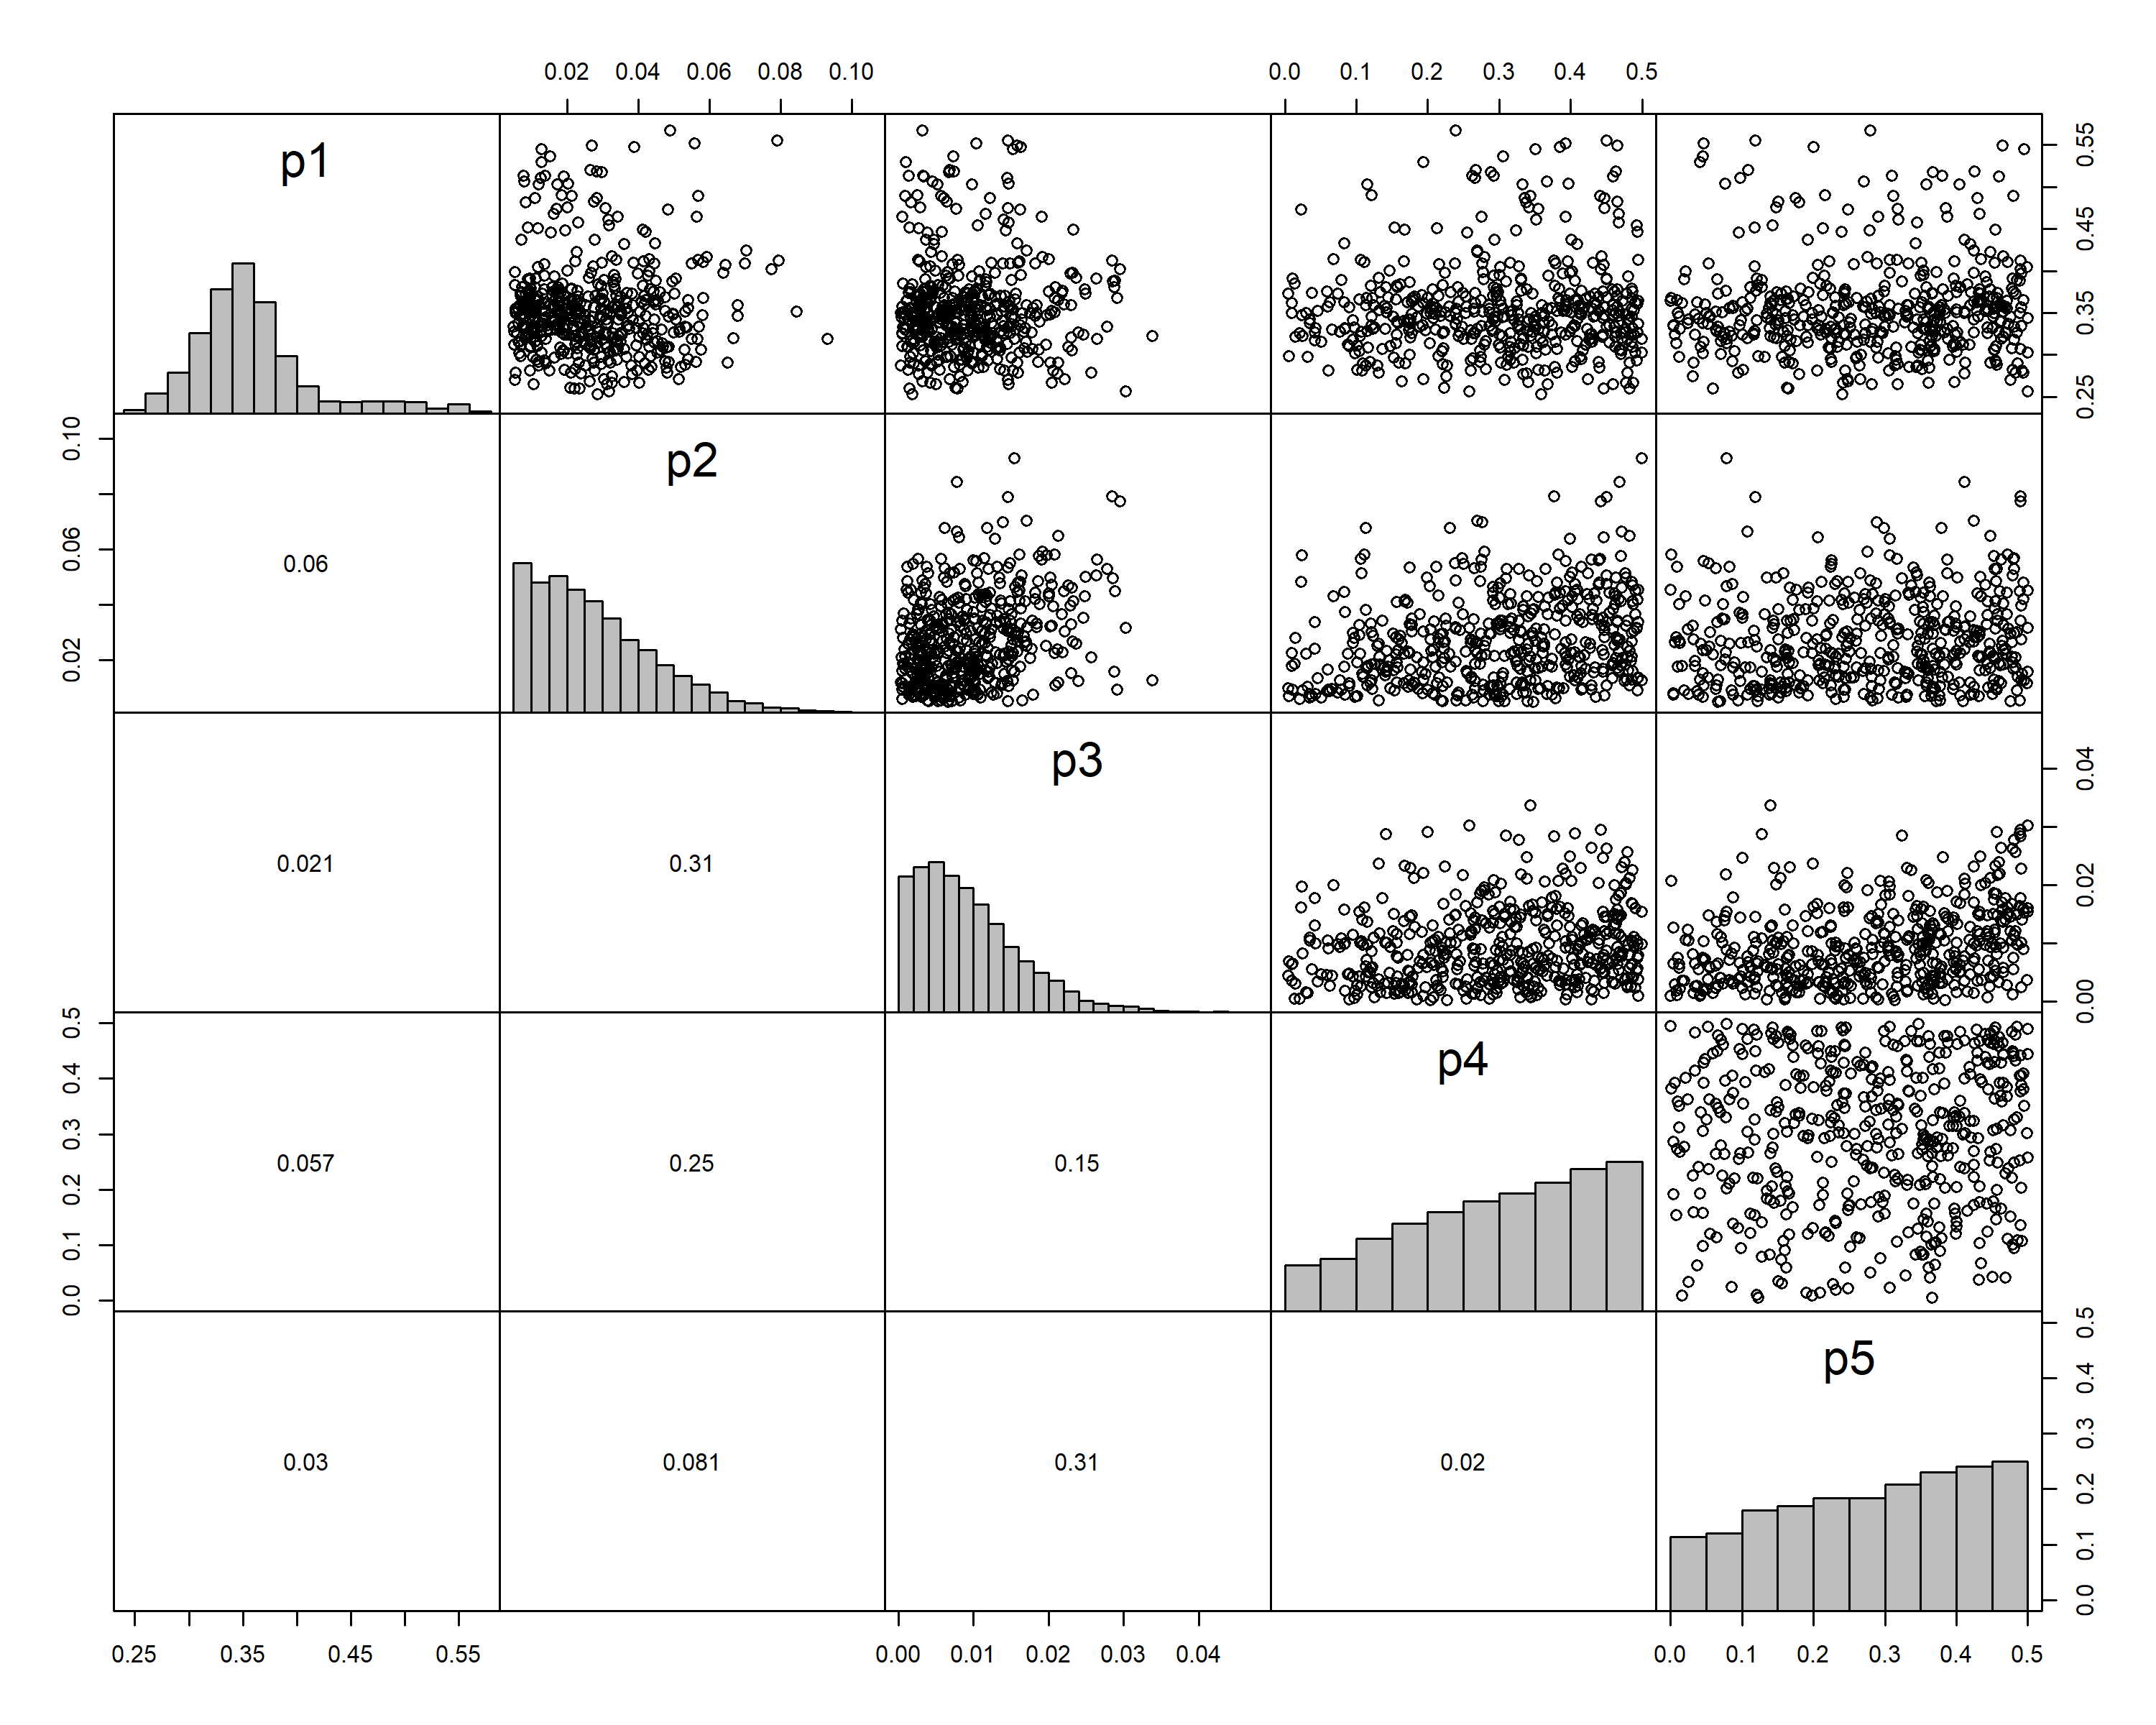
\includegraphics[width=1.0\textwidth]{figures/pairs_plot_Lime.png} 
    \caption{Marginal posterior density and bivariate pairs plots for SoilR three-pool compartmental parameters ($k_f, k_i, k_s$, $\alpha_{fi}, \alpha_{is}$) from adaptive Metropolis MCMC sampling in Lime plots.}
    \label{fig:pairs_plot_Lime}
\end{figure}

\newpage

% trace plots SoilR modeled pars
\begin{figure}[htbp]
    \centering
    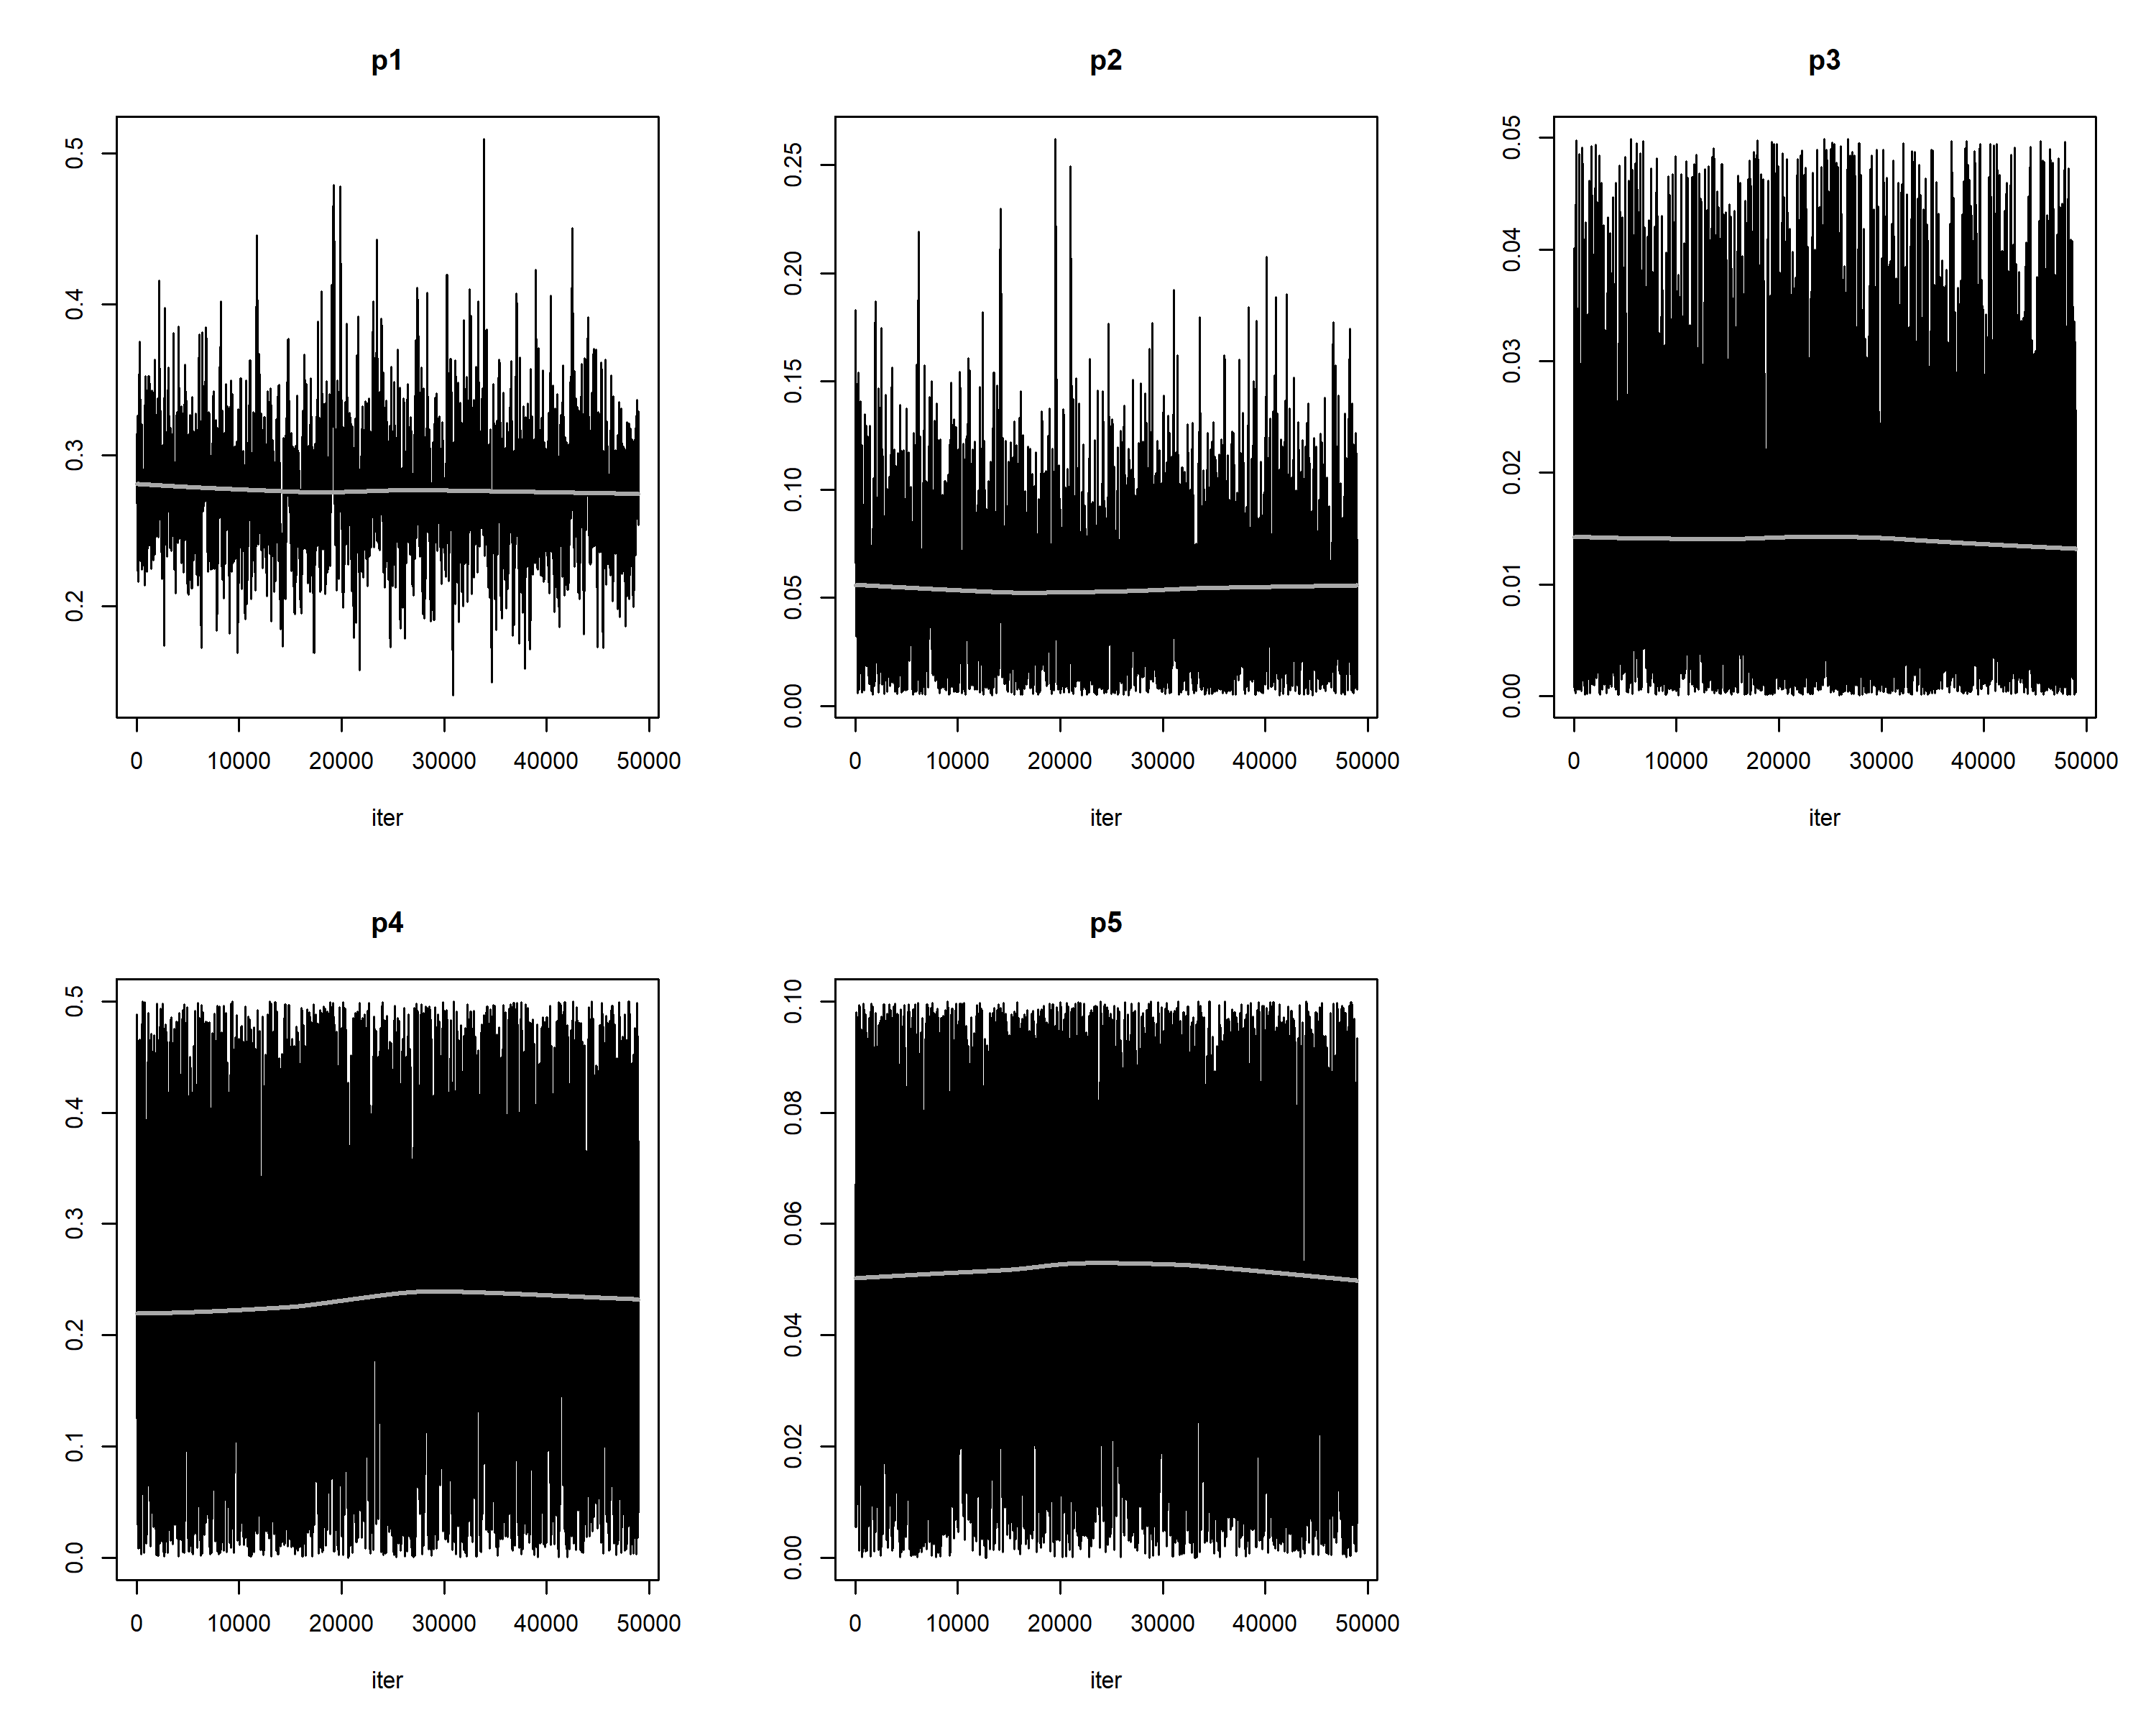
\includegraphics[width=1.0\textwidth]{figures/convergence_plot_control.png} 
    \caption{MCMC trace and convergence diagnostics for SoilR three-pool model parameters in Control plots.}
    \label{fig:convergence_plot_control}
\end{figure}

\newpage

\begin{figure}[htbp]
    \centering
    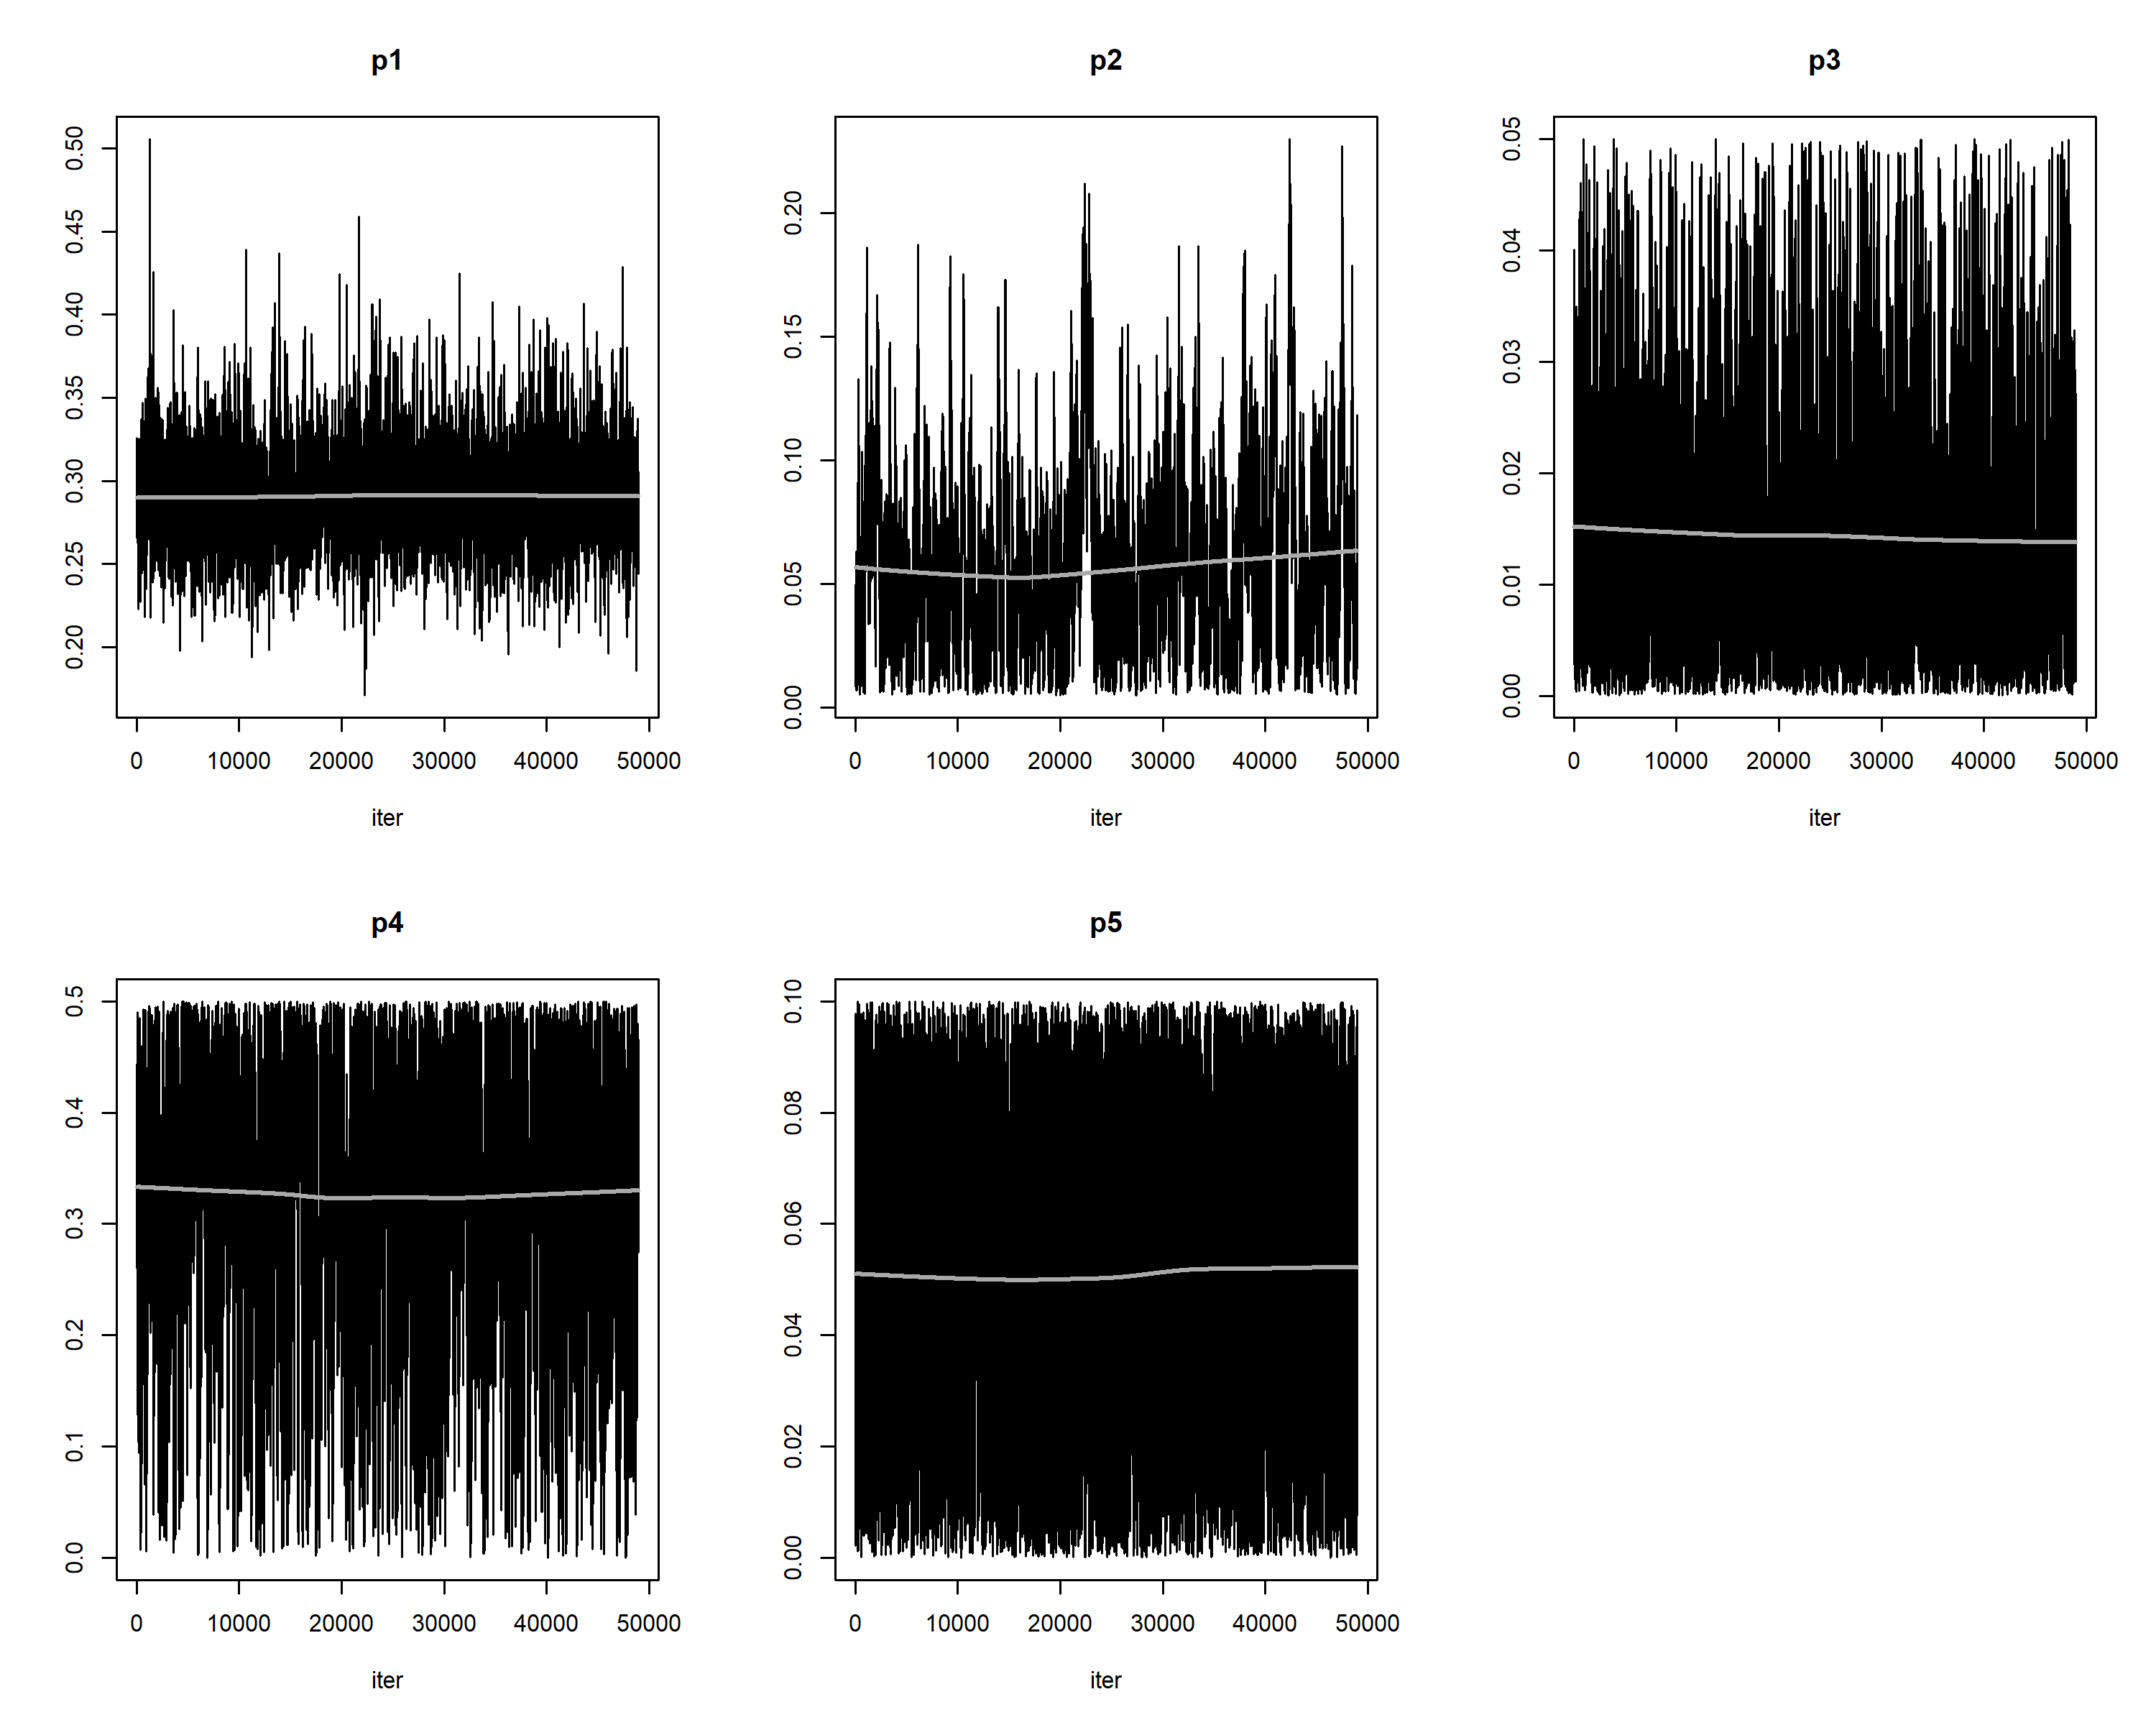
\includegraphics[width=1.0\textwidth]{figures/convergence_plot_Bolsdorfer.png} 
    \caption{MCMC trace and convergence diagnostics for SoilR three-pool model parameters in Bolsdorfer basalt plots.}
    \label{fig:convergence_plot_Bolsdorfer}
\end{figure}

\newpage

\begin{figure}[htbp]
    \centering
    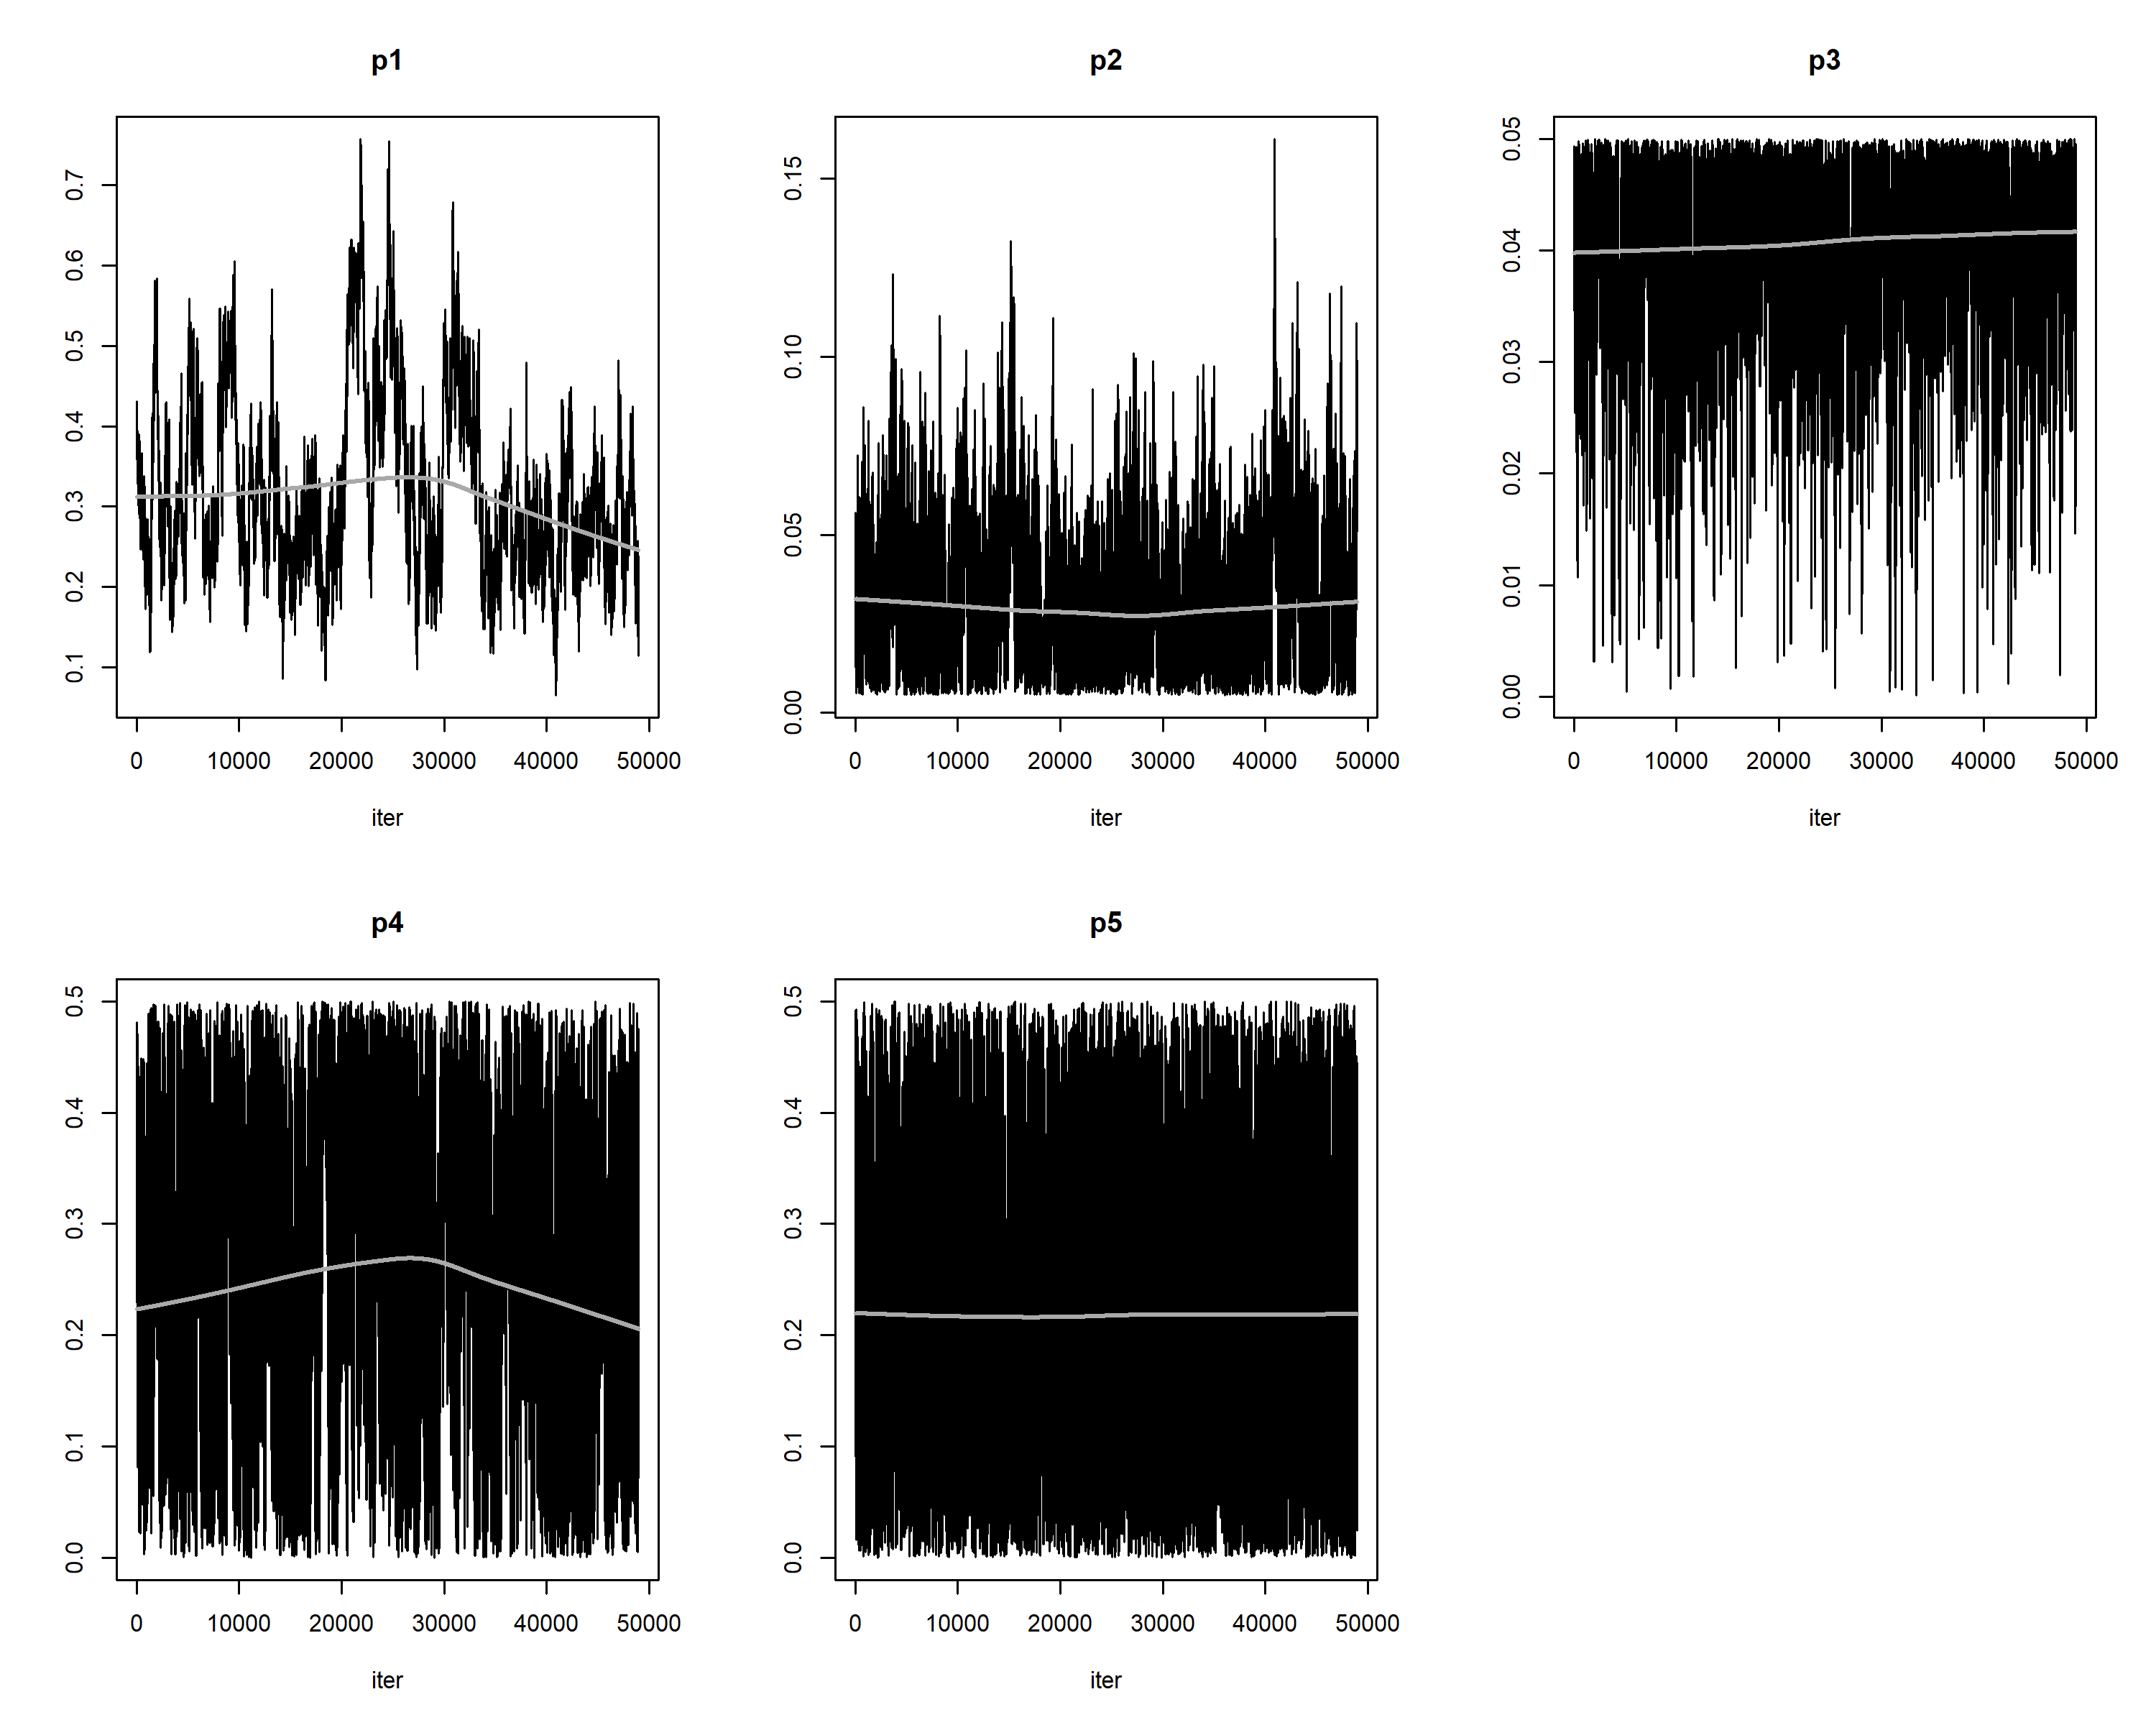
\includegraphics[width=1.0\textwidth]{figures/convergence_plot_Huhnerberg.png} 
    \caption{MCMC trace and convergence diagnostics for SoilR three-pool model parameters in Hühnerberg basalt plots.}
    \label{fig:convergence_plot_Huhnerberg}
\end{figure}

\newpage

\begin{figure}[htbp]
    \centering
    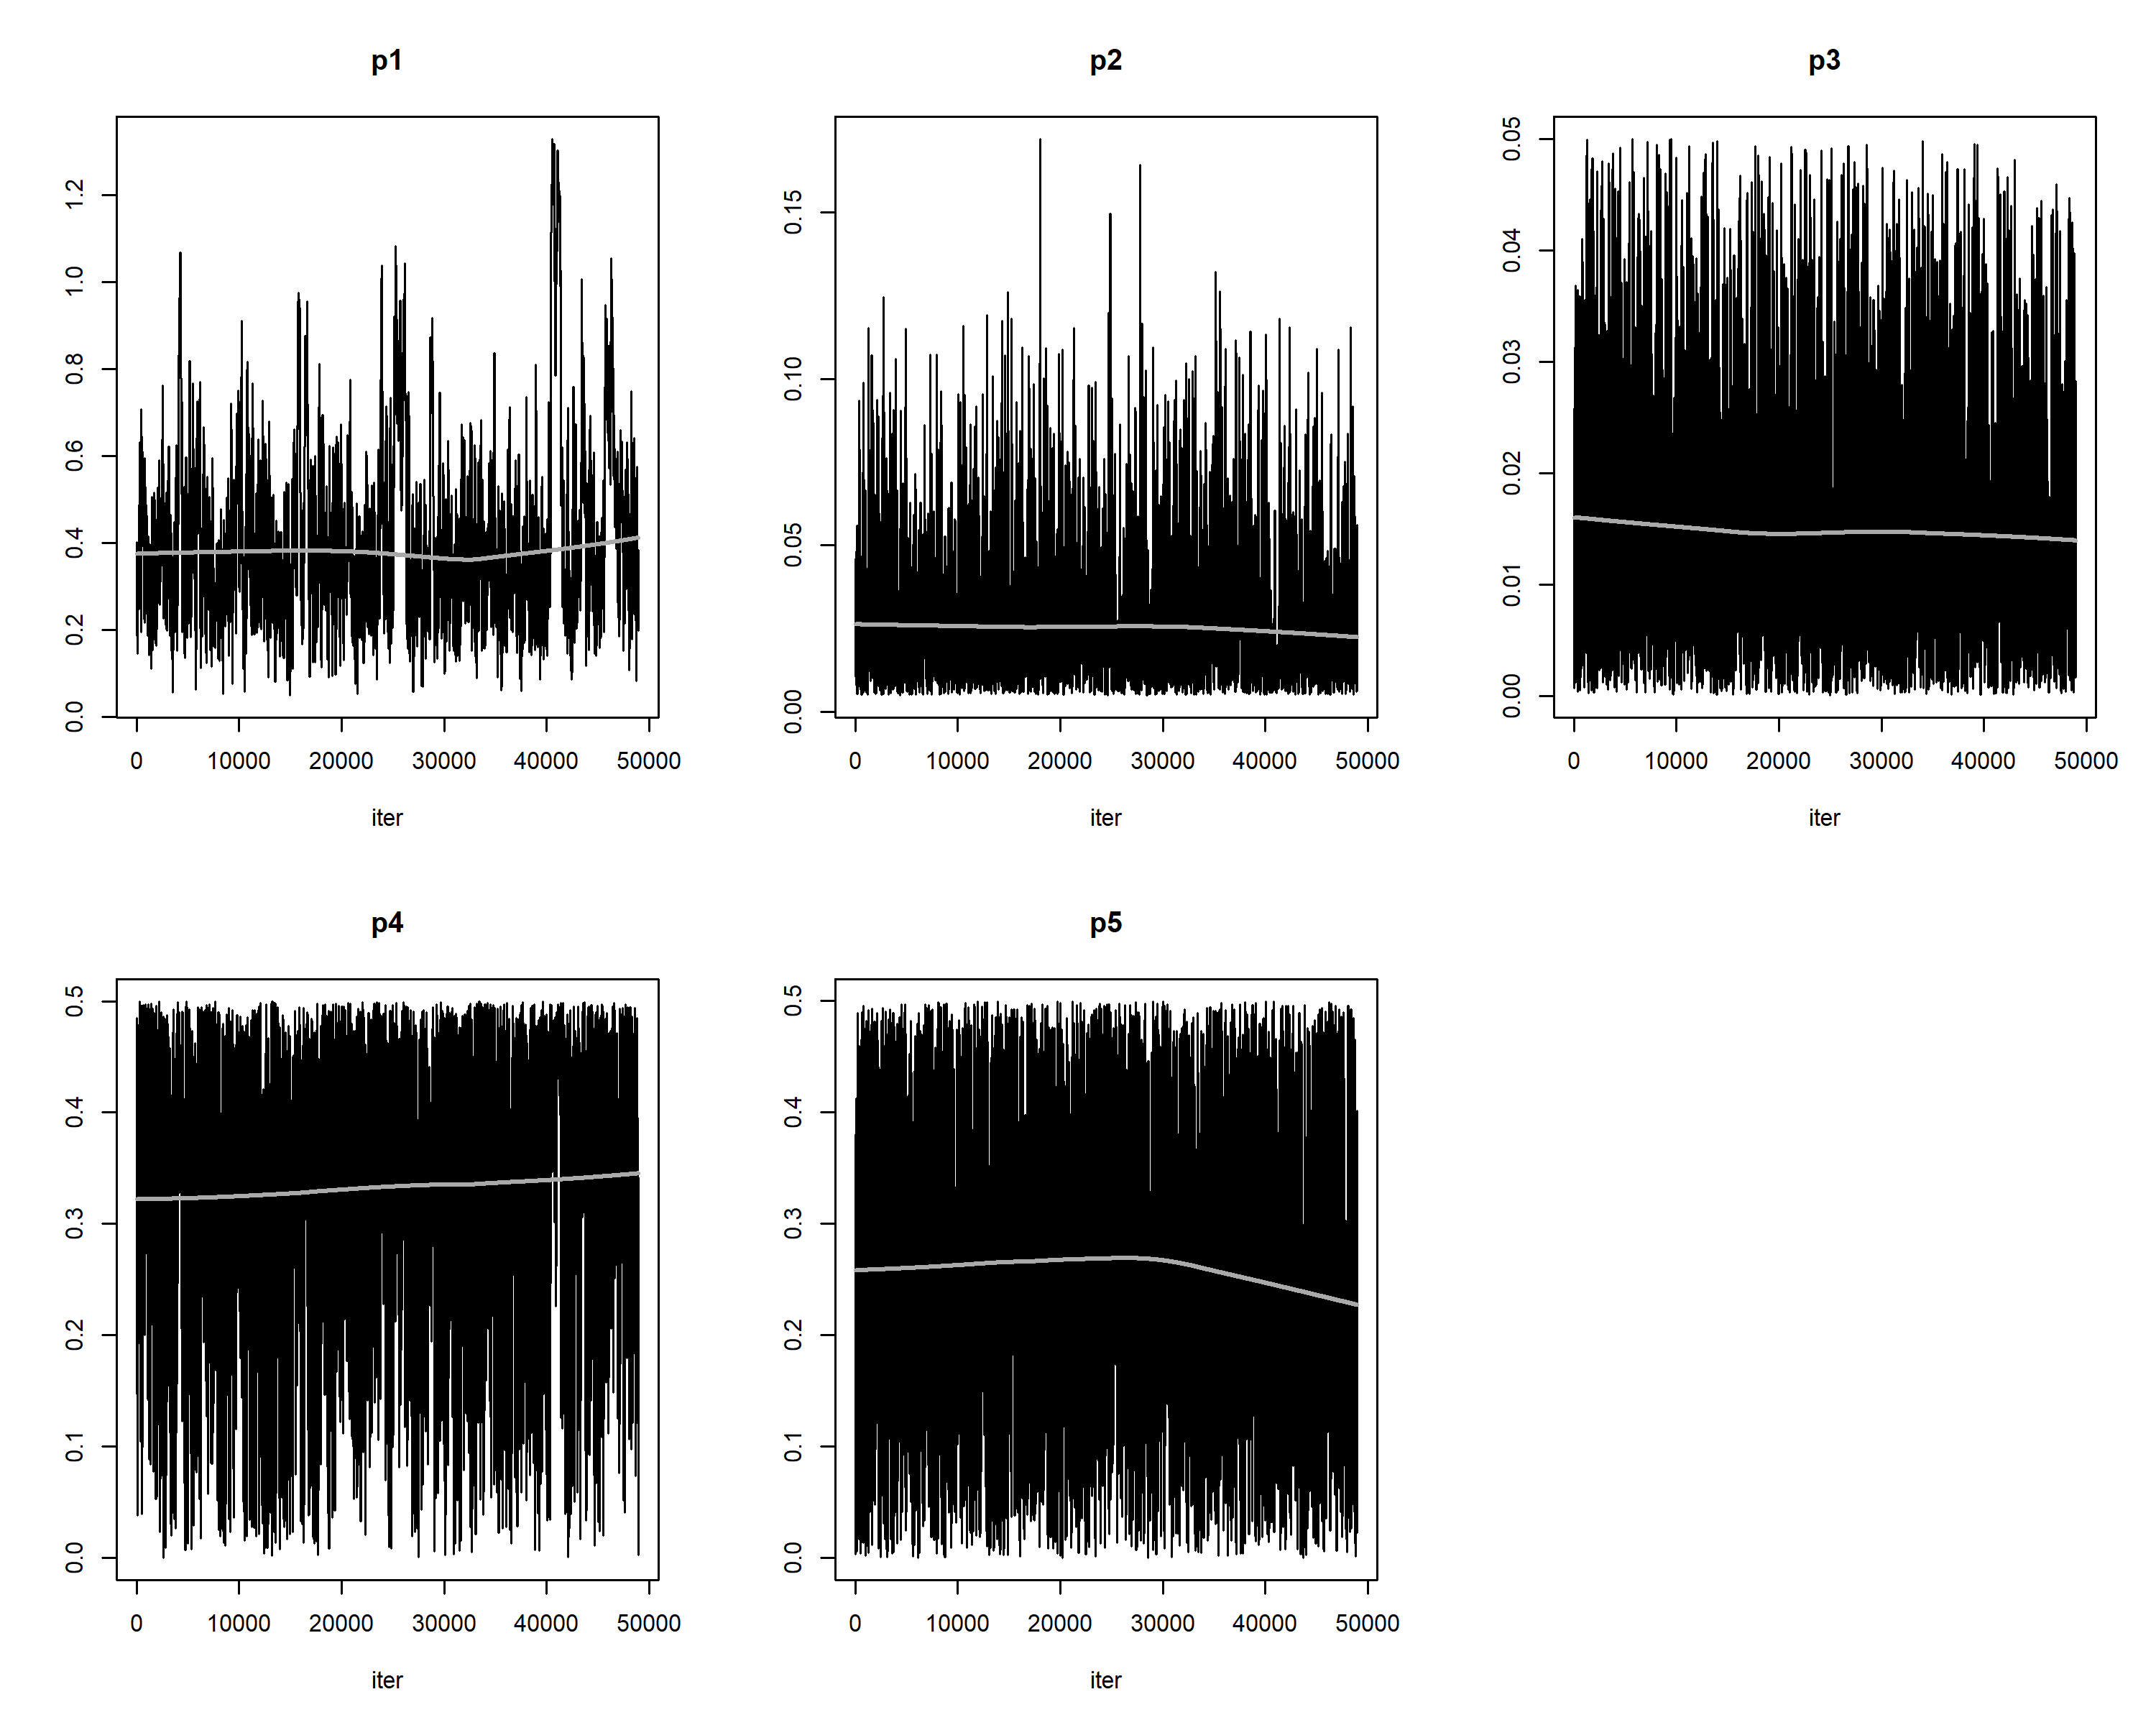
\includegraphics[width=1.0\textwidth]{figures/convergence_plot_Eifelgold.png} 
    \caption{MCMC trace and convergence diagnostics for SoilR three-pool model parameters in Eifelgold tephrite plots.}
    \label{fig:convergence_plot_Eifelgold}
\end{figure}

\newpage

\begin{figure}[htbp]
    \centering
    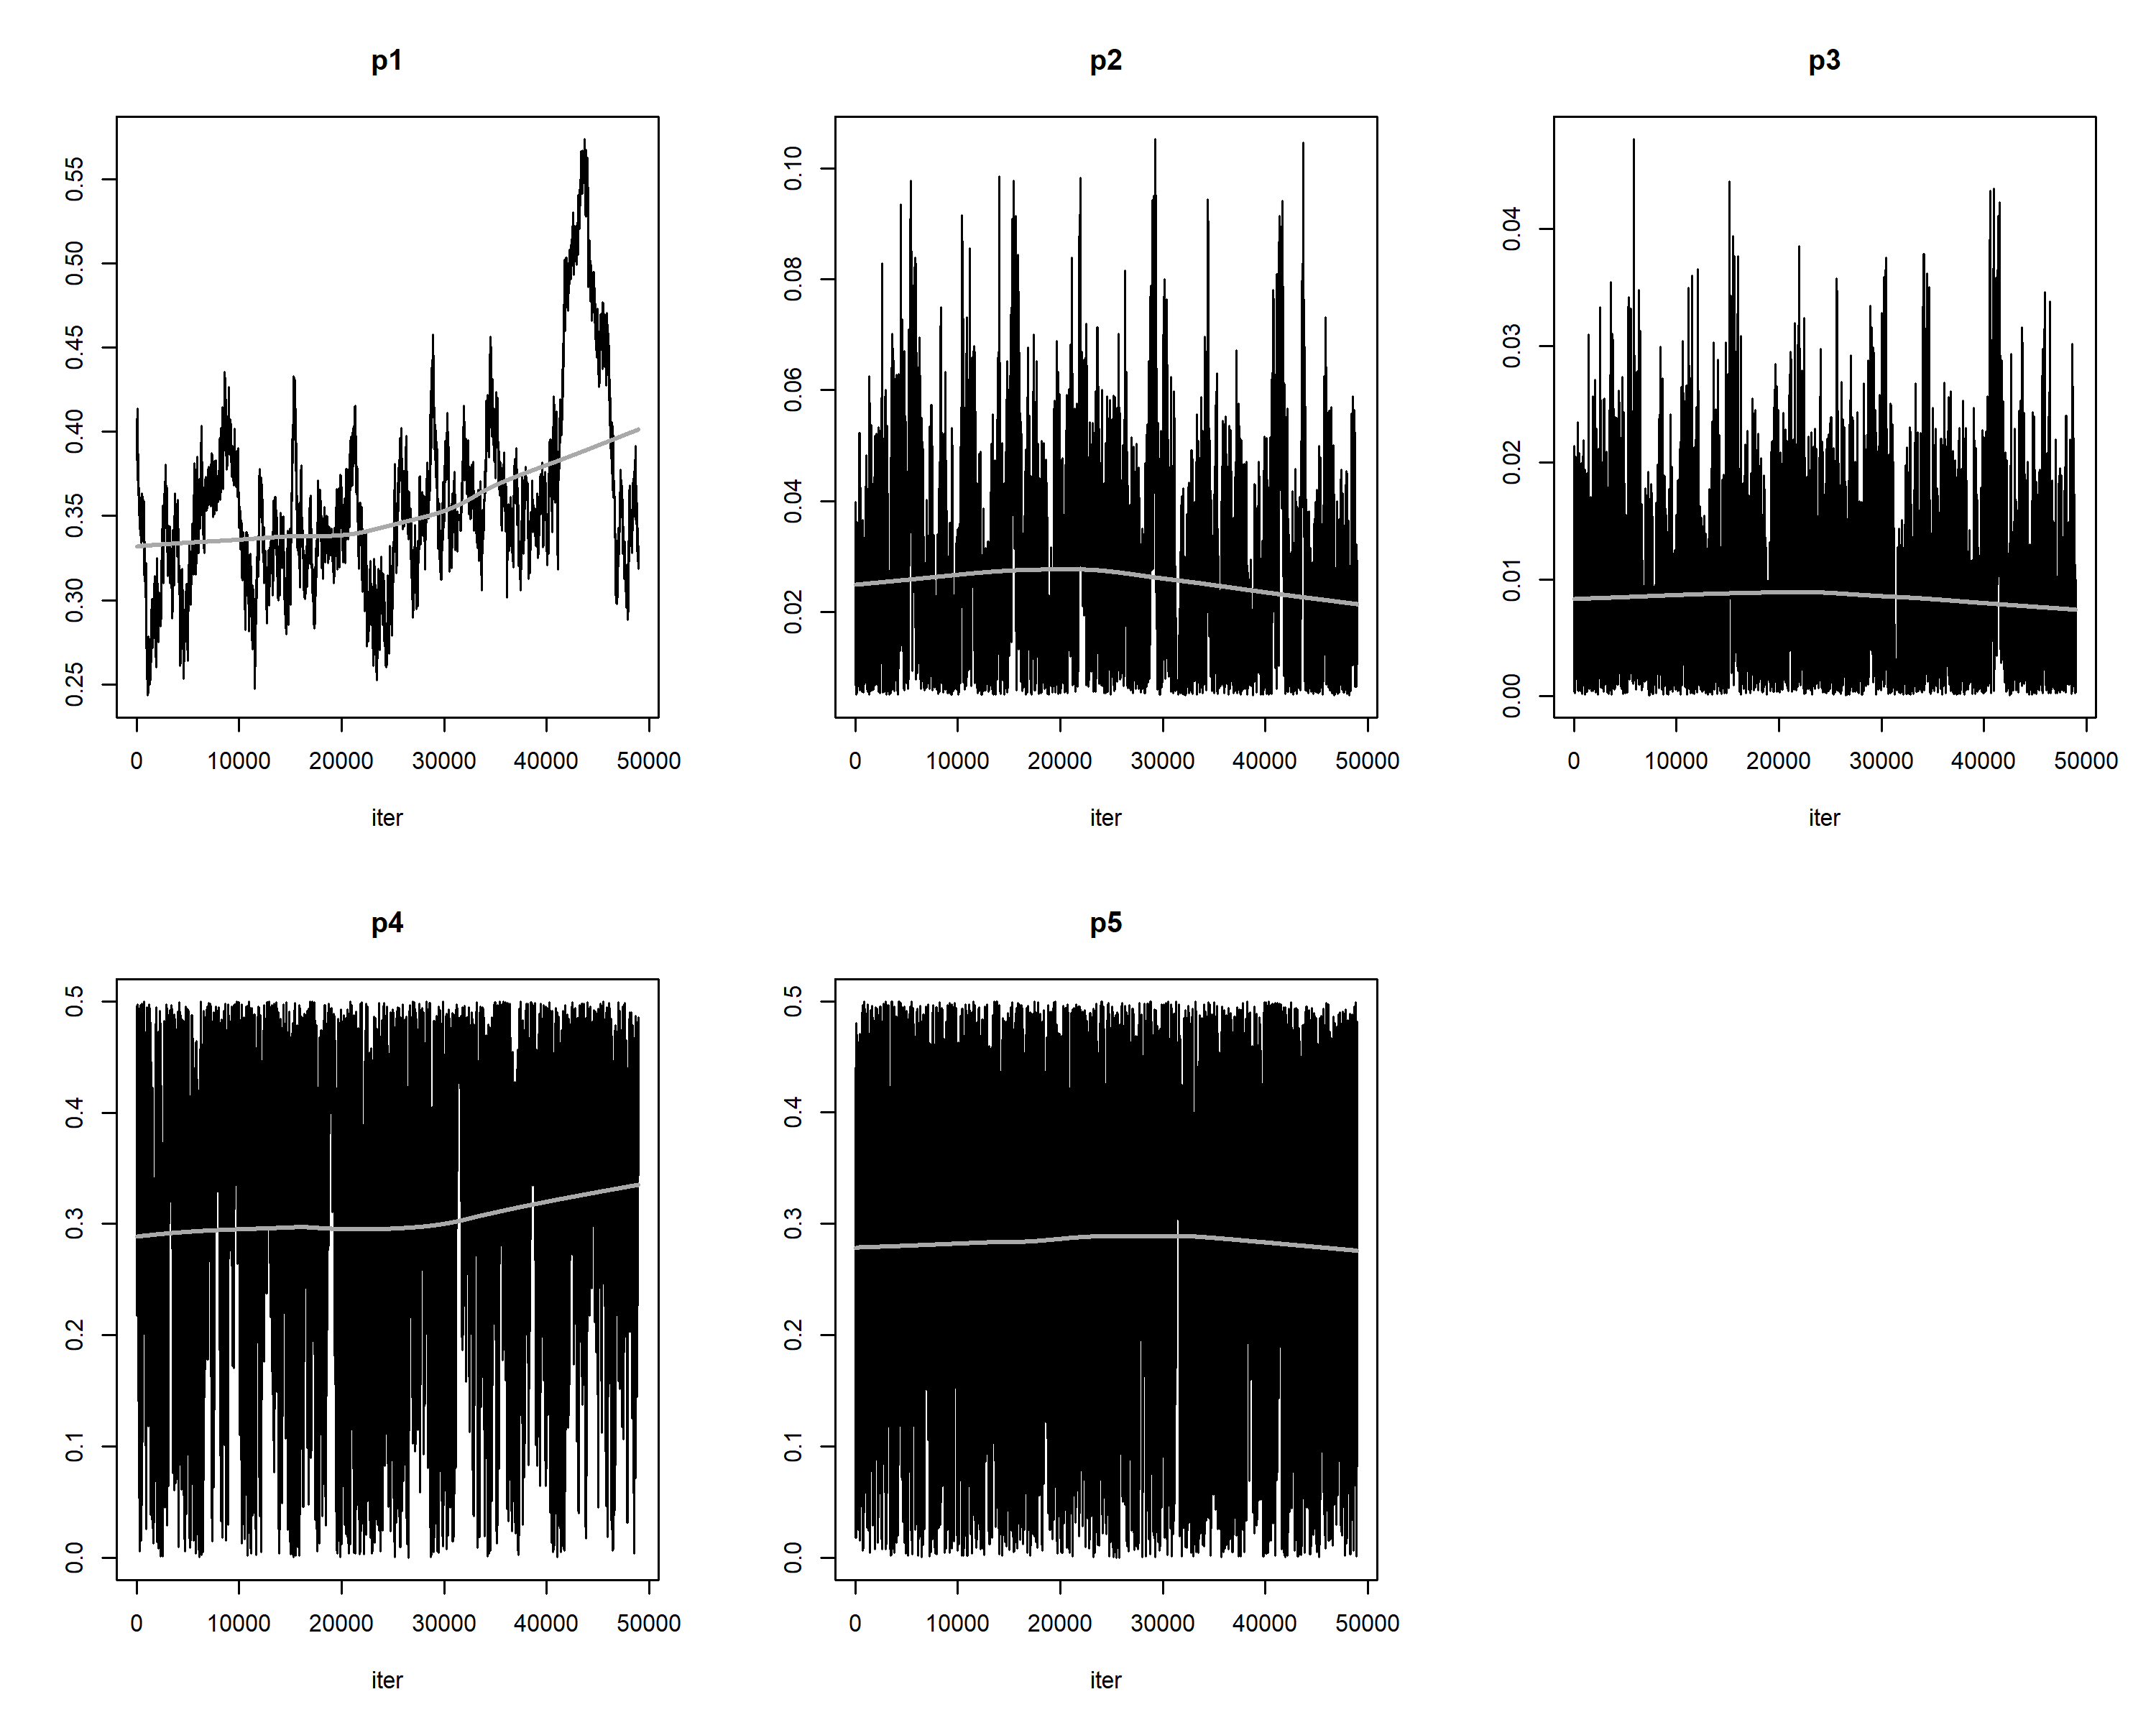
\includegraphics[width=1.0\textwidth]{figures/convergence_plot_Lime.png} 
    \caption{MCMC trace and convergence diagnostics for SoilR three-pool model parameters in Lime plots.}
    \label{fig:convergence_plot_Lime}
\end{figure}

\newpage
  
% posterior distributions of modeled SoilR pars
  
\begin{figure}[htbp]
    \centering
    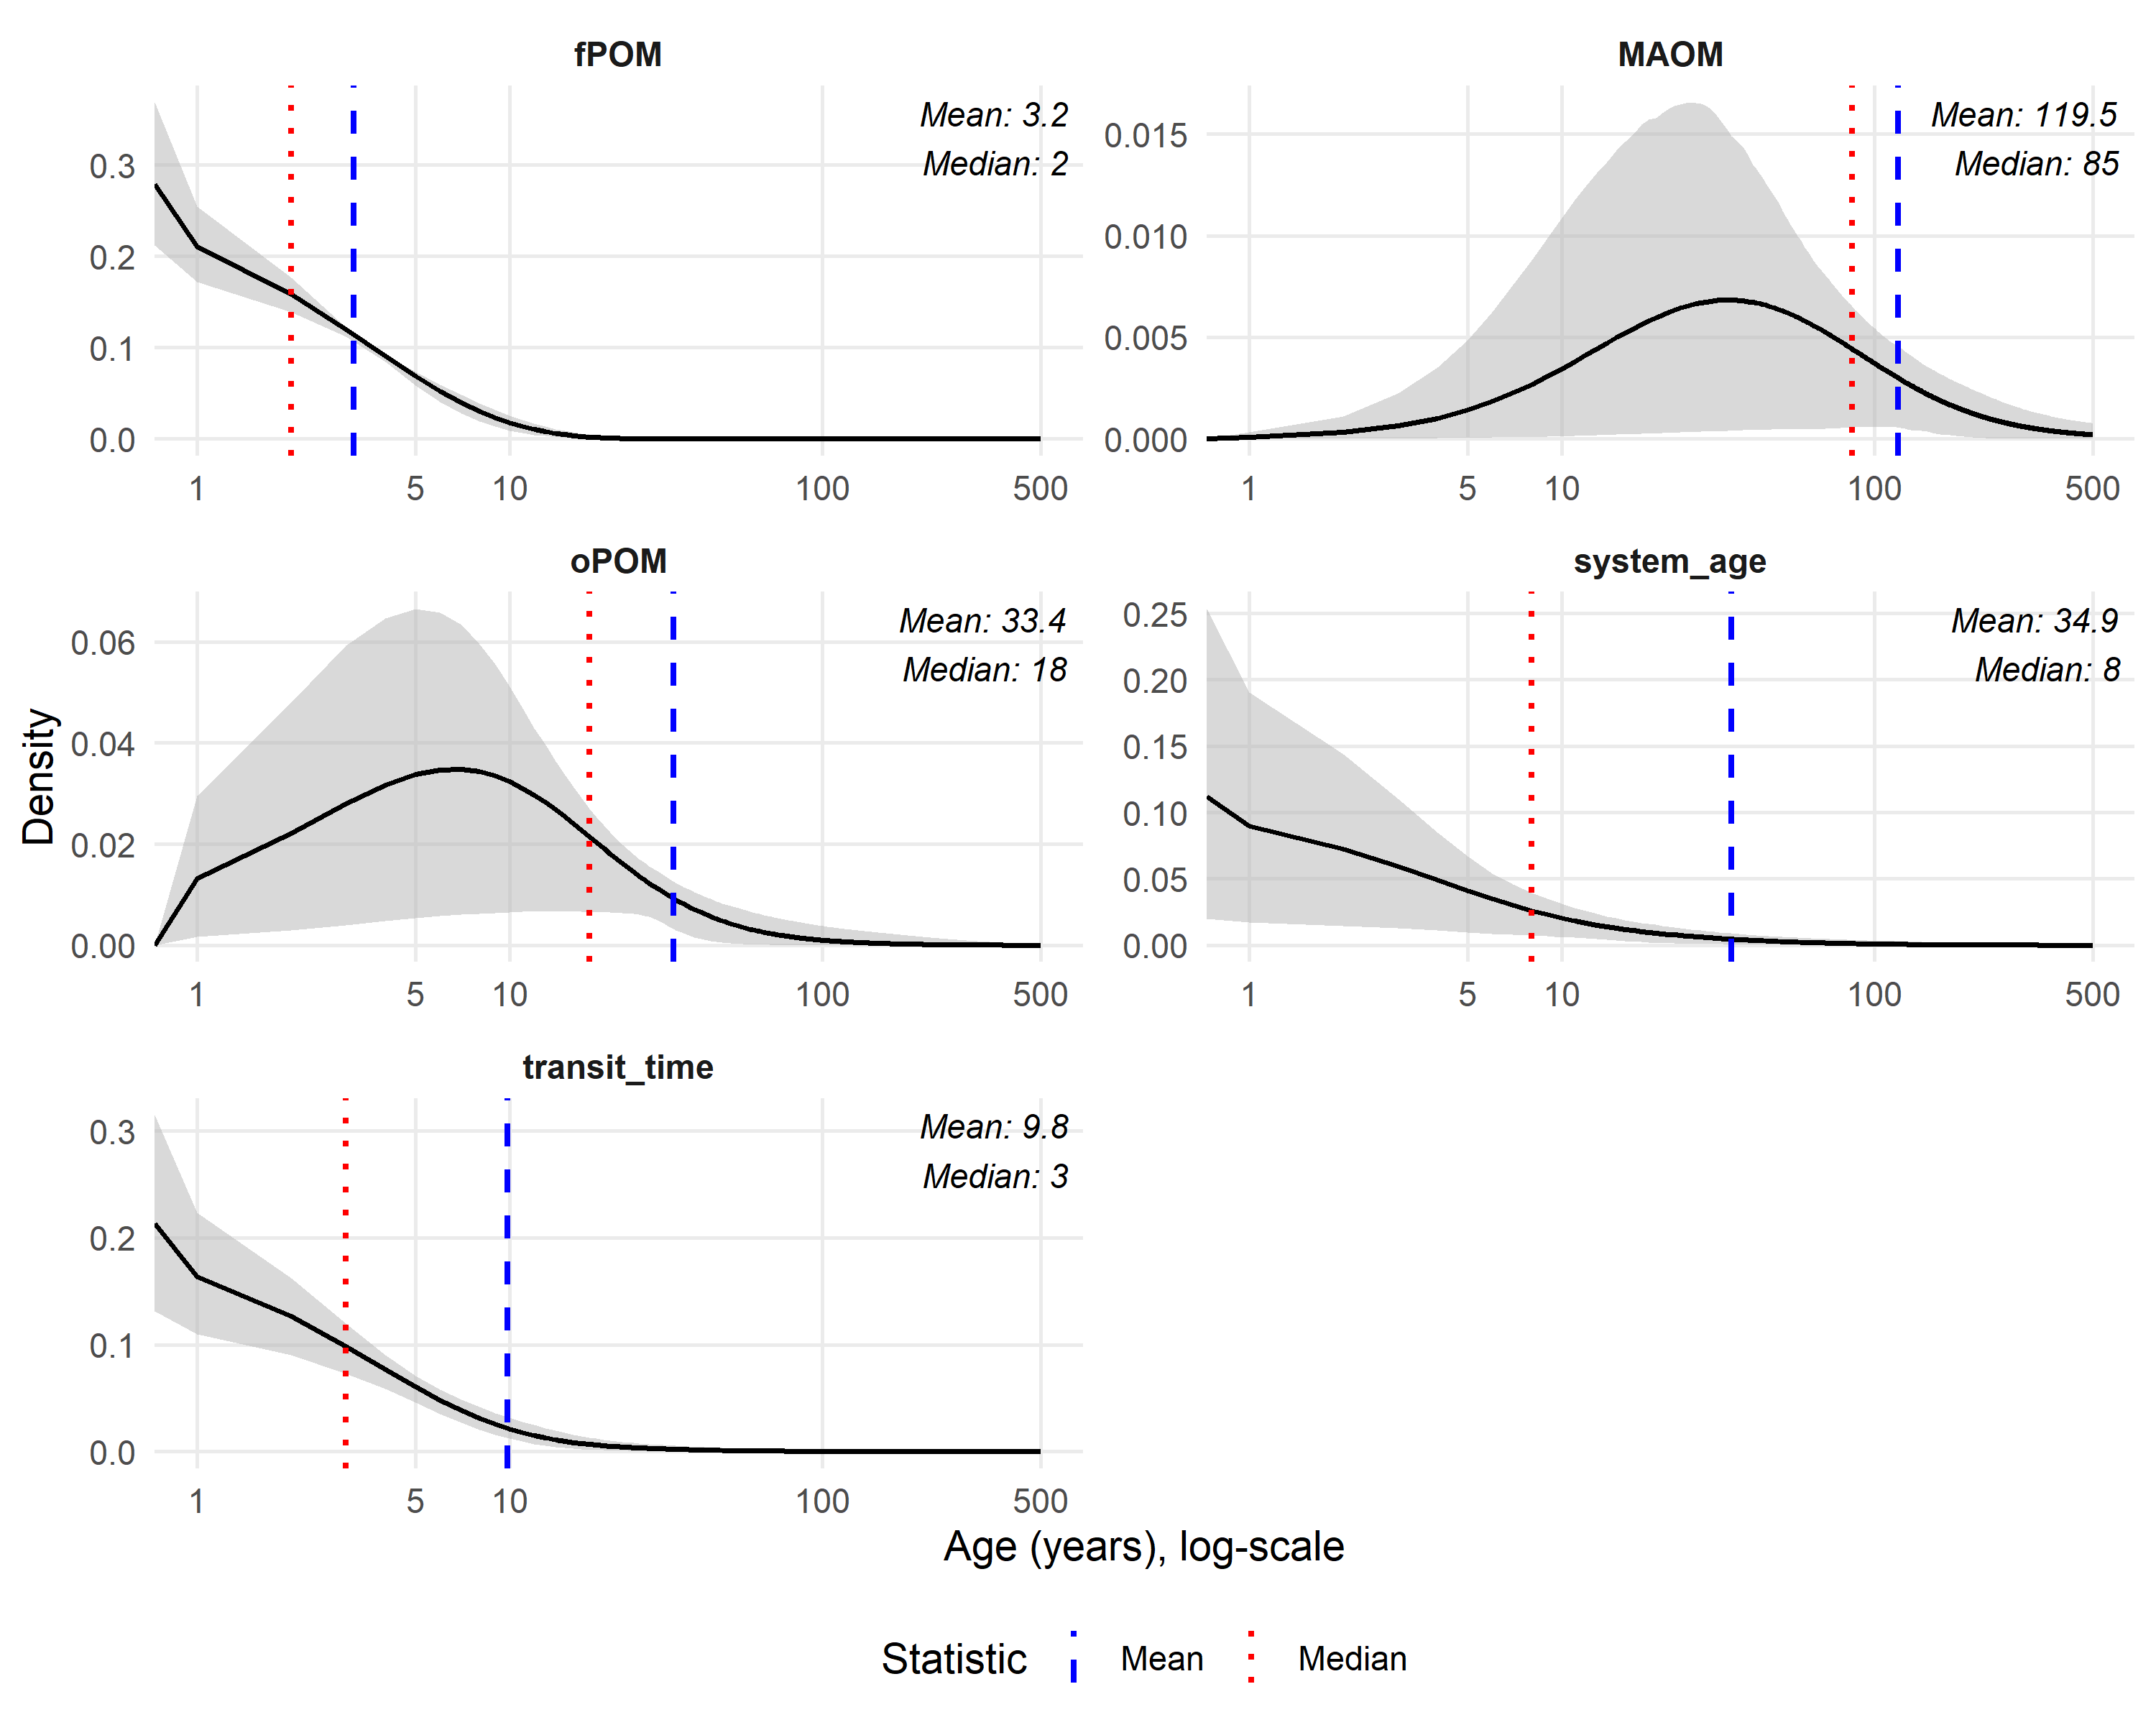
\includegraphics[width=1.0\textwidth]{figures/plot_log_age_tt_control.png} 
    \caption{Posterior distributions of SoilR-derived pool ages (fPOM, oPOM, MAOM) and whole-system carbon transit time (0--500 yr horizon) in control soil.}
    \label{fig:plot_log_age_tt_control}
\end{figure}

\newpage

\begin{figure}[htbp]
    \centering
    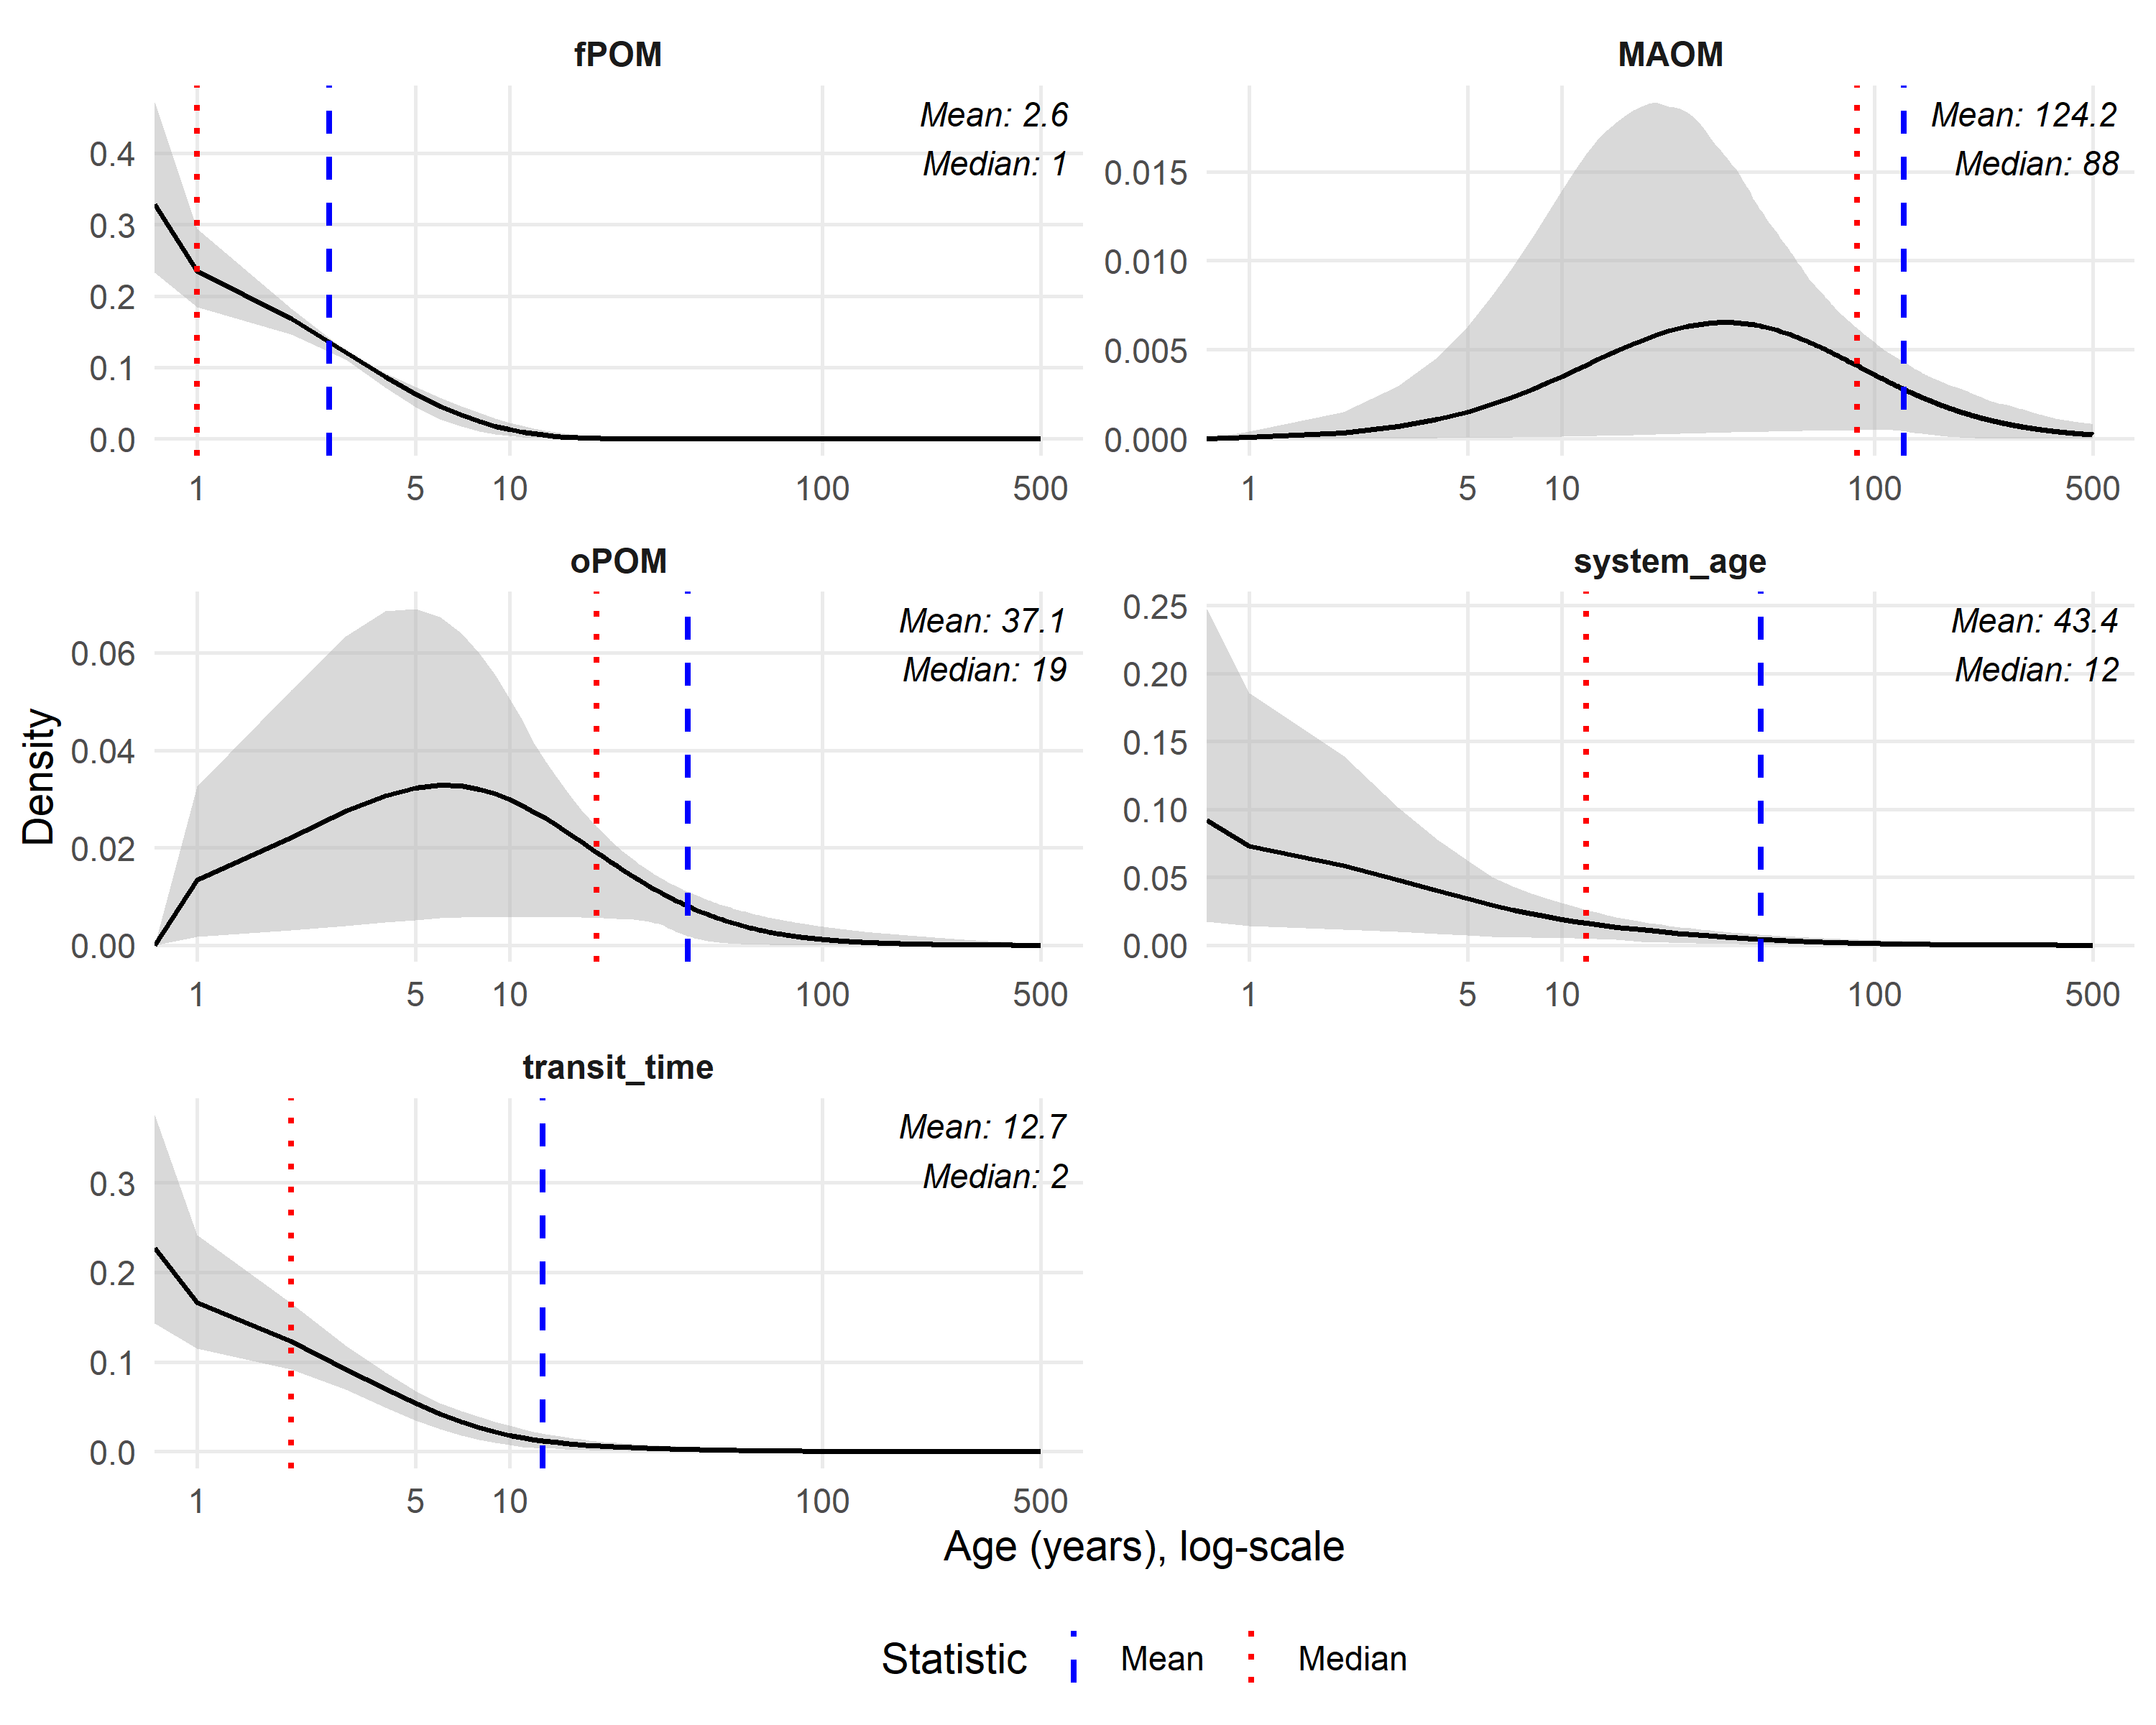
\includegraphics[width=1.0\textwidth]{figures/plot_log_age_tt_Bolsdorfer.png} 
    \caption{Posterior distributions of SoilR-derived pool ages (fPOM, oPOM, MAOM) and whole-system carbon transit time (0--500 yr horizon) in soil amended with Bolsdorfer basalt.}
    \label{fig:plot_log_age_tt_Bolsdorfer}
\end{figure}

\newpage

\begin{figure}[htbp]
    \centering
    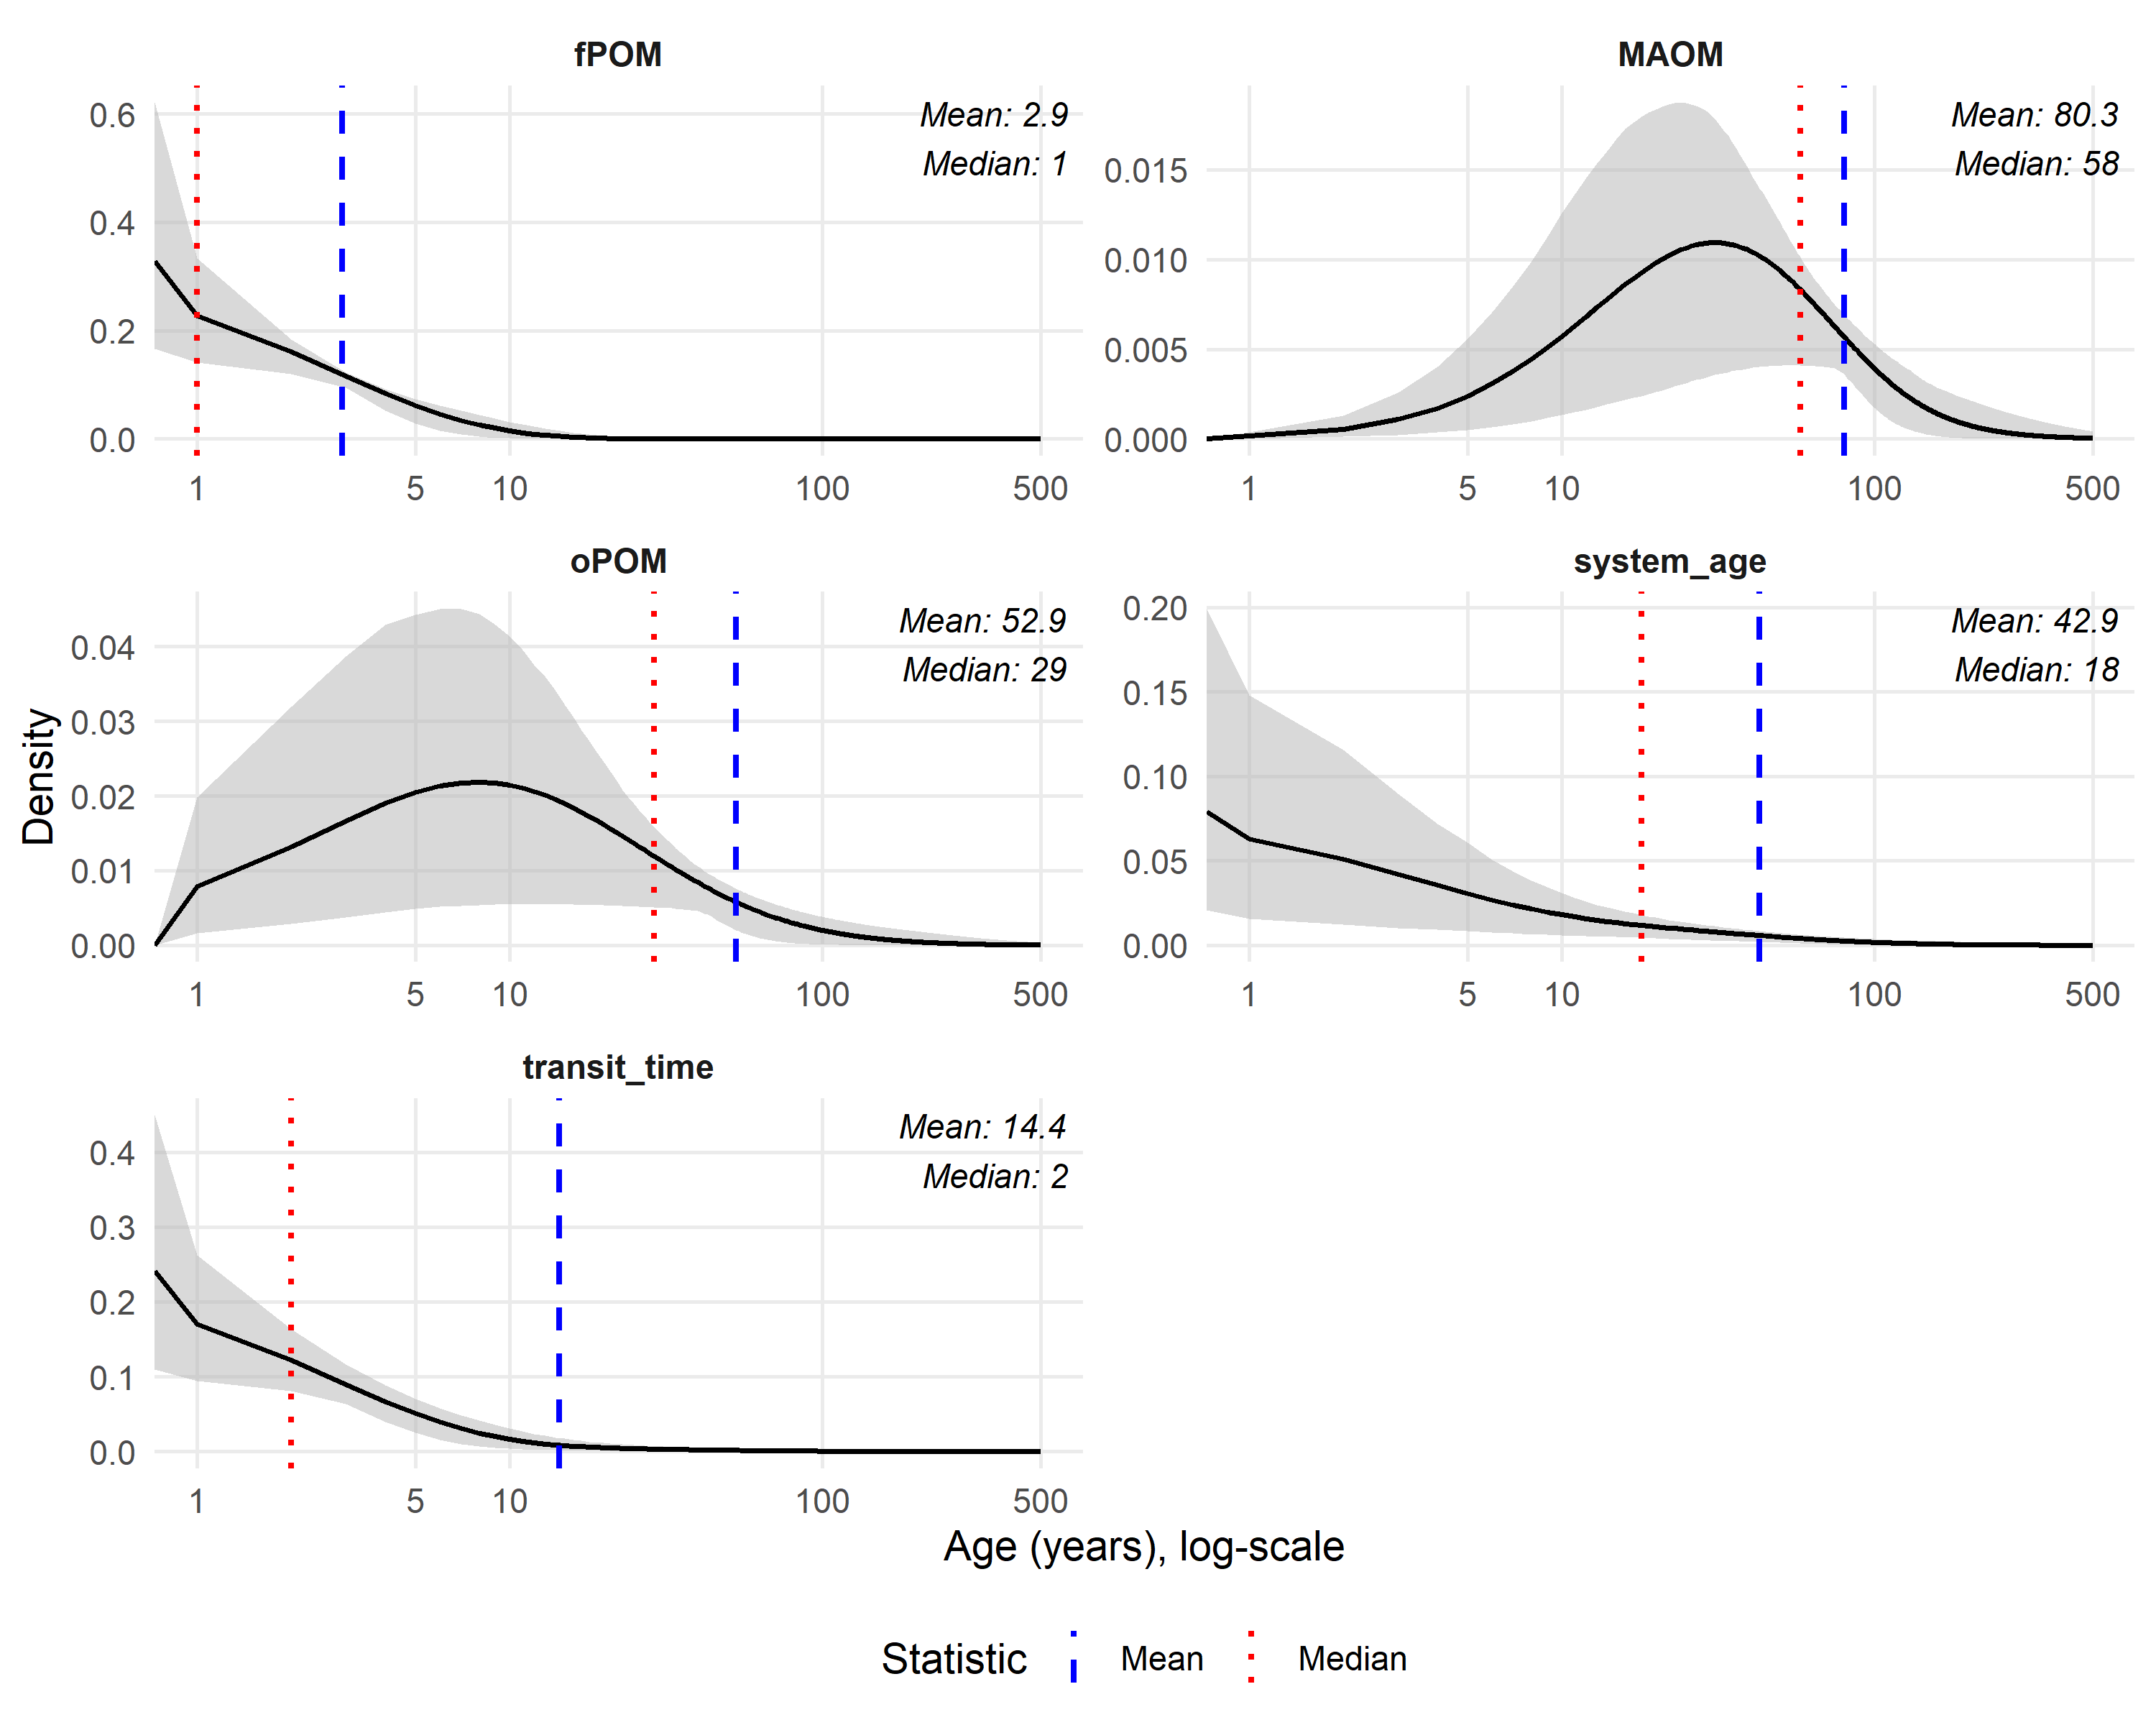
\includegraphics[width=1.0\textwidth]{figures/plot_log_age_tt_Huhnerberg.png} 
    \caption{Posterior distributions of SoilR-derived pool ages (fPOM, oPOM, MAOM) and whole-system carbon transit time (0--500 yr horizon) in soil amended with Hühnerberg basalt.}
    \label{fig:plot_log_age_tt_Huhnerberg}
\end{figure}

\newpage

\begin{figure}[htbp]
    \centering
    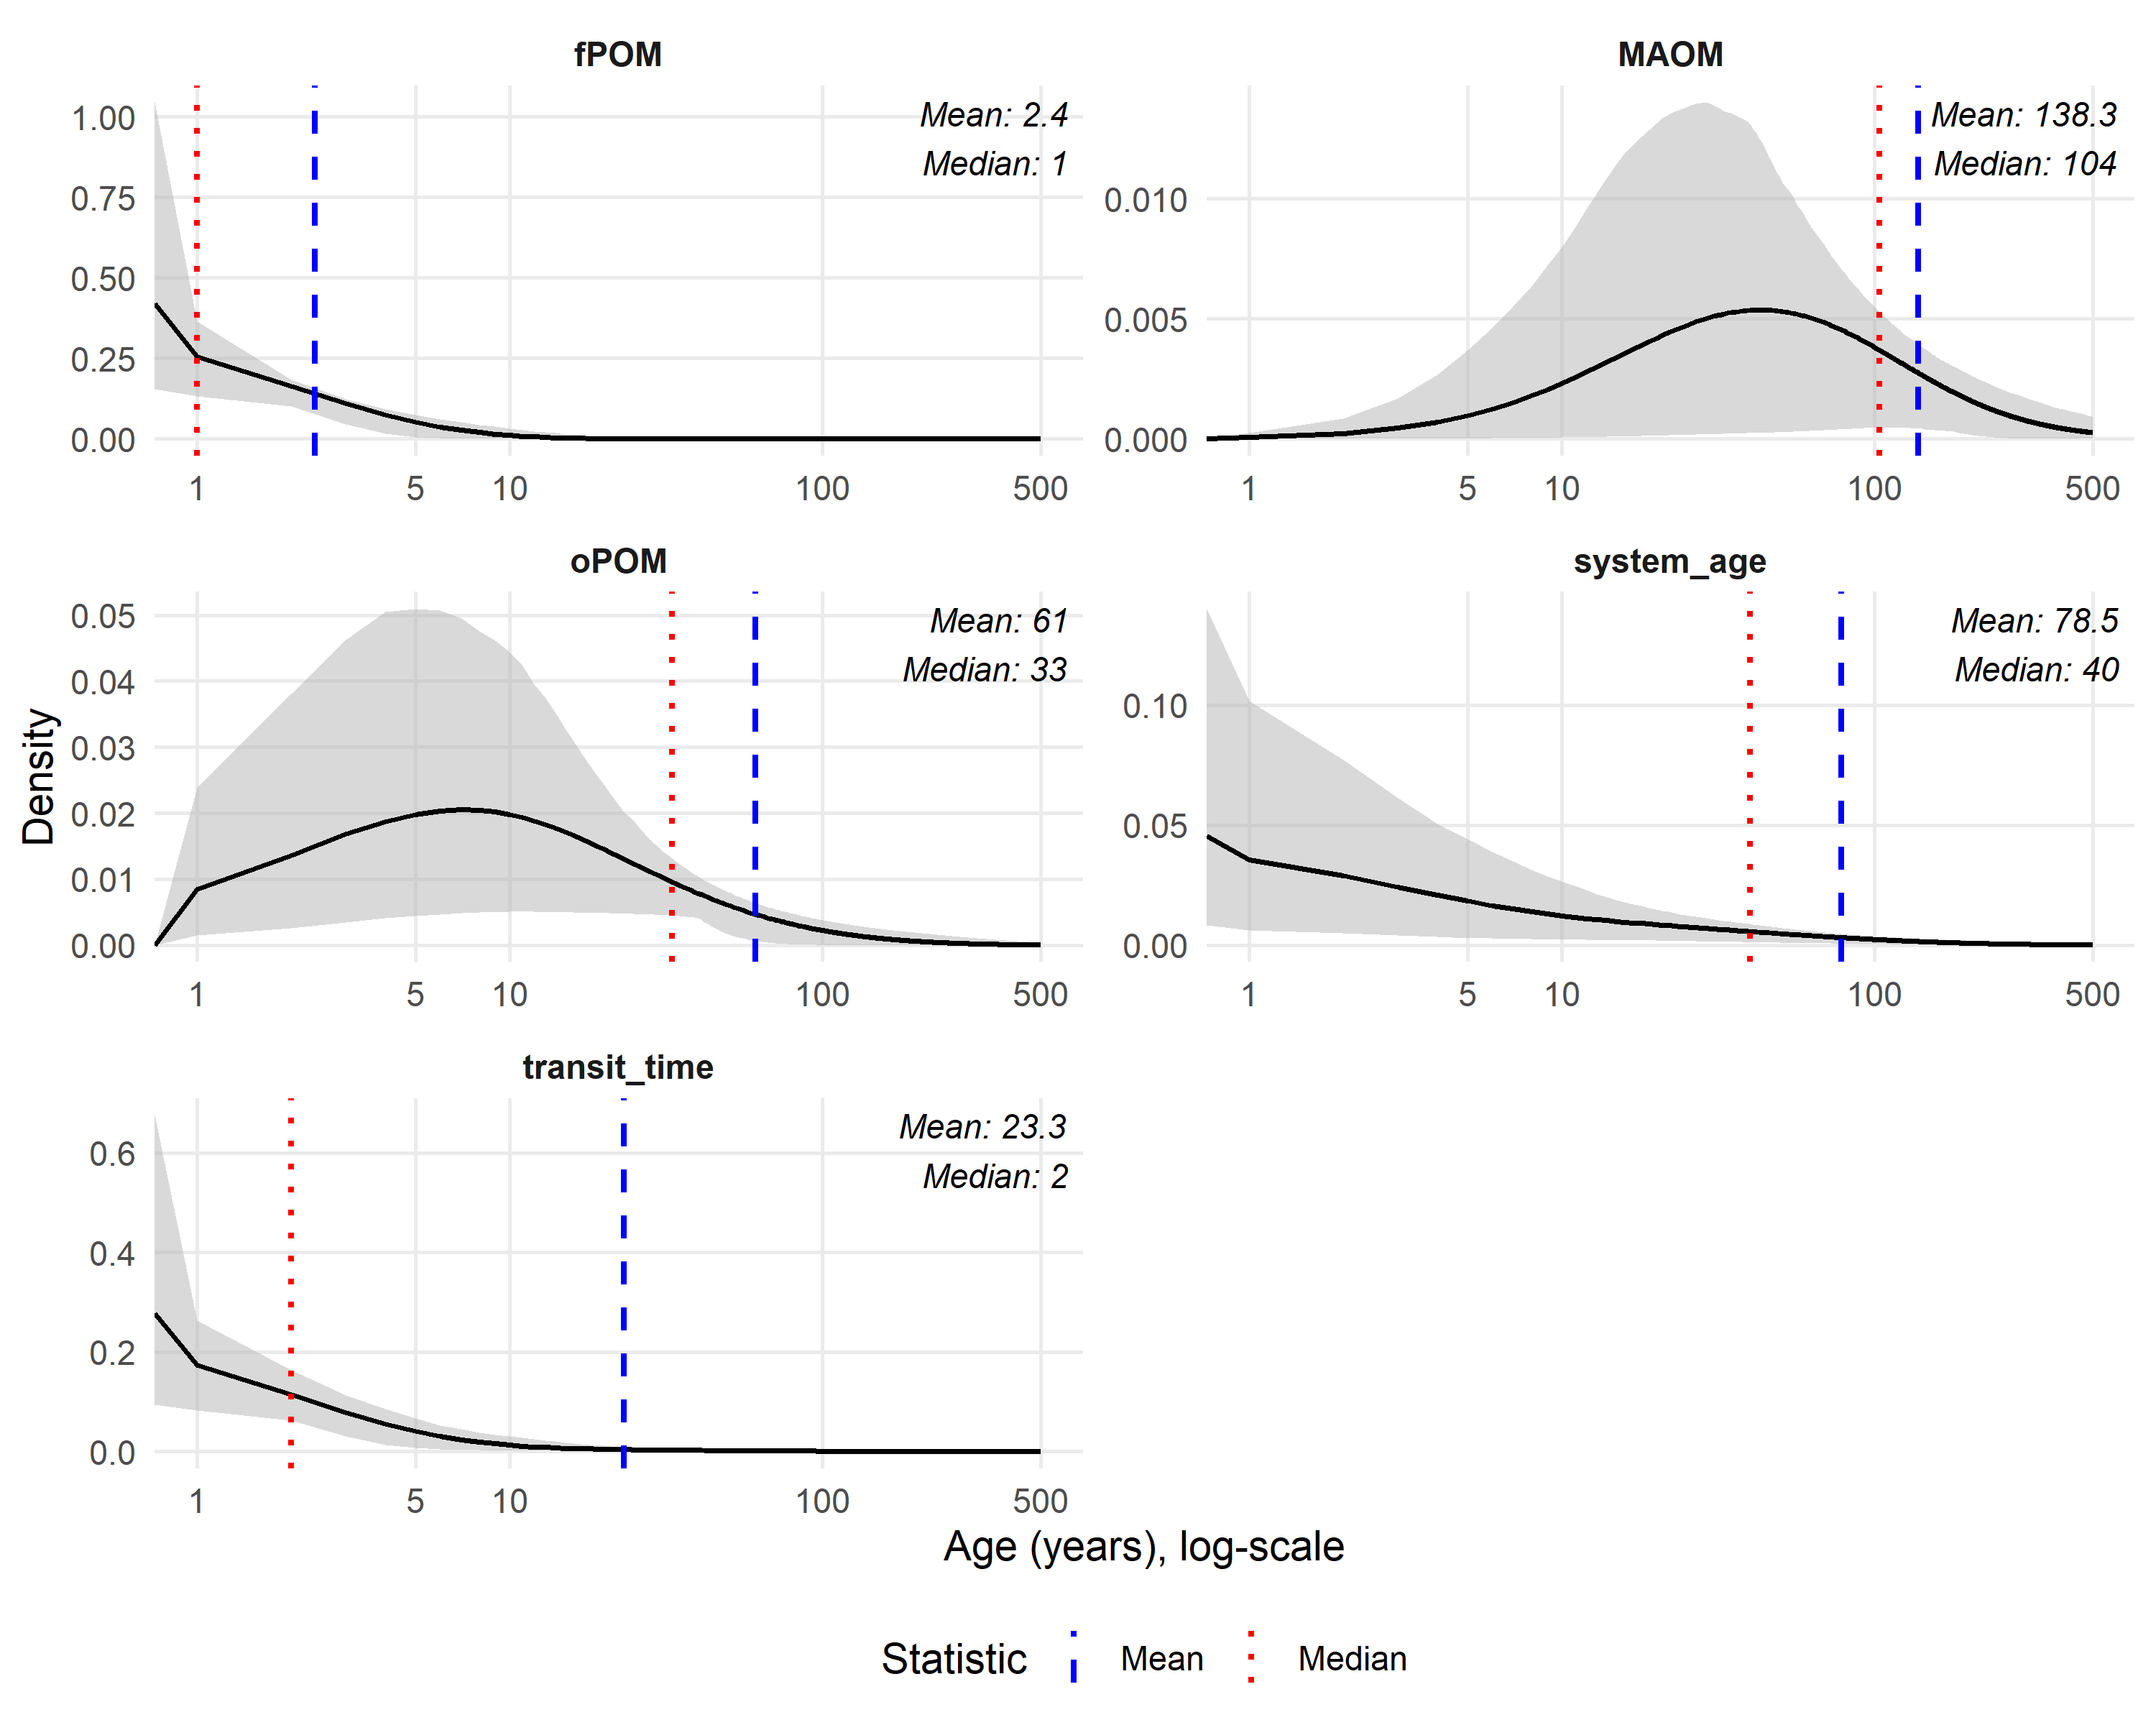
\includegraphics[width=1.0\textwidth]{figures/plot_log_age_tt_Eifelgold.png} 
    \caption{Posterior distributions of SoilR-derived pool ages (fPOM, oPOM, MAOM) and whole-system carbon transit time (0--500 yr horizon) in soil amended with Eifelgold tephrite.}
    \label{fig:plot_log_age_tt_Eifelgold}
\end{figure}


\newpage

\begin{figure}[htbp]
    \centering
    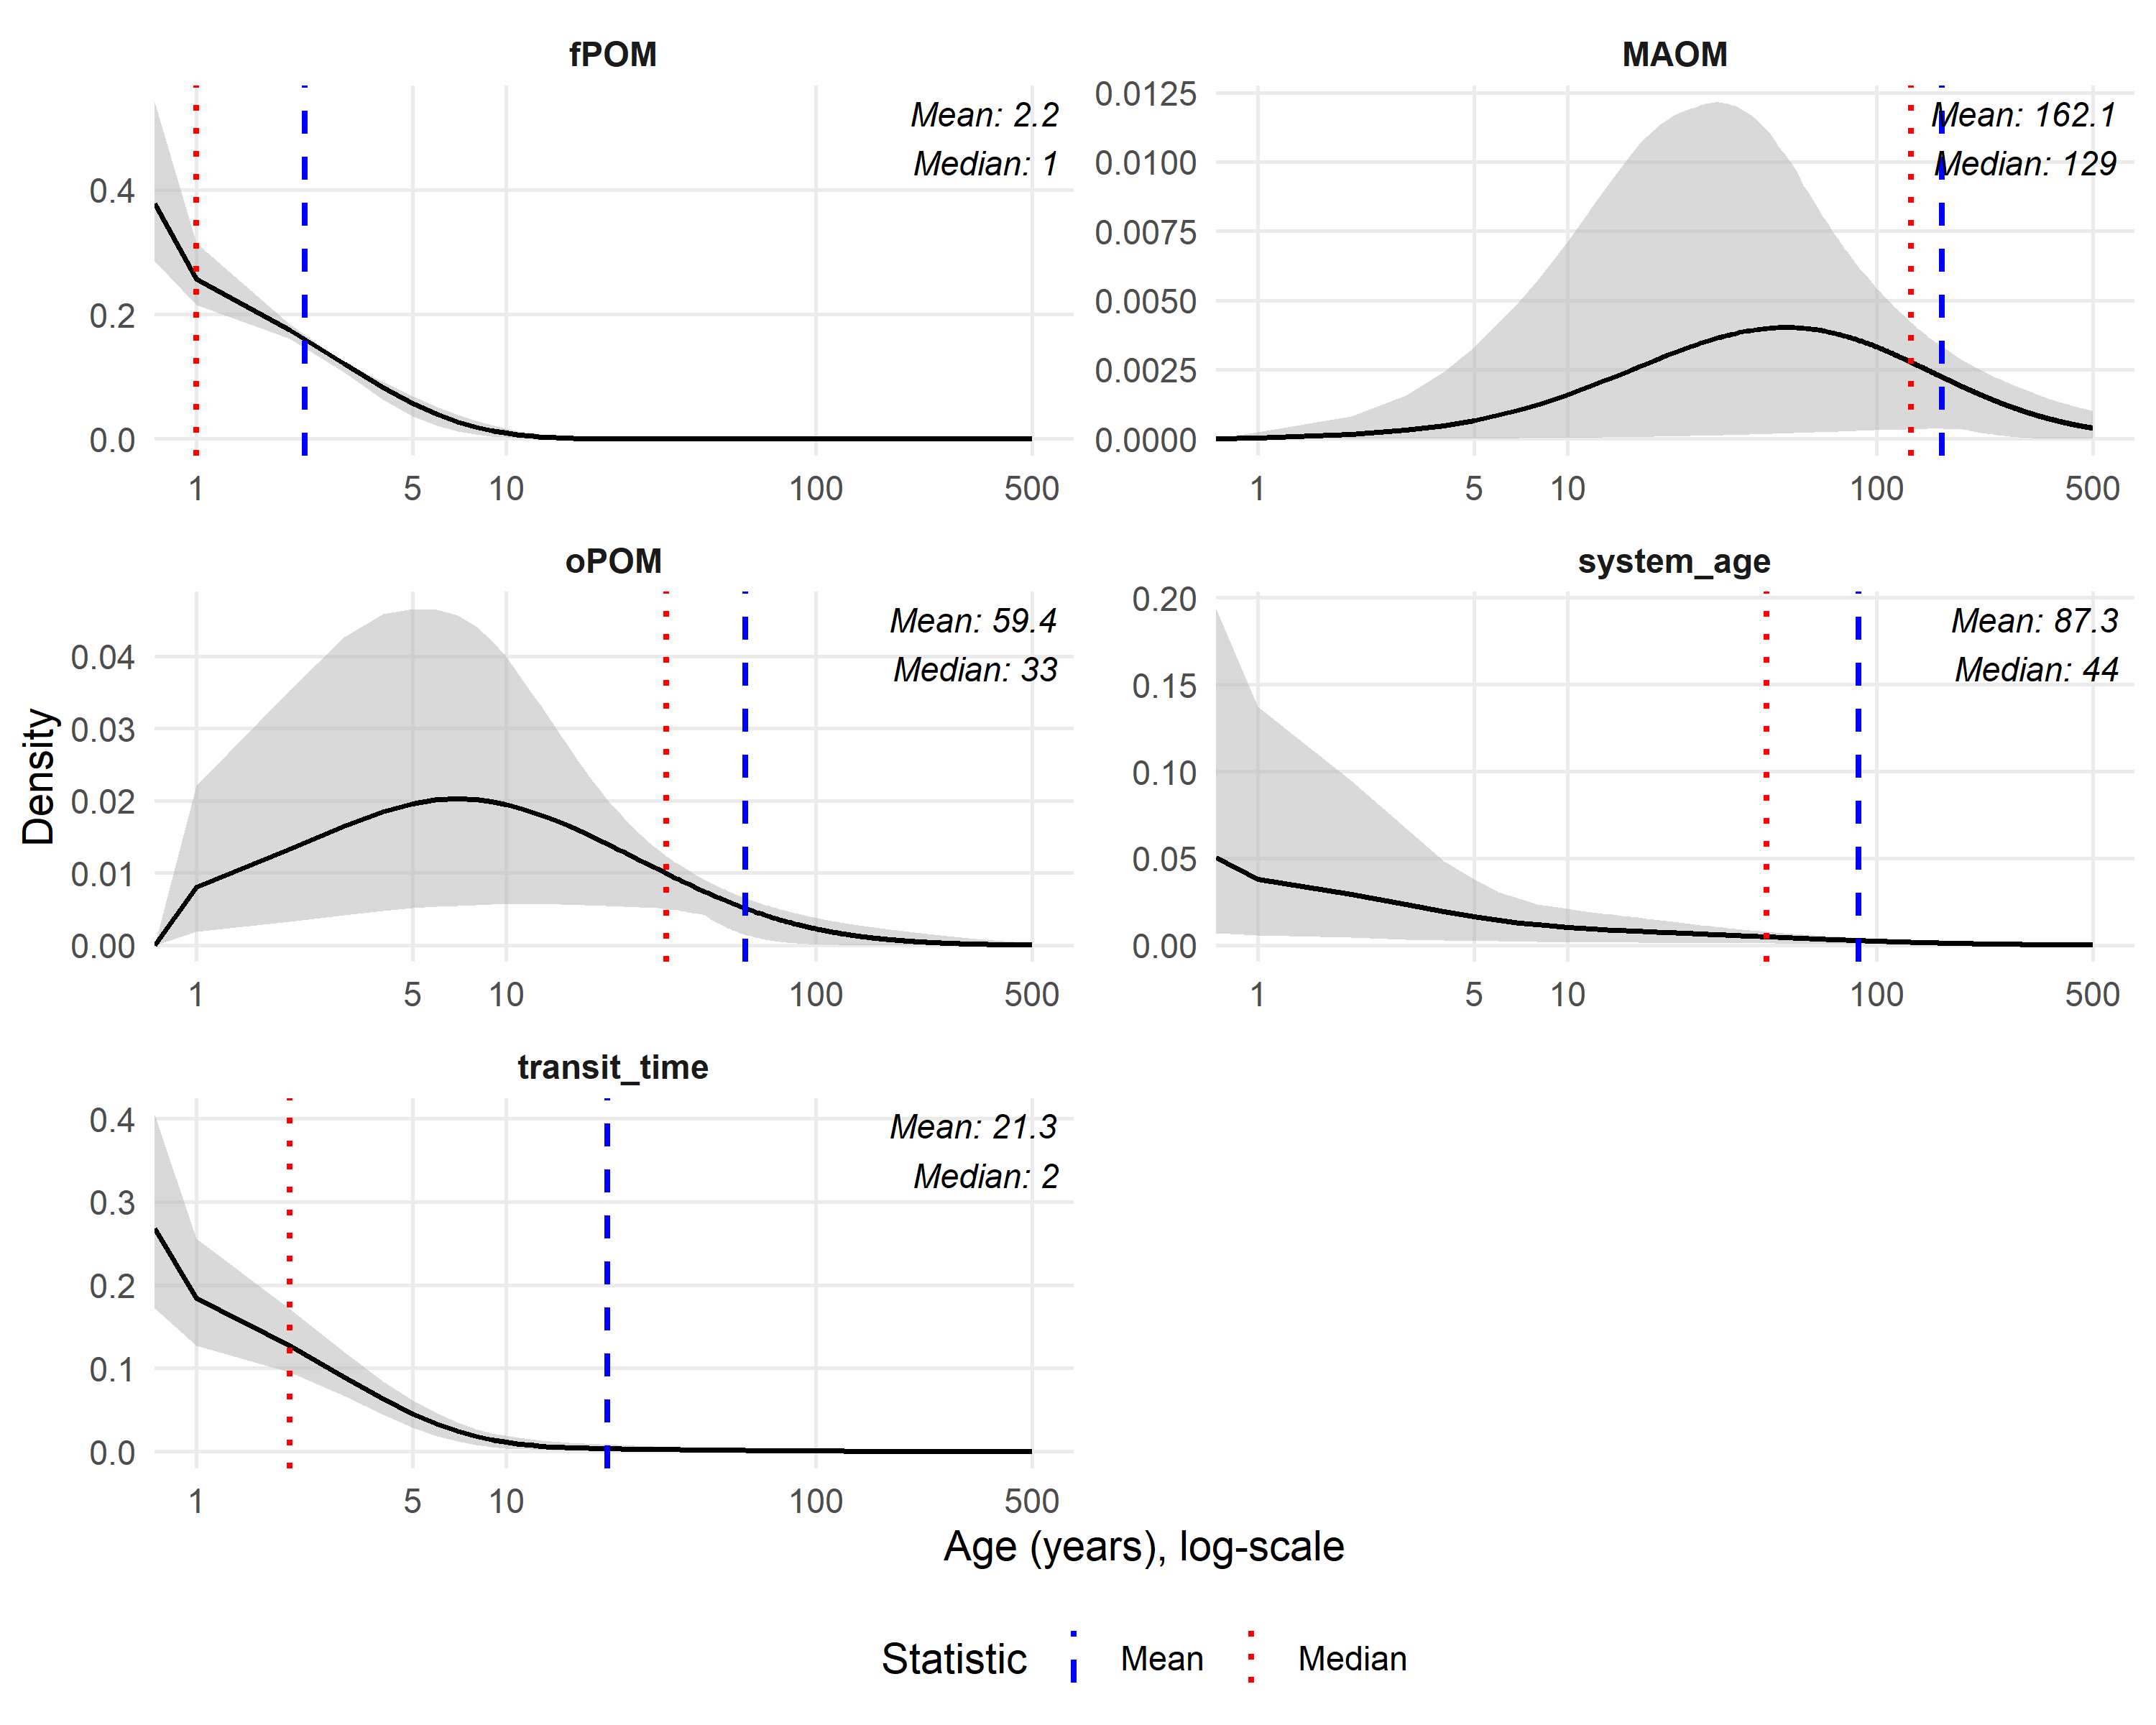
\includegraphics[width=1.0\textwidth]{figures/plot_log_age_tt_Lime.png} 
    \caption{Posterior distributions of SoilR-derived pool ages (fPOM, oPOM, MAOM) and whole-system carbon transit time (0--500 yr horizon) in soil amended with lime.}
    \label{fig:plot_log_age_tt_Lime}
\end{figure}

% residual plots for C and D14C prediction models from geochem pars

\newpage

\begin{figure}[htbp]
    \centering
    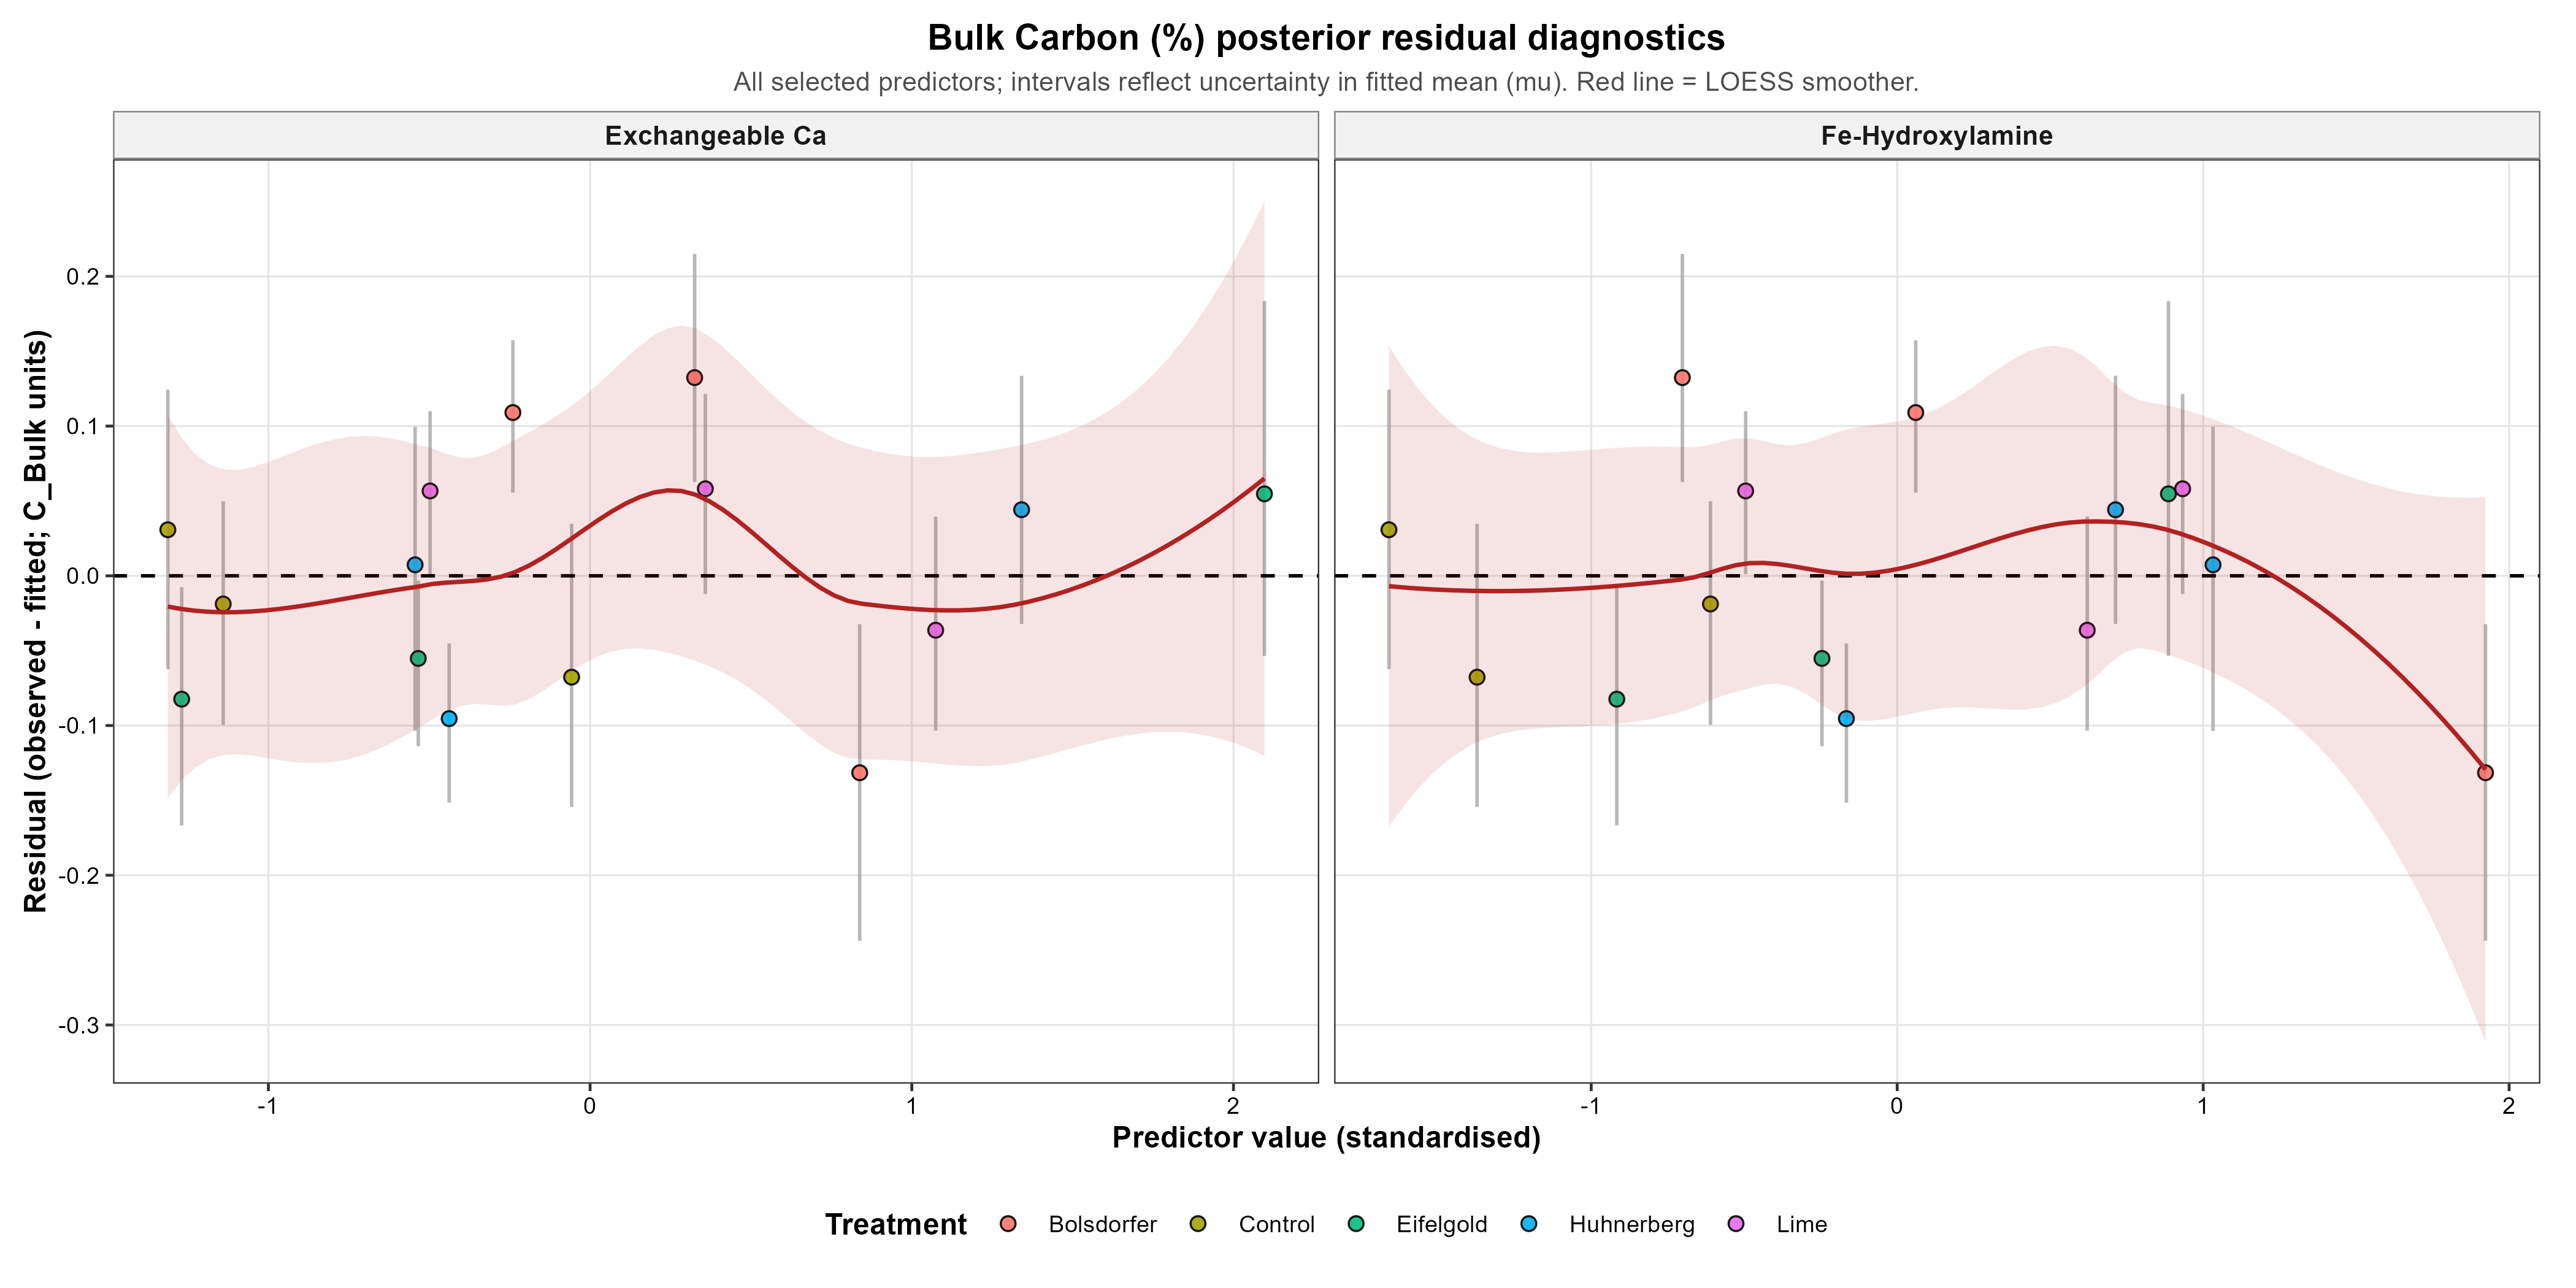
\includegraphics[width=1.0\textwidth]{figures/posterior_residuals_faceted_C_Bulk.png} 
    \caption{Posterior mean residuals and 95\% credible intervals plotted against selected predictors for the parsimonious projpred Bayesian models of bulk soil organic carbon concentration.}
    \label{fig:posterior_residuals_faceted_C_Bulk}
\end{figure}

\newpage

\begin{figure}[htbp]
    \centering
    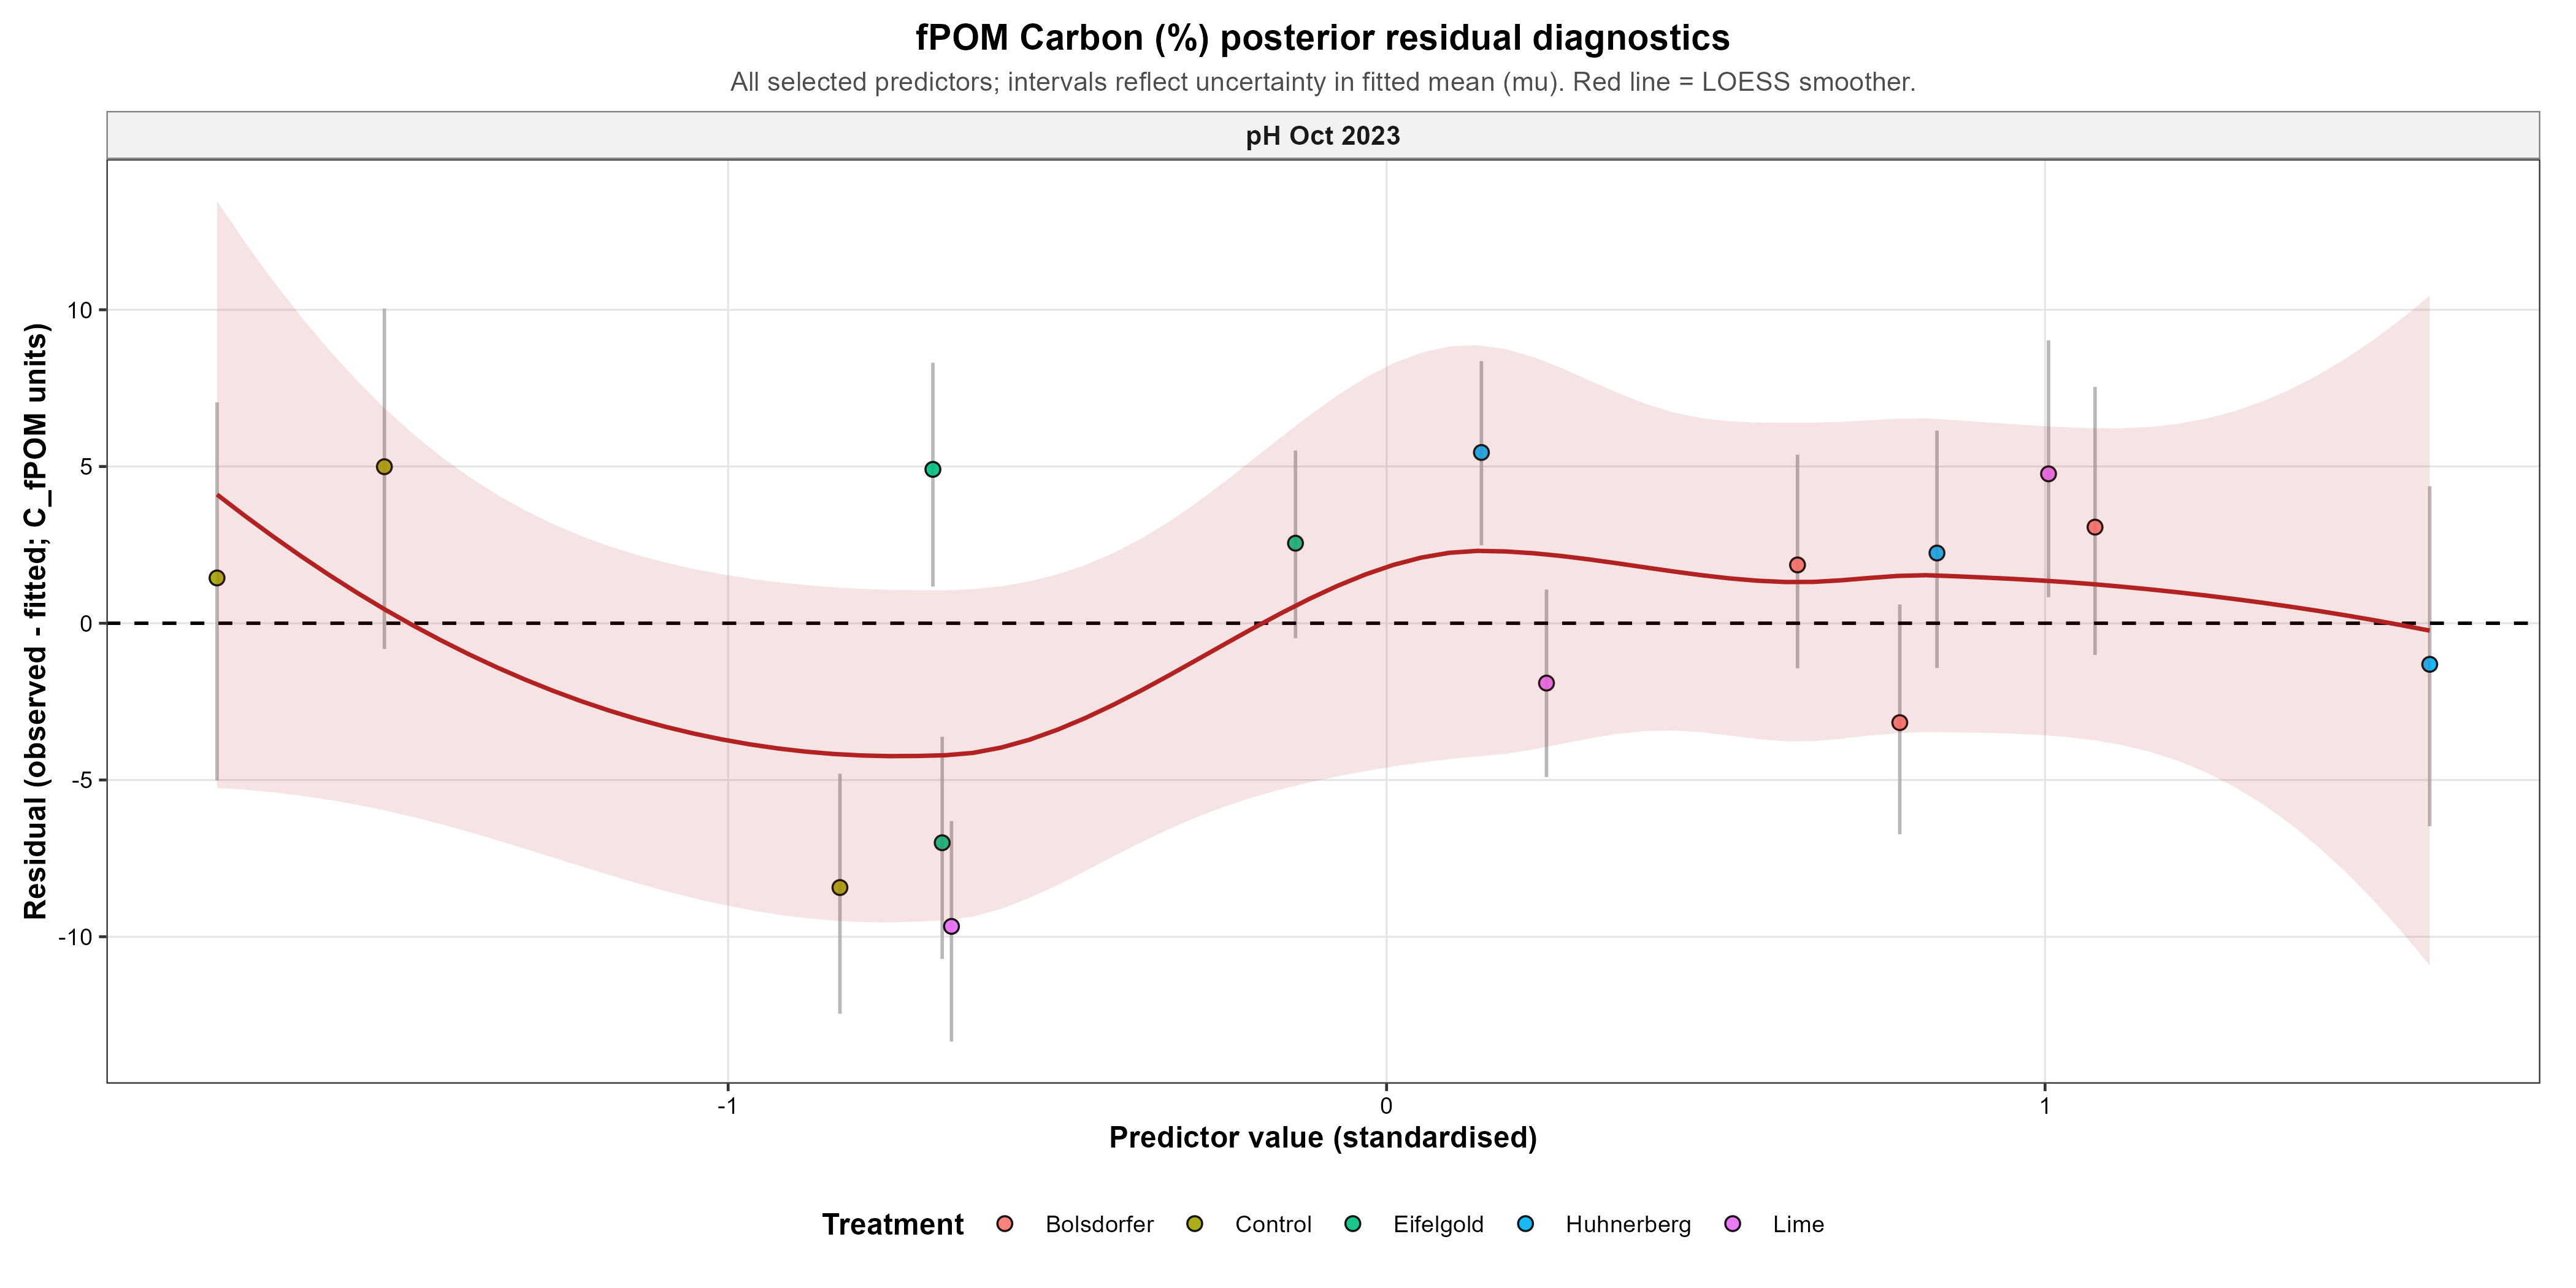
\includegraphics[width=1.0\textwidth]{figures/posterior_residuals_faceted_C_fPOM.png} 
    \caption{Posterior mean residuals and 95\% credible intervals plotted against selected predictors for the parsimonious projpred Bayesian models of fPOM organic carbon concentration.}
    \label{fig:posterior_residuals_faceted_C_fPOM}
\end{figure}


\newpage

\begin{figure}[htbp]
    \centering
    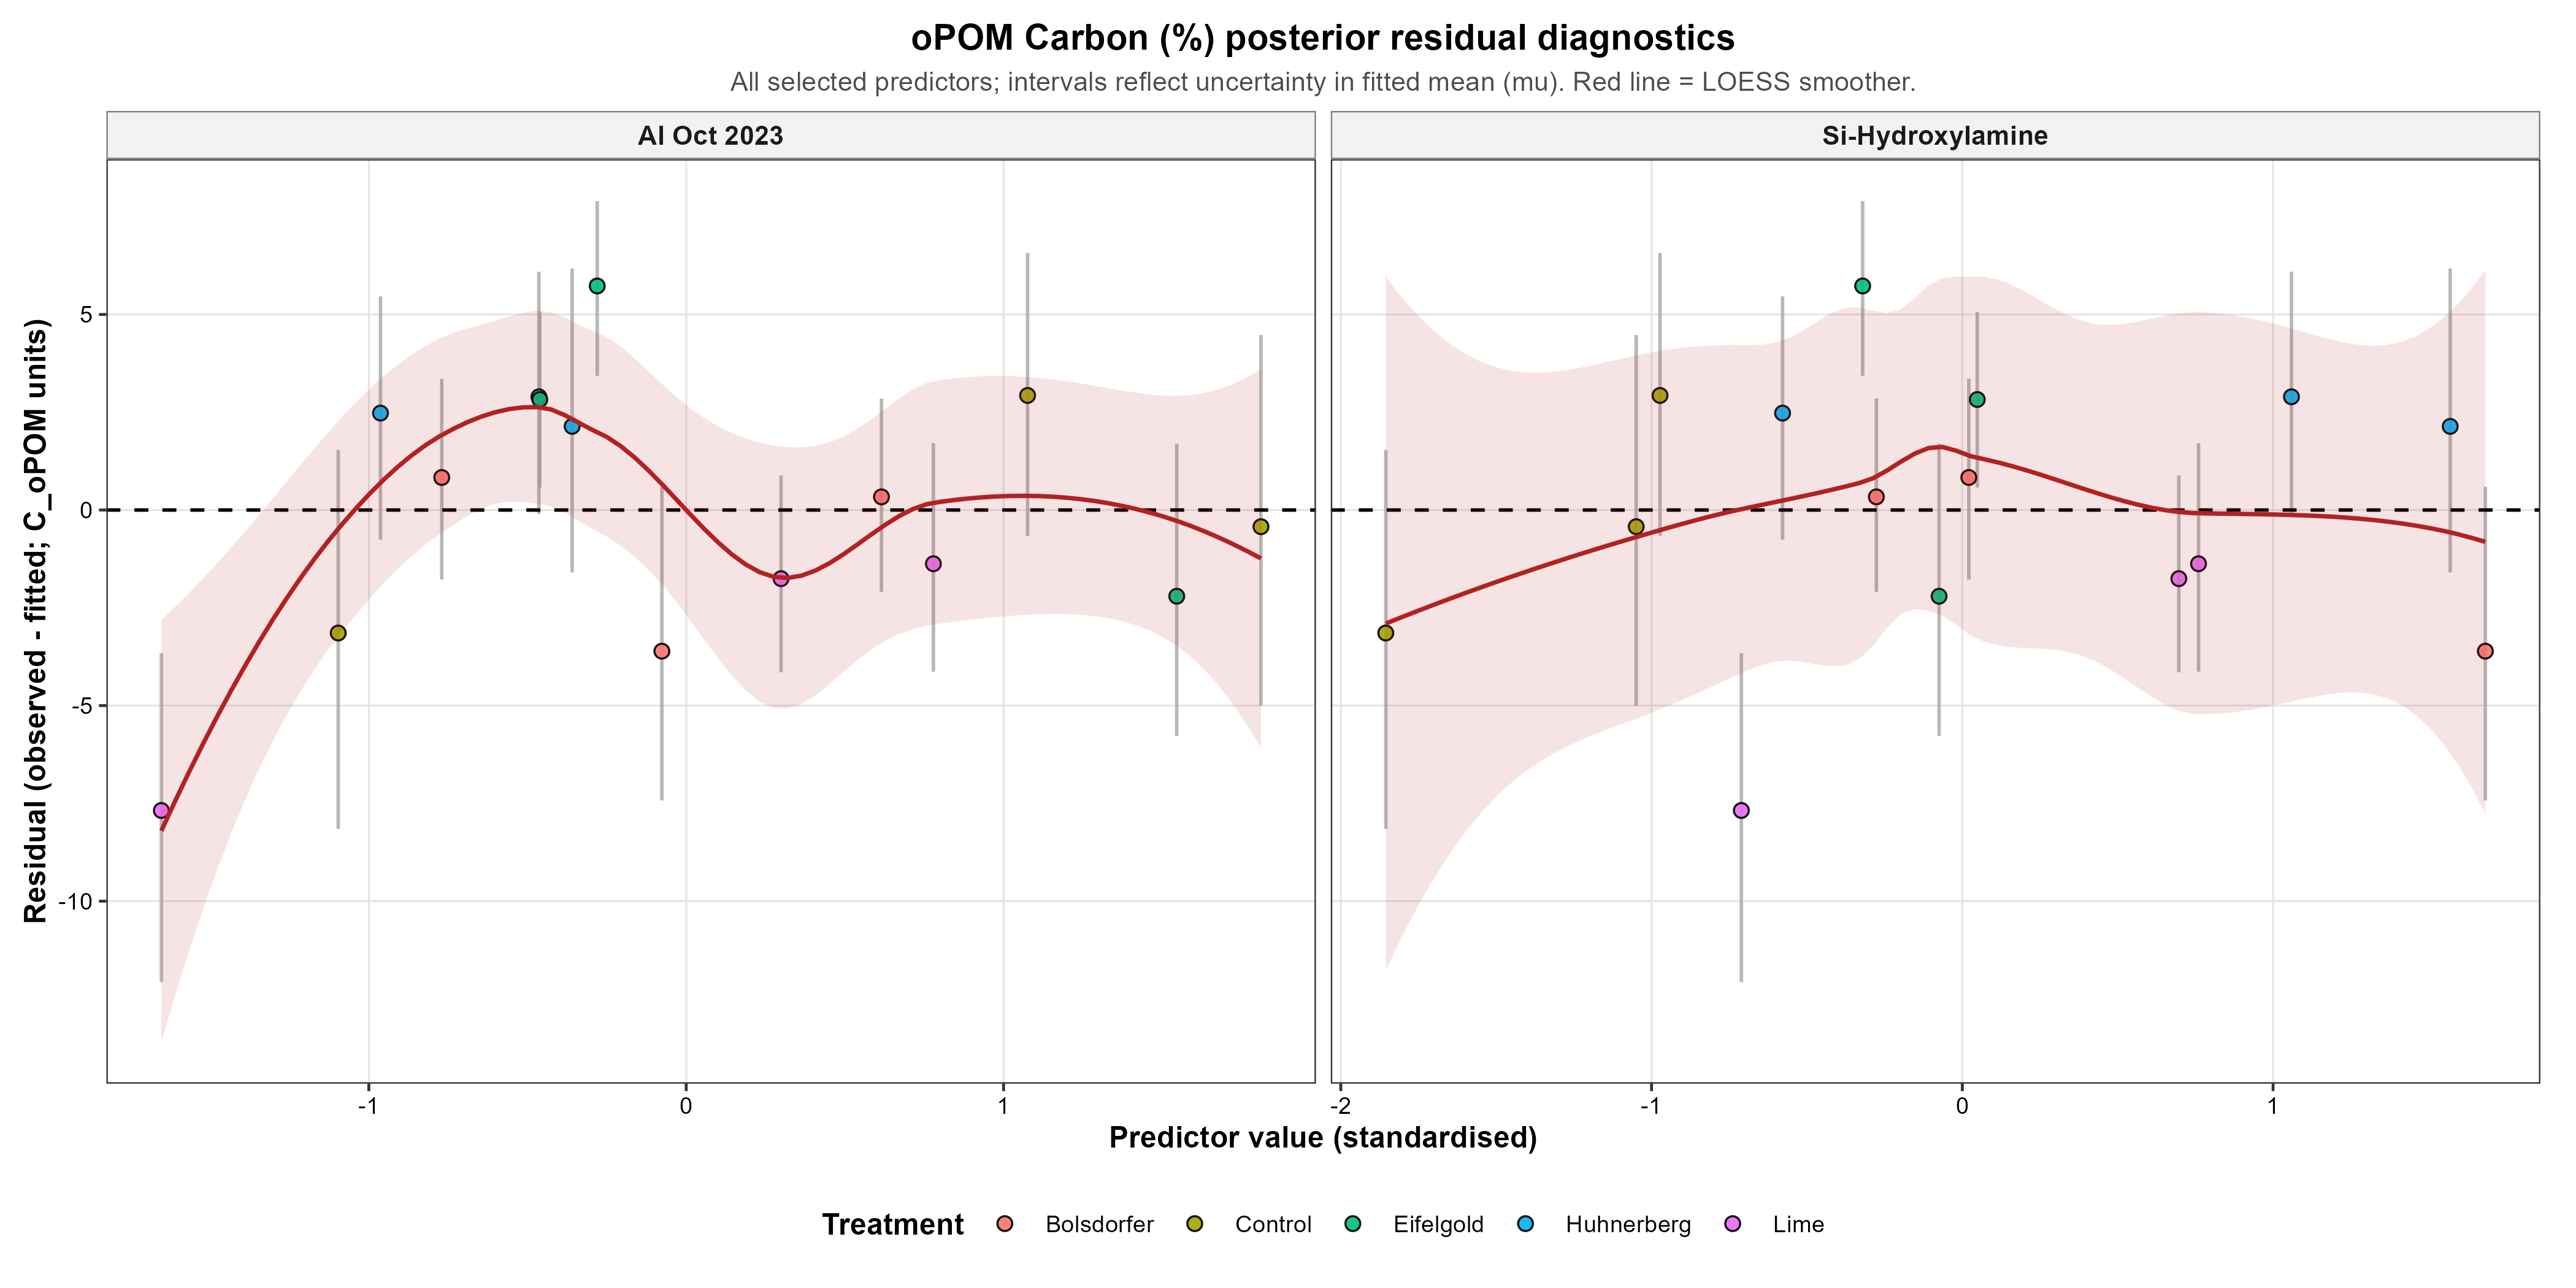
\includegraphics[width=1.0\textwidth]{figures/posterior_residuals_faceted_C_oPOM.png} 
    \caption{Posterior mean residuals and 95\% credible intervals plotted against selected predictors for the parsimonious projpred Bayesian models of oPOM organic carbon concentration.}
    \label{fig:posterior_residuals_faceted_C_oPOM}
\end{figure}

  
\newpage

\begin{figure}[htbp]
    \centering
    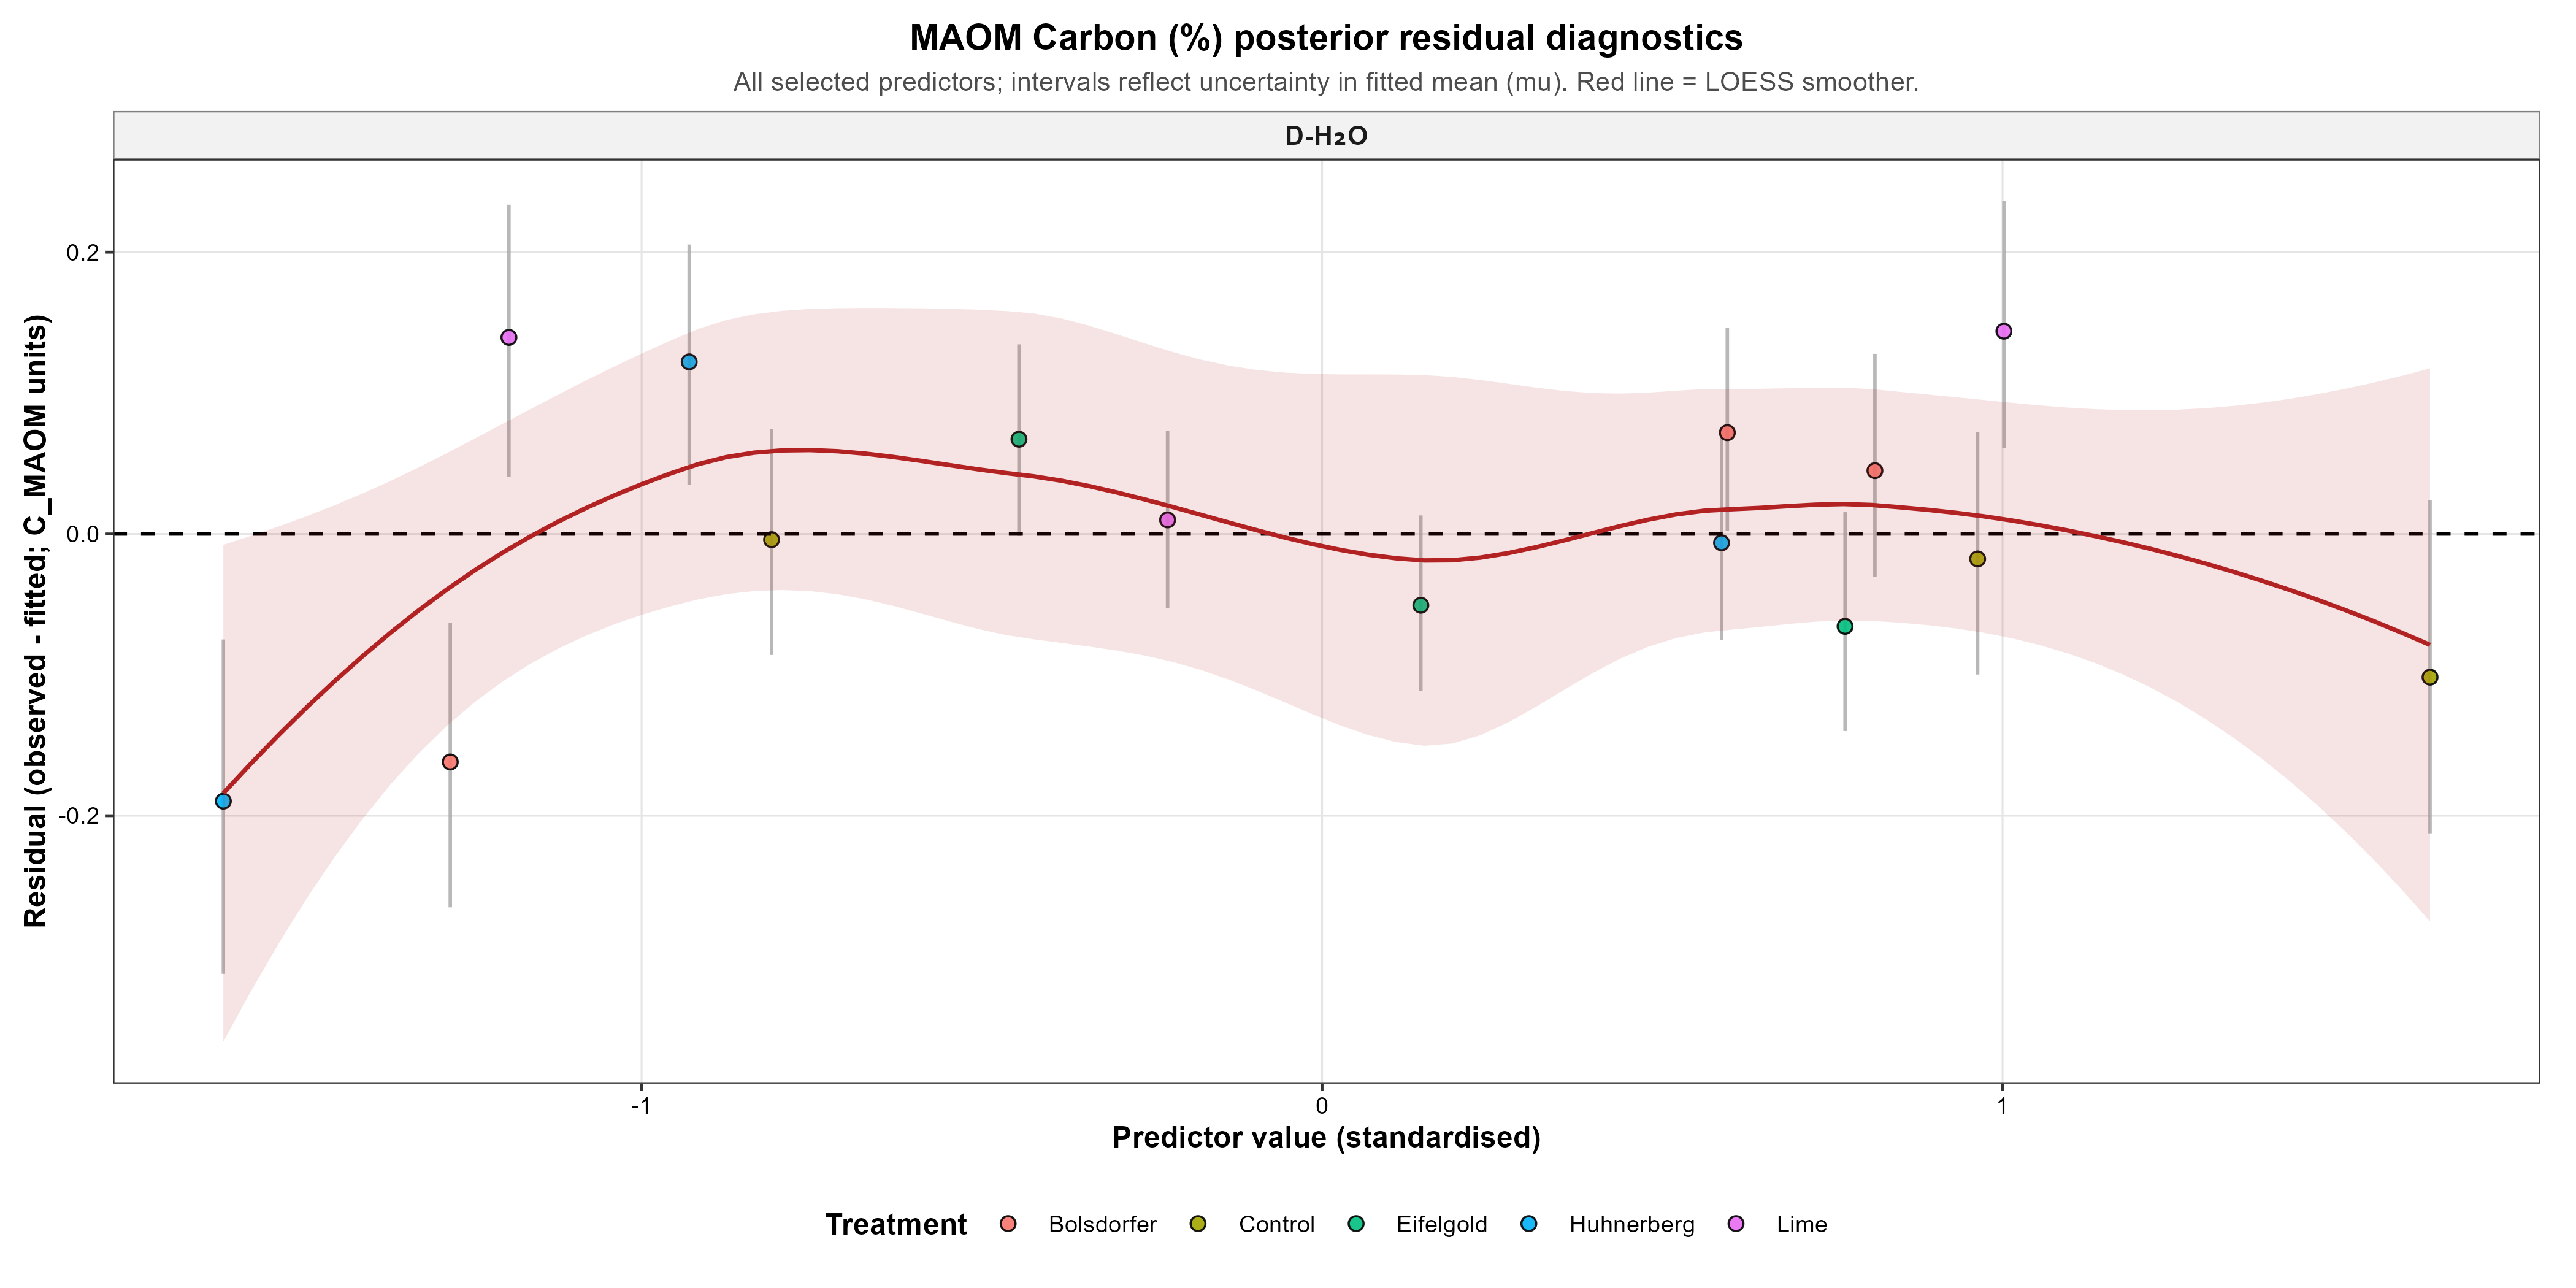
\includegraphics[width=1.0\textwidth]{figures/posterior_residuals_faceted_C_MAOM.png} 
    \caption{Posterior mean residuals and 95\% credible intervals plotted against selected predictors for the parsimonious projpred Bayesian models of MAOM organic carbon concentration.}
    \label{fig:posterior_residuals_faceted_C_MAOM}
\end{figure}


\newpage

\begin{figure}[htbp]
    \centering
    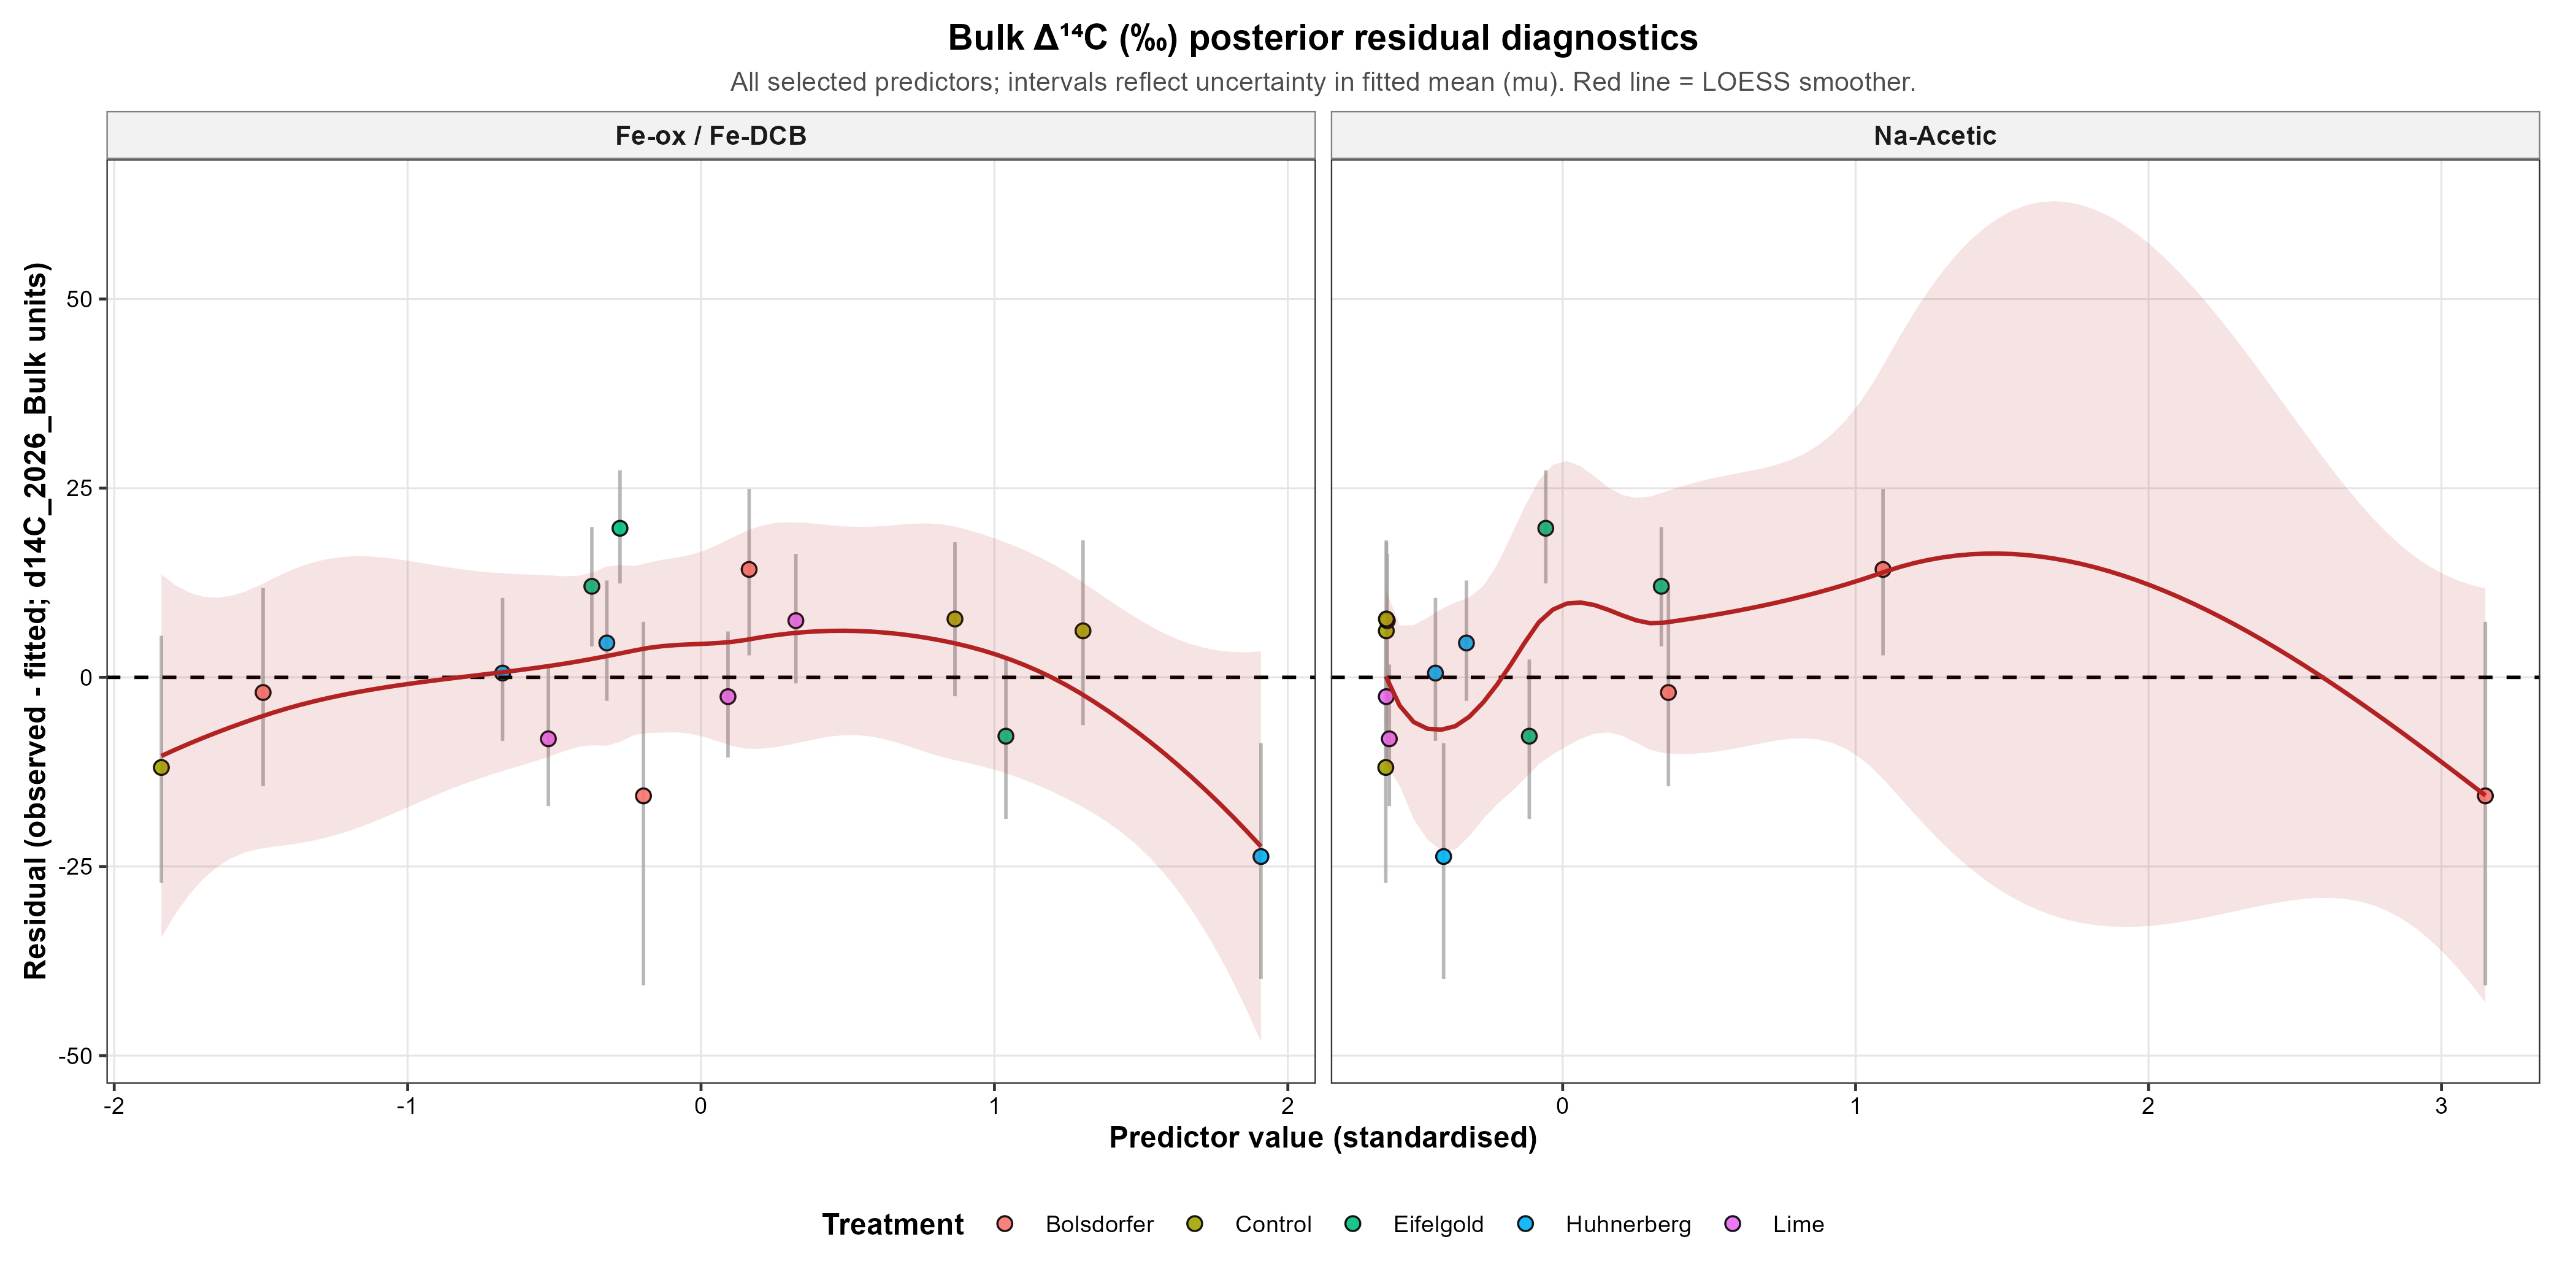
\includegraphics[width=1.0\textwidth]{figures/posterior_residuals_faceted_d14C_2026_Bulk.png} 
    \caption{Posterior mean residuals and 95\% credible intervals plotted against selected predictors for the parsimonious projpred Bayesian models of bulk soil $\Delta^{14}\text{C}$ (2026). }
    \label{fig:posterior_residuals_faceted_d14C_2026_Bulk}
\end{figure}

  
\newpage

\begin{figure}[htbp]
    \centering
    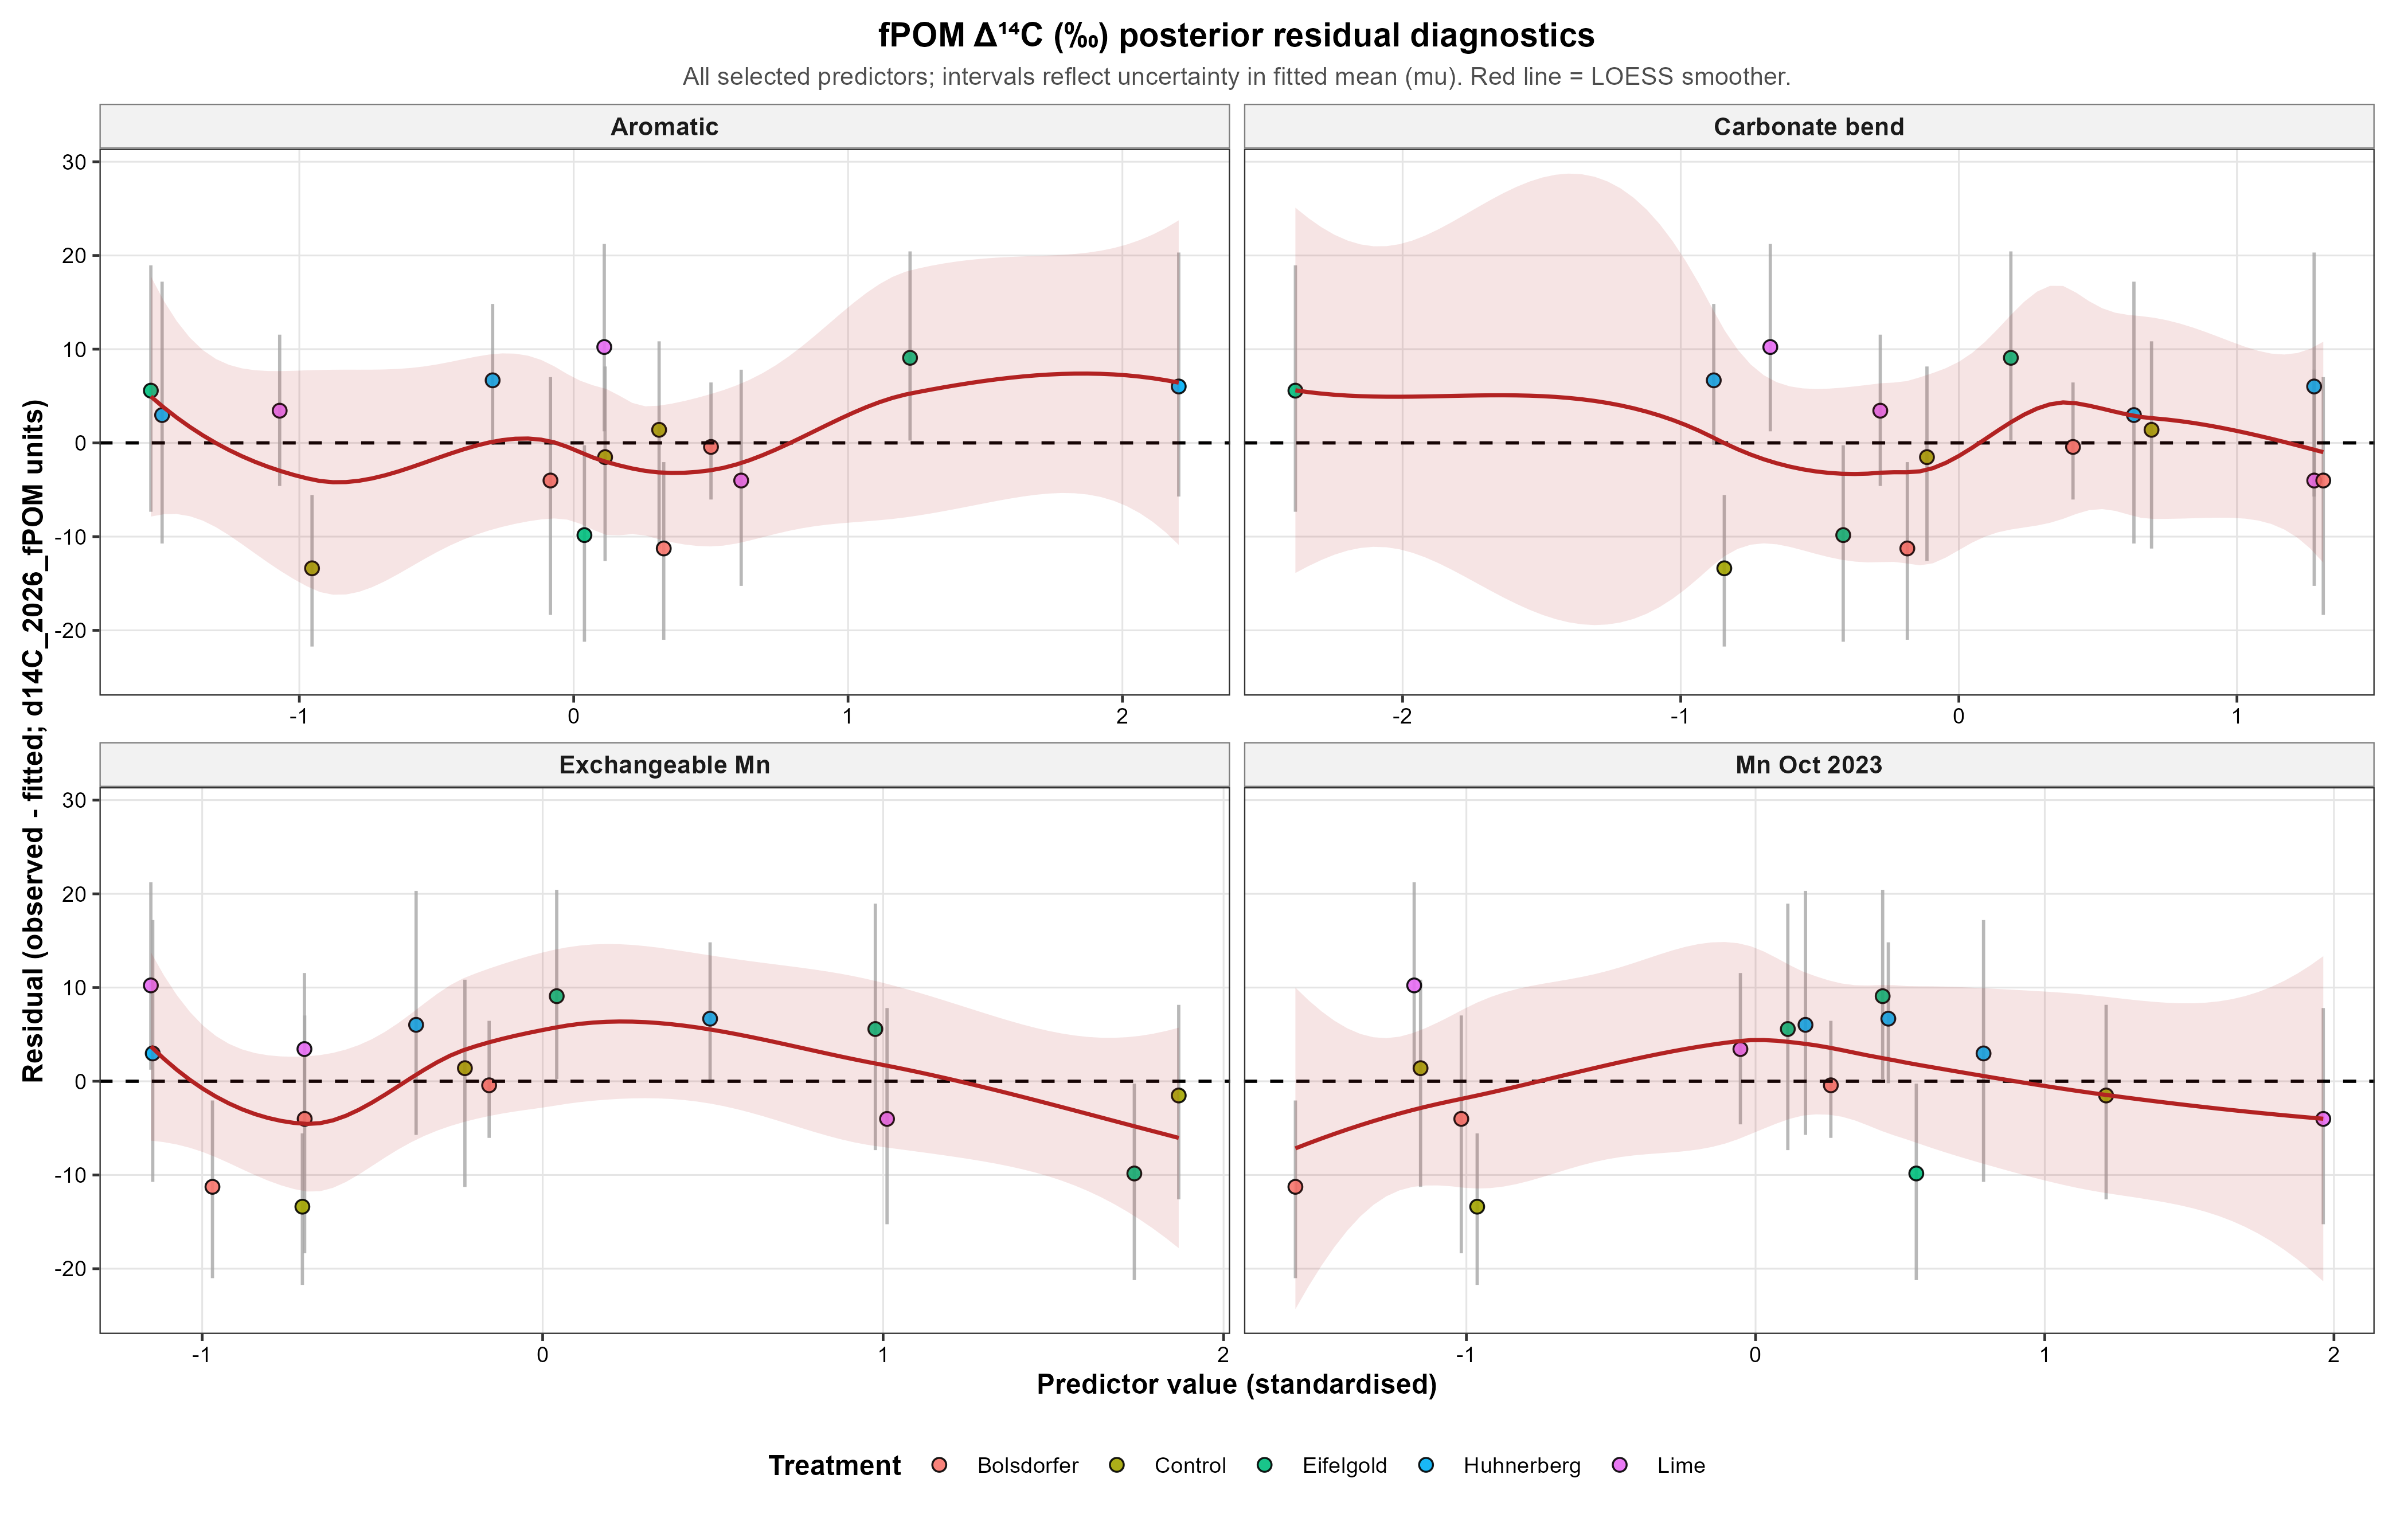
\includegraphics[width=1.0\textwidth]{figures/posterior_residuals_faceted_d14C_2026_fPOM.png} 
    \caption{Posterior mean residuals and 95\% credible intervals plotted against selected predictors for the parsimonious projpred Bayesian models of fPOM $\Delta^{14}\text{C}$ (2026). }
    \label{fig:posterior_residuals_faceted_d14C_2026_fPOM}
\end{figure}
  
\newpage

\begin{figure}[htbp]
    \centering
    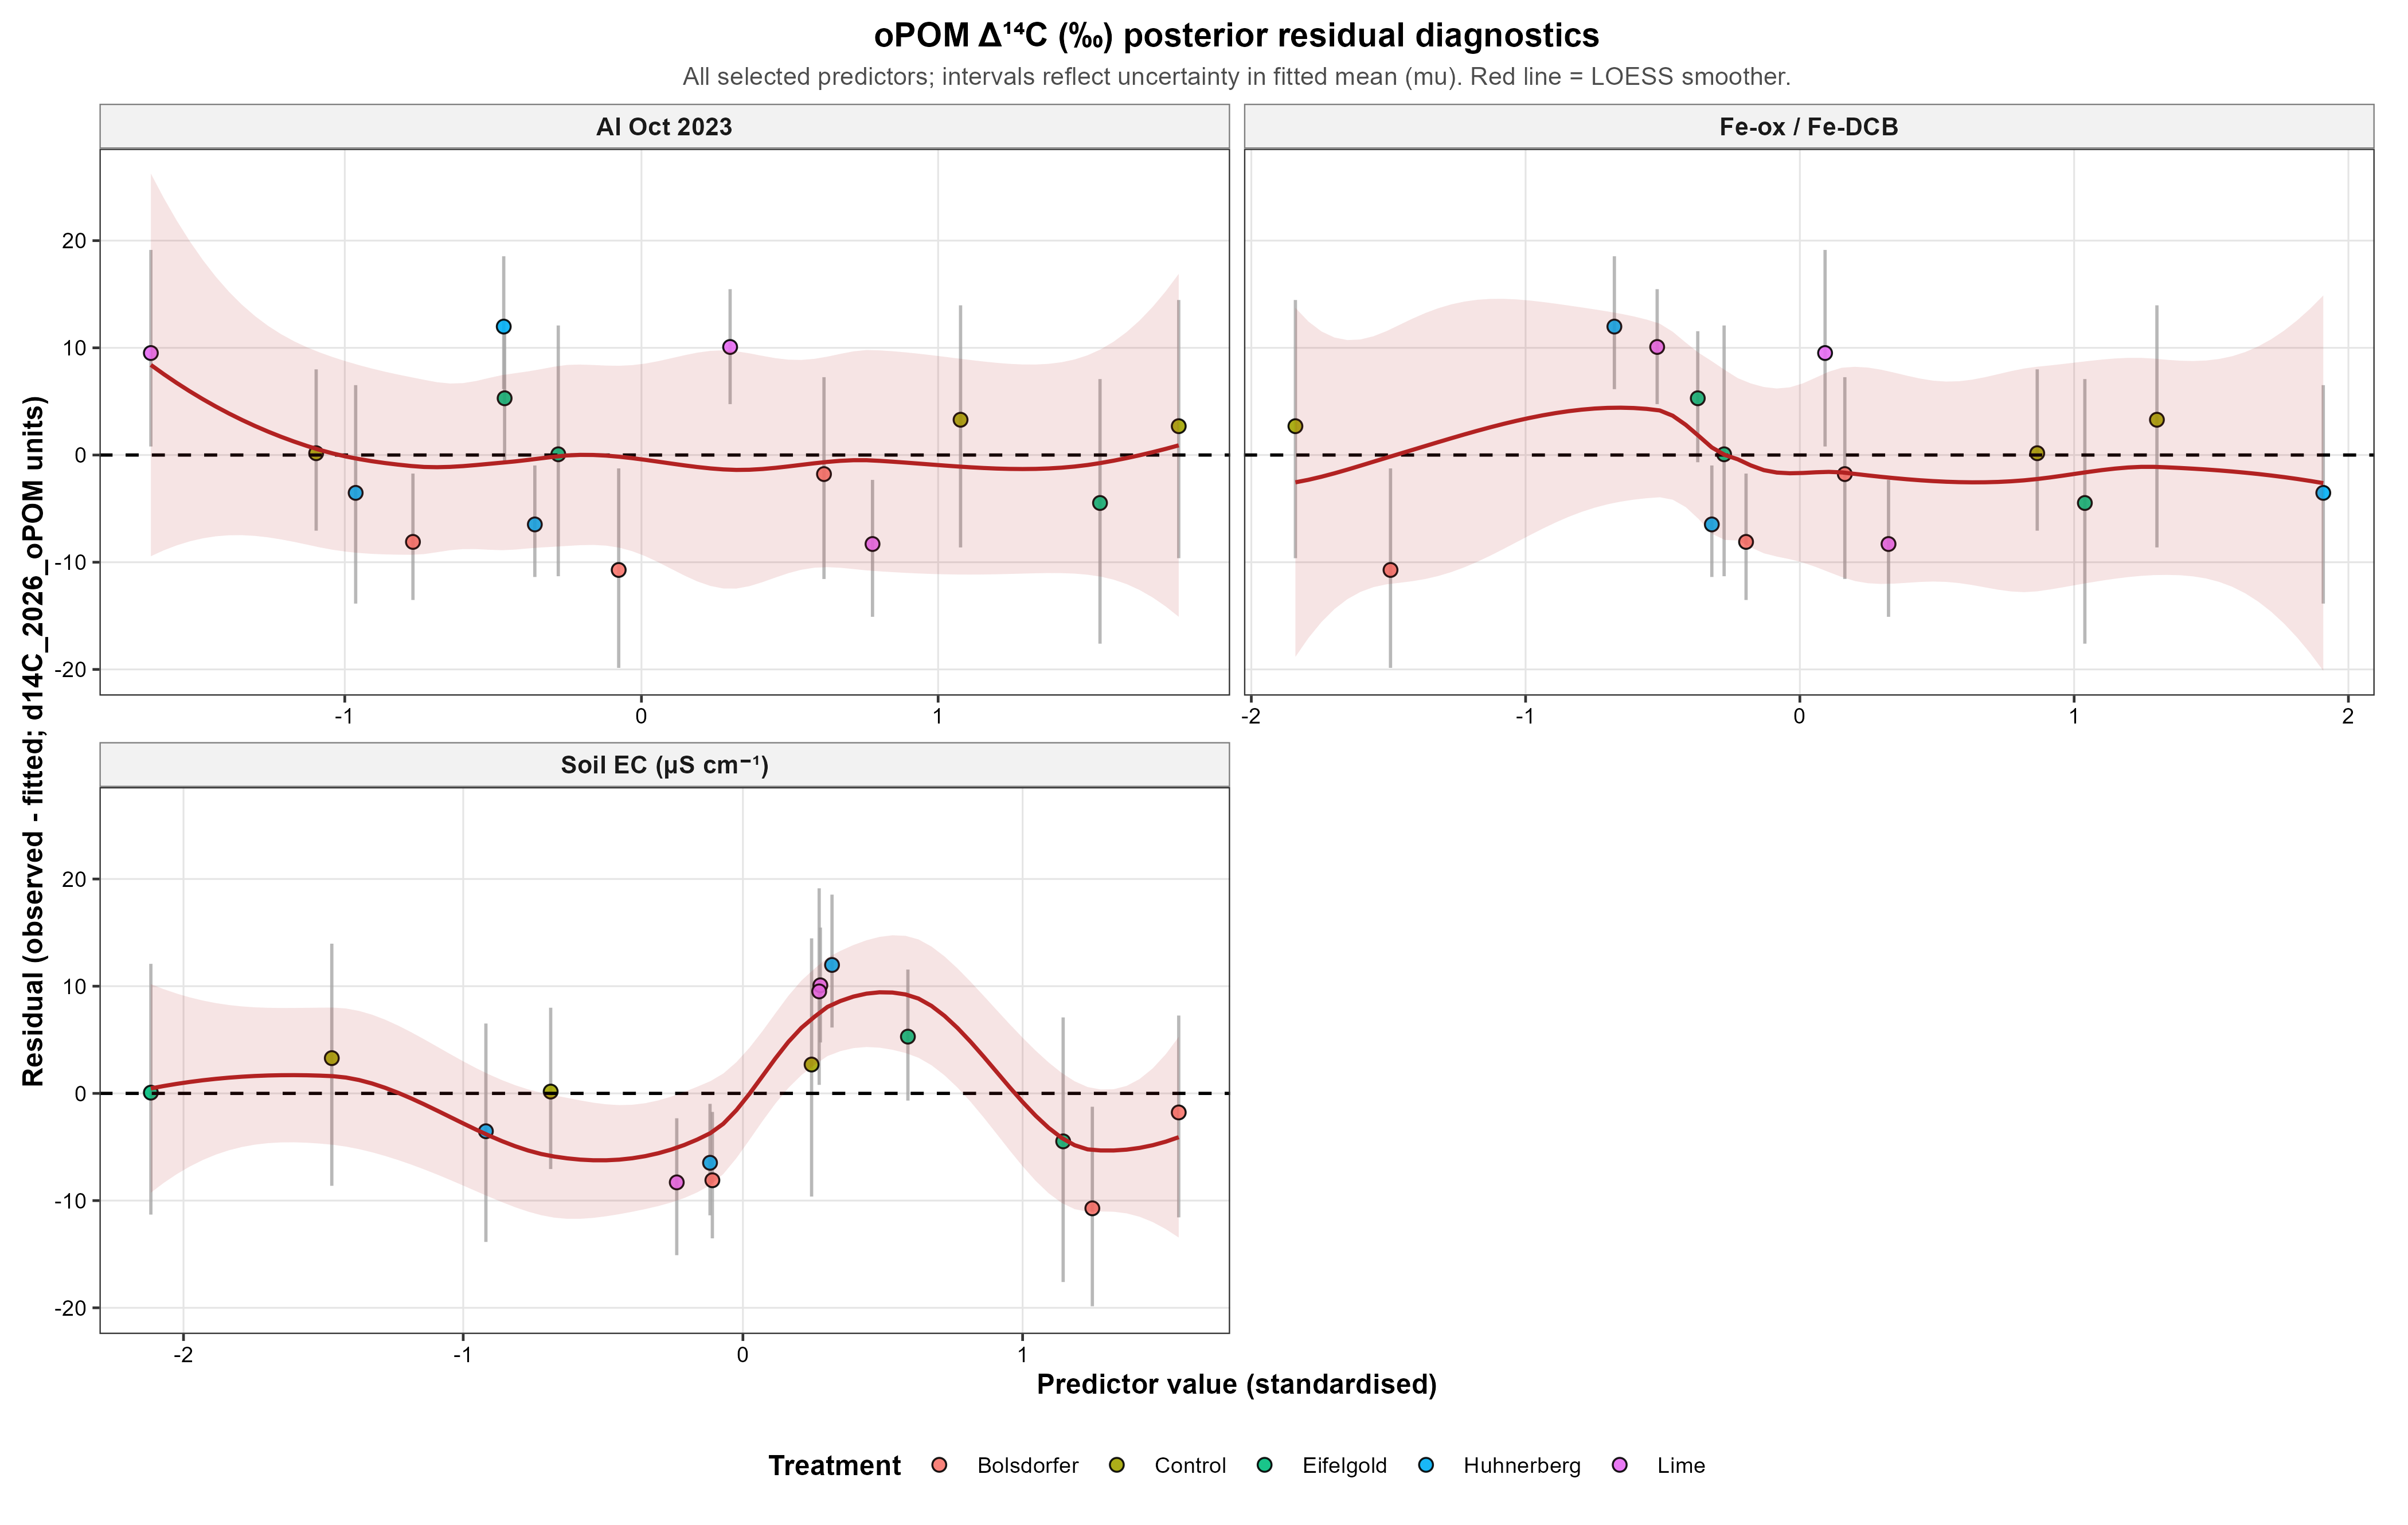
\includegraphics[width=1.0\textwidth]{figures/posterior_residuals_faceted_d14C_2026_oPOM.png} 
    \caption{Posterior mean residuals and 95\% credible intervals plotted against selected predictors for the parsimonious projpred Bayesian models of oPOM $\Delta^{14}\text{C}$ (2026). }
    \label{fig:posterior_residuals_faceted_d14C_2026_oPOM}
\end{figure}

  
\newpage

\begin{figure}[htbp]
    \centering
    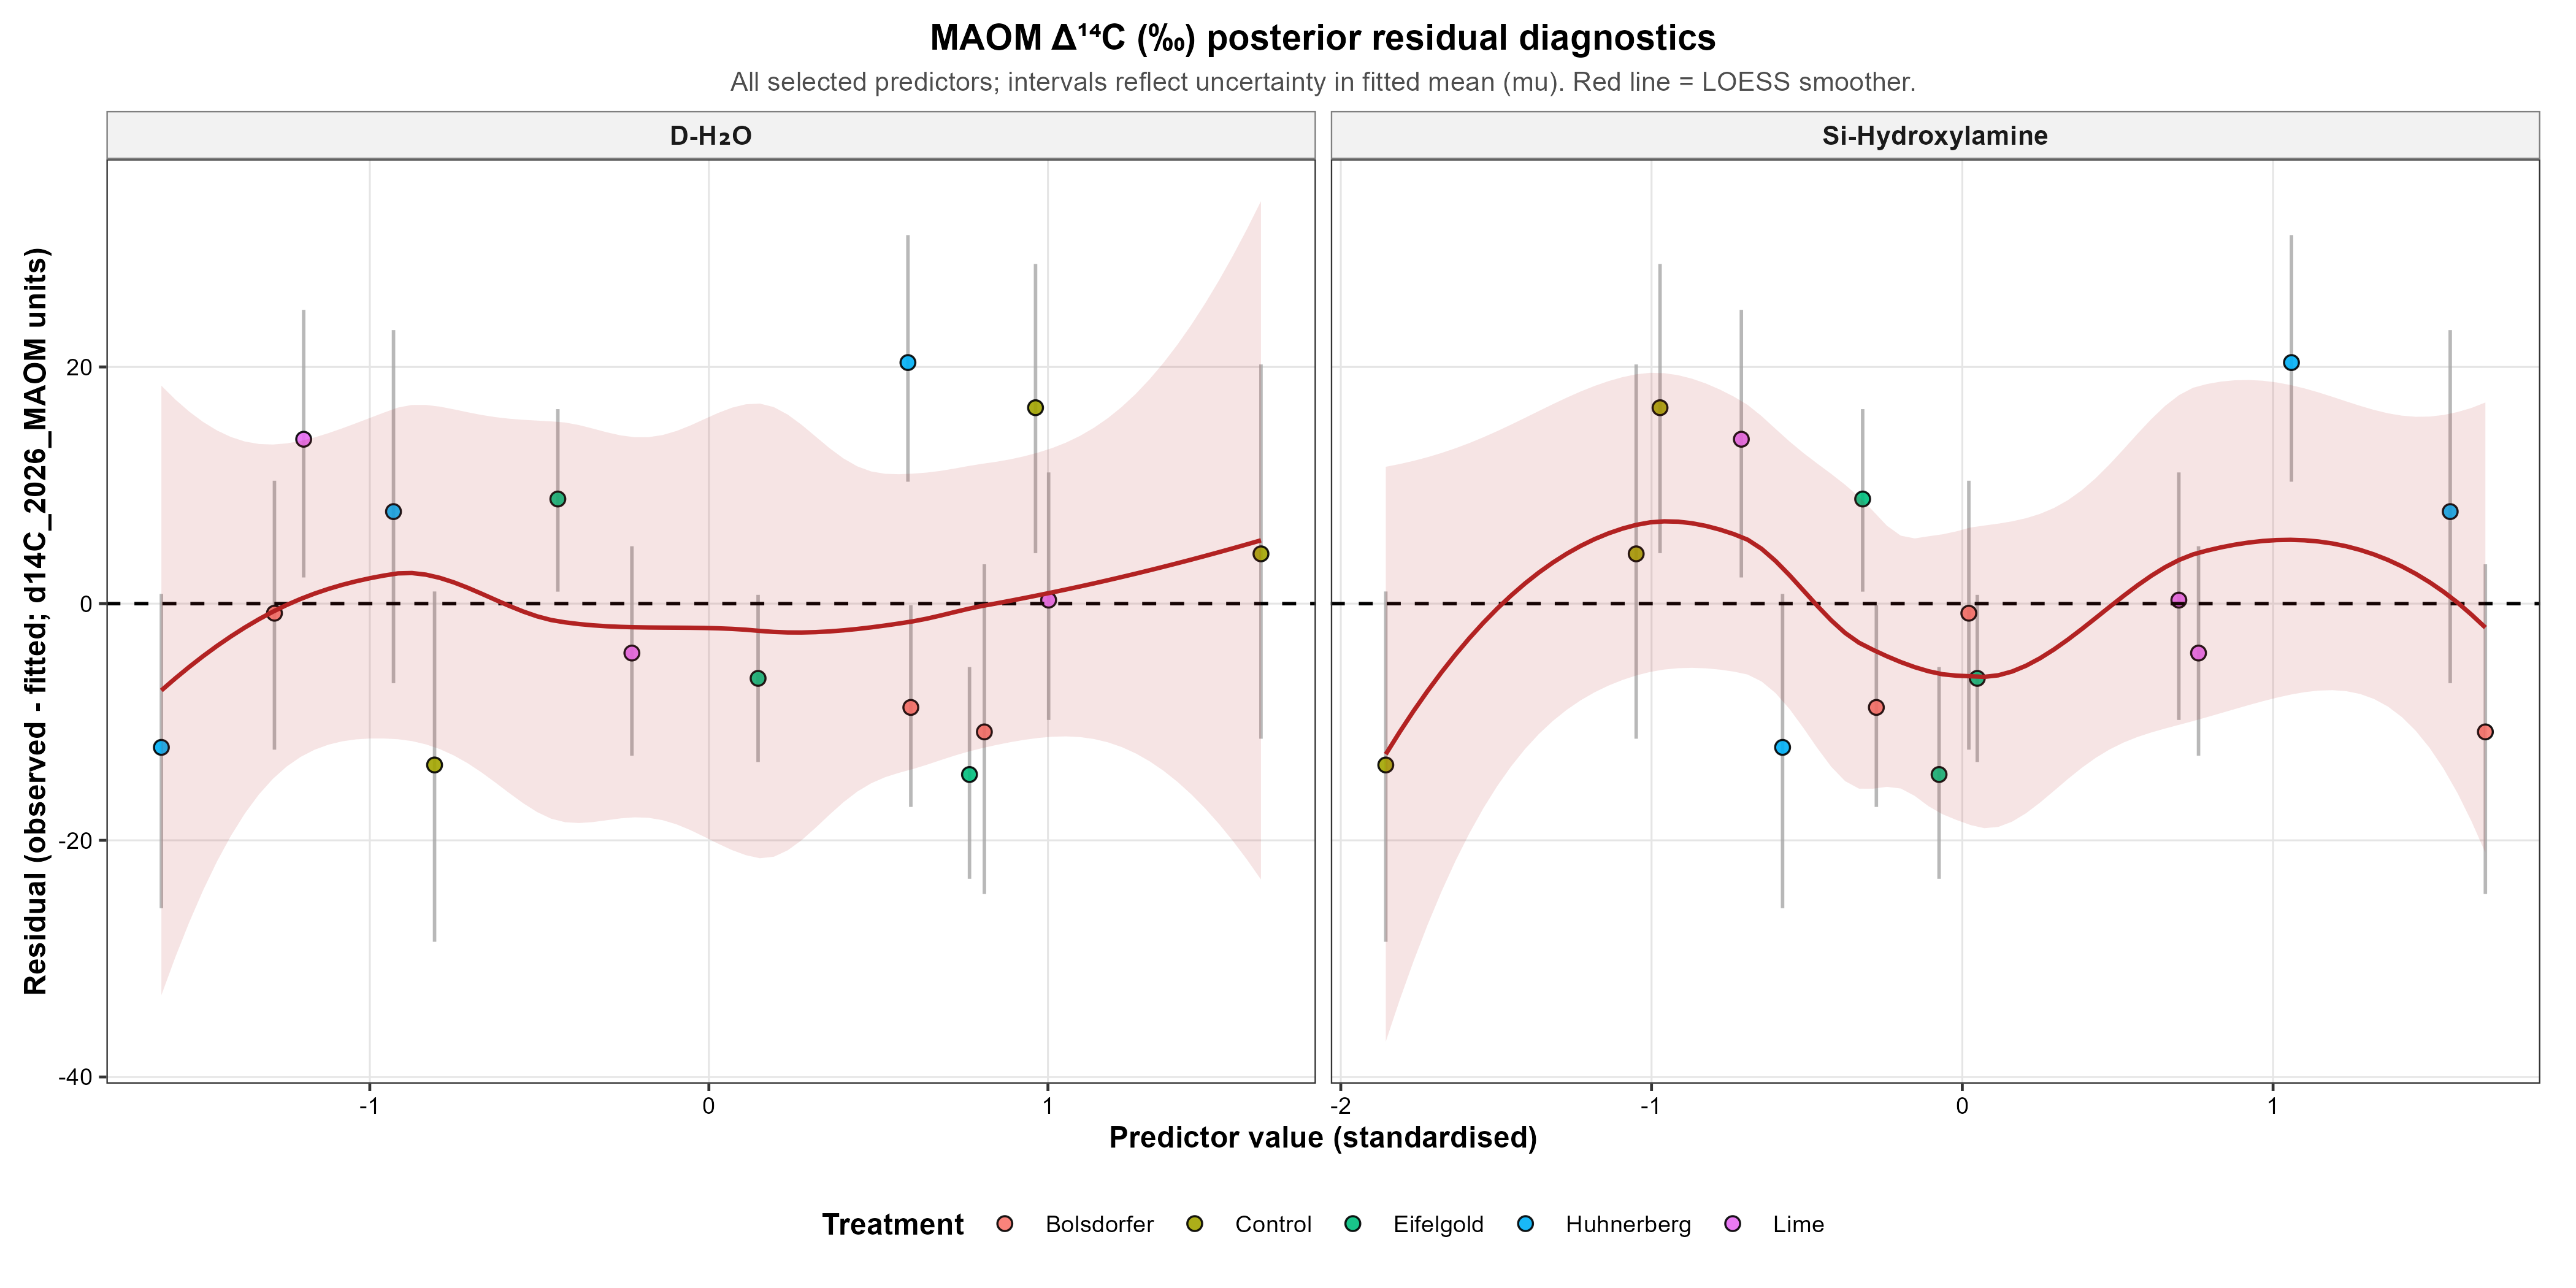
\includegraphics[width=1.0\textwidth]{figures/posterior_residuals_faceted_d14C_2026_MAOM.png} 
    \caption{Posterior mean residuals and 95\% credible intervals plotted against selected predictors for the parsimonious projpred Bayesian models of MAOM $\Delta^{14}\text{C}$ (2026).}
    \label{fig:posterior_residuals_faceted_d14C_2026_MAOM}
\end{figure}


\end{document}